\documentclass[10pt]{report}
\usepackage[centertags]{amsmath}
\usepackage{amsfonts}
\usepackage{amssymb}
\usepackage{amsthm}
\usepackage{newlfont}
\usepackage{graphicx}
%\usepackage[super,sort&compress]{natbib}
%\usepackage[sort&compress]{natbib}
%\usepackage[numbers]{natbib}
\usepackage[authoryear,square]{natbib}


\hfuzz2pt
\newlength{\defbaselineskip}
\setlength{\defbaselineskip}{\baselineskip}
\newcommand{\setlinespacing}[1]%
           {\setlength{\baselineskip}{#1 \defbaselineskip}}
\newcommand{\doublespacing}{\setlength{\baselineskip}%
                           {2.0 \defbaselineskip}}
\newcommand{\singlespacing}{\setlength{\baselineskip}{\defbaselineskip}}
\newcommand{\A}{{\cal A}}
\newcommand{\h}{{\cal H}}
\newcommand{\s}{{\cal S}}
\newcommand{\W}{{\cal W}}
\newcommand{\BH}{\mathbf B(\cal H)}
\newcommand{\KH}{\cal  K(\cal H)}
\newcommand{\Real}{\mathbb R}
\newcommand{\Complex}{\mathbb C}
\newcommand{\Field}{\mathbb F}
\newcommand{\RPlus}{[0,\infty)}
\newcommand{\norm}[1]{\left\Vert#1\right\Vert}
\newcommand{\essnorm}[1]{\norm{#1}_{\text{\rm\normalshape ess}}}
\newcommand{\abs}[1]{\left\vert#1\right\vert}
\newcommand{\set}[1]{\left\{#1\right\}}
\newcommand{\seq}[1]{\left<#1\right>}
\newcommand{\eps}{\varepsilon}
\newcommand{\To}{\longrightarrow}
\newcommand{\RE}{\operatorname{Re}}
\newcommand{\IM}{\operatorname{Im}}
\newcommand{\Poly}{{\cal{P}}(E)}
\newcommand{\EssD}{{\cal{D}}}
\theoremstyle{plain}
\newtheorem{thm}{Theorem}[section]
\newtheorem{cor}[thm]{Corollary}
\newtheorem{lem}[thm]{Lemma}
\newtheorem{prop}[thm]{Proposition}
\theoremstyle{definition}
\newtheorem{defn}{Definition}[section]
\theoremstyle{remark}
\newtheorem{rem}{Remark}[section]

\newcommand{\field}[1]{\mathbb{#1}}
\newcommand{\C}{\field{C}}
\newcommand{\R}{\field{R}}
\newcommand{\script}[1]{\mathcal{#1}}
\DeclareSymbolFont{AMSb}{U}{msb}{m}{n}
\DeclareMathSymbol{\dbln}{\mathalpha}{AMSb}{"4E}
\DeclareMathSymbol{\dblp}{\mathalpha}{AMSb}{"50}
\DeclareMathSymbol{\dblz}{\mathalpha}{AMSb}{"5A}
\DeclareMathSymbol{\dblr}{\mathalpha}{AMSb}{"52}
\DeclareMathSymbol{\dblt}{\mathalpha}{AMSb}{"54}
\DeclareMathSymbol{\dblq}{\mathalpha}{AMSb}{"51}
\DeclareMathSymbol{\dbln}{\mathalpha}{AMSb}{"4E}
\DeclareMathSymbol{\dblf}{\mathalpha}{AMSb}{"46}
\DeclareMathSymbol{\dblc}{\mathalpha}{AMSb}{"43}
\DeclareMathSymbol{\dbld}{\mathalpha}{AMSb}{"44}
\newcommand{\fall}{\; \forall \;}
\newcommand{\exts}{\; \exists \;}
\newcommand{\st}{\; \ni \;}
\newcommand{\mbf}[1]{\mathbf{#1}}
\newcommand{\binomial}[2]{\biggl( \begin{array}{c}  #1 \\ #2  \\ \end{array} \biggr) }
\newcommand{\fderiv}[2]{ \frac{d}{ d #1} \: #2}
\newcommand{\sderiv}[2]{ \frac{d^2}{ d^2 #1} \: #2}
\newcommand{\pfderiv}[2]{ \frac{\partial}{ \partial #1} \: #2}
\newcommand{\psderiv}[2]{ \frac{\partial^2}{ \partial^2 #1} \: #2}
\newcommand{\mat}[1]{\mathbf{#1}}

\numberwithin{equation}{section}
\renewcommand{\theequation}{\thesection.\arabic{equation}}

\title{A Field Guide for Machine Learning, Computer Vision and Numerical Linear Algebra}

\author{Bruce B. Campbell}

\begin{document}

{ \typeout{A Field Guide for Machine Learning, Computer Vision and Numerical Linear Algebra}
\include{ABS}
}

{ \typeout{Acknowledgements}
\include{ACK}
}
\def\baselinestretch{1}
\setlinespacing{1.0}

\setcounter{page}{1}
\tableofcontents

{ \typeout{Introduction}

This work addresses
\begin{quote}
{\em the application and implementation of techniques in Machine Learning, Statistical Pattern
Recognition, \& Spectral Graph Theory }
\end{quote}
to {\em problems in real world data analysis}.

\medskip

}

\setlinespacing{1}
\newcommand{\footn}[1]{\footnote{\hspace{0.1cm}\parbox[t]{13.25cm}{#1}}}
\section{Learning Theory and Functional Analysis}
Supervised learning in its most abstract setting requires finding a function $f(x)$ given instances ${ (x_i ,f(x_i))}$. Typical assumptions are that ${x_i}$ is an iid sample from some unknown distribution. A loss function is a random variable \[ L : Ran(f) \times Ran(f) \rightarrow \dblr^+\] defining the cost of misclassification.  The risk associated with a candidate function $f'$ is defined to be the expectation of the loss over the sample space $\Omega$, \begin{equation} R(f')=\int L( f(\omega), f'(\omega)) d\omega\end{equation}.  Statistical learning theory is concerned with assessing the approximations to $f$ given by minimizing the empirical loss associated with a sample ${ (x_i ,f(x_i))}$.

The notion of a loss function goes back to the roots of modern probability theory and economics. The St. Petersburg paradox is an example of a random variable $S : \dbln \rightarrow \dblr^=$ with infinite expectation limited utility. Let $W(k)$ be the winnings after k plays of from a game with outcome $S$ that pays $2^{i-1}$ with probability $p_i=1/2^i$. $\lim_{k\To\infty} W(k)/k =E(S)=\sum\limits_{i=1}^{\infty} p_i 2^{i-1}= \infty$ The implication for a decision theory based only expected value is that a rational player would pay an infinite amount of money to play this game. Bernoulli introduced the notion of expected utility which takes into account the fact that a payout of $2^i$ may not have twice the utility of a payout of $2^{i+1}$ when $i$ gets large.  The utility $U$ is a random variable on the sample space representing preferences of an agent.  Loss represents the aversion of an agent to the outcomes of the sample space, \[L(\omega)+U(\omega) = \alpha \fall \omega \in \Omega\] where $\alpha$ is constant.  Expected loss $R(f')$ is the risk associated with choosing the approximation $f'$. Restricting the class of functions to consider when minimizing the risk for a candidate approximation to $f$ is a key aspect of classifier design.

Gaussian processes provide a class of models and learning algorithms for real world problems that have a long history and are well characterized. Learning algorithms are cast as minimization problems $min_\mathcal(H) R() $ in a Hilbert space $ \mathcal{H}$ with a dot product that encapsulates a model and sample data.  Bayesian methods are often employed for estimation and inference with Gaussian processes. They allow an intuitive approach to incorporating prior knowledge in classification problems and the ability to obtain confidence intervals for predictions.  Many common regression and classification algorithms can be cast as minimization problems in a Reproducing Kernel Hilbert Space (RKHS).


\section{Learning With Kernels}


\cite{KLBurges98atutorial}, \cite{KLKeerthi99improvementsto}, \cite{KLProgramminglearningthe},
\cite{KLScholkopf00newsupport}, \cite{KLScholkopf00statisticallearning}, \cite{KLShevade99improvementsto},
\cite{KLTsang03distancemetric}, \cite{KLWeston00featureselection}, \cite{KLSchultz03learninga}

Kernel learning is a paradigm for classification and regression where prior belief is expressed in the construction of a similarity matrix of distanced between points in a feature space $\Omega$ by embedding via a non linear map $\phi$ in a higher [often infinite] dimensional Hilbert space using the kernel as an inner product.
\begin{center}\begin{eqnarray*}
% \nonumber to remove numbering (before each equation)
  K(x,x')= <\phi(x),\phi(x')> \\
  K \succeq 0 \\
  SPD \Rightarrow \sum\limits_{x \in \Omega}^{}  \sum\limits_{x' \in \Omega}^{} f(x) K(x,x') f(x') \geq 0 \forall f\ \in \ell^2(\Omega)
\end{eqnarray*}\end{center}
Recall that infinitely divisible probability distributions aries as the sum of $iid$ random variables.  Infinitely divisible kernels have the representation
\begin{center}\begin{eqnarray*}
K=K^{\frac{1}{n}} \ldots K^{\frac{1}{n}} \\
K= e^{\beta H} \\
e^{\beta H} = \lim\limits_{n\rightarrow \infty} (1+ \frac{\beta H}{n} )^n
\end{eqnarray*}\end{center}
We construct a mutli-resolution representation of the data with exponentiated kernels.  The sequence of kernels $K(\beta)$ represents a one parameter group associated with a diffusion on the graph of the data.  A $\beta \rightarrow  0 \infty$ the kernel moves from the identity to one that represents the clusters in the off diagonal components.  The local structure of $\Omega$ is preserved in $H$ while the global geometry of the data set is progressively revealed in $K(\beta)$ as we push the diffusion forward with the one parameter group.  We can construct exponentiated kernels over direct products of sets $\Omega_1 \bigotimes \Omega_2$ that will allow for the class conditional representation [bbcrevisit term use multiclass].  Simply set $H = H_1 \bigotimes I_{\Omega_1} +  H_2 \bigotimes I_{\Omega_2}$.
\begin{center}\begin{eqnarray*}
K(\beta) = e^{\beta H} =  e^{(\beta H_1 \bigotimes I_{\Omega_1} +  H_2 \bigotimes I_{\Omega_2})} \Rightarrow \\
\frac{d}{d \beta} K(\beta) =  H (K_1(\beta) \bigotimes K_2(\beta))
\end{eqnarray*}\end{center}

The kernels thus  constructed can be used to drive a diffusion on a graph by letting $H$ be the familiar graph Laplacian.  Furthermore, the continuum limit of infinite data can be analyzed in within the framework of a discreet stochastic process much the way the convergence of finite element solutions of PDE's takes place.


\section{Kernel Density Estimation}
To define the empirical distribution function of a sample of size $N$ - place mass $1/N$ at each member of the sample.  This forms a nonparametric estimate of the marginal density $P(X)$.  This is a singular form of kernel smoothing for density estimation.  If $\psi$ belongs to some nice class of function, and $\int\limits_{\infty}^{-\infty}\psi(x) dx = 1$, we can form a parametric estimator for the pdf of a process from a sample
population of size $N$ by calculating
\begin{equation} p(x;\theta)=\frac{1}{N \theta}
\sum\limits_{i-1}^{N} \phi( \frac{x-X_n}{\theta})
\end{equation}  If $\phi$ happens to be a density then $p(x,
\theta)$ is also a density.  Letting $\theta \rightarrow 0$ for
the right kernel, we get the empirical density of the sample
%bbcrevisit - provide kernel that makes the limit ok
population.  The mean squared error of the estimator expressed
as a bias term and a variance term is \begin{equation} Err
p(x;\theta)= E[p(x;\theta)-p(x)]^2 =  E[ p(x;\theta)-p(x)]^2 =
(E[p(x;\theta)]-p(x))^2 + Var[ p(x;\theta)]
\end{equation}


\section{Distance Functions \& The Affinity Matrix}

There are two key ingredients to forming the affinity matrix; a distance function, and a convention for which pairs to consider.  If all or too many pairs are compared, sparse methods will not be possible.  We can include $n$ nearest points, all points within $\epsilon$ of $x$, or some other criteria. For instance when working with spatial data, the diffusion can be done on a graph formed by a tessellation of the locations.  This is exactly how numerical solutions of heat diffusions are done.

BBCREVISIT - Gram Matrix \& Mercers Theorem - Make sure we connect to SVM section.

If the feature vector is a histogram, the $L^2$ distance is not meaningful, in this case use the $\chi^2$

\section{The Graph Cut}
Spectral clustering is a relaxation to an NP-hard problem of finding an optimal way to cut a graph. Here we describe some various cut criteria.  Let
\begin{eqnarray*}
X_1, \hdots , X_n \; \in \dblr^n  \\
W_ij = s(X_i,X_j)
d_i = \underset{\sum}{j} W_{i j}
|A| = card (A)
vol(A) = \underset{\sum}{i \in A} d_i
\end{eqnarray*}

BBCREISIT - Find ref, fill in defs, and possibly demo on small graphs.
\begin{defn}[Min Cut]
\begin{equation*} min cut(A,B) =\underset{\sum}{i \in A \; j \in B}  W_ij \end{equation*}
\end{defn}

\begin{defn}[Balanced Cut / Ratio Cut ]
\begin{equation*} min cut (A,B) \frac{1}{|A|} \frac{1}{|B|} \end{equation*}
\end{defn}

\begin{defn}[n Cut ]
\begin{equation*} min cut (A,B) \frac{1}{vol(A)} \frac{1}{vol(B)} \end{equation*}
\end{defn}



\section{Graph Spectra}
Graph spectral methods are some of the most successful heuristic approaches to partitioning algorithms in solving sparse linear systems, clustering and, ranking problems.  Eigenvalues of the graph Laplacian are used to transform a combinatorial optimization problem to a continuous one, typically a SDP problem.  Recent advances in SDP optimization techniques have opened new avenues of research in combinatorial optimization.  For instance, isoperimetric properties of a graph are used to find efficient communication networks, and fast convergence of Markov Chains.



\section{Matrix Factorization}
Many forms of matrix factorization can be cast as an optimization problem that involves minimization of generalized Bregman divergences\cite{BDAUnifiedViewMatrixFactorizationModels}.  Factorization algorithms such as  NNMF, Weighted SVD, Exponential Family PCA, , pLSI, Bregman co-clustering \cite{CCBanerjee04ageneralized} can be cast in this framework.  The approach uses an alternating projection algorithm for solving the optimization problem which allows for generalizations that include row, column, or relaxed cluster  constraints.  A brief description of the algorithm is given below.  The description of a generalized Bregman divergence can be found in \cite{BDGordon99approximatesolutions}.



\section{PCA and its generalization to the Exponential Family}
PCA finds linear combinations of the variables that correspond to directions of maximal variance in the data. Typically this is performed via a singular value decomposition (SVD) of the data matrix $A \in R^{n,m}$, or via an eigenvalue decomposition if A is a covariance matrix in which case $A \in R^{n,n}$. Representing the data in the directions of maximum variance allows for a dimension reduction that preserves information. Principal component directions are uncorrelated which can be useful.  PCA has the disadvantage that components are usually linear combinations of all variables. Weights in the linear combination data elements are non-zero. Sparse PCA is an attempt to find a low dimension representation of the data that explainers most of the variance.

Here we describe a generalization  of Principal component analysis (PCA) to the Exponential Family of probability distributions.  PCA is a popular dimensionality reduction technique that seeks to find a low-dimensional subspace passing close to a given set of points \begin{equation*}\{x_i\} \subset \mathbb{R}^n\end{equation*}.  The procedure is to solve the optimization problem that minimizes the sum of squared differences of the data points to the projections on a subspace spanned by the empirical variance after centering the data to have mean $0$;
\begin{equation*}
\sum\limits_{i=i}^{n} \norm{x_i - \theta_i}^2_{\ell^2}
\end{equation*}.  The choice of $\ell^2$ norm here codifies the assumption of Gaussian data.  An alternate interpretation of the algorithm is finding the  parameters ${\theta_i}$ that maximizes the log likelihood of the data which corresponds to \begin{equation*}
\sum\limits_{i=i}^{n} \norm{x_i - \theta_i}^2_{\ell^2}
\end{equation*}.  The goal of PCA is to find the the true low dimensional distribution   of the data given the assumption that data is corrupted by Gaussian noise.
Bregman divergences
  \begin{equation*}
  D_\phi(A,B)=\phi(A)-\phi(B) - \nabla \phi(B) (A-B)
\end{equation*}
offer a framework to extend PCA [and other spectral dimension reduction techniques] to the entire Exponential Family.  Here $\phi$ is a striclty convex function.  The roles of

Let  $\theta_i$ be the natural parameter for dimension $i$, with Exponential distribution $P_\theta$.  Then the conditional expectation is given by
\begin{equation*}
log P_\theta (x| \theta) = log P_0(x) + x \theta - G(\theta)  \sp : G \ni \int{ P_\theta dx} =1
\end{equation*}
We can model multivariate data where the conditional distribution can vary along the feature space.  The common feature of this PCA model and GLZ regression is the derivative of $G$ which is familiar link function and the loss function which is appropriate for $P_\theta (x | \theta)$.  The non linear relationship in the GLZ regression model data is captured by the link function $h = \frac{d}{d \theta}G(\theta)'$.  This feature is also passed on to the generalized PCA.  Instead of projecting on to a linear subspace, a Bregman divergence is used as the distortion measure.  This gives a convex optimization problem to solve which can be shown to converge.  In \cite{BDAzoury99relativeloss} a dual function  to  $\phi$ is defined by the relationship $\phi(g(\theta))+G(\theta)=h(\theta) \theta$ which is used to write the log likelihood as a Bregman divergence
\begin{equation*}
    \log P( x | \theta ) = -log P_0(x) - \phi(x) + D_\phi (x,h(\theta))
\end{equation*}.  Typically $x$ is a vector but extending to matrices is straightforward.


Sparse PCA
[CS Notes from http://ugcs.caltech.edu/~srbecker/

Classic PCA is sensitive to outliers.  Convex methods can be use to address this by attempting to factor the data $X$ as a sum of a low rank component $L$ and a sparse component $S$ by solving
\begin{equation*}
\underset{min}{S,L} \norm{L}_* + \lambda \norm{S}_{\ell_1}  : X=L+S
\end{equation*}
See http://cvxr.com/tfocs/demos/rpca/ for a demo of this in action with the popular cvx software package.


\section{Manifold Learning}
There are numerous machine learning techniques which accomplish some form of dimensionality reduction.
Manifold learning uses principal curves and manifolds to encode a natural geometric framework for nonlinear dimensionality reduction.  These methods construct low-dimensional data representation using a cost function that retains local properties.
Contrasting methods such as MDS employ proximity data via a similarity or distance matrices.  The important ISOMAP \cite{MDS_ISOMAP}algorithm extends MDS by capturing geodesic measurements of non-local pairs on the data manifold $M$ via an multi-scale approximation.  Non-local distances are approximated via a shortest path on a K nearest neighbor clustering of the data.  Effectively a ball in data space is used to represent a cluster, and a graph is then constructed to encode the non-local information.  The connectivity of the data points in the neighborhood graph are the nearest k Euclidean neighbors in the feature space.  Dijkstra's algorithm for computing shortest paths with weights is used to construct the proximity matrix from the neighborhood graph.  The top n eigenvectors encode the coordinates in the low dimensional Euclidean space.  Choosing the correct number of neighbors is an essential component to an accurate representation.
Other shortest path algorithms that may be employed to calculate the geodesic distances are listed below:
\begin{itemize}
  \item Dijkstra's algorithm finds the single-pair, single-source, and single-destination shortest path.
  \item Johnson's algorithm finds all pairs shortest paths
  \item Bellman-Ford algorithm single source problem and allows negative edge weights.
  \item Floyd-Warshall algorithm solves all pairs shortest paths.
  \item A* search algorithm solves the single pair shortest path problem.
\end{itemize}
In \cite{MDSBernstein00graphapproximations} a sampling condition is given which bounds the quality of the manifold embedding based on the quality of the neighborhood graph.


\section{Graph Laplacian}
\cite{GLPBoydconvexoptimization}, \cite{GLPChung93laplaciansof}, \cite{GLPCrescenzi96toweight},
\cite{GLPGuatterygraphembeddings}, \cite{GLPBoydconvexoptimization},
\cite{GLPChung93laplaciansof},
\cite{GLPSpectralAnalysisComplexLaplacianMatrices}, \cite{GLPKellersignedgraph}

Let $G$ be a connected simple graph with vertex set $V = {1, 2, ... , n}$ , edge set $E$ and let each edge be associated with a positive number, called the weight of the edge. The above graph is called a weighted graph. An unweighted graph is just a weighted graph with each of the edges bearing weight 1.  The weight $w(i)$ of a vertex $V_i$ is the sum of the weights of the edges incident with it. There are a number of ways in which the  Laplacian matrix $L$ is defined; the combinatorial Laplacian, the normalized Laplacian and the unsigned Laplacian.  Spectra from graph matrix representations may be obtained from the adjacency matrix $A$ and the various Laplacian discretizations.  Spectra can also be derived from the heat kernel matrix and path length distribution matrix.

The matrix representation of the graph Laplacian has a significant effect on the spectrum.  Attributes may be accounted for by by a complex number that encodes the edge attributes.  The node attributes may be encoded in the diagonal elements.   The complex graph Laplacian matrix is Hermitian, and hence it has real eigenvalues and complex eigenvectors.  Graph feature vectors can be embedded in a pattern space by PCA, MDS, and LDA( linear discriminant analysis).  Attribute graphs may be characterized by the application of symmetric polynomials to the real and complex components of the eigenvectors. \cite{GLPAnaFred} This gives rise to permutation invariants that can be used for pattern vectors.  Partitioning a graph into three pieces, with two of them large and connected, and the third a small separator set can be accomplished using the second eigenvector [the Feidler Vector] of the graph Laplacian.  In the case or sparse graphs, the first few eigenvectors can be efficiently computed using the Lanczos algorithm [see section below on ARPAC].  This graph partitioning algorithm can be extended to give a hierarchical subdivision of the graph.


\section{Distance Metrics}
A measure of similarity between data points is a vital component to clustering algorithms.  The suitability of any given measure is dependent on the generative process providing the data.


\section{Markov Chains}
Let $X \in \mathcal{M}$, $P(x,y)$ the transition probability for an irreducible Markov chain. If $P$ is reversible relative to $\pi$ then we have that $Q(x,y) = \Pi(x) P(x,y) =\Pi(y) P(y,x) \forall x,y, \in X$.  This implies that $\pi$ is the stationary distribution.  Bounding the rate of convergence to the stationary distribution is related to $L_G$ and isoperimetric problems.

Detailed balance is a property of a Markov chain where $\pi(x) P(x,y) =\pi(y) P(y,x) \Rightarrow$ reversibility.  This is stronger than the requirement of a stationary distribution.  It is the property that implies for every closed cycle of states there is no flow of probability.

There are four aspects of Markov chain stability.
\begin{enumerate}
\item $\pi$-irreducible
\item small set
\item Harris recurrence
\item Geometric Ergodicity
\end{enumerate}

For reversible Markov chains, the rate of convergence to $\Pi$ for a finite state chain is determined by the second eigenvalue of $P$.

There are two types of bounds for the rates of convergence
\begin{enumerate}
\item graph theoretic Cheeger type - see Diaconis and Stook
\item Spectral
\end{enumerate}
The rate of convergence to $\pi$ for finite state Markov chains is determined by the second eigenvalue $\lambda_2$ of $P$.

BBCREVISIT CLEAN UP LOTS
\begin{thm}[Perron Frobenius - $P \in \dblp^{n \times n}$ ]
There is a simple largest eigenvalue, and it's eigenvector is positive.

\end{thm}
The growth of $P^k$ is determined by the Perron eigenvalue.  Frobenious extended the theorem to include a class of non negative matrices.  This is achieved through the concept of reducibility.  $P$ is irreducible if
\begin{equation*}
\neg \exists \; \Lambda \st\Lambda^\dag L \Lambda =
 \left( \begin{array}{cc}
P_{11} & P_{12}  \\
0 & P_{22} \end{array} \right)
\end{equation*}
where $\Lambda$ is a projection $\Lambda^2 = \Lambda$
The irreducible matrices $L$ have a simple largest eigenvalue $\lambda_n$, now called the Perron-Frobenius eigenvalue whose right eigenvector components are all positive.  We can put this in Markov chain terminology; irreducibility is equivalent to the existence of a unique stationary distribution.

BBC Make the Markov Chain section nice.

Hammerlsy Clifford

The Hammersley–Clifford theorem gives necessary and sufficient conditions for when a positive probability distribution can be represented as a Markov Random Field. It states that a probability distribution that has a positive mass or density satisfies one of the Markov properties with respect to an undirected graph $G$ if and only if it is a Gibbs random field.  The density of the Gibbs random field can be factorized over the cliques (complete subgraphs) of $G$.


\section{Spectral Graph Theory}
Modern spectral graph theory increasingly takes insights from geometry.  Discrete analogues of isoperimetry results and heat flow on manifolds are just a few examples being put to use in modern applications.  The normalized graph Laplacian is used to aid in consistency between spectral geometry and stochastic processes.  We consider connected graphs $G = (E,V)$ in this work, in which case we can define the normalized graph Laplacian as $\mathcal{L} = T^{\frac{1}{2}} L T^{\frac{-1}{2}} = I - T^{\frac{1}{2}} A T^{-\frac{1}{2}}$, where $A$ is the adjacency matrix, L is defined by

\begin{equation}
L(u,v)  = \Biggl\{
\begin{array}{cc}
 d_v & :\; u=v \\
 -1  & : u\sim v  \\
 0   & : u \nsim v  \end{array}
\end{equation} and
$T = diag\{d_1, \cdots , d_n\}$ where $d_v$ is the degree of vertex $v$.

$\mathcal{L}$ is a difference operator :

\begin{equation}
 \mathcal{L}  = \frac{1}{\sqrt{d_u}} \sum\limits_{}^{v : u \sim v} ( \frac{g(u)}{\sqrt{d_u}} -  \frac{g(v)}{\sqrt{d_v} } )
\end{equation}

\begin{eqnarray}
Vol (G) = \sum\limits_{v \in V}^{d_v} = Tr(T) \\
\sigma(\mathcal{L}) \in \dblr^+ \\
ker ( \mathcal{L} ) = span\{ T^{\frac{1}{2}} \mathbb{1} \}
\end{eqnarray}





\section{Diffusion Maps}
\cite{DMBremerabstractdiffusion}, \cite{DMCarnegieinformationdiffusion}, \cite{DMCoifmandiffusionmaps},
\cite{DMKubota00reactiondiffusionsystems}, \cite{DMLafferty05diffusionkernels},
\cite{DMNadler06diffusionmaps}.

Spectral clustering involves constructing a Markov chain over a graph is constructed over the graph of the data and using the sign of the first non-constant eigenvector for graph cuts and cluster localization.  This approach can be generalized to higher-order eigenvectors yielding a multi-resolution view of the data. Using multiple eigenvectors allows one to embed and parameterize the data in a lower dimensional space.  Examples of this procedure include LLE, Laplacian \& Hessian Eigenmaps.  The common theme among these approaches is that eigenvectors of a Markov process can encode coordinates of the data set on a low dimensional manifold in a Euclidian space.  The advantage over conventional methods is that the representation is non-linear and they preserve local structure. Kernel eigenmap embeddings can be generalized into a diffusion  framework where a discrete Laplacian acts on a low dimensional representation space.  This allows for a true multi-scale parametrization.  Iterating a Markov process involves computing power of the transition matrix to run a random walk of the graph forward in time.   By construction a one parameter map defining the diffusion and specifying boundary conditions the full power of diffusions on a smooth manifold may be brought to bear on parameterizing the geometry of the data.  Different boundary conditions and diffusion operators give rise to a discrete approximations of familiar stochastic PDE's.

Let $(X,\mathcal{A},\mu)$ be a measure space and $\quad k: X \times Y \longrightarrow \dblr $ a kernel function.
 \begin{eqnarray}
 d(x) &=& \int\limits_{X} k(x,y) d \mu(y)  \\
 P(x,y) &=& \frac{ k(x,y) }{ d(x) }    \\
 (D_t (x,y))^2 &=& \norm{P_t(x, \cdot) - P_t(y,\cdot )}_{ L^2(X,\frac{d\mu}{\pi}) }  \\
 \pi(\mu) &=&  \frac{d(y)}{z \in Z^{d(z)} } \\
 \pi(x) p(x,y) &=& \pi(y) p(y,x)
 \end{eqnarray}


$D_t (x,y)$ is the functionally weighted $L^2$ distance between the 2 posteriors $\mu \rightarrow P_t(x,u) $ and $\mu \rightarrow P_t(y,u) $.  This is related to isoperimetry. Think about what happens as the cardinality of paths connecting $x$ and $y$ is increased.  $D_t$ can be computed using the eigenvalues of $P$.

\begin{equation}
D_t (x,y) = \sqrt{ \sum\limits_{\lambda \geq 1 }{} \lambda_{l} ( \phi_l (x) - \phi_l (y) )^2   }
\end{equation}

We can define an embedding in Euclidian space via

\begin{equation}
\Psi_t (x) = \{ \lambda_{1}^{t} \phi_1(x) , ...  \lambda_{s(\delta,t)}^{t} \phi_{s(\delta,t)} (x) \}
\end{equation}




\section{Spectral Geometry}
Spectral Geometry concerns itself with the relationships between a geometric structure and the spectra of a differential operator, typically the Laplacian.   Inferring the geometry from the spectra is a type of inverse problem since two non isometric manifolds may share the same spectra.  Going the other way, we encounter isoperimetric inequalities and spectral gap theorems.  "Can One Hear the Shape of a Drum?" was the of an article by Mark Kac in the American Mathematical Monthly 1966.   The frequencies at which a drum vibrate depends on its shape. The elliptic PDE  $ \nabla^2 A + k A = 0$ tells us the frequencies if we know the shape. These frequencies are the eigenvalues of the Laplacian in the region.  Can the spectrum of the Laplacian  tell us the shape if we know the frequencies?  Hermann Weyl showed the eigenvalues of the Laplacian in the compact domain $\Omega$ are distributed according to $ N(\lambda) \sim (2 \pi)^{-d) \omega_d \lambda^{\frac{d}{2}} vol(\Omega}$

The Laplace Beltrami operator is the generalization of $\nabla \circ \nabla = \Delta$ to $\mathcal{M}$
\begin{equation*}
\Delta f = tr(H(f))
\end{equation*}
In the exterior calculus we have $ \Delta f = d^*d \; f$.

//BBCREVISIT - Fill this out and check
The Laplacian of a Gaussian has well known applications in image processing.  Given $f(x,y)$, we get a scale space representation when we convolve by
\begin{equation*}
  g(x,y,t) = \frac{e^{x^2+y^2}}{2 \pi t}
\end{equation*}

\begin{equation*}
  L(x,y,t) =g(x,y,t) \ast f(x,y)
\end{equation*}
Applying $\Delta$ to $L(x,y,t)$ gives response to blobs of extent $\sqrt{t}$

There is a well known connection between diffusion processes and Schrodinger operators;
\begin{eqnarray*}
H = \nabla^2 + V(x) \Phi \in L^2(\dblr^n) \\
H \Phi = E \Phi \\
E = \sigma(H)
\end{eqnarray*}



\section{Concentration of Measure}
 \cite{MCArora04expanderflows}, \cite{MCBartlett03convexity}, \cite{MCBoucheron04concentrationinequalities},
 \cite{MCFRIEDMAN96computingbetti}, \cite{MCLedoux04spectralgap}, \cite{MCMuyan_ablessing},
 \cite{MCSinclair92improvedbounds}, \cite{MCTalagrand95concentrationof}.

Familiar tools used when when dealing with additive functions of independent random variables are the CLT, LLN, and the inequalities of Markov, Chebychev, and Chernoff.  When the differences are not independent we rely on the theory of martingales and use inequalities like Azuma's to provide concentration bounds.

Let $(X,\Sigma,\mu)$ be a measure space and let $f$ be an  real-valued measurable function defined on $X$. Then for any number $t > 0 \in \mathbb({R}$ we have
\begin{equation*}
\mu(x \in X | f(x) \geq t) < \frac{1}{t} \int_X |f(x)| d \mu
\end{equation*} If we let $\mu$ be a probability measure - $\mu(X)=1$, then the above is equivalent to $P(|X| \geq a) \leq \frac{E(|X|)}{a}$ commonly known as Markov's inequality.

Another familiar concentration inequality is the Chebychev inequality has it's origins as a measure theoretic inequality;
\begin{equation*}
\mu({x \in X : \abs{f(x)} \geq t}) \geq \frac{1}{t^2}
int_X \abs{f}^2 d\mu
\end{equation*} When $X$ has finite first moment $\mu$ and non-zero second moment $\sigma$, we have the more familiar
\begin{equation*}
P( \abs{X - \mu} \geq k \sigma ) \leq \frac{1}{k^2} \; \forall k > 0
\end{equation*}


%These notes generally follow Wiki on Isoperimetry
The isoperimetric inequality concerns the relationship between the length $l$ of a closed curve and the area $a$ of the planar region that it encloses.  Specifically, $4 \pi a \leq l^2$.  Equality holds in the case that the curve is a circle. The isoperimetric problem is to determine a plane figure of the largest area whose boundary has a given length. F

Federer \cite{federer1996geometric} is a good reference for a measure theoretic generalization to higher dimensions. We make a few remarks here that will be expanded on later.
\begin{prop}[Isoperimetric Inequality In $\mathbb{R}^n$]
Let $\mu$ be Lebesgue measure in $\mathbb{R}$ and $X \ in \mathbb{R} \st \mu(cl(X) < \infty$, then
\begin{equation*}
  n \omega^{\frac{1}{n}}_{n} \mu(cl(X))^{\frac{n-1}{n}} \leq M^{n-1}(\partial X)
\end{equation*}
\end{prop}
$M$ is the Minkowski content, which is  the Hausdorff measure of $\partial X$ for rectifiable $\partial X$.
The proof relies on the Brunn–Minkowski theorem which states that $\mu(A+B)^{\frac{1}{n}} \geq \mu(A)^{\frac{1}{n}} + \mu(A)^{\frac{1}{n}}$ where set addition in $\mathbb{R}$ is in the sense of Minkowski.  This addition behaves well with respect to the convex hull; $\forall A,B \in \mathbb{R} \; co(A + A) = co(A) + co(A)$

For smooth domains general Isoperimetry inequality is equivalent to a Sobolev inequality on $\mathbb{R}$.

\begin{prop}[Sobolev inequality]
Let $u$ be a continuously differentiable real-valued function on $\mathbb{R}$ with compact support. Then for $1 ≤ p < n$ there is a constant $C$ depending only on $n$ and $p$ such that
\begin{equation*}
  ||u||_{L^{\frac{pn}{n-p}}} \leq C || Du||_{L^p}
\end{equation*}
\end{prop}

The Sobolev embedding theorem relies on the
\begin{thm}[Hardy Littlewood Sobolev fractional integration theorem]
Let $0 < \alpha <n$ and $1 < p  < q < \infty$ and let $I\alpha = (−\Delta)−\alpha/2$ be the Riesz potential
\begin{equation*}
  I_\alpha f(x) = \frac{1}{C_\alpha}\int_{\mathbb{R}^n} \frac{f(y)}{|x-y|^{n-\alpha}} dy
\end{equation*}
Then, for $q=\frac{pn}{n-\alpha p}$
there exists a constant $C$ depending only on $p$ such that $||I_\alpha f||_q \leq C ||f||_p$
\end{thm}
The Hardy–Littlewood–Sobolev lemma implies the Sobolev embedding by the relationship between the Riesz transforms and the Riesz potentials.  The Riesz potential defines an inverse for a power of the Laplace operator on Euclidean space.


The Chernoff and Hoeffding bounds tell us that the average of $n$ iid  random variables $X_1,X_2, \hdots ,Xn$ is tightly concentrated around its mean if ${X_i}$ are bounded and $n$ is sufficiently large. hat about $G(X_1,X_2, \hdots ,X_n)$?
The feature of the average which gives rise to tight concentration is that is is Lipschitz. The following concentration bound applies to any Lipschitz function of iid normal random variables. See Ledoux (2001, page 41, 2.35).

High dimensional space is mostly empty.  This is more commonly called the \textit{"curse of dimensionality"}.  One way to get around the curse of dimensionality is to find interesting projections.  Many common algorithms such as principal components, multidimensional scaling, and factor analysis fall into this category.  Huber \cite{HuberProjectionPursuit} placed many of these in to a common framework called projection pursuit.

Logarithmic Sobolev inequalities have a close relationship with the concentration of measure phenomena.  There are two major types of concentration; Gaussian and Exponential. [see Ledoux]

Let $(e^{-At})_{t\geq 0}= (T_t)_{t\geq 0}$ be a symmetric Markov
semigroup on $ L^2(X,d{\mu})$ with generator $A$ defined on   a ${\sigma}$-finite
measure space $(X,d{\mu})$. $(T_t)_{t\geq 0}$ is ultracontractive if
for any $t>0$, there exists a finite positive number $a(t)$ such
that, for all $f\in L^1$ :
\begin{equation}\label{ult1}
\|T_tf\|_{\infty}  \leq a(t) \|f\|_1.
\end{equation}

An equivalent formulation (by interpolation) of ultracontractivity is
that for any $t>0$, there exists a finite positive number  $c(t)$ such
that,  $\forall f\in L^2$,
\begin{equation}\label{ult2}
\|T_tf\|_{\infty} \leq c(t) \|f\|_2
\end{equation}
 Also by duality, the inequality (\ref{ult2}) is equivalent to
\begin{equation}\label{ult3}
\|T_tf\|_{2} \leq c(t) \|f\|_1
\end{equation}
It is known that, under the assumptions on the semigroup
$(T_t)_{t\geq 0}$, (\ref{ult2}) implies (\ref{ult1})
with $a(t)\leq c^2(t/2)$
and
(\ref{ult1}) implies (\ref{ult2})  with $c(t) \leq \sqrt{a(t)}$.
\\

We say that the generator $A$ satisfies  LSIWP  (logarithmic Sobolev inequality
with parameter) if  there exist a monotonically decreasing continuous function
${\beta}: (0,+\infty)\rightarrow (0,+\infty)$ such that
\begin{equation}\label{lsiwp}
\int f^2\log f\, d{\mu} \leq
\epsilon Q(f) +{\beta}(\epsilon) \|f\|^2_2 + \|f\|^2_2\log \|f\|_2
\end{equation}
for all $\epsilon >0$ and $0\leq f\in \mbox{Quad}(A)\cap L^1\cap
L^{\infty}$ where
$\mbox{Quad}(A)$ is the domain of $\sqrt{A}$ in $L^2$ and
$Q(f)=(\sqrt{A}f,\sqrt{A}f)$.
\\

This inequality is modeled on the Gross inequality \cite{}.
\\

In \cite{ds},\cite{d}, the authors show that LSIWP implies
ultracontractivity property  under an integrability condition on $\beta$. This condition can be enlarged and be stated as follows:

\begin{thm}
Let ${\beta}(\epsilon)$ be a monotonically decreasing continuous
function of $\epsilon$
such that
\begin{equation}\label{vareps}
\int f^2\log f \, d{\mu}\leq
\epsilon Q(f) +{\beta}(\epsilon)\, \|f\|^2_2 + \|f\|^2_2\log \|f\|_2
\end{equation}
for all $\epsilon >0$ and $0\leq f\in \mbox{Quad}(A)\cap L^1\cap
L^{\infty}$. Suppose that
for one ${\eta}>-1$,
\begin{equation}\label{integral}
M_{\eta}(t)=({\eta}+1)t^{-({\eta}+1)})\int_0^t
{s}^{\eta}{\beta}\left(\frac{s}{\eta+1}\right)
\,ds
 \end{equation}
is finite for  all $t>0$. Then $e^{-At}$ is ultracontractive
and
\begin{equation}\label{majo}
\| e^{-At} \|_{\infty,2}\leq e^{M_{\eta}(t)}
\end{equation}
for all $0<t<\infty$.
\end{thm}


\section{The Condition Number of a Markov Chain}
\section{Generalized Chebyshev Bounds on Quadratic Sets via Semidefinite Programming}
Boyd et al  \citet{SDPVandenberghe_generalizedchebyshev} provide a simplified development of an algorithm to compute the lower bound on the probability of a set which is defined by quadratic inequalities. That algorithm is discussed here.

\begin{equation}
\min (1-  \sum\limits_{i=1}^{m} \lambda_i)  \ni Tr( A_i z_i) + 2 b_{i}^{T} z_i + c_i \lambda_i \geqslant 0 \;\;\; \forall i=1, ... , m
\end{equation}

\begin{equation}  \sum\limits_{i=1}^{m}  [
\begin{array}{cc}
z_i & z_i \\
z_i & \lambda_i \\
\end{array} ] \succeq 0 \end{equation}

\begin{equation}  C = \{ x \in \dblr :  x^T A_i x + 2 b_{i}^{T} +c_i <0 : i=1, ...,m \} \end{equation}

\begin{equation}
\min E[f_0(X)] \ni E[f_i(X)] = a_i : i=1, ...,m
\end{equation}
 moment constraints

Let
\begin{equation}
 \bar{x} \in \dblr^n S \subset S^n \ni S \succeq \bar{x} \bar{x}^T
\end{equation}
  and define
 \begin{equation}
 P(C,\bar{x},S) = inf_{\mathcal{P}(\dblr^n)} \{P(X \in C) \mid E[X] = \bar{x} E[X X^T] = S \}
 \end{equation}

The optimization problem is to find $ P \in \mathcal{P}(\dblr^n) $ - a probability density function which maximizes the probability of the convex set C and satisfies the moment constraints.



\section{Bregman Divergences}
NNMA is the approximation of a non-negative matrix $A$ by a low rank matrix $BC$ where $B\succ 0$ and $C\succ 0$.  Bregman divergences are a robust distortion measure for this matrix factorization.  Formally $D_\phi(A,BC)=\phi(A)-\phi(BC) - \nabla\phi(BC) (A-BC)$ measures the quality of the factorization relative relative to a convex penalty function.

Modeling of relational data can be abstracted out to the factorization in a low dimensional representation of a data matrix $(X_ij)$ where links [or relations] are represented as an $n x m$ matrix $X$ where $X_{i,j}$ indicates whether a relation exists between entities of type $i, j$.  Let $f$ be a link function and $X^{~}$ be a factorization of $X$ into a low rank approximation $X \approx U V^T : U \in R^{m x k}, v \in R^{m x k}$.  The link function $f$ can be interpreted as in $GLM$ which gives extends exponential models to matrices.  A simple example is choosing the identity link which and minimizing in the $\ell^2$ norm gives rise to the SDV and the Gaussian model for the data ${X_ij}$.  Similarly we can  extend to Bernoulli, Poisson, Gamma, error distributions.

Many forms of matrix factorization can be cast as an optimization problem that involves minimization of generalized Bregman divergences \cite{BDAUnifiedViewMatrixFactorizationModels}.  Factorization algorithms such as  NNMF, Weighted SVD, E xponential Family PCA, , pLSI, Bregman co-clustering \cite{CCBanerjee04ageneralized} can be cast in this framework. The approach uses an alternating projection algorithm for solving the optimization problem which allows for generalizations that include row, column, or relaxed cluster  constraints.  A brief description of the algorithm is given below.  The description of a generalized Bregman divergence can be found in \cite{BDGordon99approximatesolutions}.

Let $\phi S \in \dblr^n \to \dblr$, $D_\phi (x,y) = \phi(x) - \phi(y) - < x-y, \nabla \phi(y) >$ be the Bregman divergence. Let $\chi = {X_i} \in S \in dblr^d$ be a random variable and take the encoding $X_i \to S$ so the rate is zero and the code book is 1. The rate distortion is $E_\nu [D_\phi (\chi,s)] = min \s in S \sum\limits_{i=1}^{n} \nu_i D_\phi (x_i,x)$ which we call the Bregman information for the random variable $X$.
\begin{thm}
$\mu = E_\nu [X]$ is the unique minimizer
\end{thm}


\section{Sparse Representation}
A Gaussian distribution is often an accurate density model for low dimensional data, but very rarely for high-dimensional data. High dimensional data is less likely to be Gaussian, because of the high degree of independence this demands.  Recall the a Gaussian is a rotation of a distribution with completely independent coordinates. In a typical high dimensional application, one may be able to find a few features that are approximately independent, but generally as more features are added the dependencies between them will grow.

Diaconis and Freedman showed that for \textit{most} high dimensional point clouds, \textit{most} low dimensional orthogonal projections are a mixture of normal spherically symmetric distributions.

\begin{lem}[Poincare Lemma]
If $\sigma_n$ is uniform on $\sqrt{n}S_{n-1} \in \dblr^n$,  $d<n$ and
\begin{equation*}
\Pi_{d,n} ( x_1, \hdots , x_n) \rightarrow ( x_1, \hdots , x_n)
\end{equation*}
is the canonical projection, then for fixed $d$, as $ n \rightarrow \infty $, we have that
$\Pi_{d,n}$ converges weakly towards a centered reduced Gaussian distribution on $\dblr^d$
\end{lem}

Proof [See pp55 Some Aspects of Brownian Motion : Some Recent Martingale Problems].
Uee LLN.  If $(X_1,X_2, \hdots ,X_n)$ iid $N(0,1)$, then
\begin{equation*}
\frac{1}{n} \rho_{n}^{2} =: \frac{1}{n} \sum_{i=0}^{n} x_{i}^{2} \rightarrow 1  \rightarrow \infty
\end{equation*}
If we define $\tilde{X}_{(n)} = (X_1,X_2, \hdots ,X_n) = \frac{1}{\sqrt{n}} \rho_n \theta_n$ where $\theta_n \sim \sigma_n$ a uniform distribution on $\sqrt{n}S_{n-1}$.  Then the lemma follows from the equation $\tilde{X}_{(n)} = \frac{1}{\sqrt{n}} \rho_n  \Pi_{d,n} (\theta_n)$.


Sparse PCA
[CS Notes from http://ugcs.caltech.edu/~srbecker/

Classic PCA is sensitive to outliers.  Convex methods can be use to address this by attempting to factor the data $X$ as a sum of a low rank component $L$ and a sparse component $S$ by solving
\begin{equation*}
\underset{min}{S,L} \norm{L}_* + \lambda \norm{S}_{\ell_1}  : X=L+S
\end{equation*}
See http://cvxr.com/tfocs/demos/rpca/ for a demo of this in action with the popular cvx software package.



\section{Compressed Sensing}


\section{Bound on Limiting Probabilities for a Peturbation of a Markov Chian}
In \cite{meyer1980condition} bounds are established on the relative error for the limiting probabilities for a perturbation of a finite Markov chain.  This improves on the traditional eigenvector perturbation approach by exploiting the constraints of the problem.  We collect some of these results in this section and see if they can be applied to analyse the stability of spectral clustering algorithms.

Let $T$ be the transition matrix of a finite Markov chain $\mathcal{C}$. $A=I-T$, and $\mathcal{C}$ be a perturbation to $\mathcal{C}$ where $\tilde{T} =T-E$ is the transition matrix of  $\mathcal{C}$. Let $\omega$ be the limiting probability, $\omega = \lim_{n \to \infty} T^n x$. Define $A=I-T$ and $A^\sharp$ the generalized inverse of $A$. Then $W=\lim_{n  \infty} \frac{I+T+T^2 + \ldots + T^{n-1}}{n} = I-A A^\sharp$ is the limiting matrix of $\mathcal{C}$.  Every row of $W$ is $\omega$

We state a few relations without proof from Meyers paper
\begin{equation}
(A+E^\sharp)=A - A^\sharp E A^\sharp (I+ E A^\sharp)^{-1} - W(I+E A^\sharp)^{-1} A^\sharp (I+E A^\sharp)^{-1}
\end{equation}

This combined with the expression for $\tilde{W}$ yields
\begin{equation}
\tilde{W} = W(I+E A^\sharp)^{-1} = W - W E A^\sharp (I + E A^\sharp)^{-1}
\end{equation}

The above gives a condition for the limiting matrix to be invariant under a perturbation;  $W=\tilde{W} \iff range(E) \in range(A)$.  It also allows us to write $\omega - \tilde{\omega} = \omega E A^\sharp (I+ E A^\sharp)^{-1}$, so

\begin{equation}
\norm{\omega - \tilde{\omega}} \leq \norm{E A^\sharp} \norm{ (I+E A^\sharp)^{-1}}
\end{equation}

and when $\norm{E A^\sharp} \leq 1$ we can use the familiar Taylor expansion
\begin{equation}
\norm{(I+E A^\sharp)^{-1}} \leq \frac{1}{ 1 - \norm{E A^\sharp } }
\end{equation}

to obtain an expression for the relative error in $\omega$ for a given relative error in $A$

\begin{equation}
\frac{\norm{\omega - \tilde{\omega}}}{\norm{\omega}} = \frac{ \frac{\norm{E}}{\norm{A}} \kappa(\mathcal{C}) } {1 - \frac{\norm{E}}{\norm{A}} \kappa(\mathcal{C}) }
\end{equation}



\section{Ultracontractivity}


\section{Generalized Uncertainty Principles}
The sparse recovery problem can be stated as follows.  Given an unknown signal $f \ in \dblc^n$, when can we recover $f$ from a set of $k$ linear measurements $\Phi f \ in \dblc^k \; k<n$? This problem is underdetermined and we are interested in the sparsest solution.
\begin{equation*}
min \norm{f*}_0 : \Phi f* = \Phi f
\end{equation*}
This problem is not convex, and in fact is generally NP-Hard \cite{Donoho04formost} and \cite{natarajan1995sparse}.  Note that the norm here is not the usual $\ell_0$ norm, here we abuse notation $\norm{g}_0$ to mean $card{g_i ! = 0}$, the size of the support. This problem can be relaxed to a convex problem by using the $\ell_1$ norm.
\begin{equation*}
min \norm{f*}_1 : \Phi f* = \Phi f
\end{equation*}
This problem is not differentiable at points where $f*_i=0$ and will require a general convex solver.  Usually the problem is solved in practice by recasting the minimization as a linear program
\begin{equation*}
min <f*,f> : \Phi f* = f \;  f* \succeq 0
\end{equation*}
bbcrevisit

Much work has been done to determine when these two problems have the same solution, i.e. when is exact recovery possible. One  sufficient condition for exact recovery is the RIP condition of Candes and Tao (see below).

\begin{defn}[RIP (Candes \& Tao) ]
Let $A \in M_{m \times n}(\dblr)$ and $p \in [1,n]$, then we say that $A$ has the restricted isometry property if
\begin{eqnarray*}
  \exists \delta_p \st \forall m,p A_s \in A \\
  (1 - \delta_p) \norm{y}_{\ell^2}^2 \leq   \norm{A_s y}_{\ell^2}^2 \leq (1 + \delta_p) \norm{y}_{\ell^2}^2 \leq
\end{eqnarray*}
\end{defn}
RIP is a property which classifies a matrix as being close to orthogonal.  $\delta_p$ is referred to as the RIC, and is NP-Hard to compute.  Compressed sensing decoders are guaranteed to recover the sparsest solution to $Y = A x$ when $A$ is close to an isometry. Bounds on the RIC are available for some classes of random matrix ensembles.


\section{Random Matrix Theory \& OP}

RMT concerns itself with the eigenvalue statistics of large matrices with random entries. We define the eigenvalue counting measure of a matrix $H$n as;
\begin{equation*}
\mu_H (A) = \frac{| \lambda_i \in A |}{n} = N_{1_A, H}
\end{equation*}

More generally a eigenvalue statistic $N_{f,H}  = \frac{tr f(H)}{n}$
For many types of random matrices we have a CLT;
\begin{equation*}
\frac{N_{f,H}-\int f(\lambda) dN(\lambda)}{\sigma_{f,n}} \rightarrow_d N(0,1)
\end{equation*}

$GUE(n)$ Start with Gaussian measure
\begin{equation*}
\gamma^n(A) - \frac{1}{(\sqrt{2 \pi} )^n} \int_A e^ \frac{-1}{2} \norm{X}^2 d \lambda^n
\end{equation*}

Weiener space is the Hilbert space $L^{2,0}[0,1]$ of upon which a Gaussian measure can be defined. The inner product on Weiner space is
\begin{equation*}
<\sigma_i,\sigma_j> = \int\limits_{0}^{1} <\overset{\cdot}{\sigma_i},\overset{\cdot}{\sigma_j}> dt
\end{equation*}
where $\overset{\cdot}{\sigma_i} = \frac{d \sigma)i}{dt}$
The Wiener measure is a Gaussian measure.

Let $H$ be Hermitian, $Z_{GUE(n)} = 2^{\frac{n}{2}} \pi^{\frac{n^2}{2}}$ We can write
\begin{equation*}
   \gamma^n(A) - \frac{1}{Z_{GUE(n)} } \int_A e^ \frac{-1}{2} tr(H^2) d \mu
\end{equation*}


There are two domains of eigenvalue statistics, local and bulk. Locally we are concerned with level spacing ,$\Delta \lambda = \lambda_i - \lambda_{i-1}$, and edge statistics $P_{TW}(\lambda_1), \underset{n \rightarrow \infty}{lim} P_{TW}(\lambda_n)$.  The Tracy Widom law $P_{TW}$ gives edge statistics.

The empirical spectral measure of $H$ is
\begin{equation*} \mu_H = \frac{|eigs H \in A |}{n} \end{equation*}

The CDF of $H(n)$ is $N_n (\lambda)$ and as $n \rightarrow \infty$ is $N_n (\lambda) \rightarrow W(\lambda)$ where $W$ is the Winger Semi-Circle Law.

Bulk statistics look at the determinantal point process $E(\lambda_0) = \sum_j \delta ( n \rho(\lambda_0 (\lambda_j - \lambda_0)$.  The kernel of the process is the sine kernel $K(x,y) = \frac{sin (\pi (x-y) )}{\pi (x-y)}$.  $E(\lambda)$ captures the statistics of the eigenvalues in the vicinity of $\lambda_0$. Recall the joint densities of a determinantal point process with kernel $K$ are given by $\rho_n(x_1, ...,x_n) = det(K(x_i,x_j)_{1 \leq i, j \leq j})$


\section{The Hamburger Moment Problem - HMP}

Given a sequence  ${m_i}$ the HMP seeks to find a measure that generates the moments.
\begin{equation*}
  \exists \mu : m_n = \int\limits^{+ \infty}_{- \infty} x^n d\mu
\end{equation*}

The answer is affirmative when the Hankel kernel $A \succ0 $, which
is equivalent to $\sigma(A) \in \mathbb{R}^{+}$
\begin{equation*}
A =\left(
  \begin{array}{cccc}
    m_0 & m_1 & \ldots &   \\
    m_1 & m_2 & m_3 &   \\
    m_2 & m_3 & m_4 &   \\
    \vdots &   &  & \ddots \\
  \end{array}
\right)
\end{equation*}

Recall that A Hankel matrix is a square matrix with constant skew-diagonals; $A_{i,j} = A{i-1,j+1}$
A Hankel matrix is an upside-down Toeplitz matrix.

The Hilbert matrix $ H{i,j} = \frac{1}{i+j-1}$ is a special case of a Hankel matrix. The Hilbert matrices are canonical examples of ill-conditioned matrices.
They arise in the expression for the Grammian matrix of powers of $x$; $H_{ij} = \int\limits{0}{1} x^{i+j-2} dx$
which shows up in the least squares approximation by polynomials.

The solutions to the HMP are either unique or infinite in number and form a convex set in $\mathcal{H}$

Let
\begin{equation*}
\Delta_n =\left(
  \begin{array}{cccc}
    m_0 & m_1 & \ldots & m_n  \\
    m_1 & m_2 & \ldots & m_{n-1}  \\
     &  & \ddots &   \\
    m_n & m_{n+1}  &  & m_{2n}\\
  \end{array}
\right)
\end{equation*}, then $A \succ0 \Rightarrow det(\Delta_n) \geq 0 \forall n$
If $det(\Delta_n)=0$ then $(\mathcal(H), <,>)$ is finite dimensional and $T$ is self adjoint.

$A$ gives us a sesquilinear form on $\mathcal(H) = \mathcal(l)^2$ via
$<x,y> = \hbar{x}^T A y$.

Let $T$ be a shift operator. The HMP is closely related to OP in $\mathbb{R}$.
Gram Schmidt gives basis ${\phi_i}$ in which $T$ has tridiagonal Jacobi.

The Caley transform $Q(T) = (I-T)(I+T)^{-1}$ shows the connection to the Nevanlina class
of functions (sub-harmonic).



\section{Random Matrix Ensembles}
\cite{RMTAchlioptas04randommatrices}, \cite{RMTAlon00bipartitesubgraphs}, \cite{RMTAlon00onthe} ,
\cite{RMTCooper00onthe}, \cite{RMTSoshnikov02anote}, \cite{RMTTracy98correlationfunctions}

The classical ensembles of random matrix theory are GOE, GUE, GSE, Wishart, and MANOVA. These correspond to the weight functions of the equilibrium measure of the orthogonal polynomials Hermite, Laguerre,and Jacobi.  The Jacobians of the well known matrix factorizations are used to compute the joint eigenvalue densities of these ensembles. The distribution of eigenvalues of the GOE ensemble follow the well know Winger Semi-circle distribution.
The joint densities up to a constant factor are listed below:
\begin{itemize}
  \item Hermite  \item Laguerre   \item Jacobi
\end{itemize}
We generated histograms in Matlab for samples from the GOE, GUE, GSE, Wishart, and MANOVA ensembles.
The joint PDF of a generic Gaussian ramdom matrix is given by,
\begin{equation*}
P(M)=G_\beta(n,m)=\frac{1}{2 \pi^{\frac{\beta n m}{2} }} \exp^{\frac{-1}{2}\norm{M}_F }
\end{equation*} where $\beta$ encodes the dimension of the field.  Note this leaves open the possibility to
generalize to non integer $\beta$.

The table below describes how to generate from the common ensembles starting from a sample $A \in G_\beta(n,n)$
\begin{eqnarray*}
    GOE  \{ M | M = \frac{A+A^T}{2}, A \in G_1(n,n)\}\\ %[bbcrevisit is necessaria and sufficient?]\\
    GUE  \{ M | M = \frac{A+A^\dagger}{2}, A \in G_2(n,n)\}\\ %[bbcrevisit is necessaria and sufficient?]\\
    GSE  \{ M | M = \frac{A+A^\ddagger}{2}, A \in G_4(n,n)\} %[bbcrevisit is necessaria and sufficient?]
\end{eqnarray*}


The $CS$ decomposition is a matrix factorization equivalent to four $SVD$'s which correspond to rotation problems
$\left(\begin{array}{cc}
        X \rightarrow  Y & X^\perp \rightarrow  Y \\
        X \rightarrow  Y^\perp & X^\perp \rightarrow  Y^\perp \\
\end{array}\right)$
Which can be compactly written
$[X | X^\perp]^T [Y | Y^\perp ]=\left(
      \begin{array}{cc}
        Q_{11} & Q_{12} \\
        Q_{21} & Q_{22} \\
      \end{array}
\right)$
 $\left(
      \begin{array}{cc}
        Q_{11} & Q_{12} \\
        Q_{21} & Q_{22} \\
      \end{array}
\right)    = \left(
      \begin{array}{cc}
        U_1 & 0 \\
        0 & U_2
      \end{array}
\right) * \left(
      \begin{array}{cc}
        C & S \\
        -S & C
      \end{array}
\right) * \left(
      \begin{array}{cc}
        V_1 & 0 \\
        0 & V_2
      \end{array}
\right)
$
Where U, S are unary.

The Tracy-Widom law of order one is the limiting distribution of the largest eigenvalue of a Wishart matrix with identity covariance when properly scaled.  This has some application to weighted directional graphs.  The largest eigenvalue of the adjacency matrix of a random d-regular directed graph follows the Tracy-Widom law.  The kernels of integrable operators describe the asymptotic eigenvalue distribution of self-adjoint random matrices from the unitary ensembles. Consider the discreet operator $K(n,m):  \l^2(N) \rightarrow \l^2(M)$ where $K(n,m) = \frac{(<J a(m),a(n)>}{m-n}$ the discrete Bessel kernel and kernels arising from the almost Mathieu equation.  The celebrated paper of Tracy and Widom \cite{RMTTracy98correlationfunctions} investigated integral kernels of the form
\begin{equation*}
K(x,y)=\frac{f(x)g(y)-f(y)g(x)}{x-y} : x \neq y  f(x), g(x) \in L^2(0,\infty)
\end{equation*}
 are solutions to the system of $ODE$'s

\begin{equation*}
\frac{d}{dx}\left( \begin{array}{c}
        f(x) \\
        g(x)
      \end{array}
\right) = \left(
      \begin{array}{cc}
        \alpha(x) & \beta(x) \\
        -\gamma(x) & -\alpha(x)
      \end{array}
\right) * \left( \begin{array}{c}
        f(x) \\
        g(x)
      \end{array} \right)
\end{equation*}

Let $\phi_i(x)$ be an orthogonal basis in a Hilbert Space $\mathcal{H}$ where
\begin{equation*}
\Gamma_{\phi}
= \{\phi_(j+k-1)\}_{j,k=1}^{\infty}
\end{equation*}
is the induced Hankel Matrix.


Let $\mathcal(L) : \mathcal{H} \rightarrow \mathcal{H}$ be compact.  Then $\mathcal(L): f \mapsto \sum\limits_{n=1}^{N} \omega_n <\phi_n, f> \psi_n$ where $\{\phi_i\}_{i=1}^{N}$


\section{The Tracy Widom Law}
The Tracy-Widom distribution is related to to determinantal stochastic processes.  A process following this law is distributed as the largest point of a point process on the real line where the kernel K is the so-called Airy kernel.  In addition to describing the edge spectrum of random matrices, it arises in several place in combinatorial for instance the longest increasing subsequences of random permutations is described by the Tracy Widom law.  In addition to the eigenvalues of random matrices, this type of point process is used in models such as  fluctuations in first and last passage percolation, and the asymmetric exclusion process.

The path configuration of random viscous walkers is related to the Young tableaux.  Statistical problems related to the Young tableaux include random growth, point processes, random permutation, and the random word problem. the asymptotic distribution of scaled variables from these models are  described by the Tracy Widom distribution which is the limit distribution for the largest eigenvalue of $X \in GUE$.


\section{Nystr\"{o}m Method}
The Nystrom method is a technique to speed up large-scale learning applications by generating low-rank approximations to large matrices. The origins of the Nystrom method lie in the numerical solution of the integral eigenvalue problem
\begin{equation*}
  \int p(y) k(x,y) \phi(y) = \lambda \phi(y)
\end{equation*}
(BBCREVISIT talk about the functional analysis and physics origin of this method for solving integral problems)

Problems in computer vision, natural language processing, computational biology and other areas can involve data sets containing more training examples than can be held in memory. Low rank approximations to the kernel matrices found in kernel based machine learning algorithms such as spectral clustering, manifold learning,support vector machines offer the opportunity to train on large data sets. The performance of this technique relies on the ability of a matrix to be approximated by a subset of its columns.  Coherence bounds from the field of compressed sensing and matrix completion can be used to bound the error of the Nystrom approximation. \cite{Talwalkar_matrixcoherence}

The Nystrom method can be evaluated by comparing the approximation to a low rank approximation generated from the first $n$ singular vectors from the $SVD$.  If the process generating the data is $N(\mu,\Sigma)$ random sampling can be used and exact error bounds can be calculated based on the number of columns sampled.  (BBCREVISIT confirm and cite). 

Choosing the columns based on the underlying probability density $p(y)$ has the potential to improve the quality of the approximation \cite{Zhang09density-weightednystrom}.
 
\section{Statistical Leverage}
Michael Mahoney - videolectures.net Statistical Leverage Given an m x n matrix A and a rank parameter k, define the leverage of the i-th row of A to be the i-th diagonal element of the projection matrix onto the span of the top k left singular vectors of A. In this case, "high leverage" rows have a disproportionately large amount of the "mass" in the top singular vectors. Historically, this statistical concept (and generalizations of it) has found extensive applications in diagnostic regression analysis. Recently, this concept has also been central in the development of improved randomized algorithms for several fundamental matrix problems that have broad applications in machine learning and data analysis. Two examples of the use of statistical leverage for improved worst-case analysis of matrix algorithms will be described. The first problem is the least squares approximation problem, in which there are n constraints and d variables. Classical algorithms, dating back to Gauss and Legendre, use O(nd2) time. We describe a randomized algorithm that uses only O(n d log d) time to compute a relative-error, i.e., 1+/-epsilon, approximation. The second problem is the problem of selecting a "good" set of exactly k columns from an m x n matrix, and the algorithm of Gu and Eisenstat provides the best previously existing result. We describe a two-stage algorithm that improves on their result. Recent applications of statistical leverage ideas in modern large-scale machine learning and data analysis will also be briefly described. This concept has proven to be particularly fruitful in large data applications where modeling decisions regarding what computations to perform are made for computational reasons, as opposed to having any realistic hope that the statistical assumptions implicit in those computations are satisfied by the data. 
%\def\baselinestretch{1}

\chapter{Figures \& Images}

\section{Modeling first \& last steps: Plot the data, plot the results.}

\subsection{Figures and Numerical Results from Experiments in
Networks, Small World Models, and Spectral Graph Theory}
\begin{tabular}{ |c|c|c| }
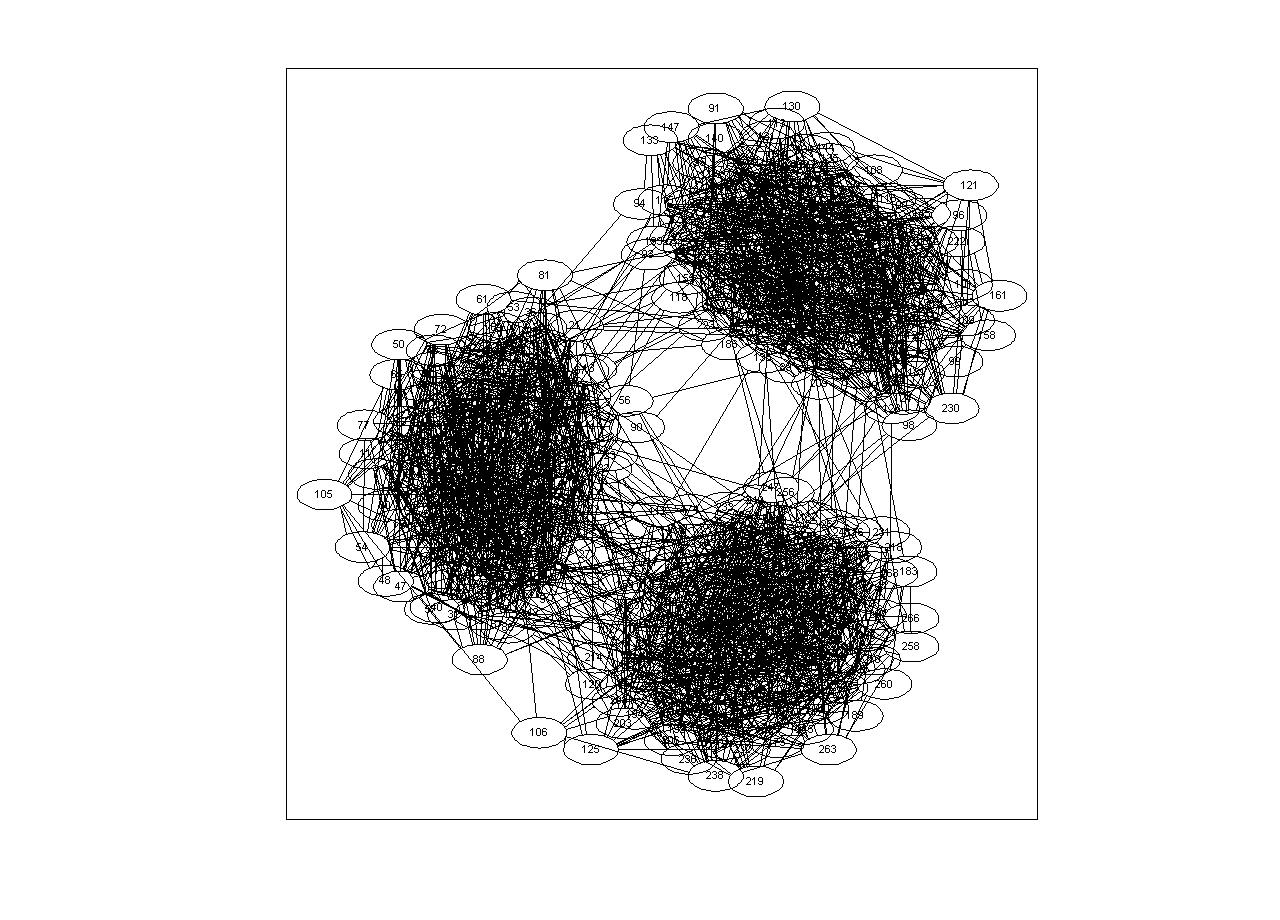
\includegraphics[width=5.0cm,height=5.0cm]{images/3Inhomog_Cluster_PreScaleFree.jpg}   &
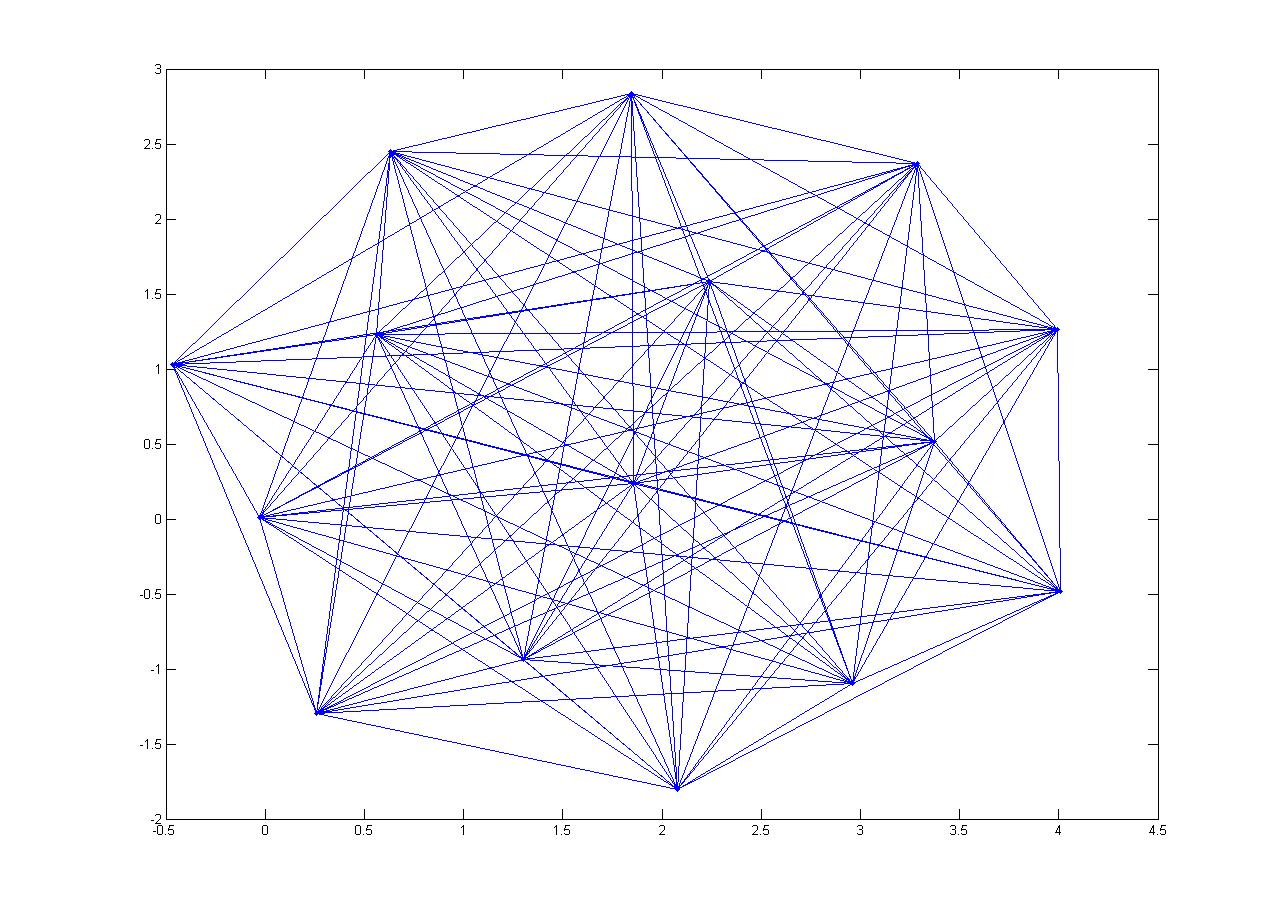
\includegraphics[width=5.0cm,height=5.0cm]{images/Clique_12_Members.jpg}               &
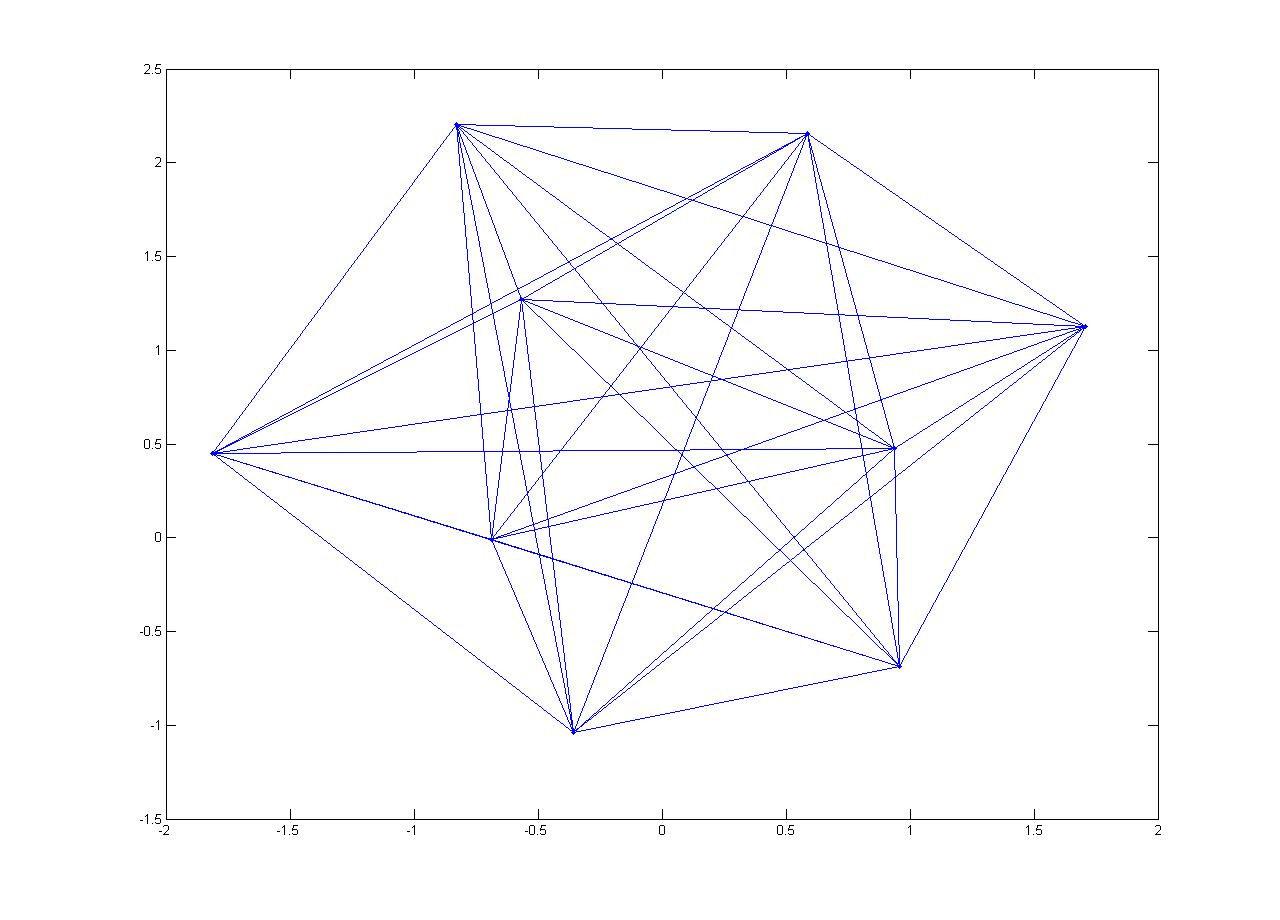
\includegraphics[width=5.0cm,height=5.0cm]{images/Clique_9_Members.jpg}                 \\
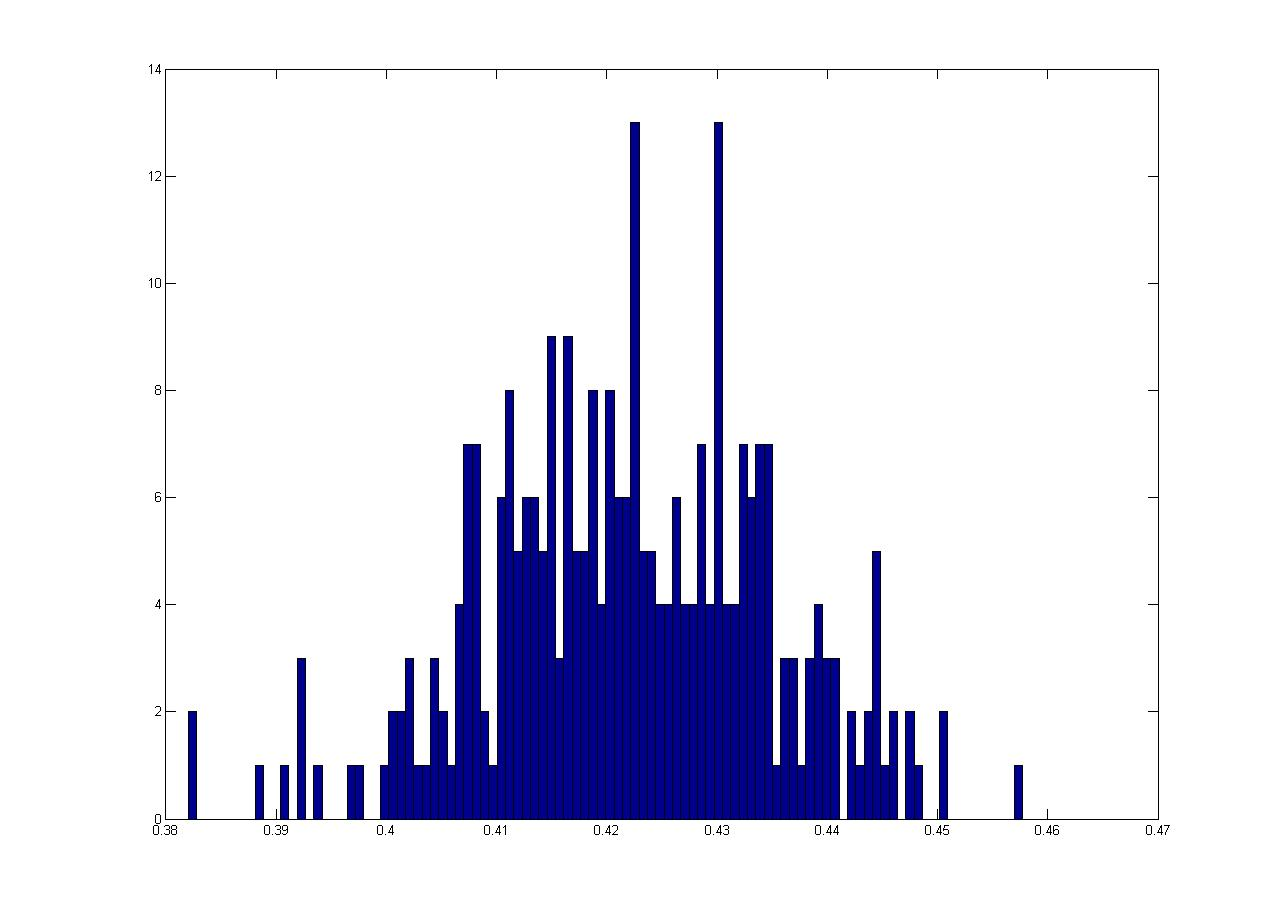
\includegraphics[width=5.0cm,height=5.0cm]{images/ClusterCoeff_Hist_ErdoReyani_Graph_SameVertexSet_mean0_421961099815438.jpg} &
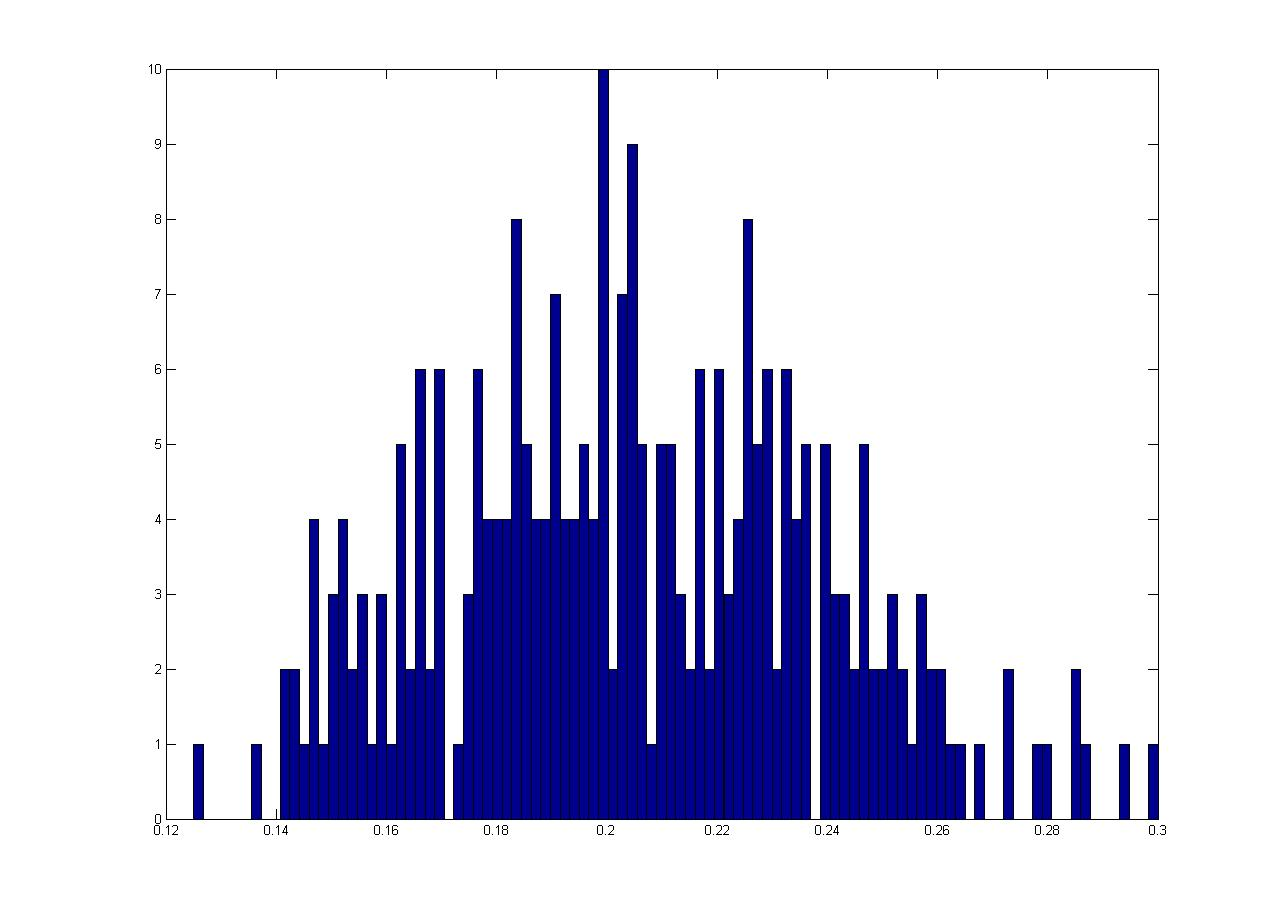
\includegraphics[width=5.0cm,height=5.0cm]{images/ClusterCoeff_Hist_PreScaleFree_mean_0_205047904366710.jpg}                   &
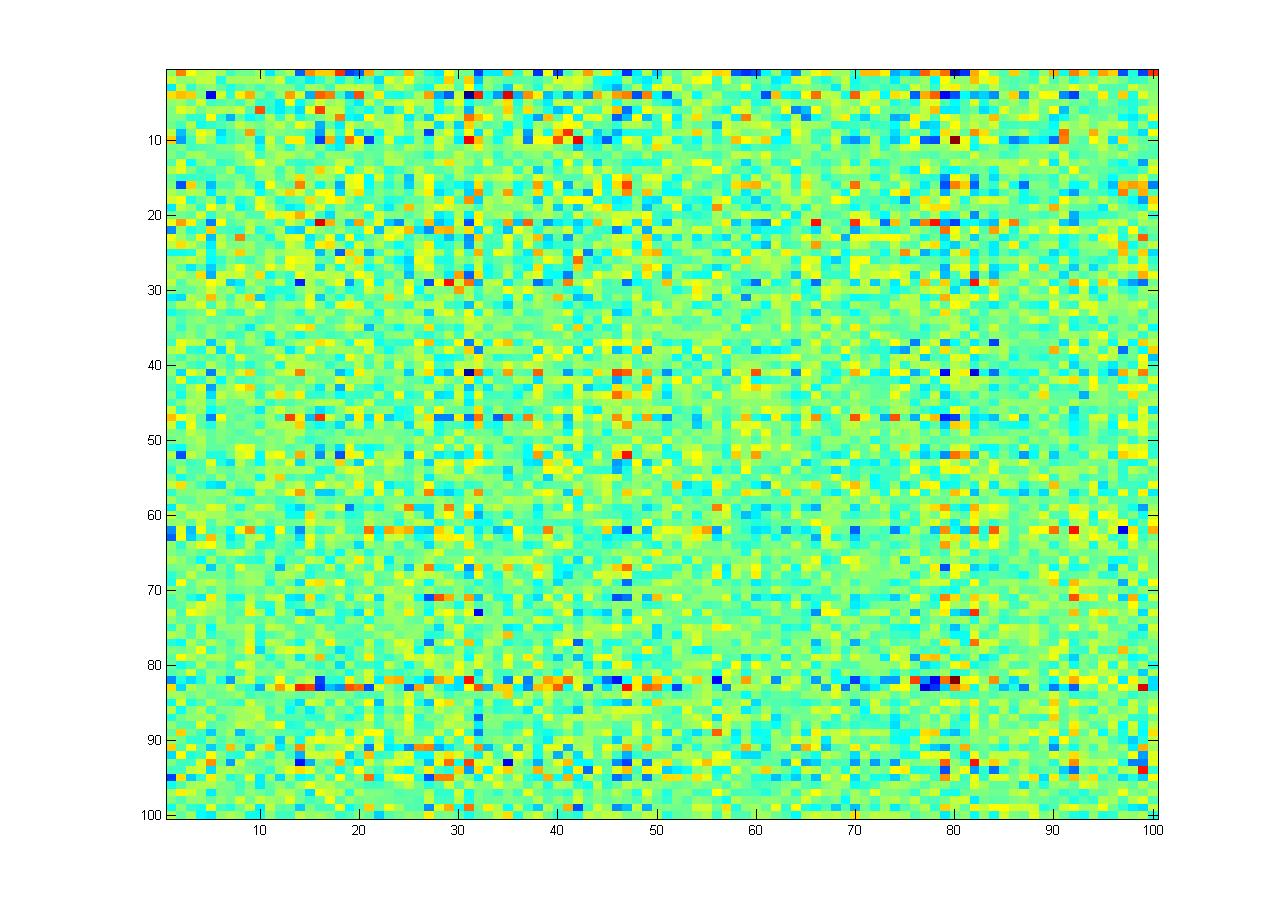
\includegraphics[width=5.0cm,height=5.0cm]{images/CVX_NNMF_A-YX_Where_Y_X_PSD.jpg}                                               \\
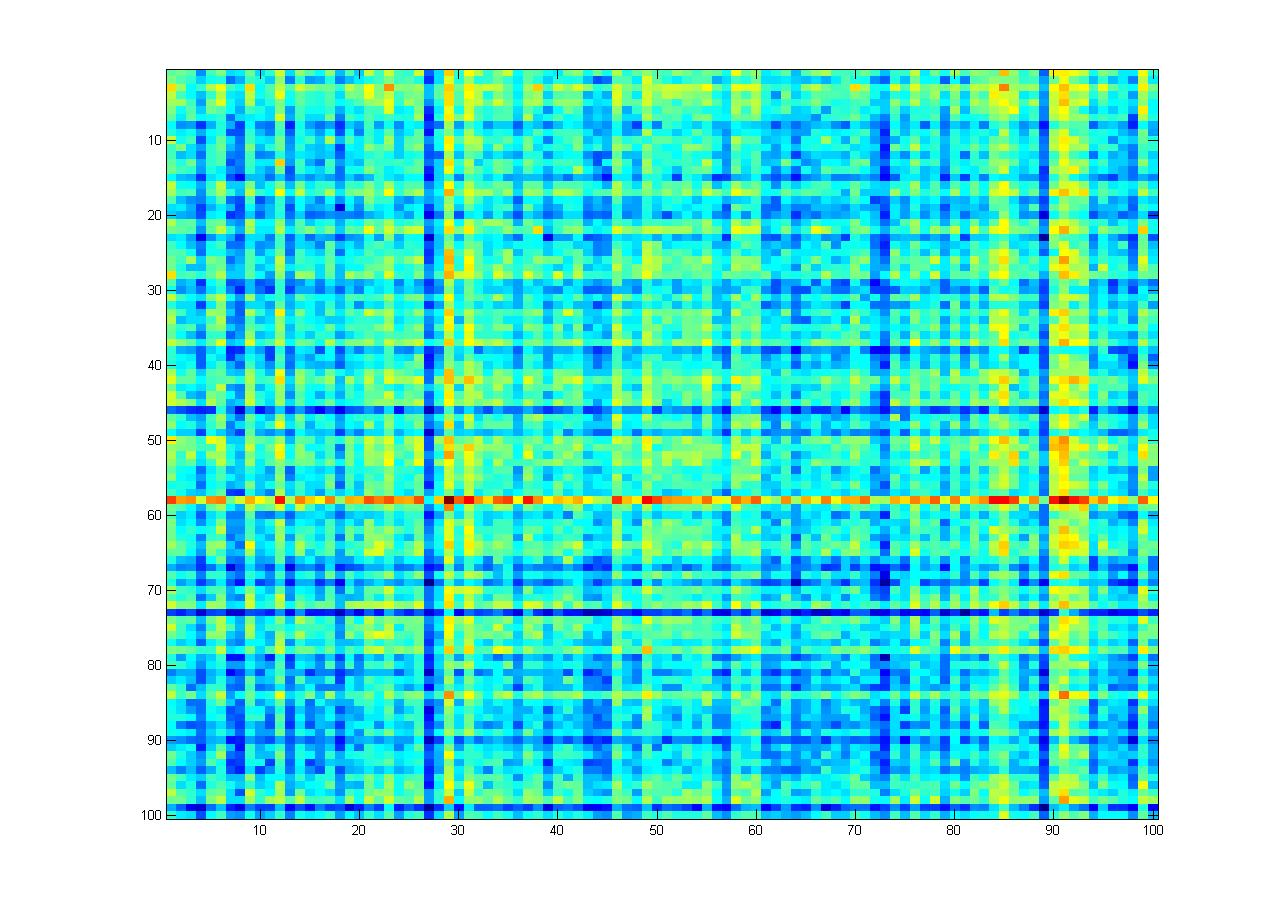
\includegraphics[width=5.0cm,height=5.0cm]{images/CVX_NNMF_A.jpg}                                                                  &
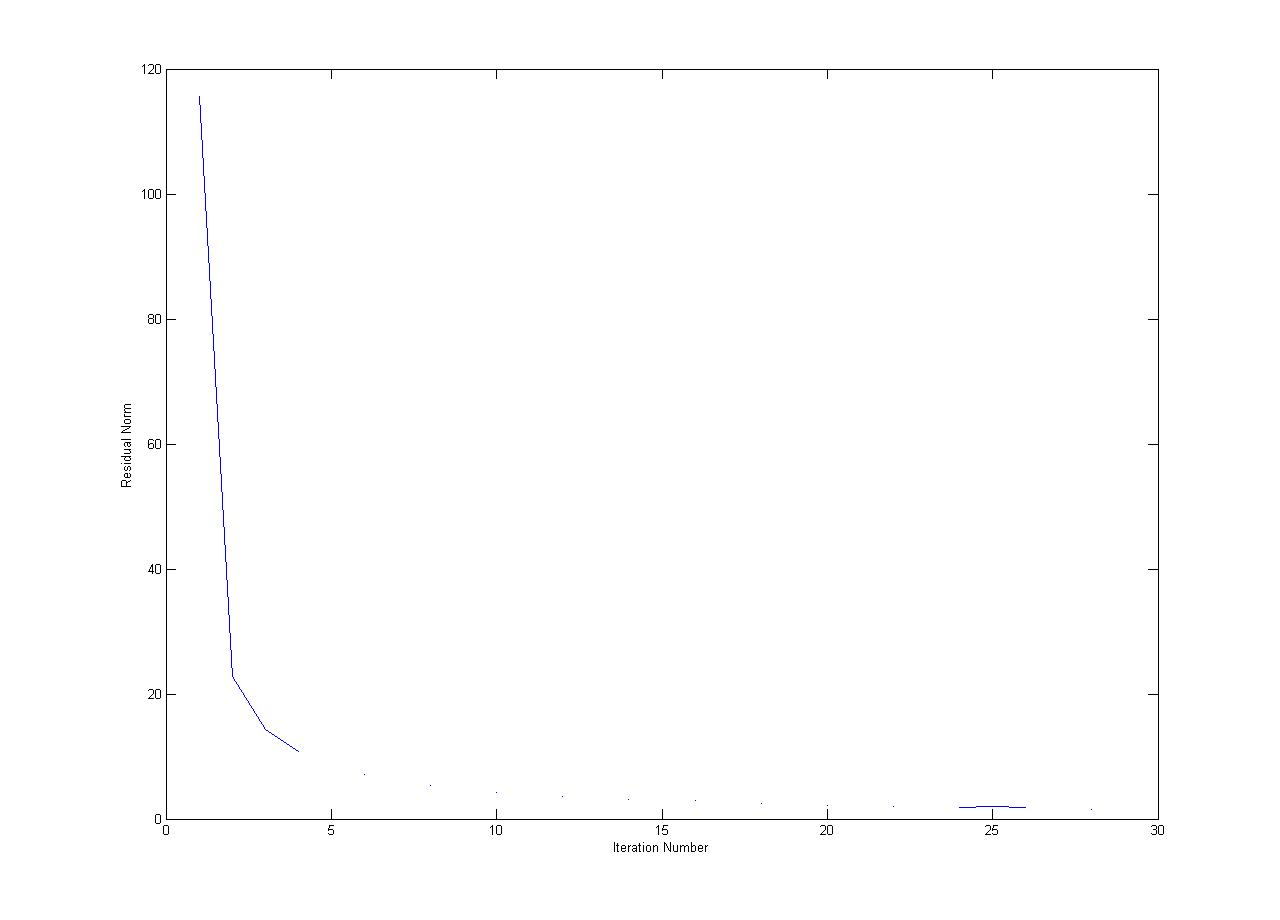
\includegraphics[width=5.0cm,height=5.0cm]{images/CVX_NNMF_Residuals.jpg}                                                           &
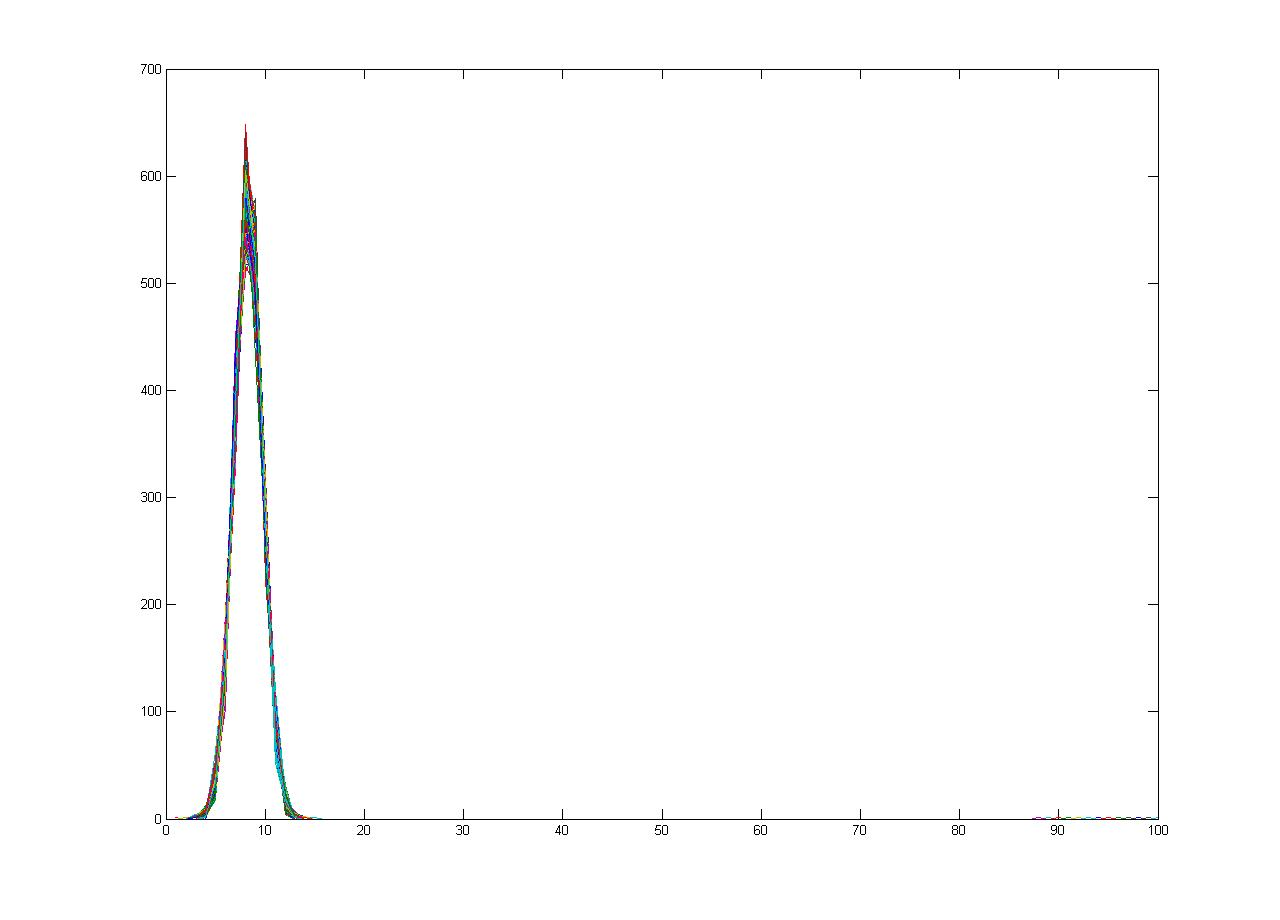
\includegraphics[width=5.0cm,height=5.0cm]{images/Eigenvalues_of_Whshart_Follow_TracyWidom.jpg}             \\
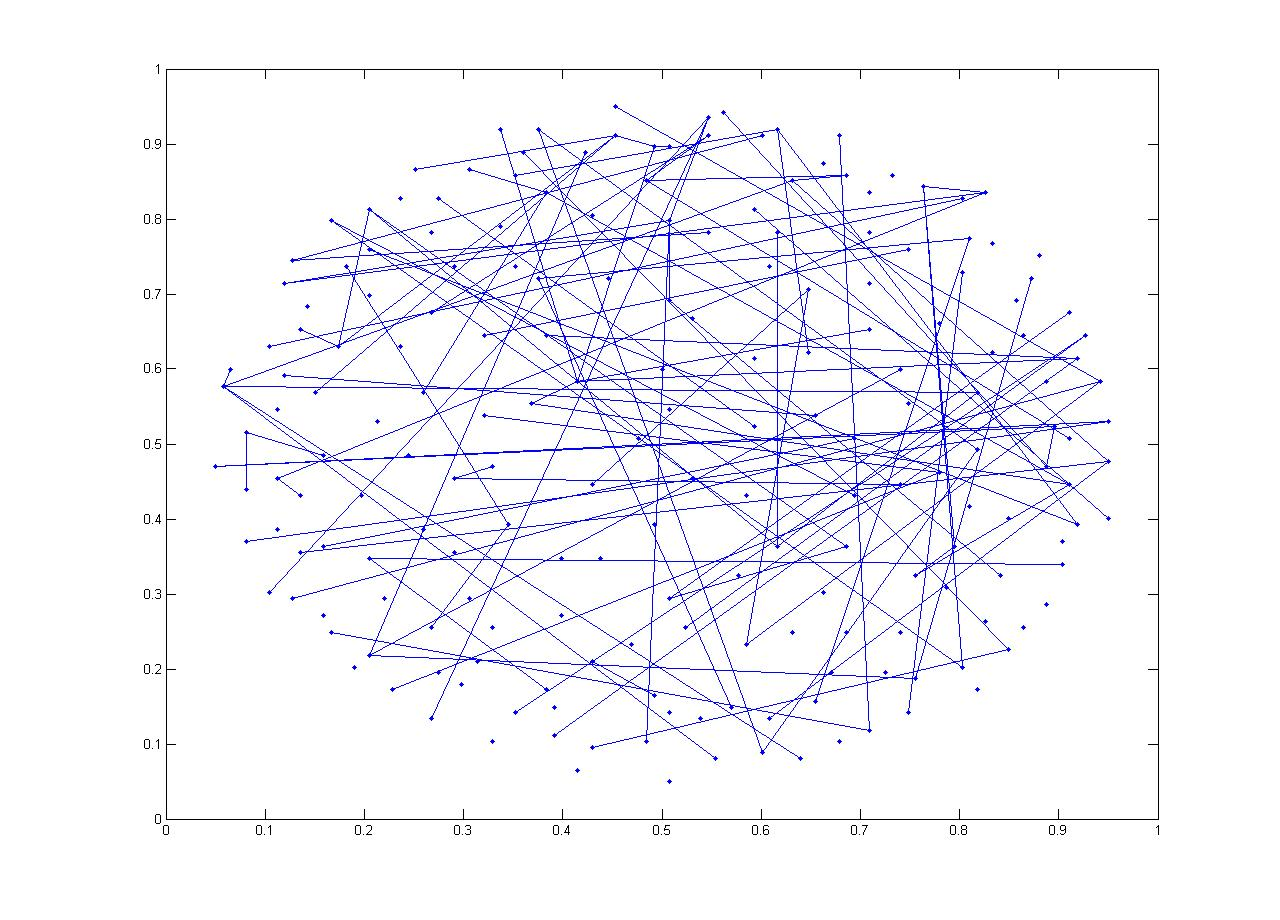
\includegraphics[width=5.0cm,height=5.0cm]{images/ErdosReyni_G_LT_giant_thresh_.jpg}         &
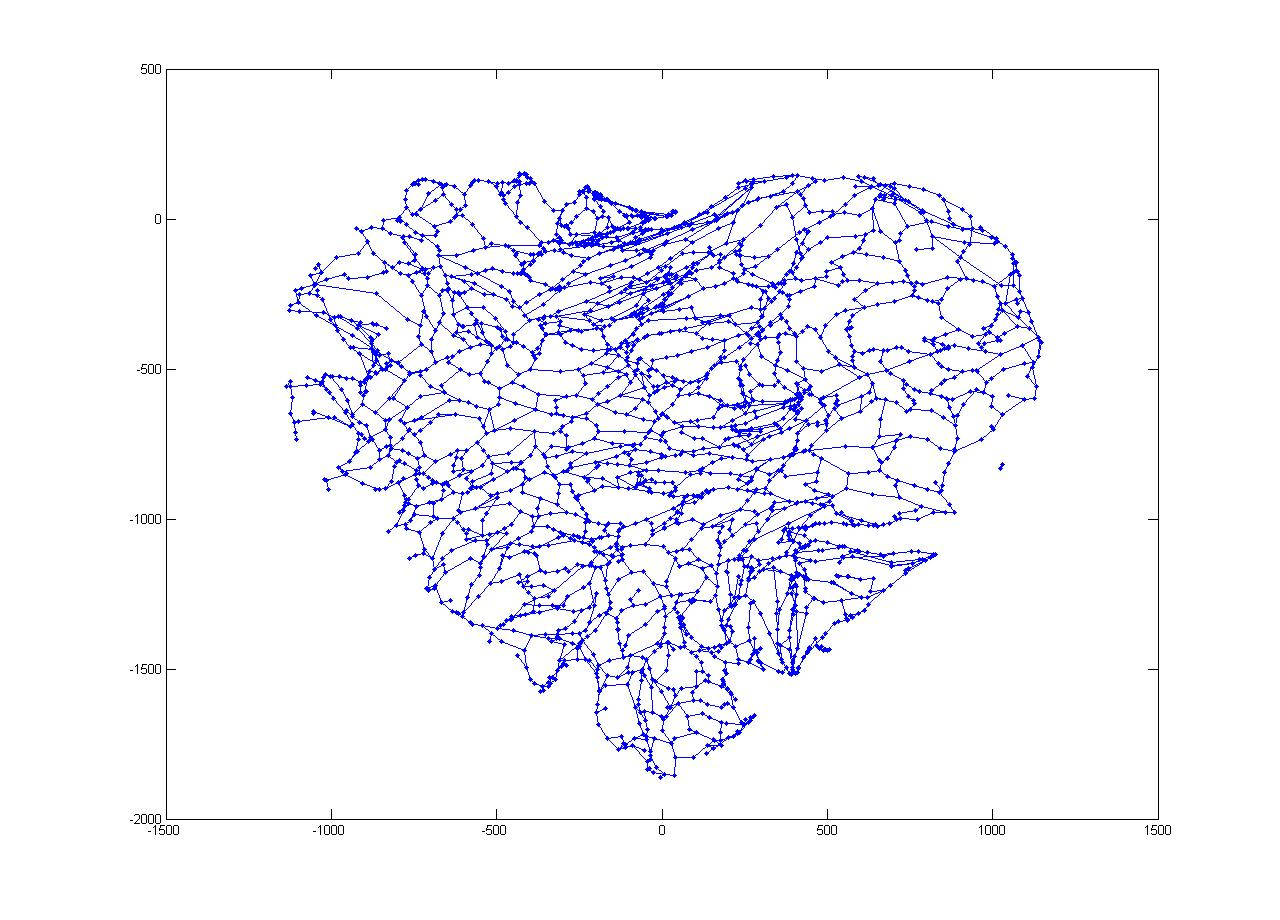
\includegraphics[width=5.0cm,height=5.0cm]{images/gursoy_atun_layou_topology_heart.jpg}       &
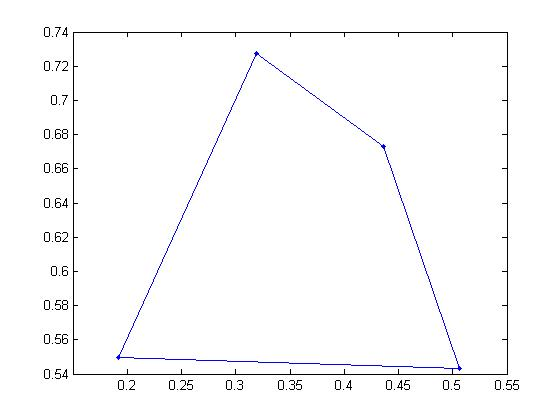
\includegraphics[width=5.0cm,height=5.0cm]{images/hypercube_3_Dimension.jpg}
\end{tabular}

\begin{tabular}{ |c|c|c| }
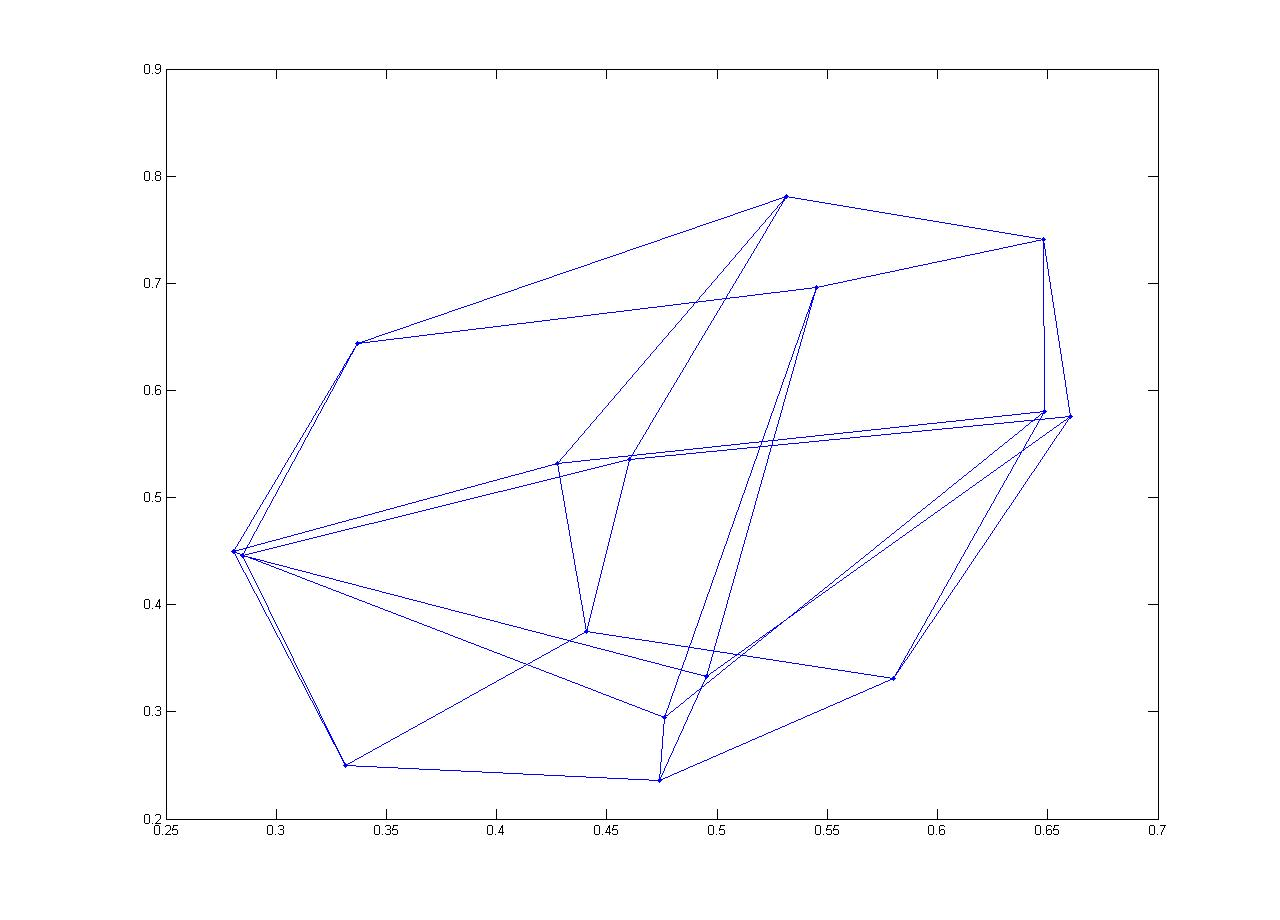
\includegraphics[width=5.0cm,height=5.0cm]{images/hypercube_4_Dimension.jpg}  &
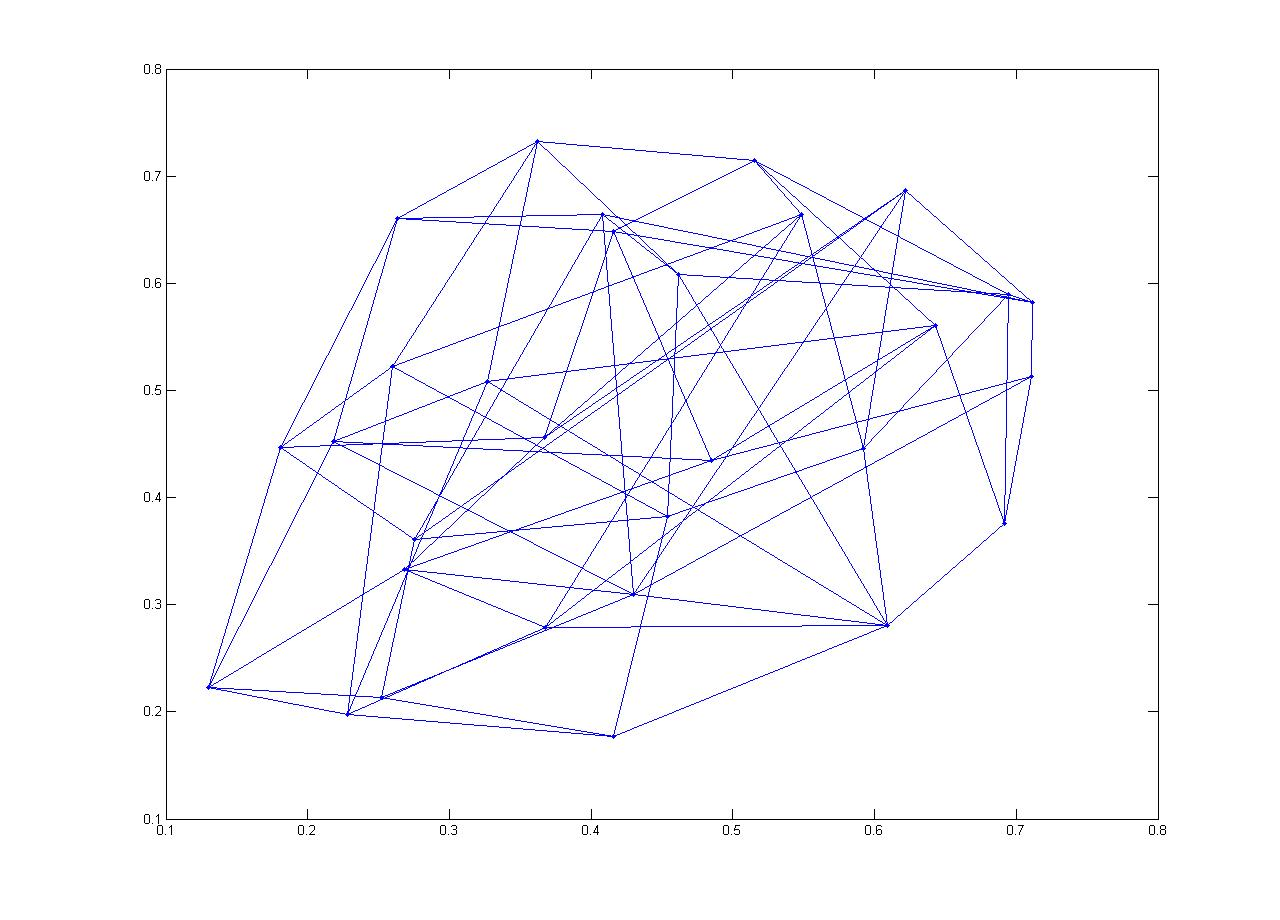
\includegraphics[width=5.0cm,height=5.0cm]{images/hypercube_5_Dimension.jpg}   &
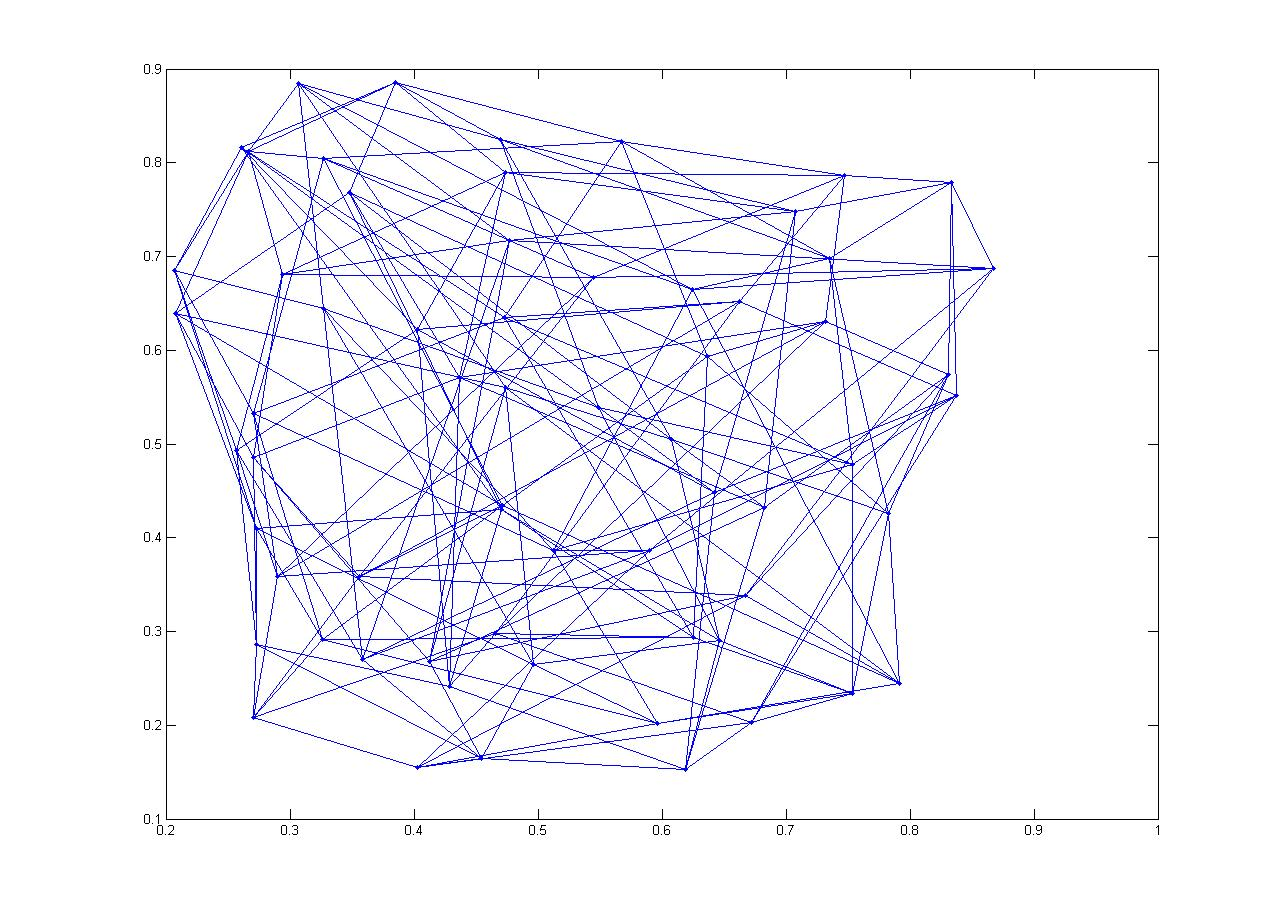
\includegraphics[width=5.0cm,height=5.0cm]{images/hypercube_6_Dimension.jpg}    \\
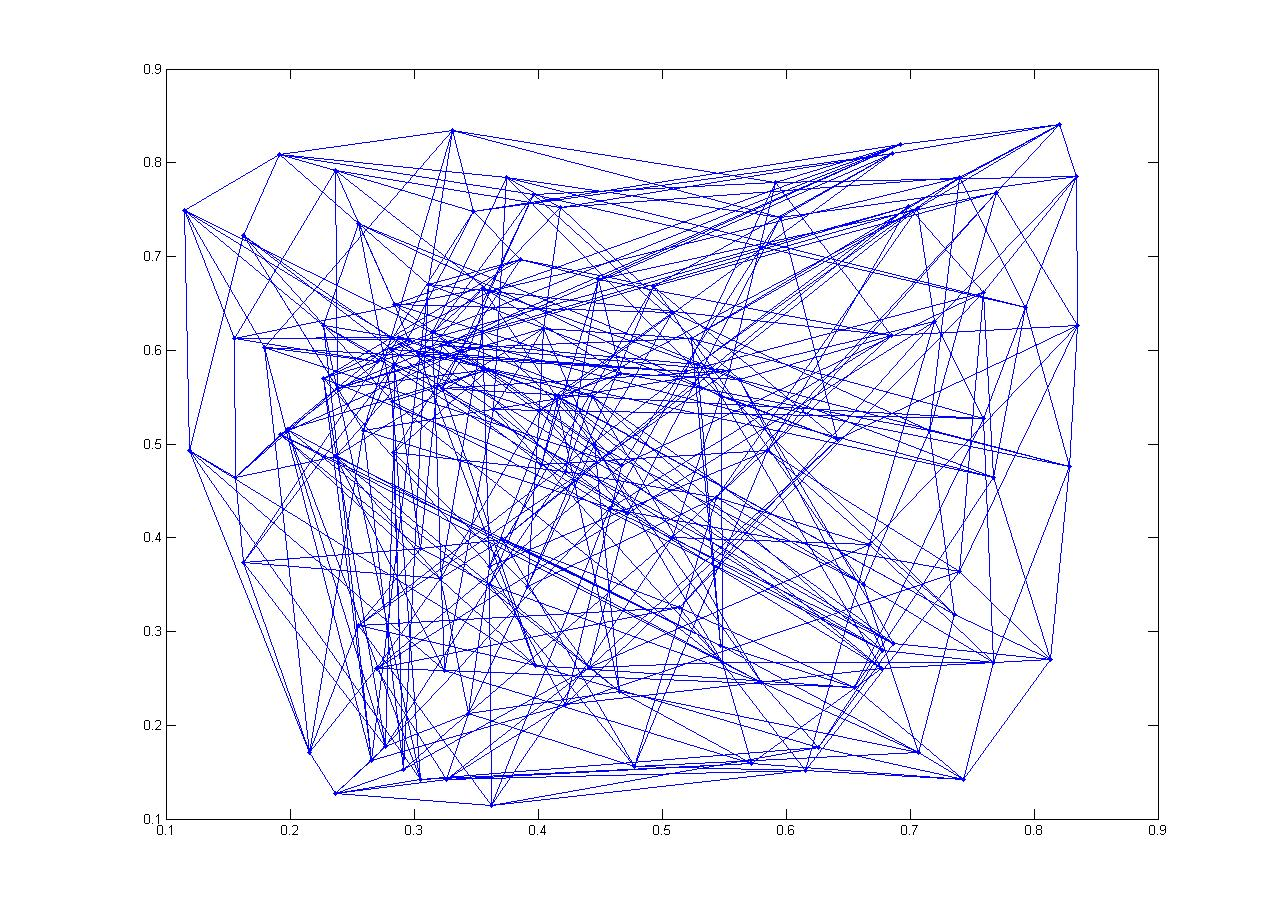
\includegraphics[width=5.0cm,height=5.0cm]{images/hypercube_7_Dimension.jpg}      &
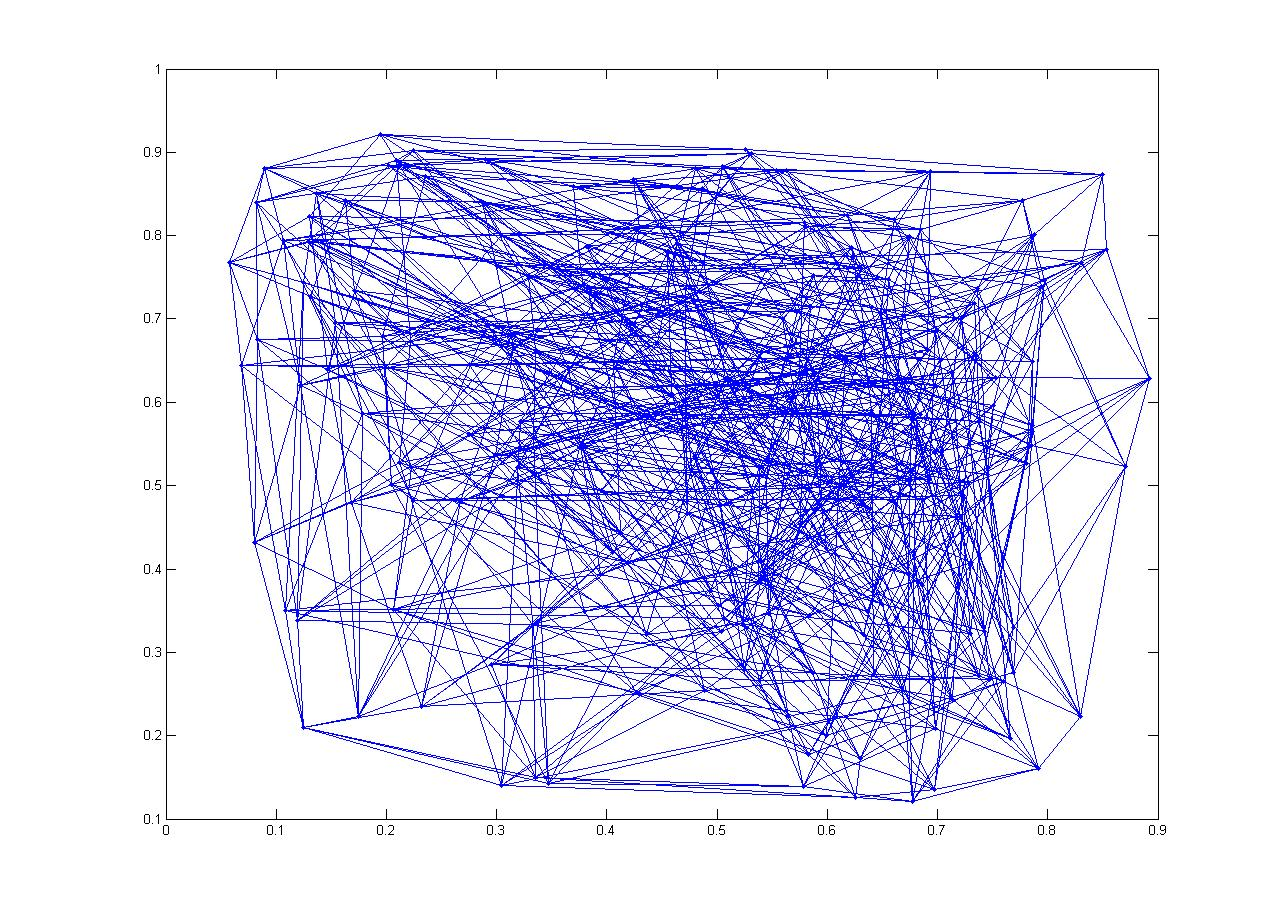
\includegraphics[width=5.0cm,height=5.0cm]{images/hypercube_8_Dimension.jpg}       &
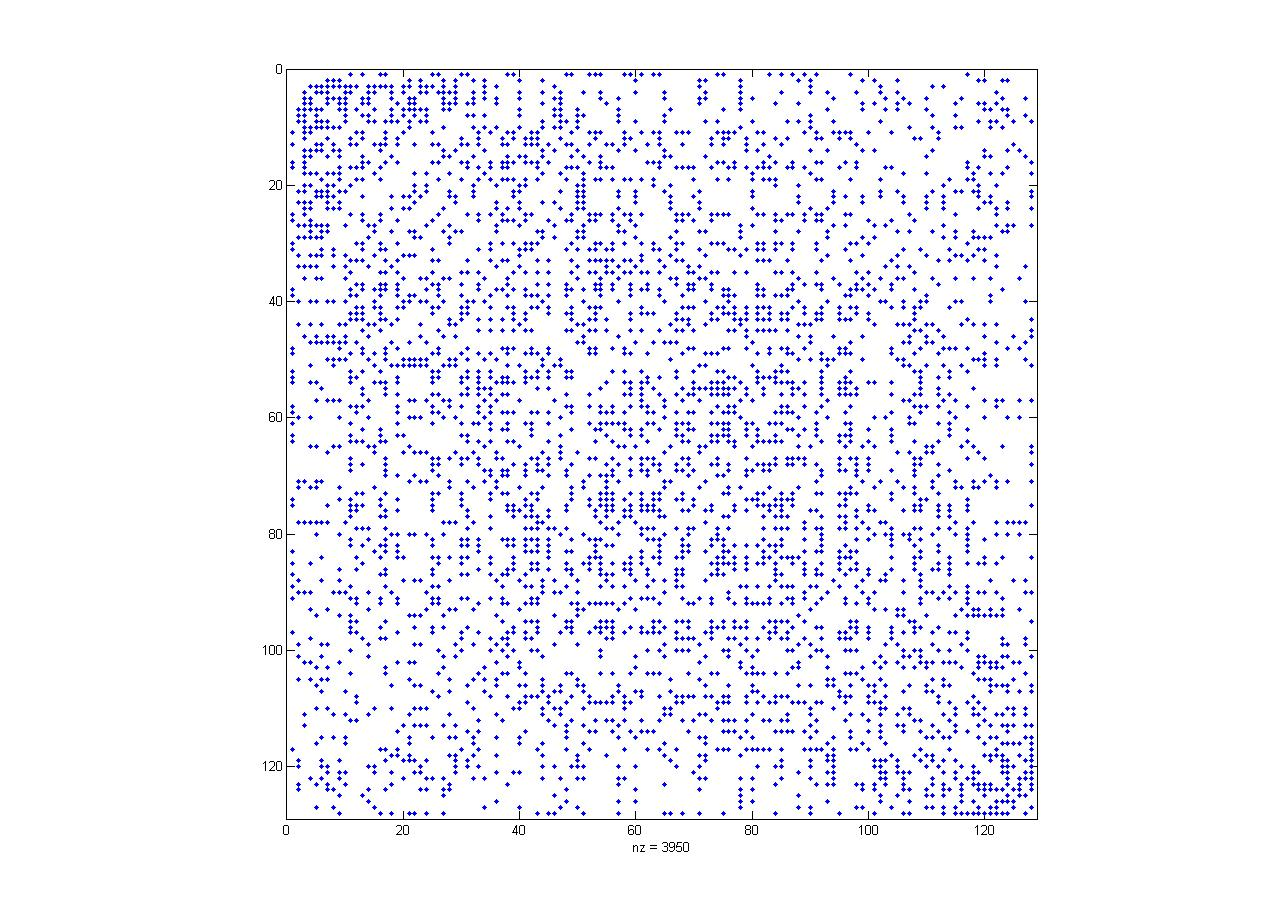
\includegraphics[width=5.0cm,height=5.0cm]{images/RandomGraphAdjacencyMatrix_WithCut_jpg.jpg} \\
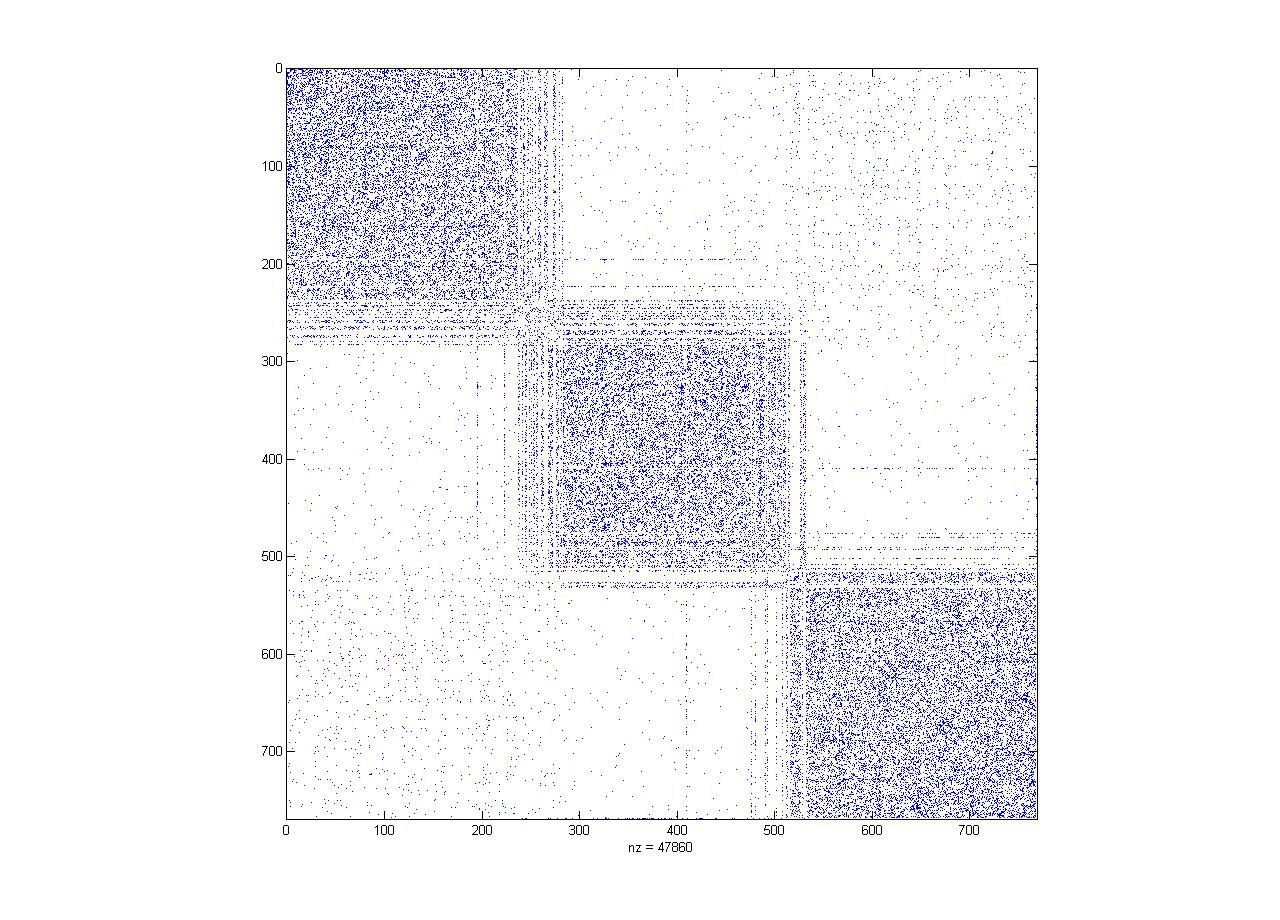
\includegraphics[width=5.0cm,height=5.0cm]{images/RandomGraphOptimalEdgeInputGraph_256_Nodes_AdjacencyMatrix.jpg} &
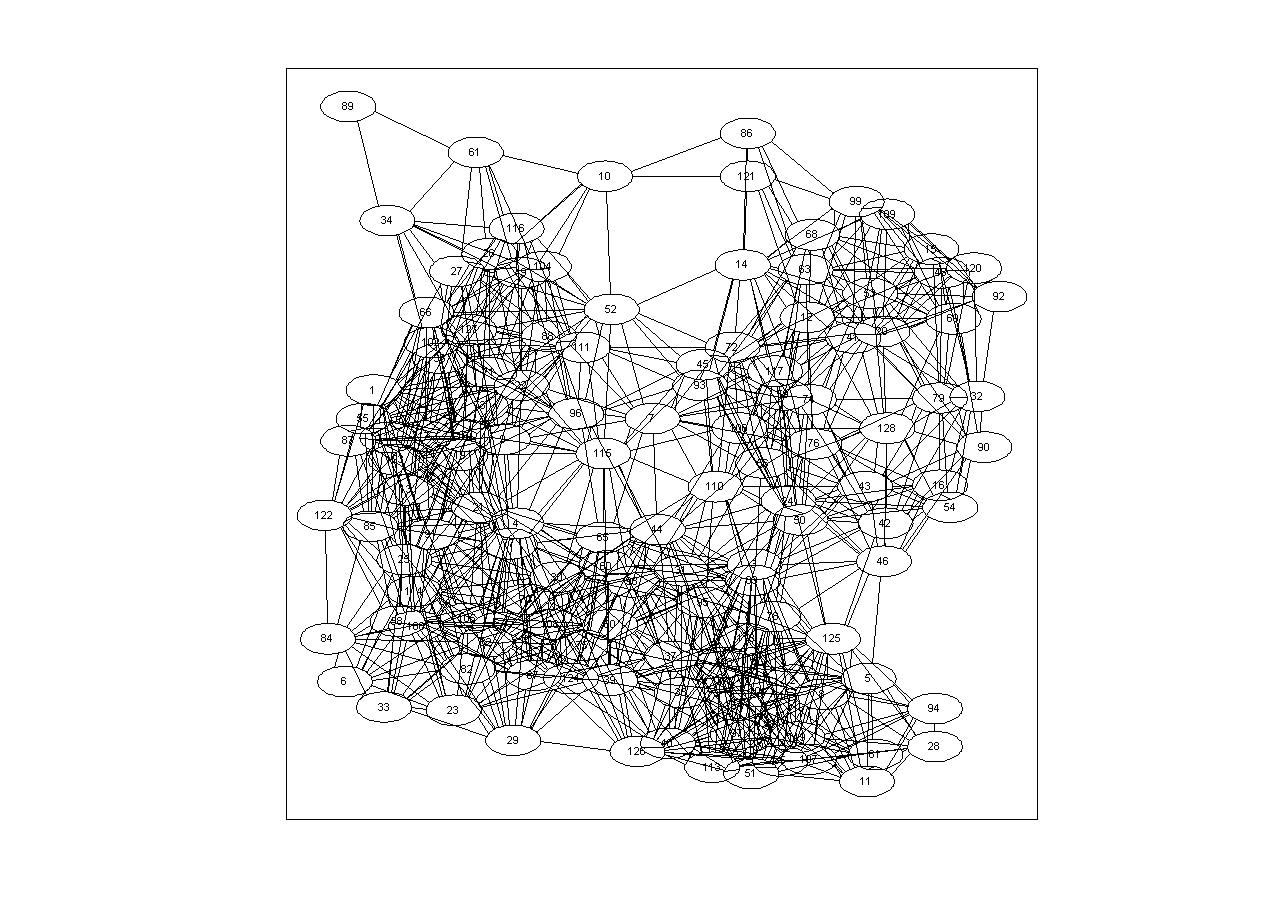
\includegraphics[width=5.0cm,height=5.0cm]{images/RandomGraphOptimalEdgeInputGraph_AdjacencyMatrix.jpg}            &
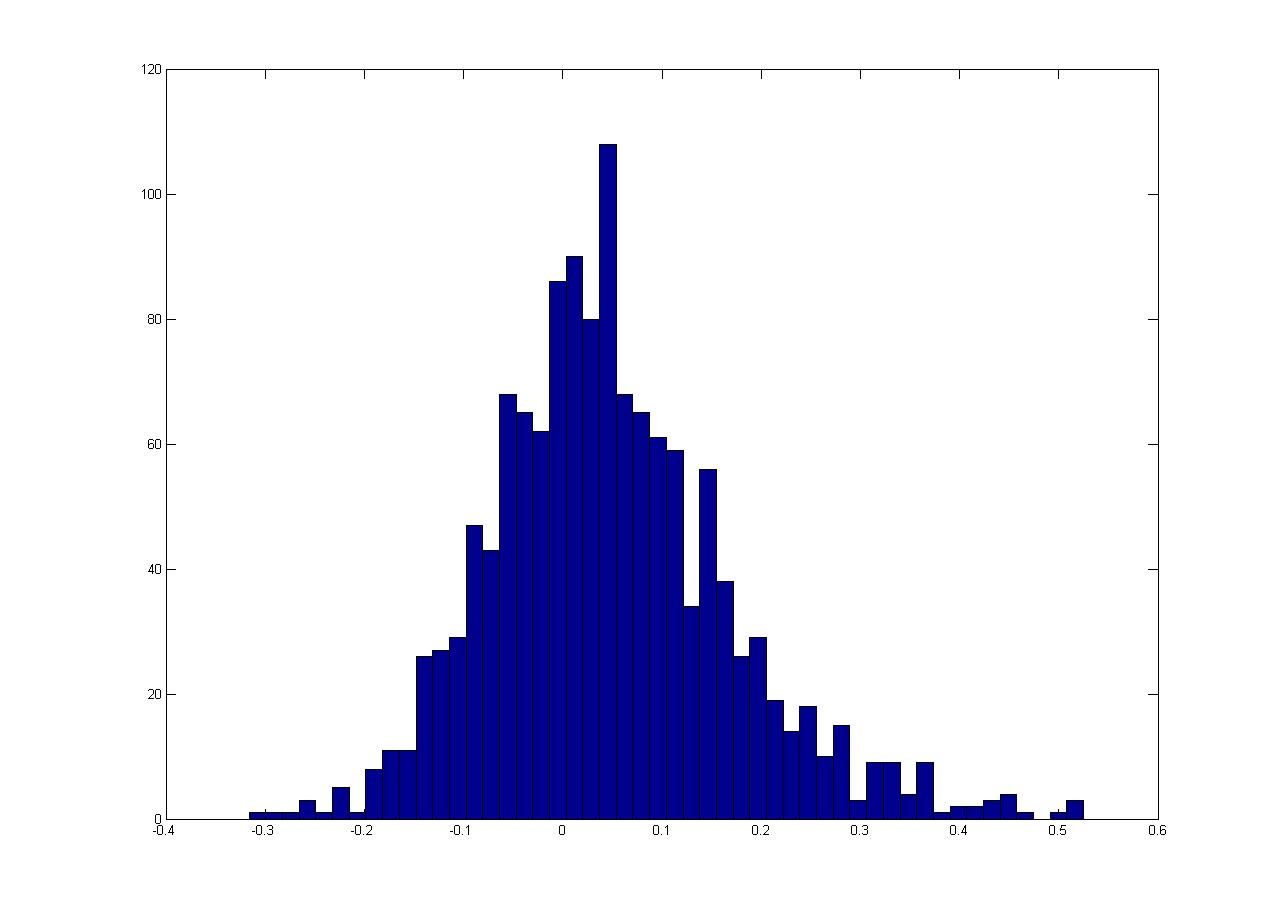
\includegraphics[width=5.0cm,height=5.0cm]{images/RandomGraphOptimalEdgeInputGraph_EdgeWeightHist_FMMC.jpg}         \\
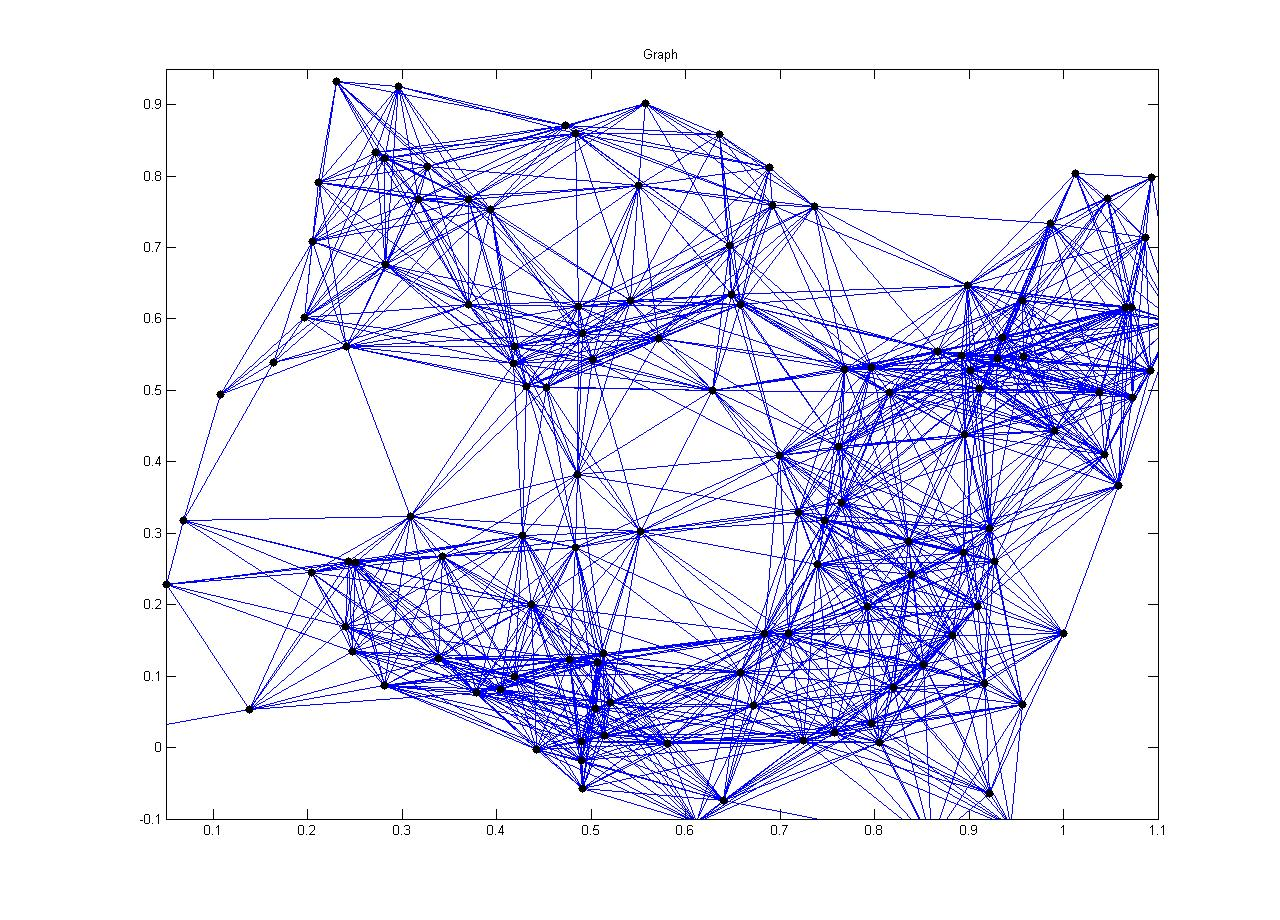
\includegraphics[width=5.0cm,height=5.0cm]{images/RandomGraphOptimalEdgeInputGraph_IncidenceMatrix.jpg}               &
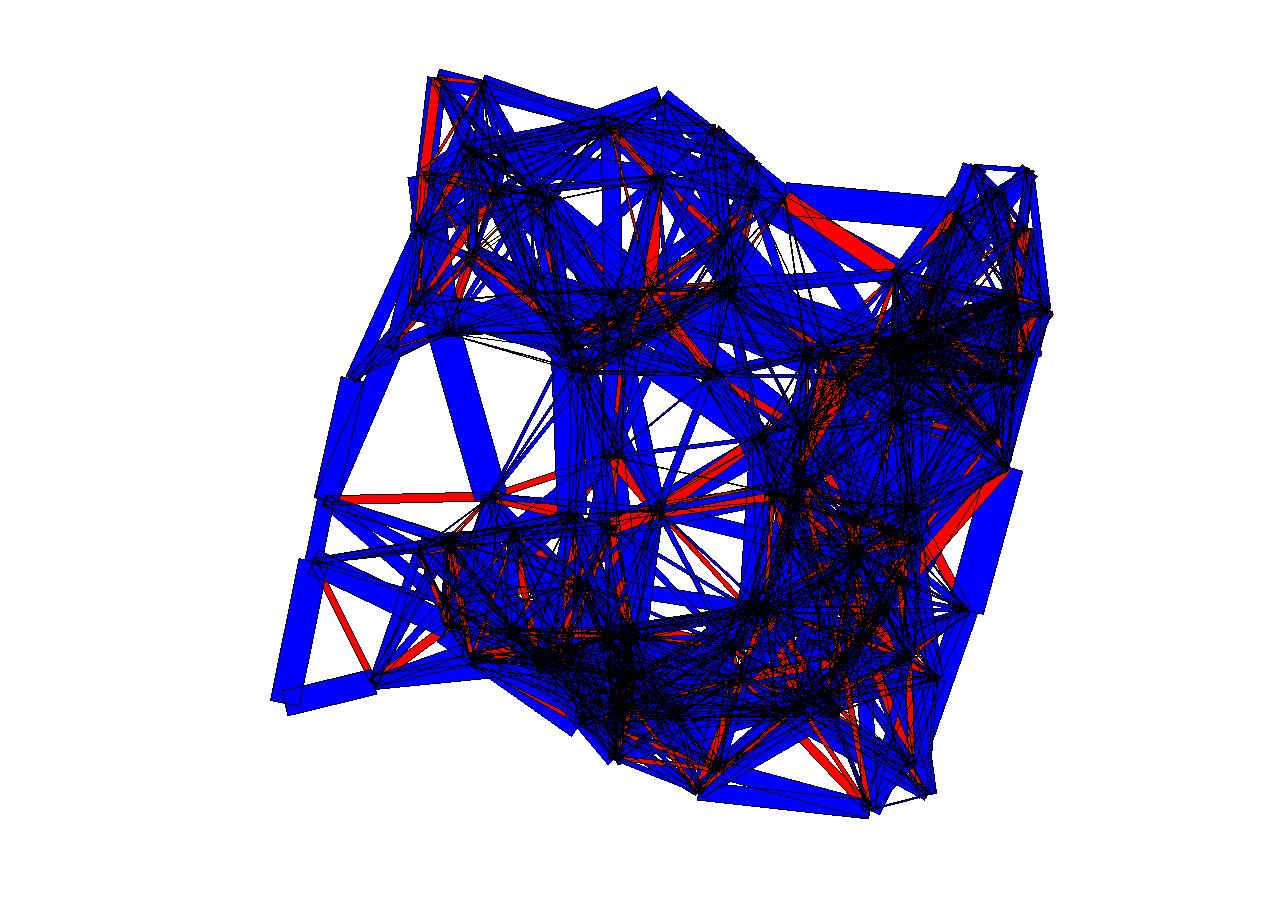
\includegraphics[width=5.0cm,height=5.0cm]{images/RandomGraphOptimalEdgeWithedgeWeight_FastMixingMarkovChain.jpg}      &
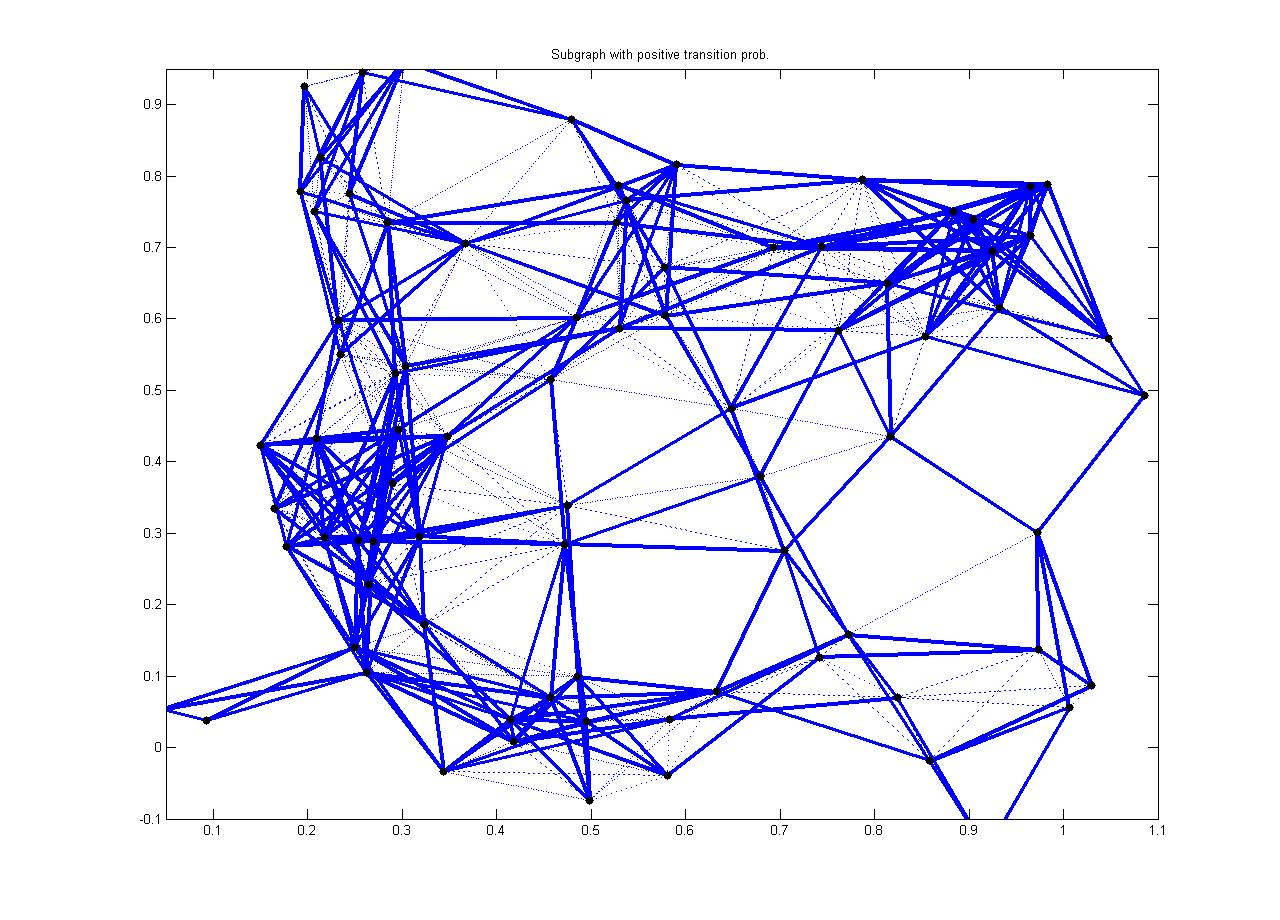
\includegraphics[width=5.0cm,height=5.0cm]{images/RandomGraphOptimalEdgeWithedgeWeight_PositiveTransitionProbs_FastMixingMarkovChain.jpg}
\end{tabular}

\begin{tabular}{ |c|c|c| }
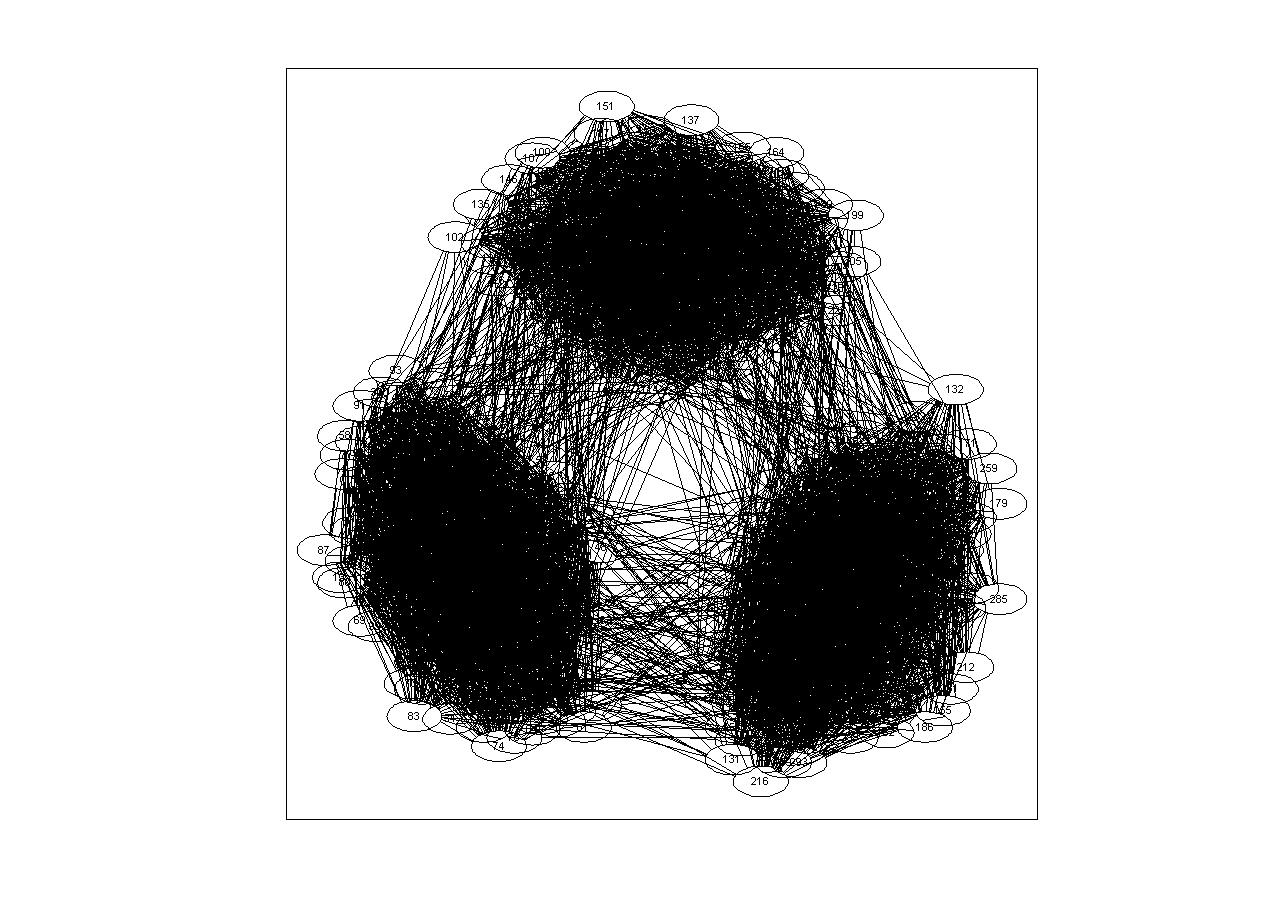
\includegraphics[width=5.0cm,height=5.0cm]{images/RandomGraph_With3Cuts_.jpg}                                               &
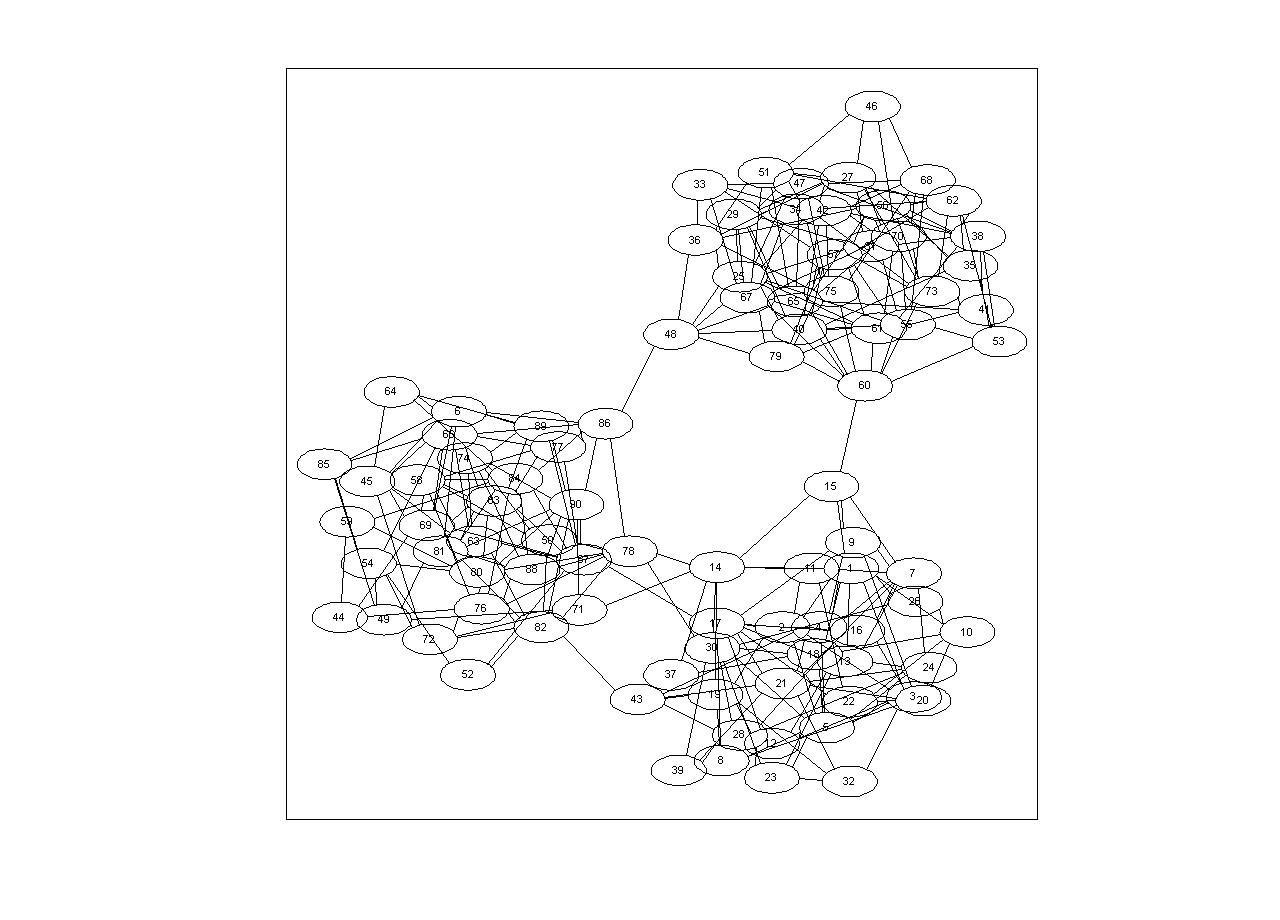
\includegraphics[width=5.0cm,height=5.0cm]{images/RandomGraph_With3Cuts_90_nodes_pii_25_pij_06.jpg}                          &
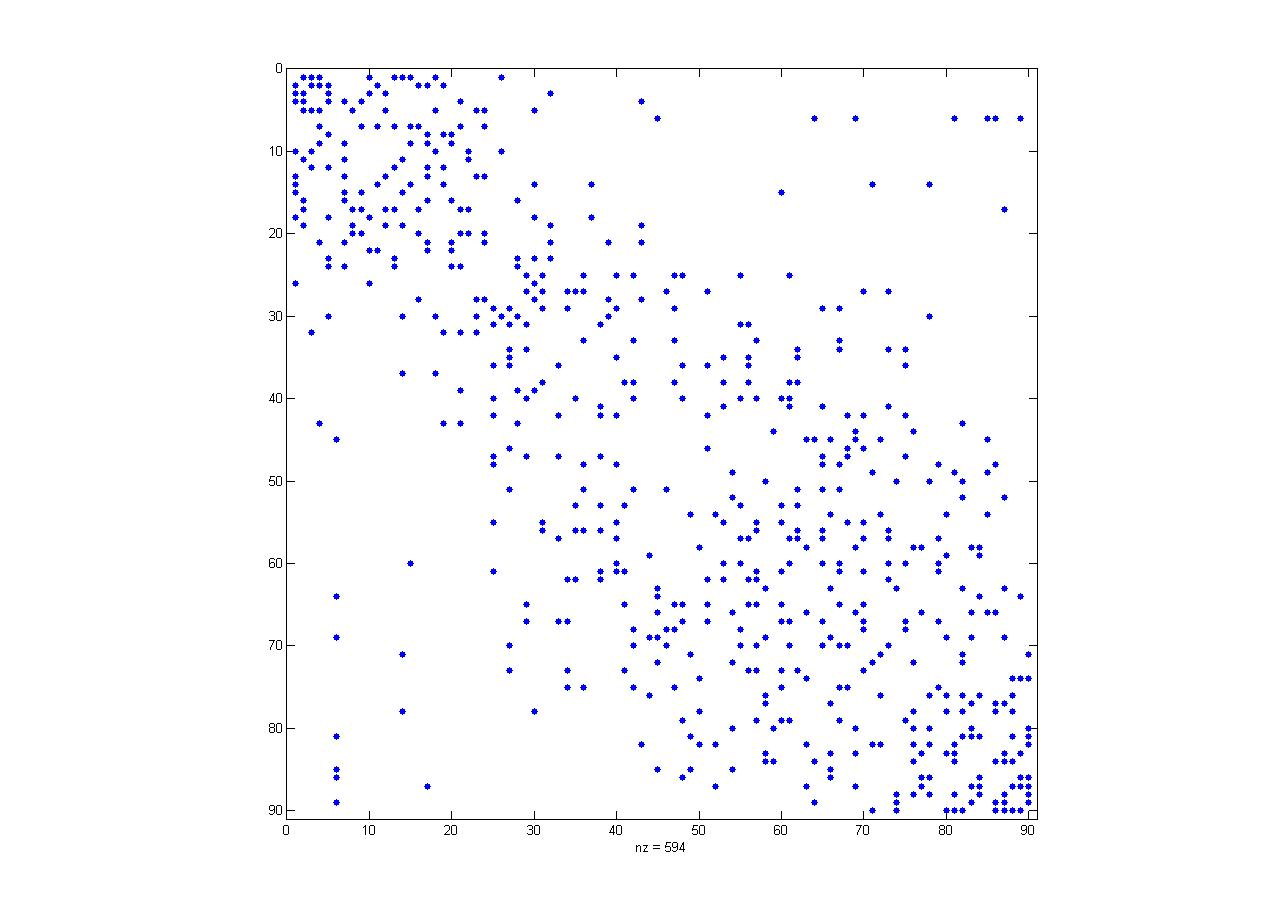
\includegraphics[width=5.0cm,height=5.0cm]{images/RandomGraph_With3Cuts_90_nodes_pii_25_pij_06_Adjacency_Matrix.jpg}          \\
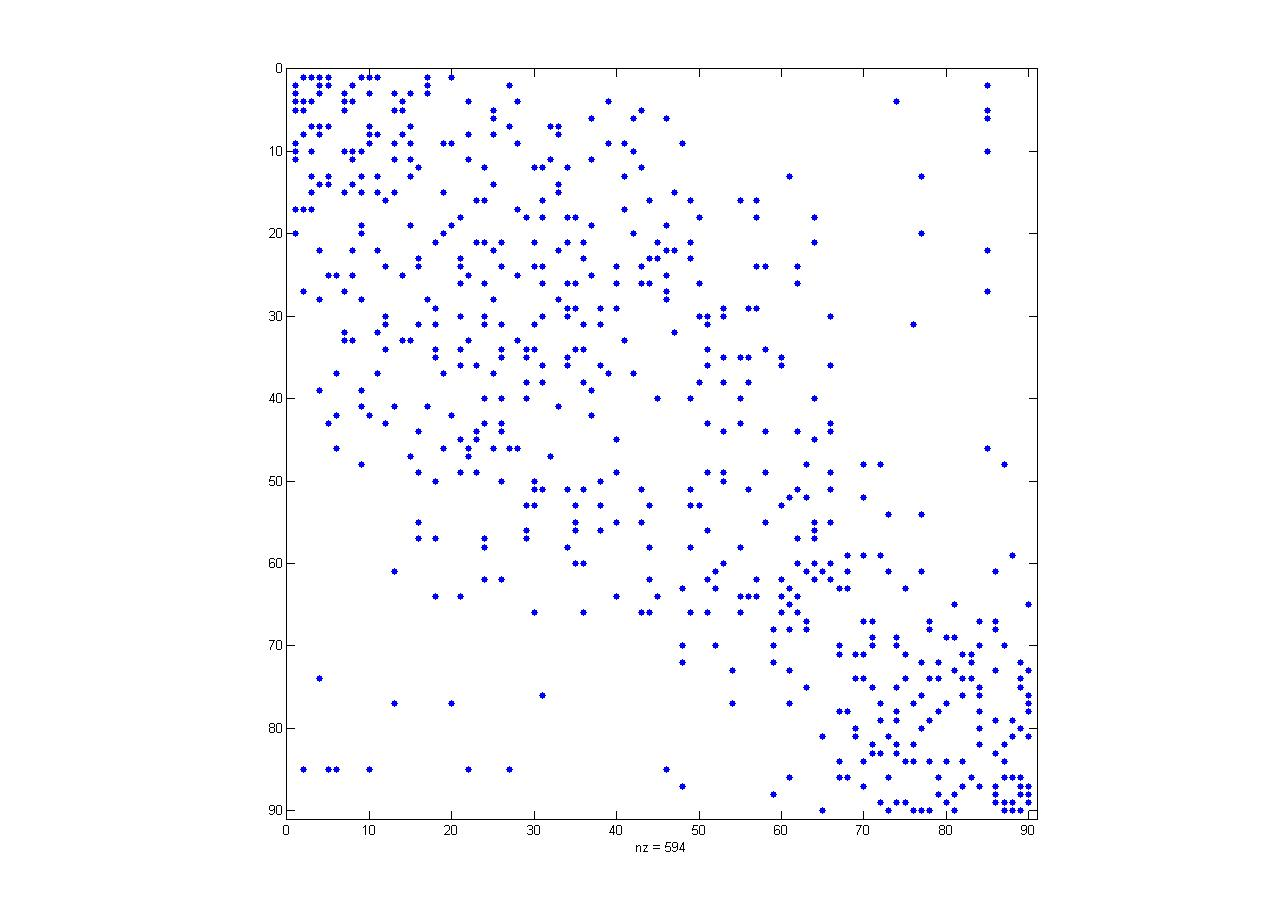
\includegraphics[width=5.0cm,height=5.0cm]{images/RandomGraph_With3Cuts_90_nodes_pii_25_pij_06_Adjacency_Matrix_Minimized_PF.jpg}  &
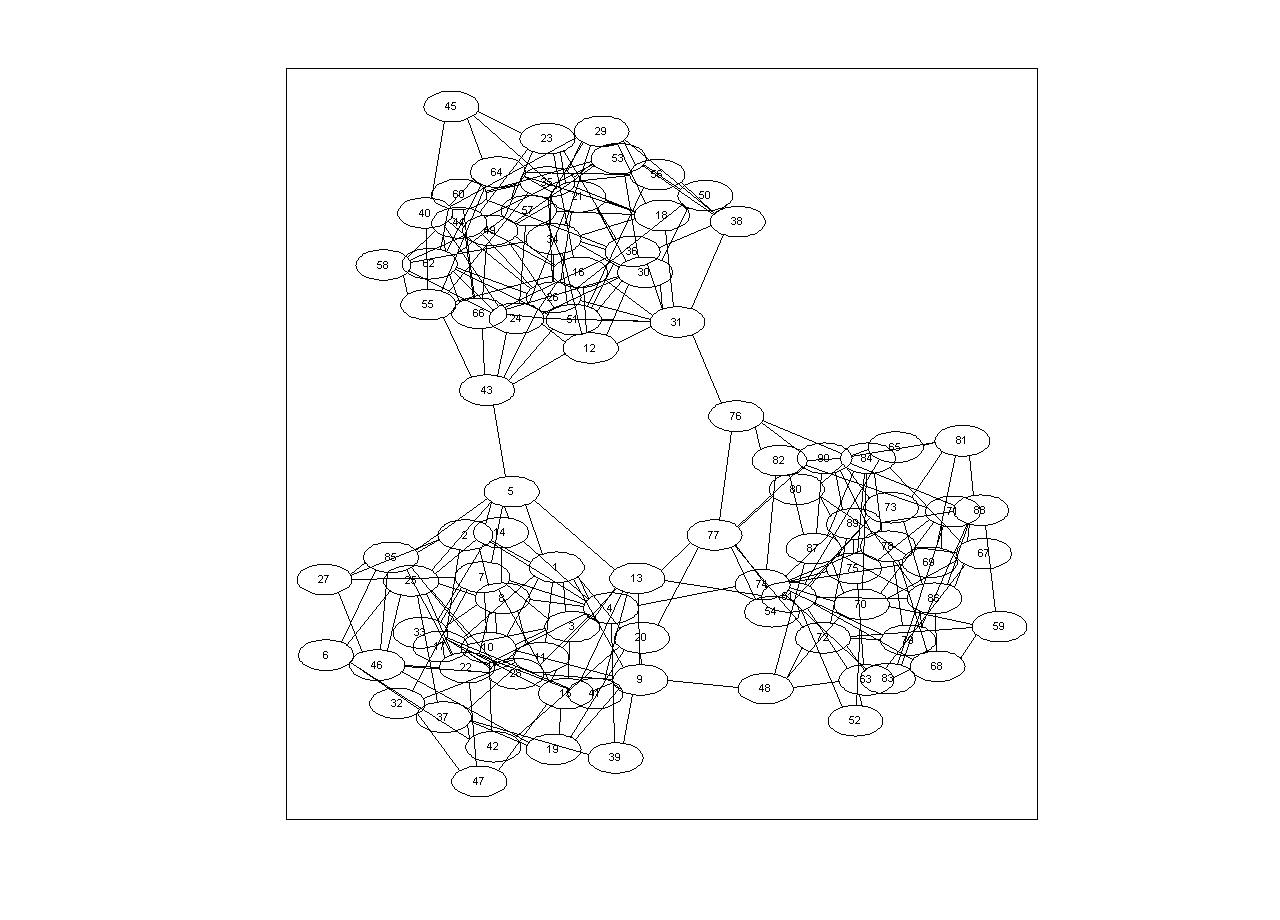
\includegraphics[width=5.0cm,height=5.0cm]{images/RandomGraph_With3Cuts_90_nodes_pii_25_pij_06_MinimizedAdjacency_PerronFrobenius.jpg} &
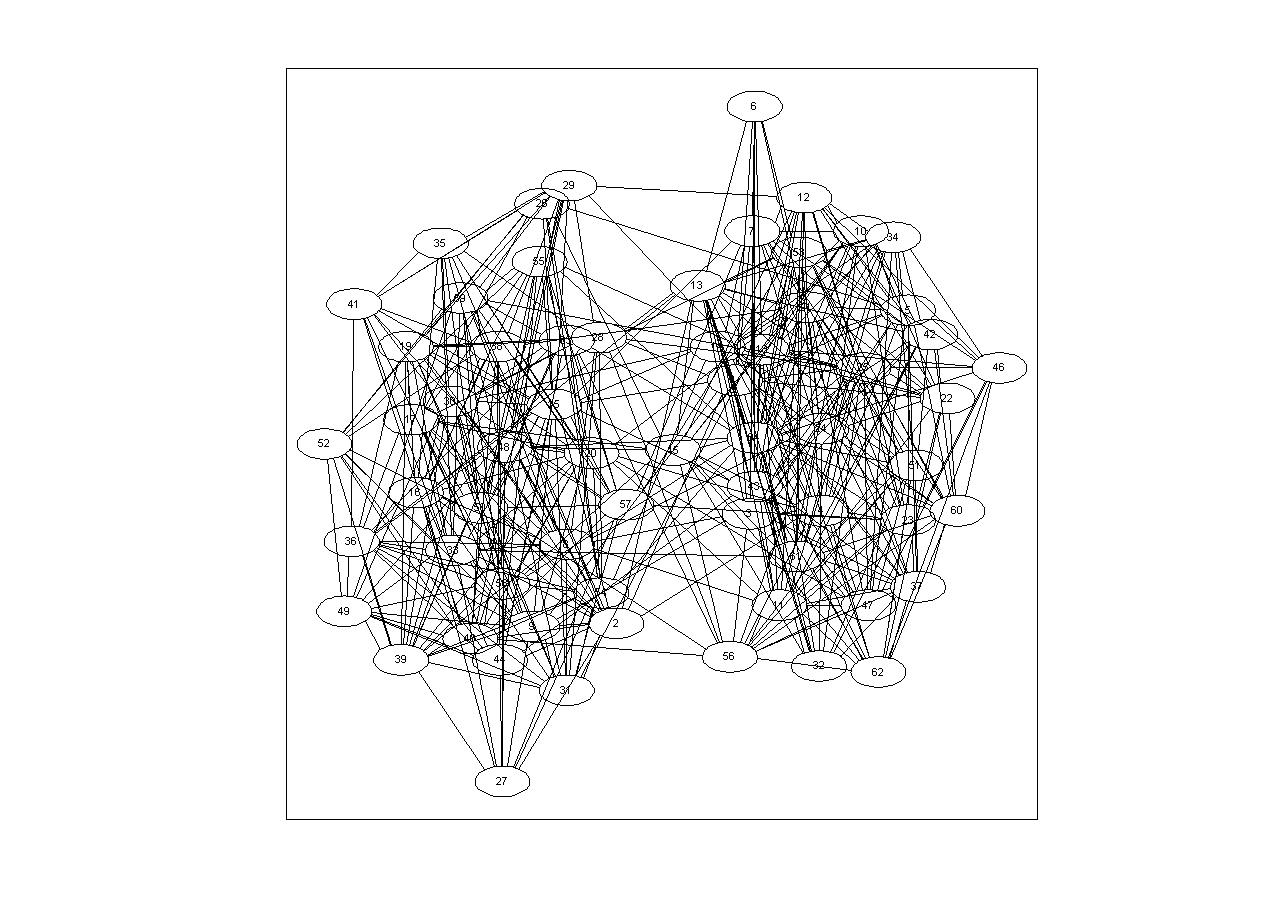
\includegraphics[width=5.0cm,height=5.0cm]{images/RandomGraph_WithCut_64Nodes.jpg}                                                      \\
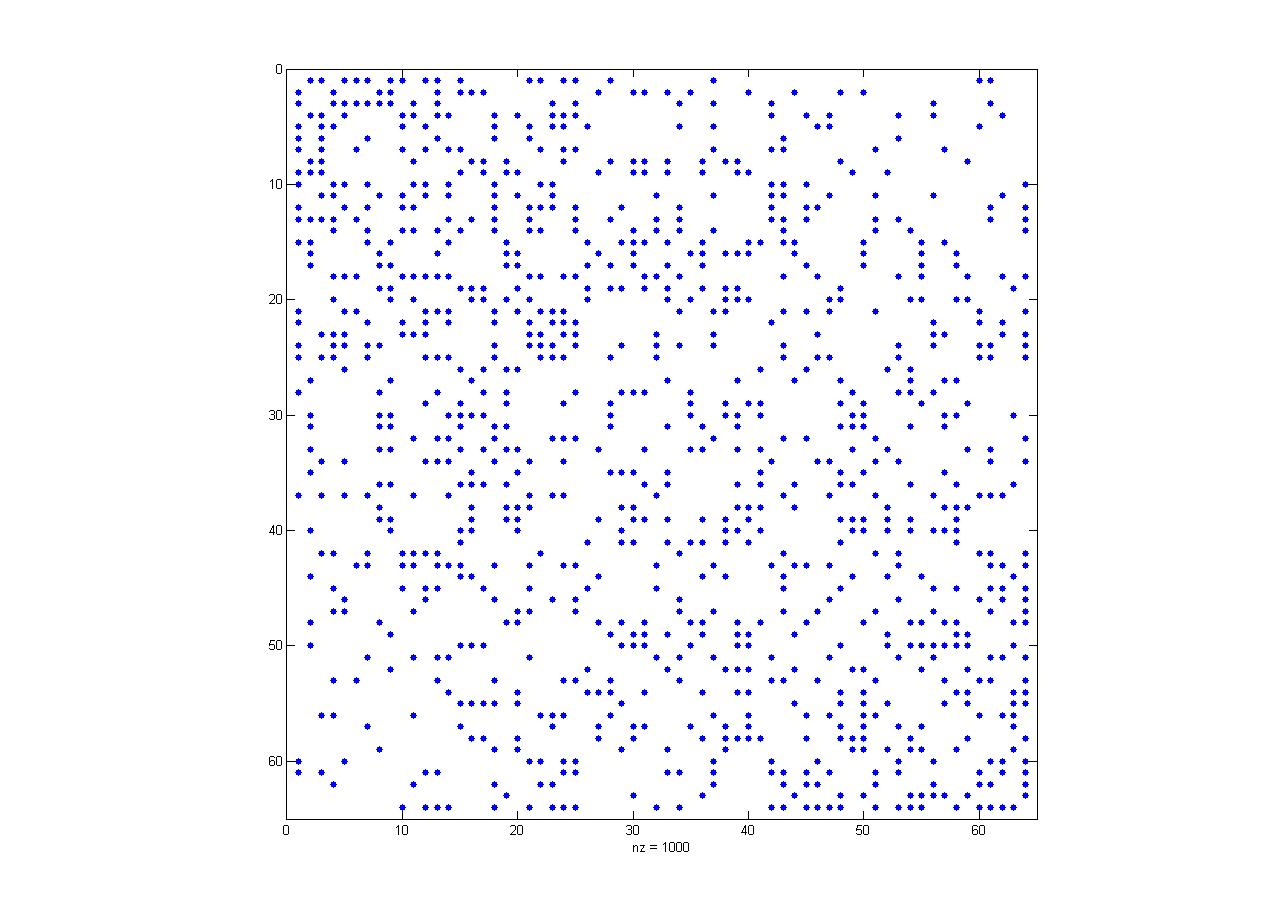
\includegraphics[width=5.0cm,height=5.0cm]{images/RandomGraph_WithCut_adjacencyMatrix_64Nodes.jpg}               &
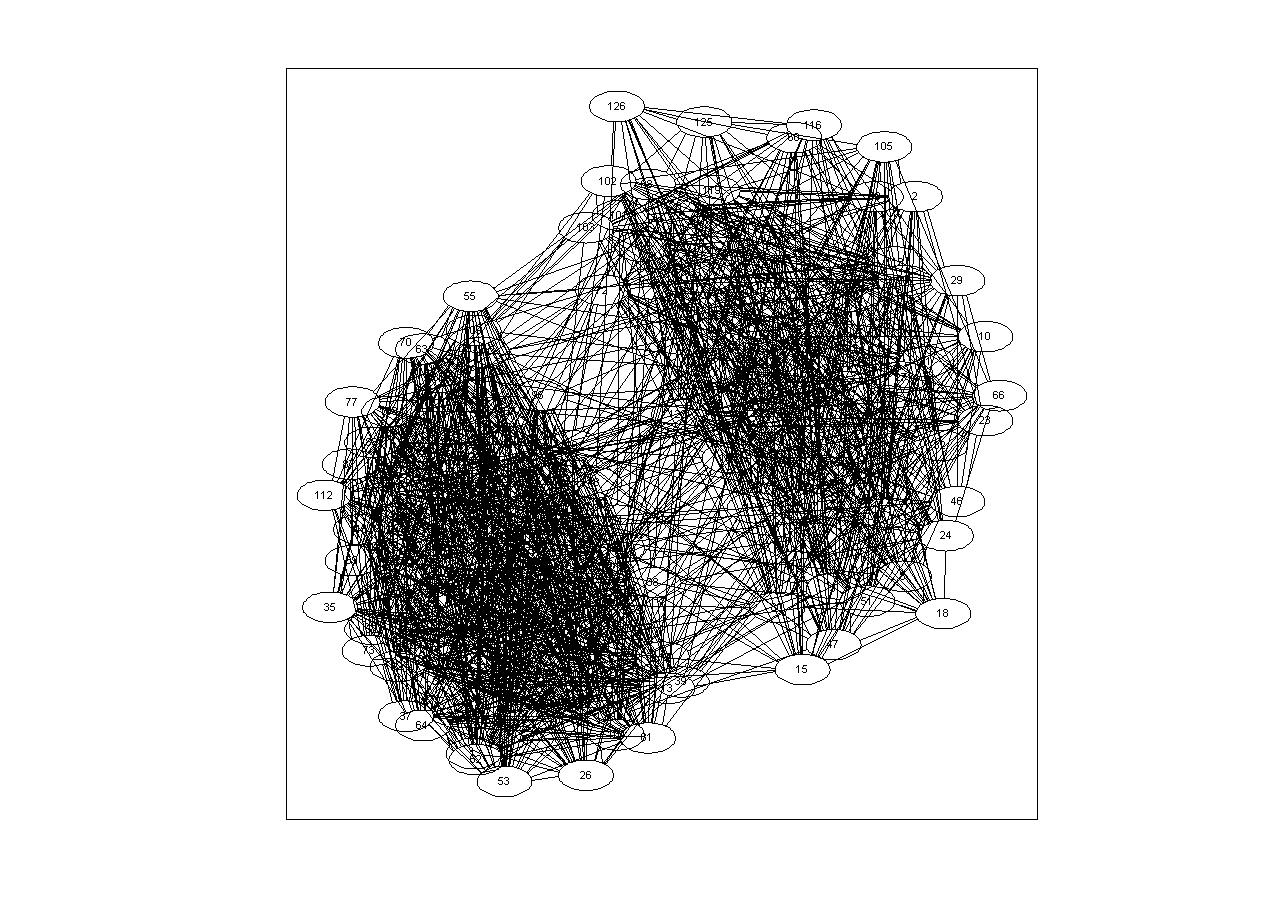
\includegraphics[width=5.0cm,height=5.0cm]{images/RandomGraph_WithCut_jpg.jpg}                                    &
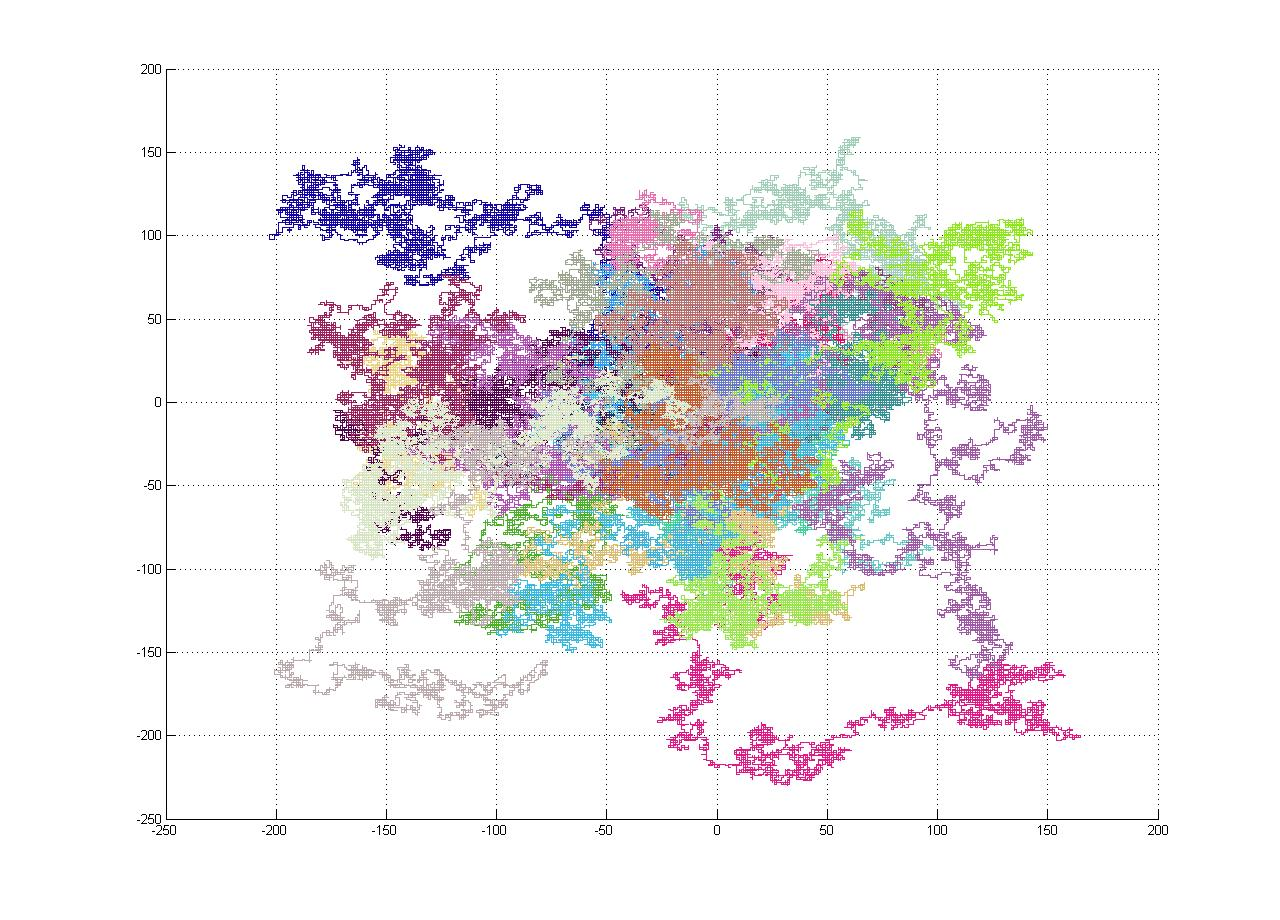
\includegraphics[width=5.0cm,height=5.0cm]{images/RandomWalk_30_Walkers_20000_steps.jpg}                           \\
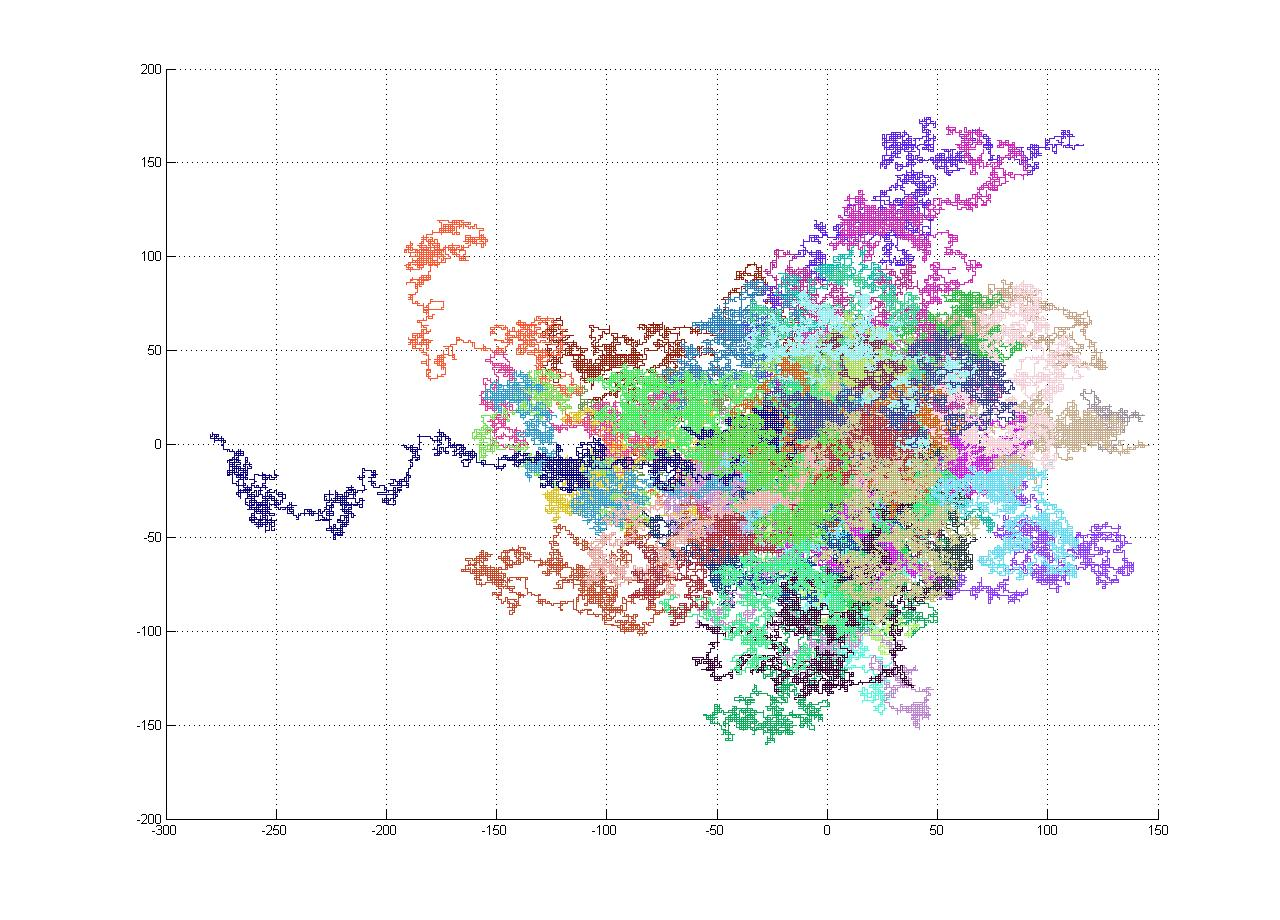
\includegraphics[width=5.0cm,height=5.0cm]{images/RandomWalk_50_Walkers.jpg}                           &
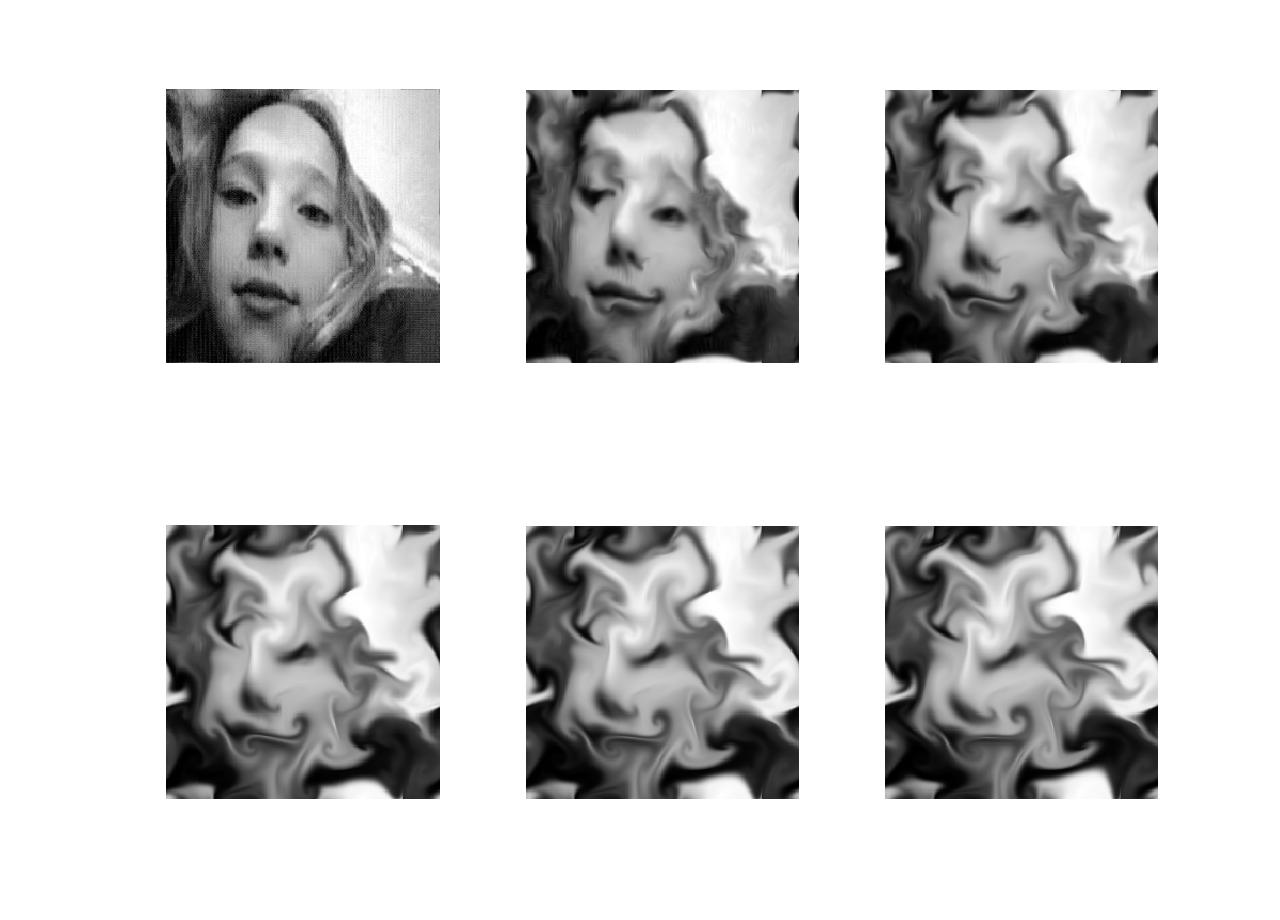
\includegraphics[width=5.0cm,height=5.0cm]{images/Raymond_AdvectiveNavierStokesdiffusion.jpg}           &
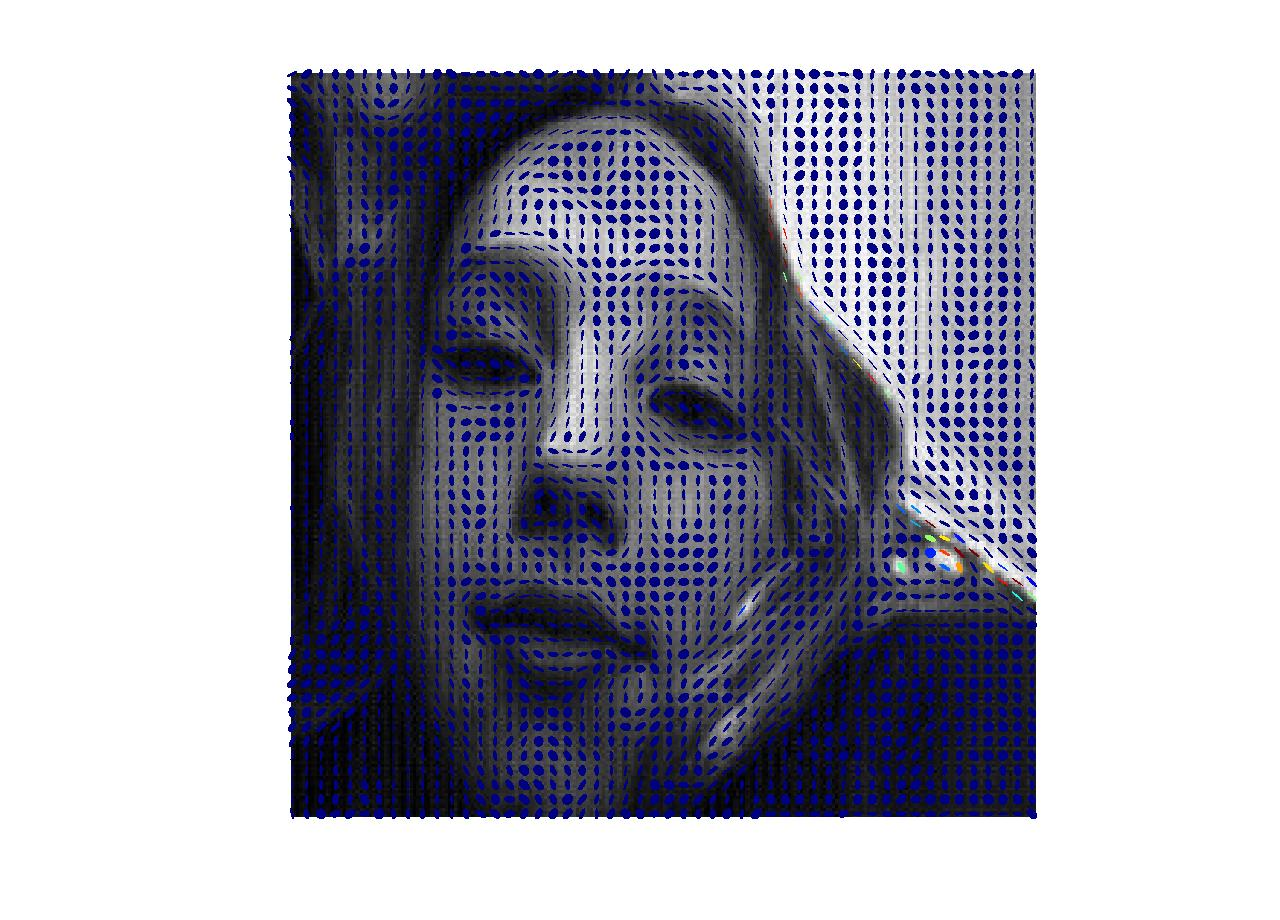
\includegraphics[width=5.0cm,height=5.0cm]{images/Raymond_TensorField.jpg}
\end{tabular}

\begin{tabular}{ |c|c|c| }
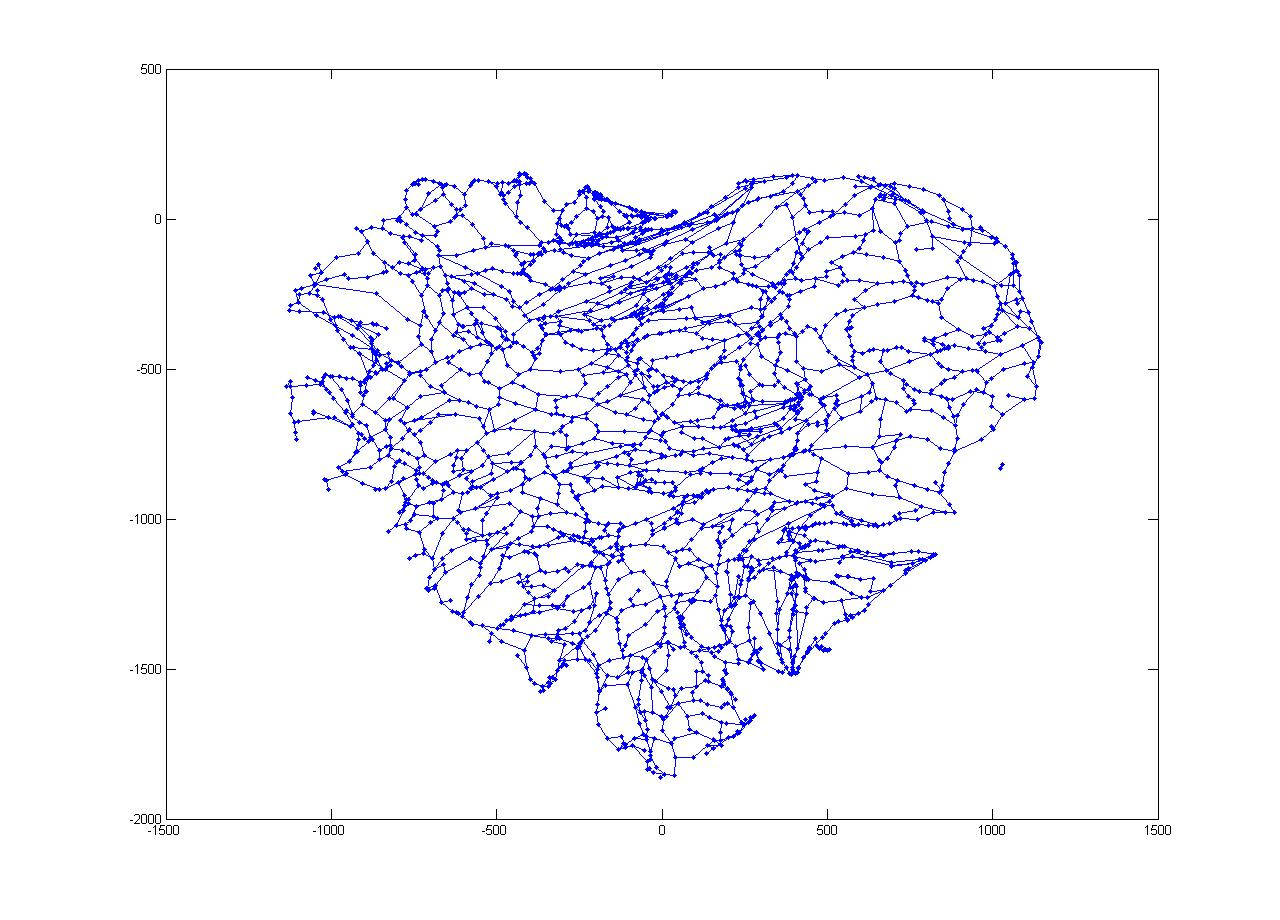
\includegraphics[width=5.0cm,height=5.0cm]{images/RoadMap.jpg}                                             &
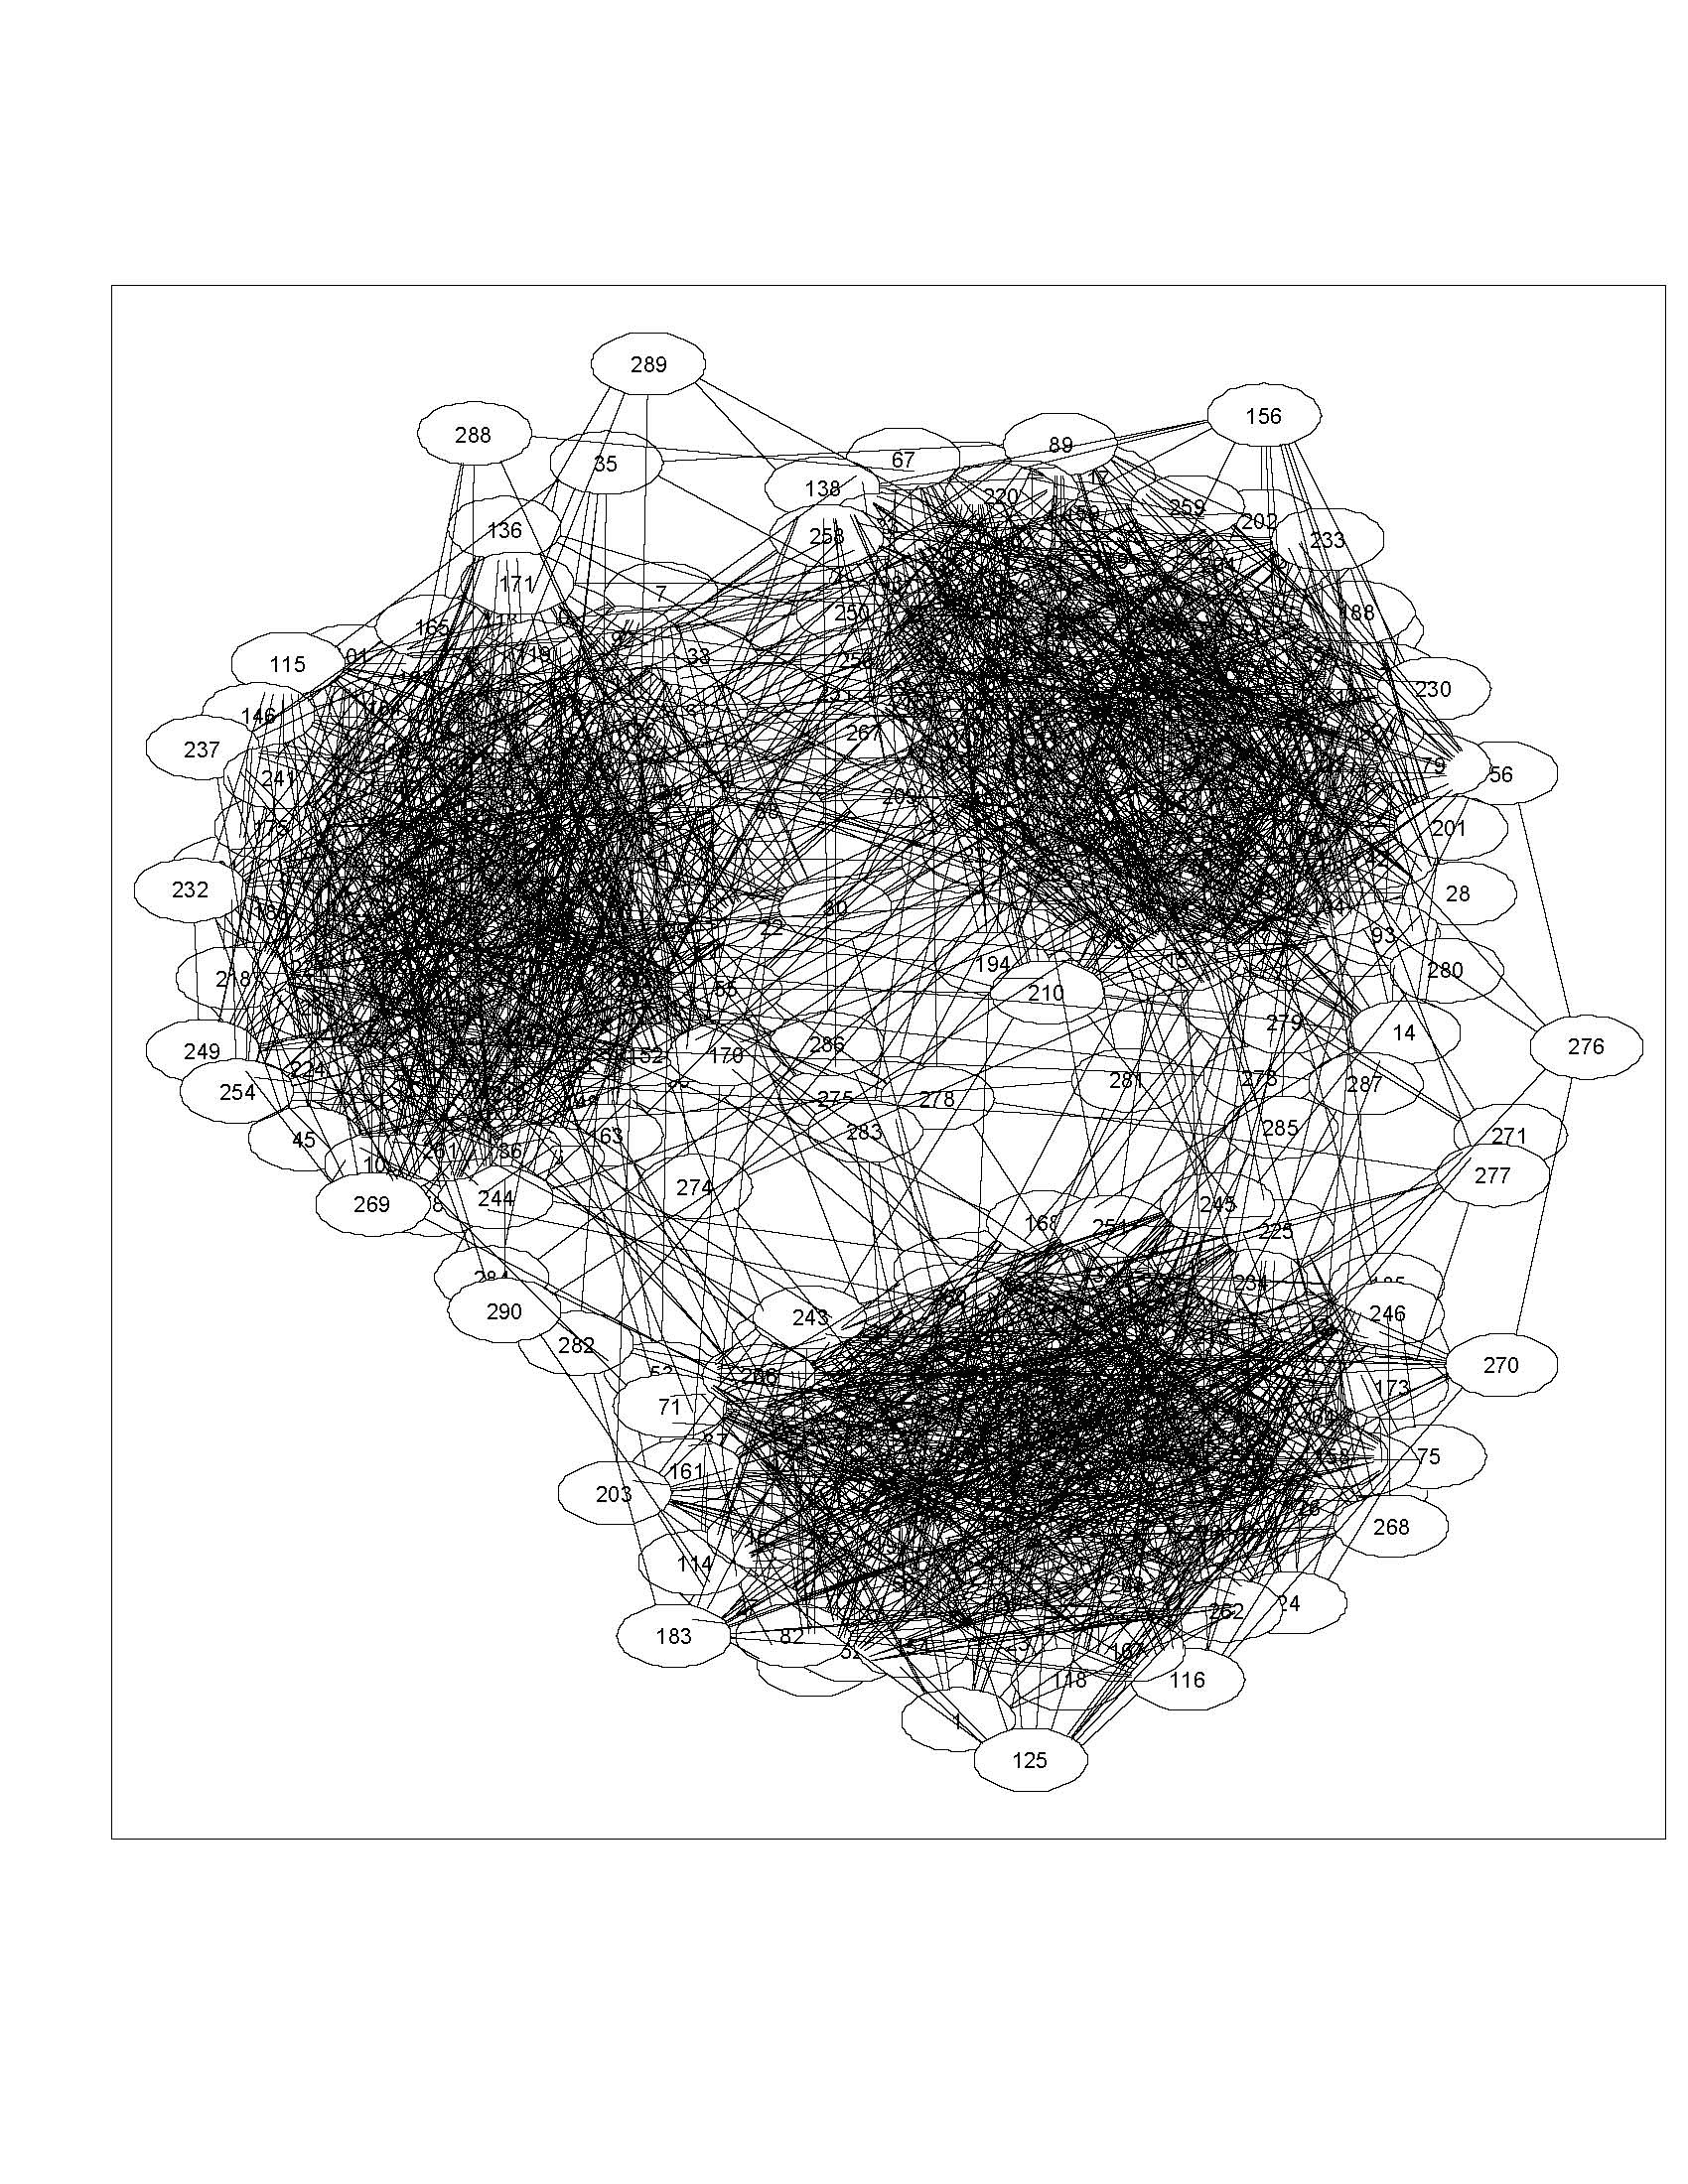
\includegraphics[width=5.0cm,height=5.0cm]{images/ScaleFreeClusterGraph.jpg}                                &
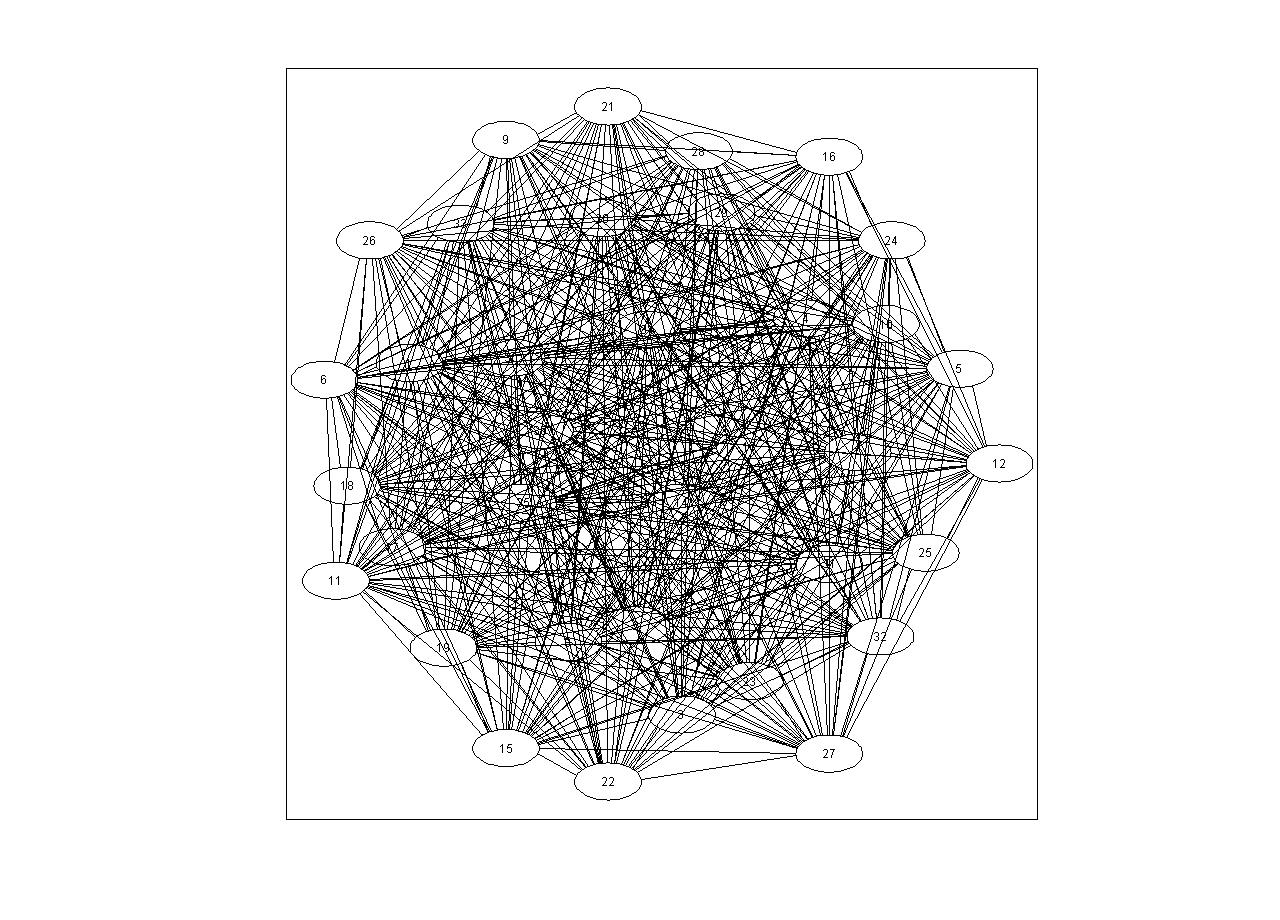
\includegraphics[width=5.0cm,height=5.0cm]{images/WellConnectedWithRedBlackOrder_Bipatate.jpg}               \\
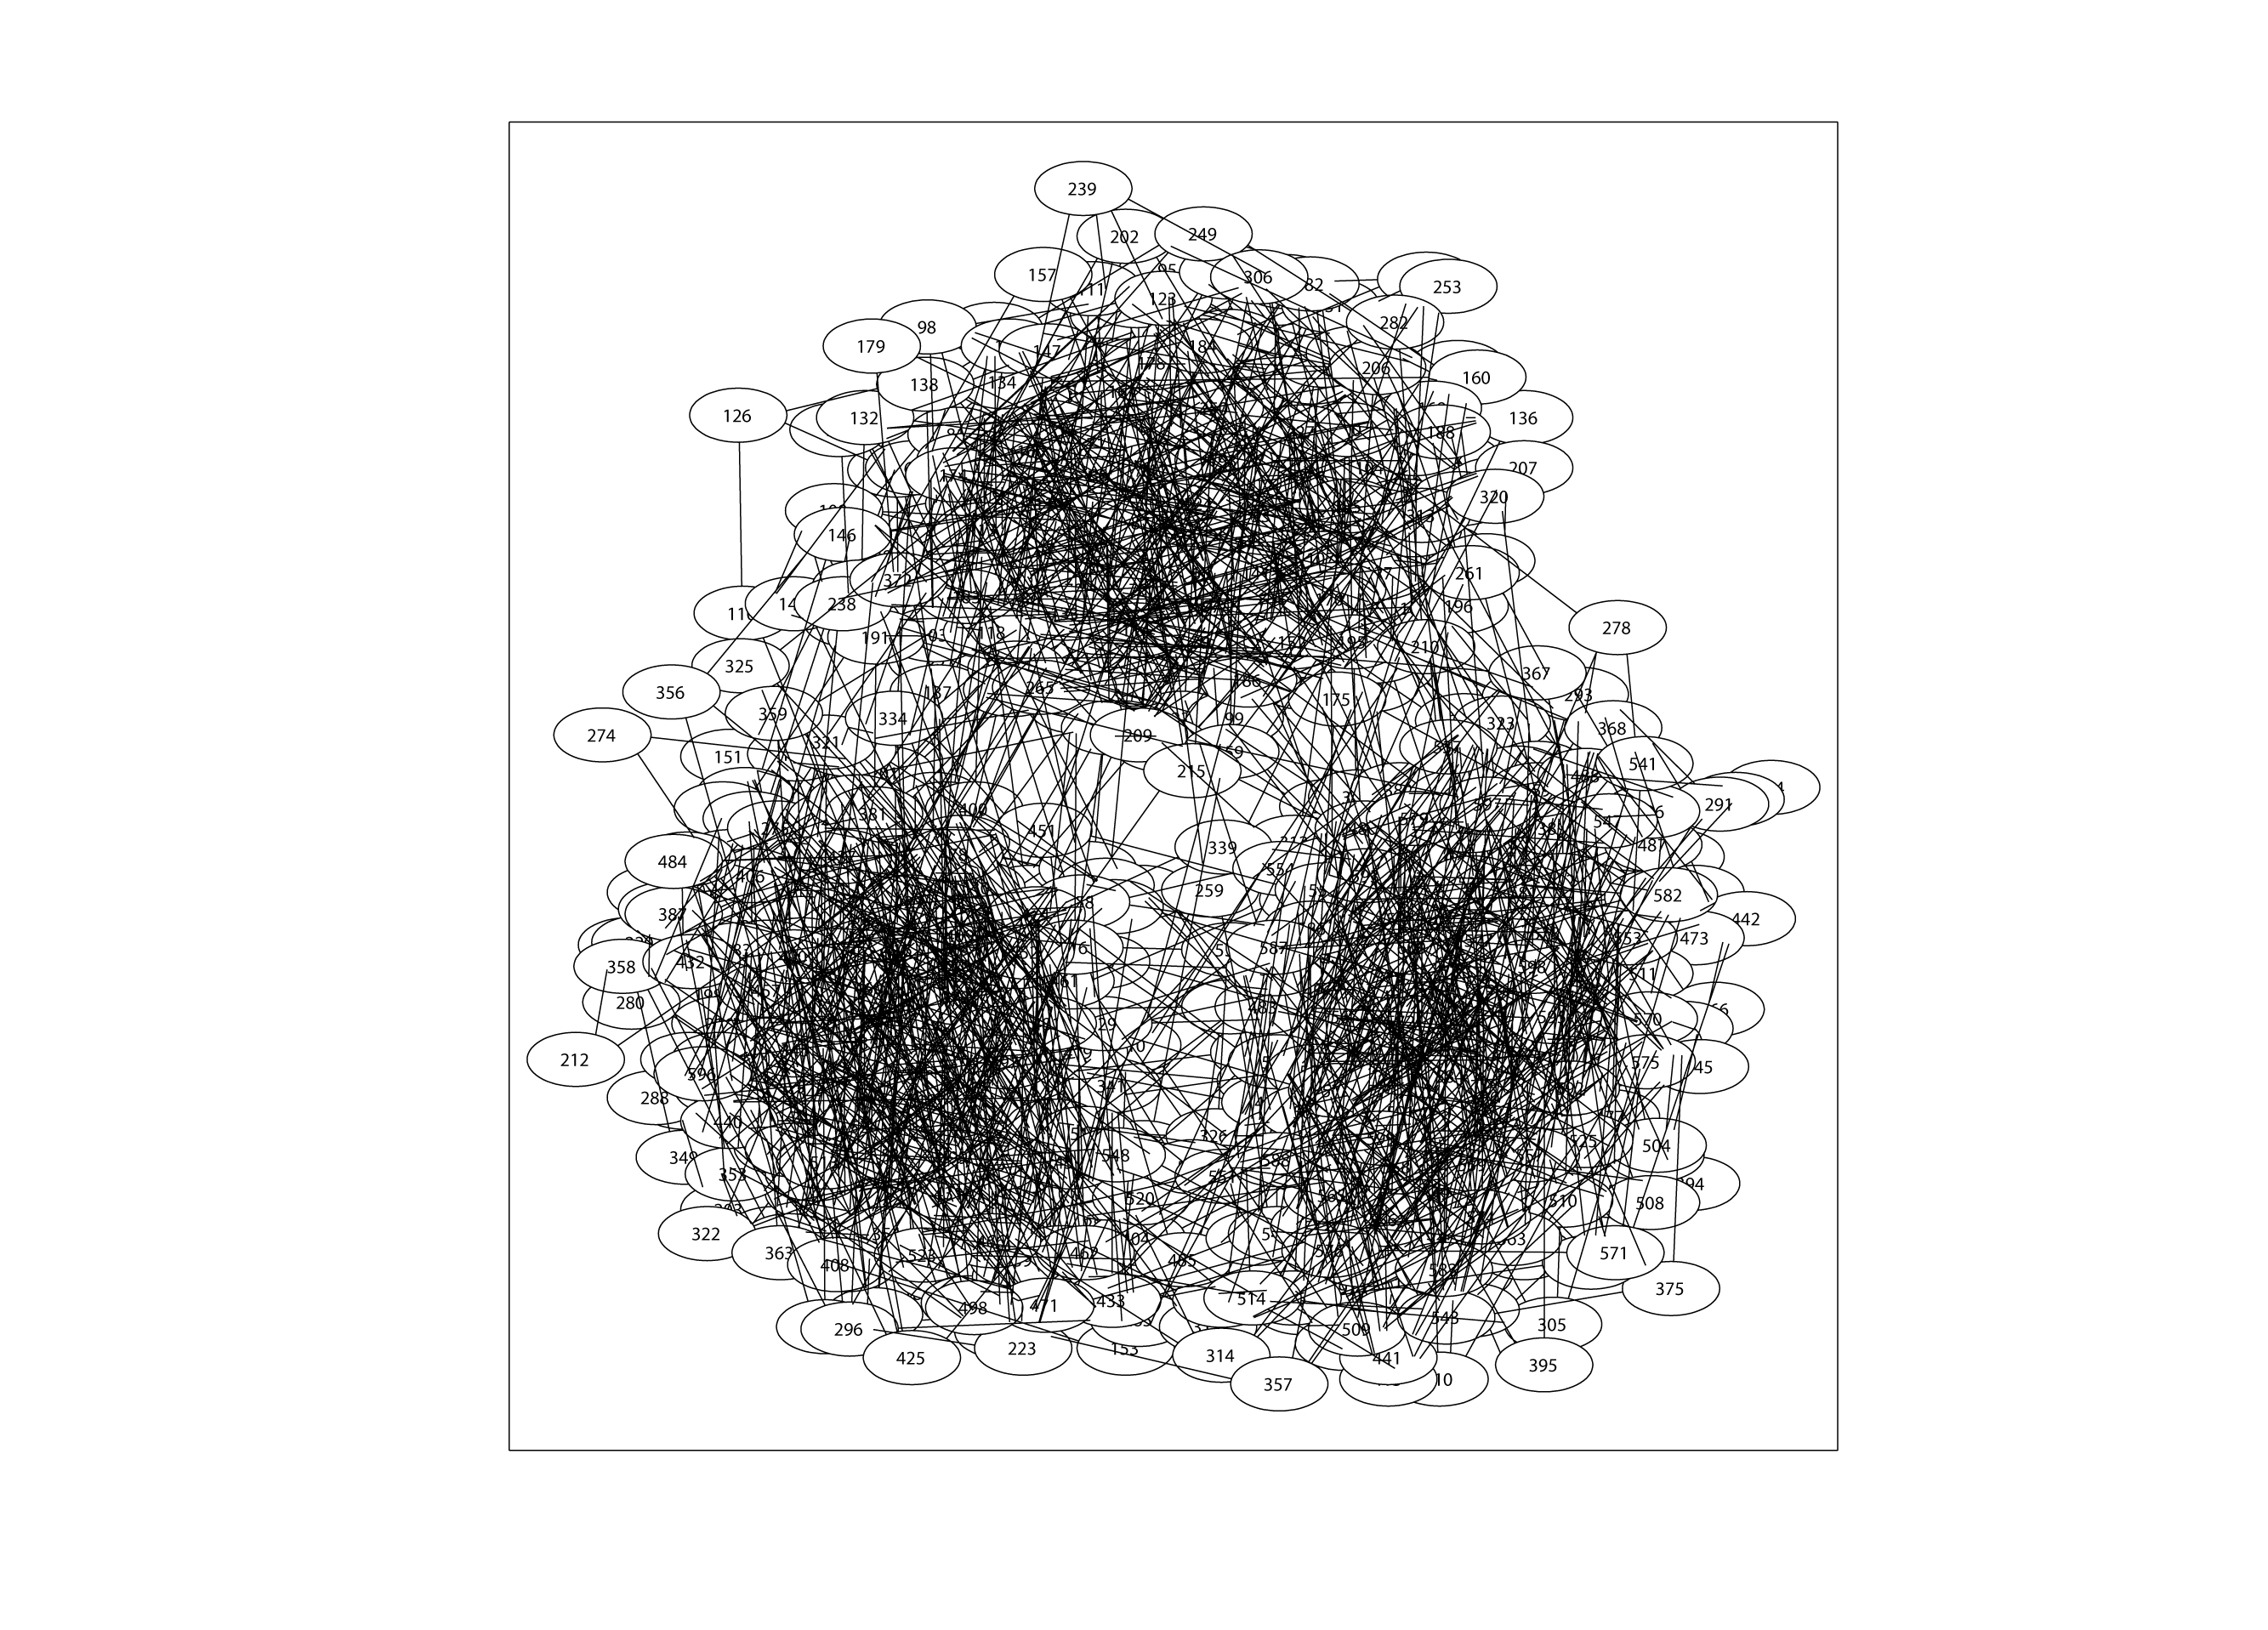
\includegraphics[width=5.0cm,height=5.0cm]{images/WellConnectedWithThreeClusters.jpg}                          &
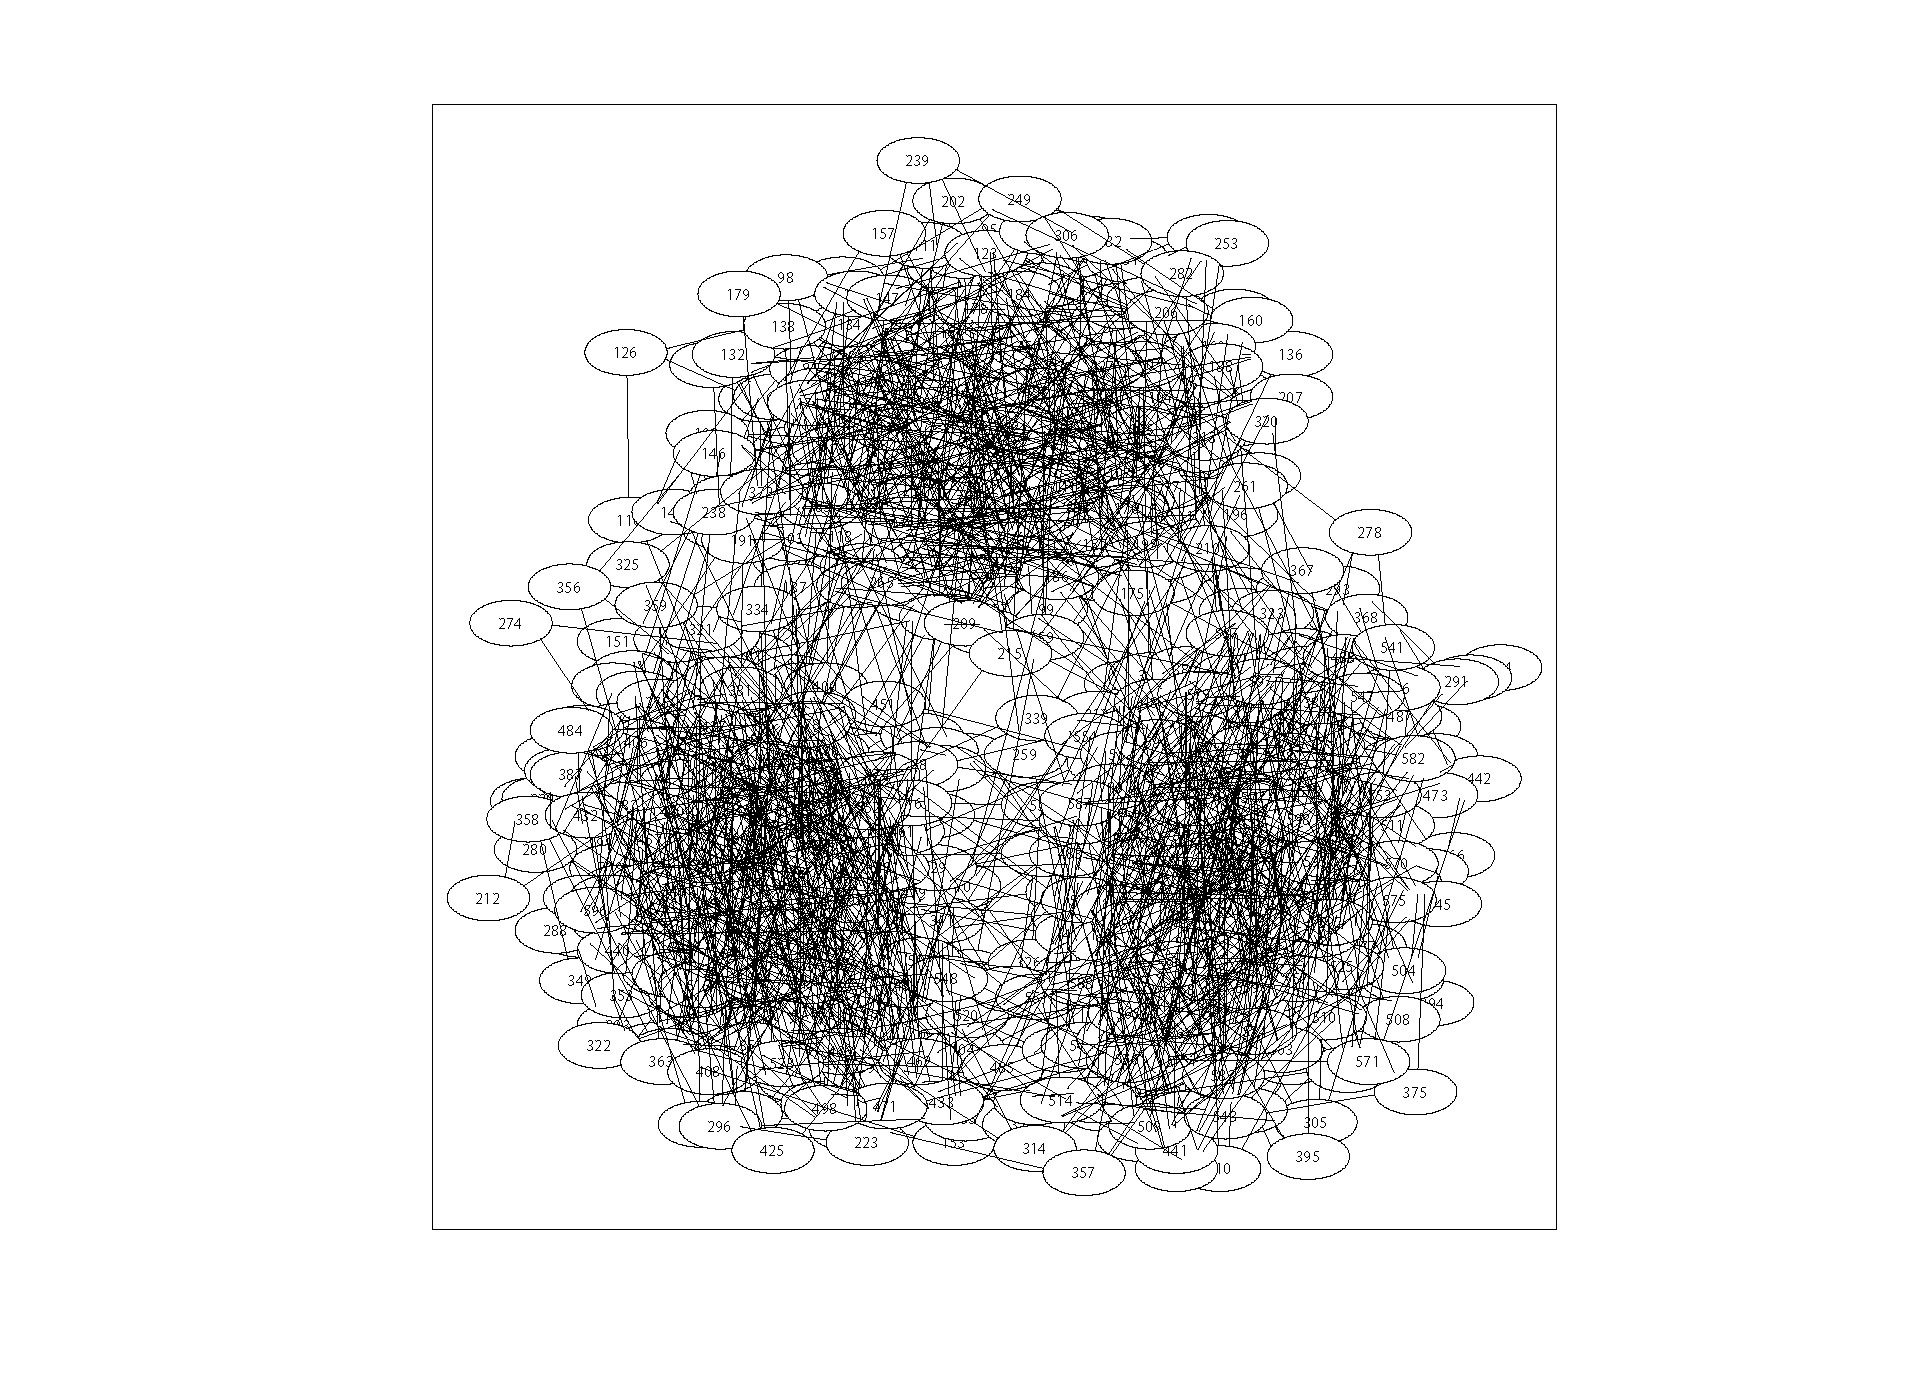
\includegraphics[width=5.0cm,height=5.0cm]{images/WellConnectedWithThreeClusters2.jpg}                          &
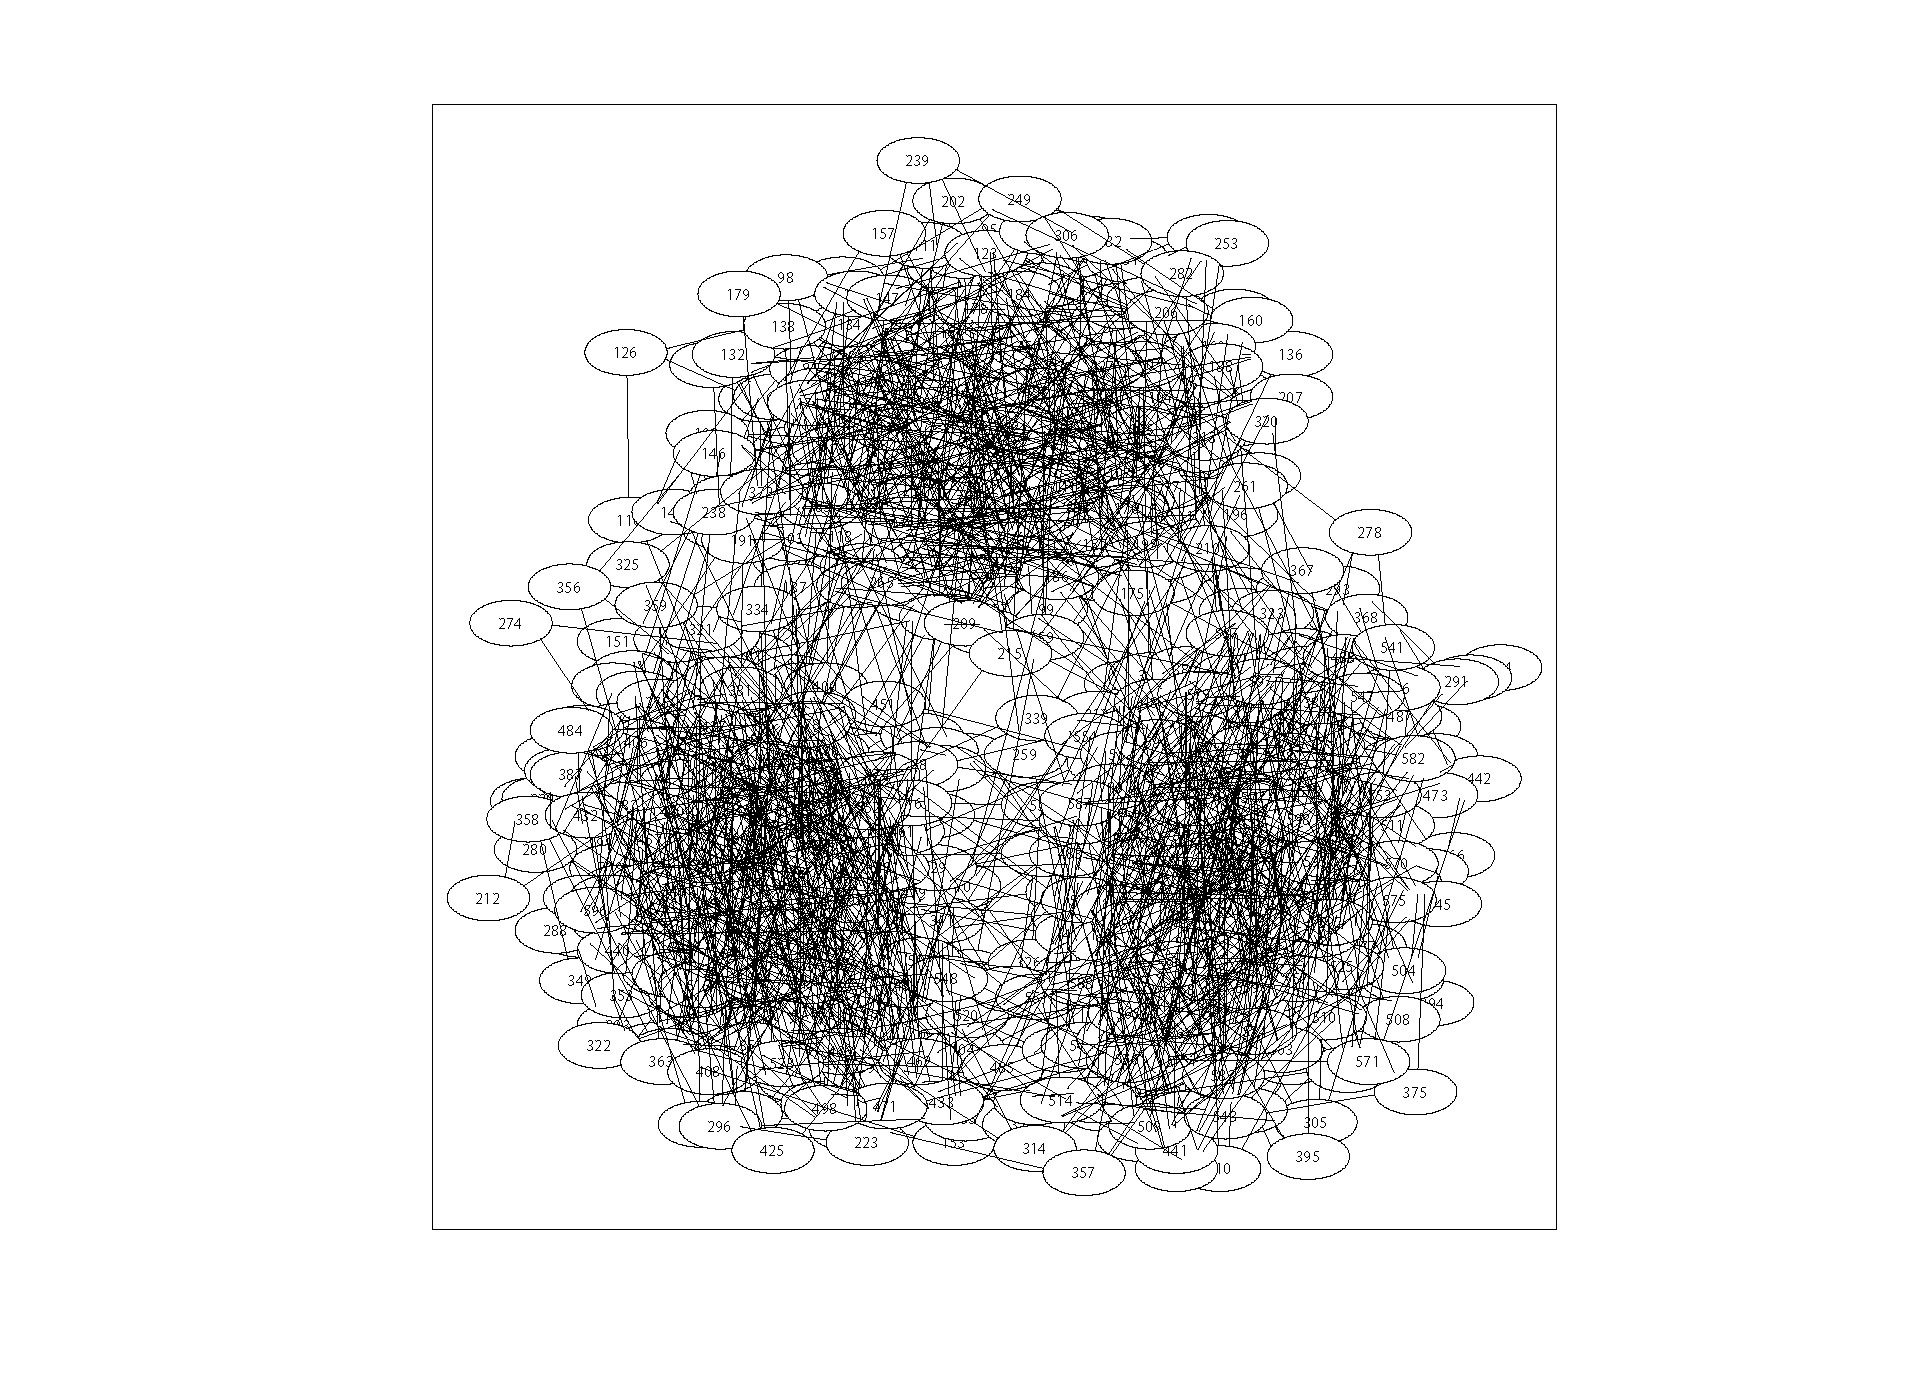
\includegraphics[width=5.0cm,height=5.0cm]{images/WellConnectedWithThreeClusters3.jpg}
\end{tabular}


\begin{tabular}{ |c|c|c| }
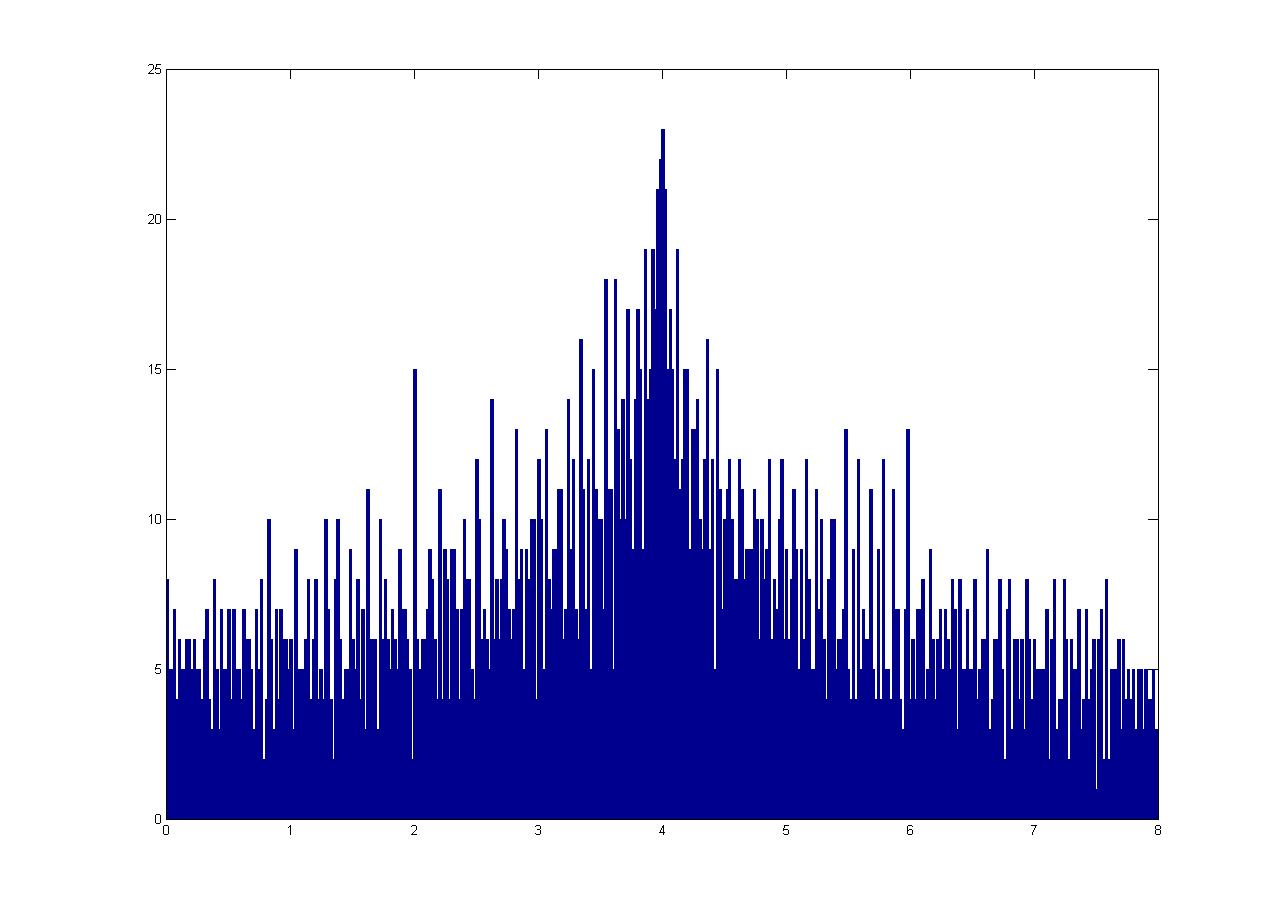
\includegraphics[width=5.0cm,height=5.0cm]{images/60_50_grid_graph_spectra.jpg} &
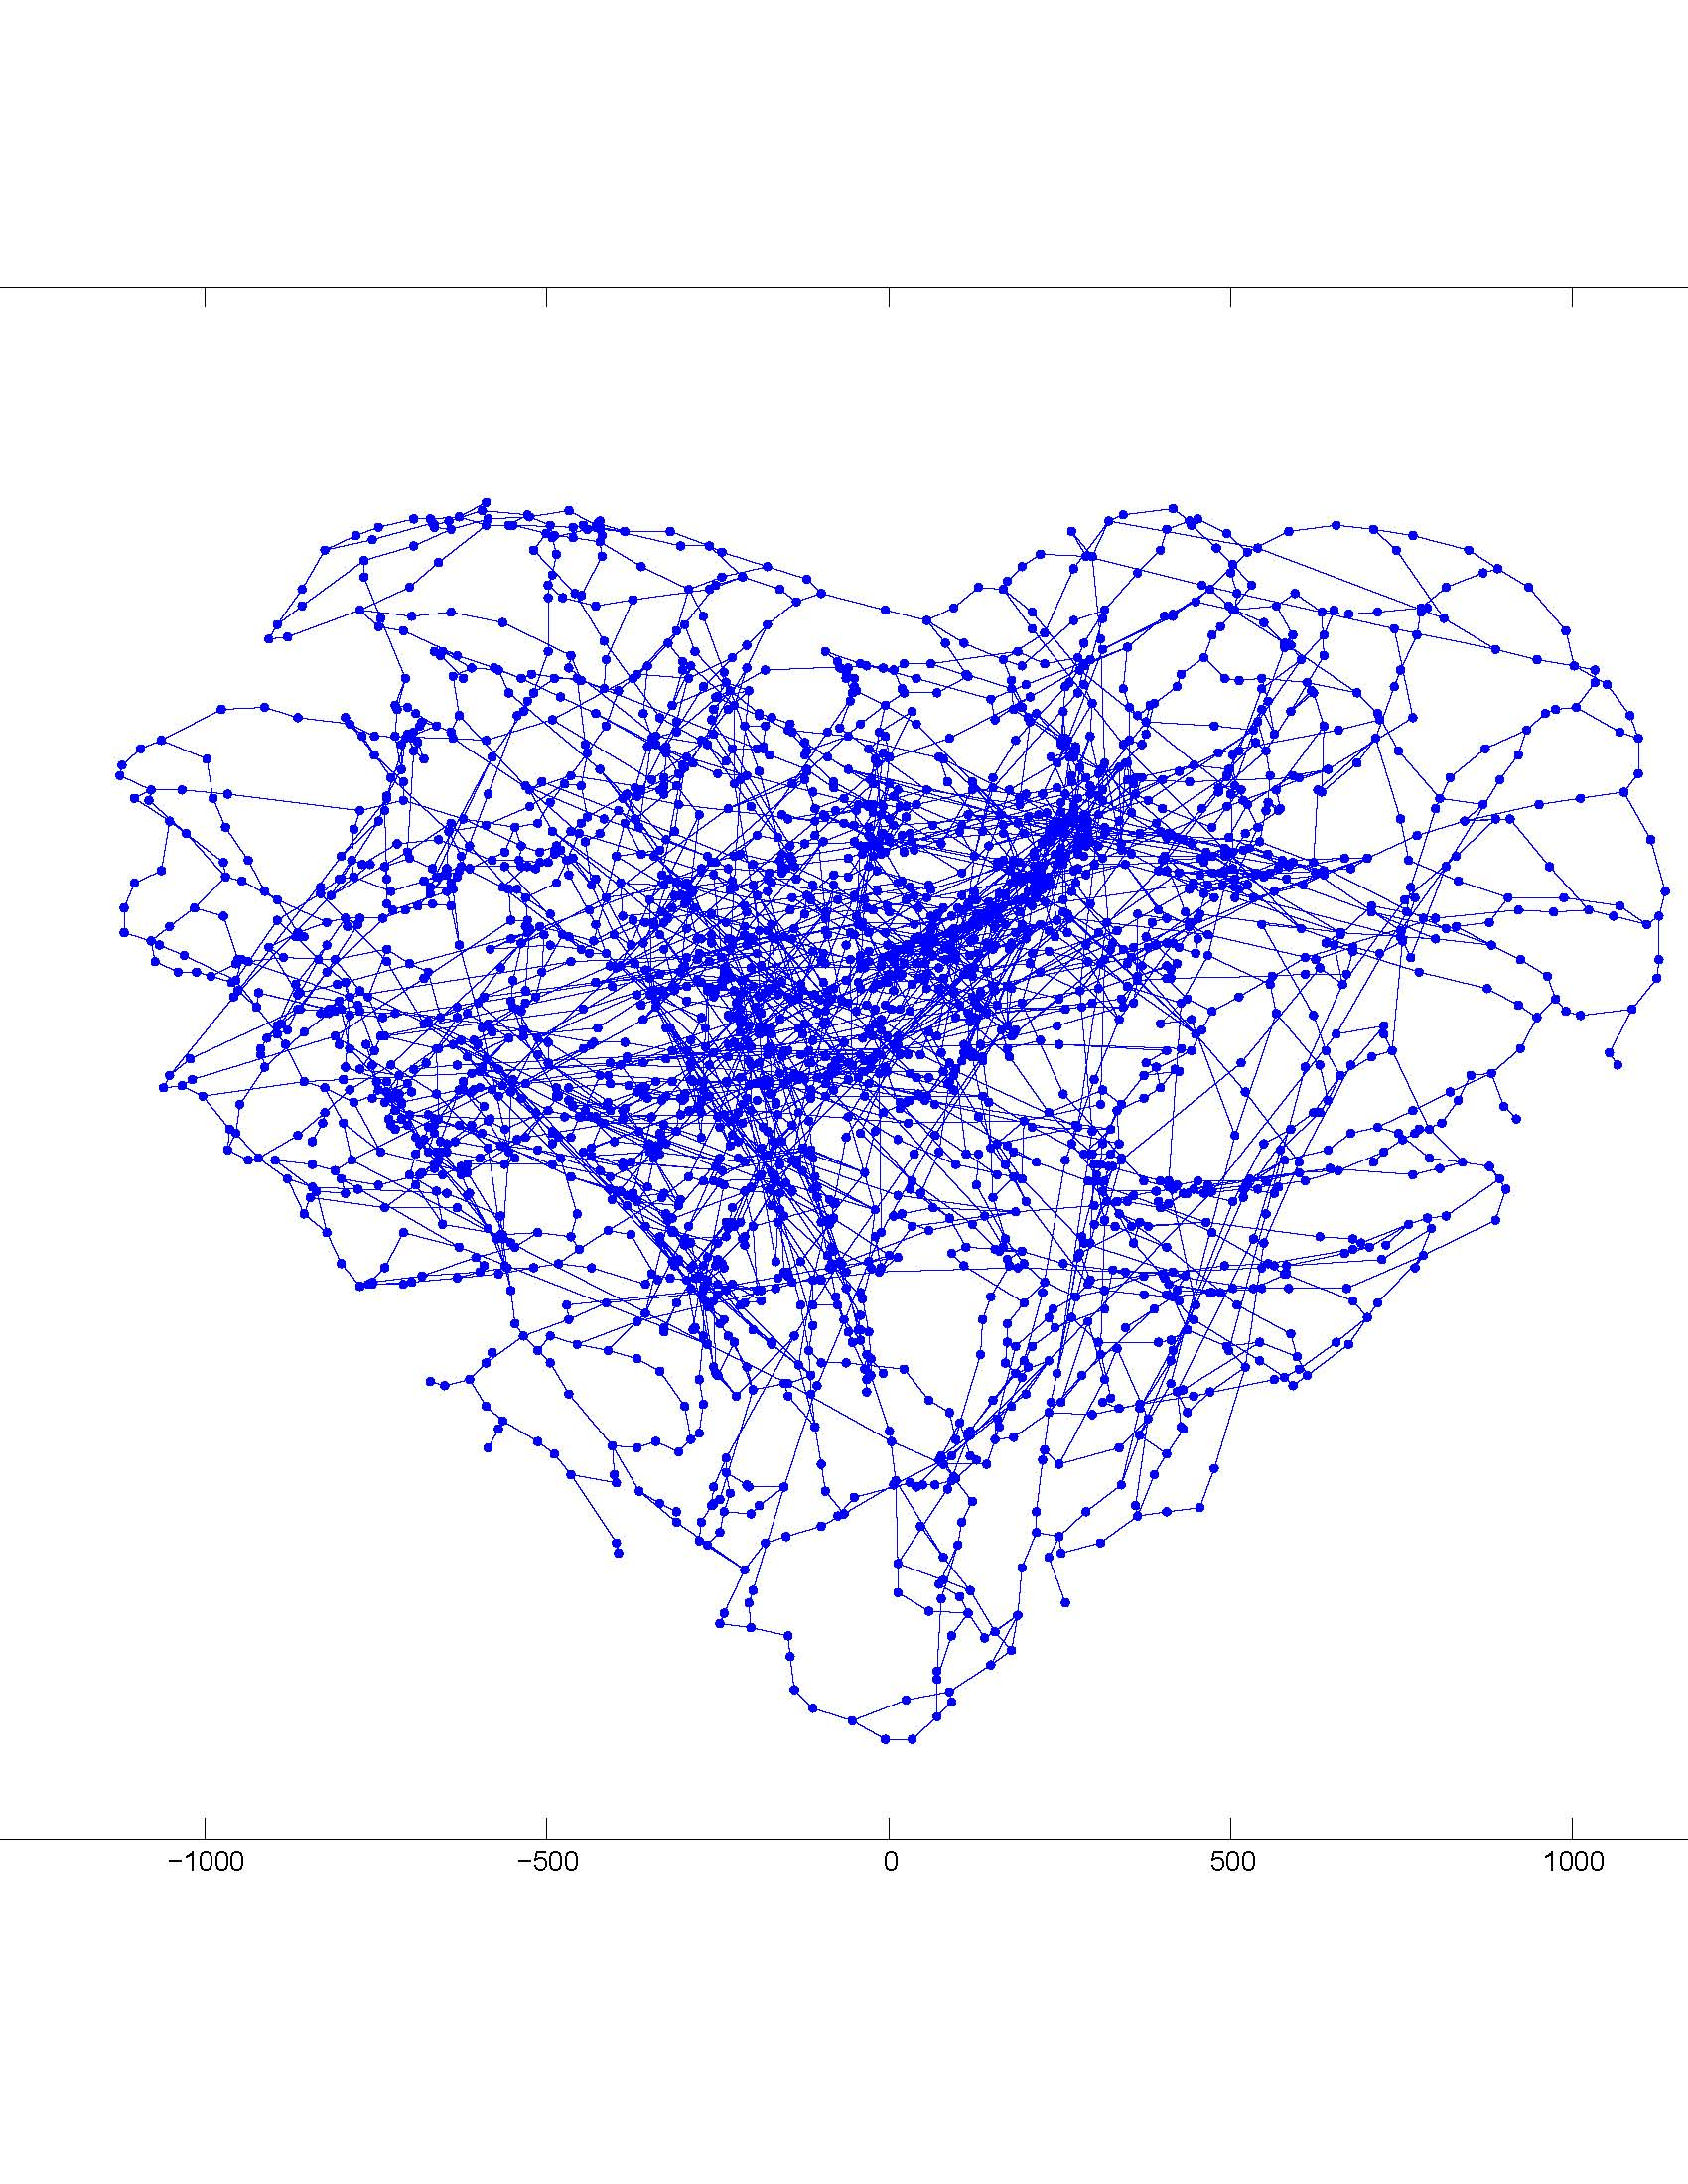
\includegraphics[width=5.0cm,height=5.0cm]{images/RoadNetwork_Scalefree_100v_c2.jpg} \\
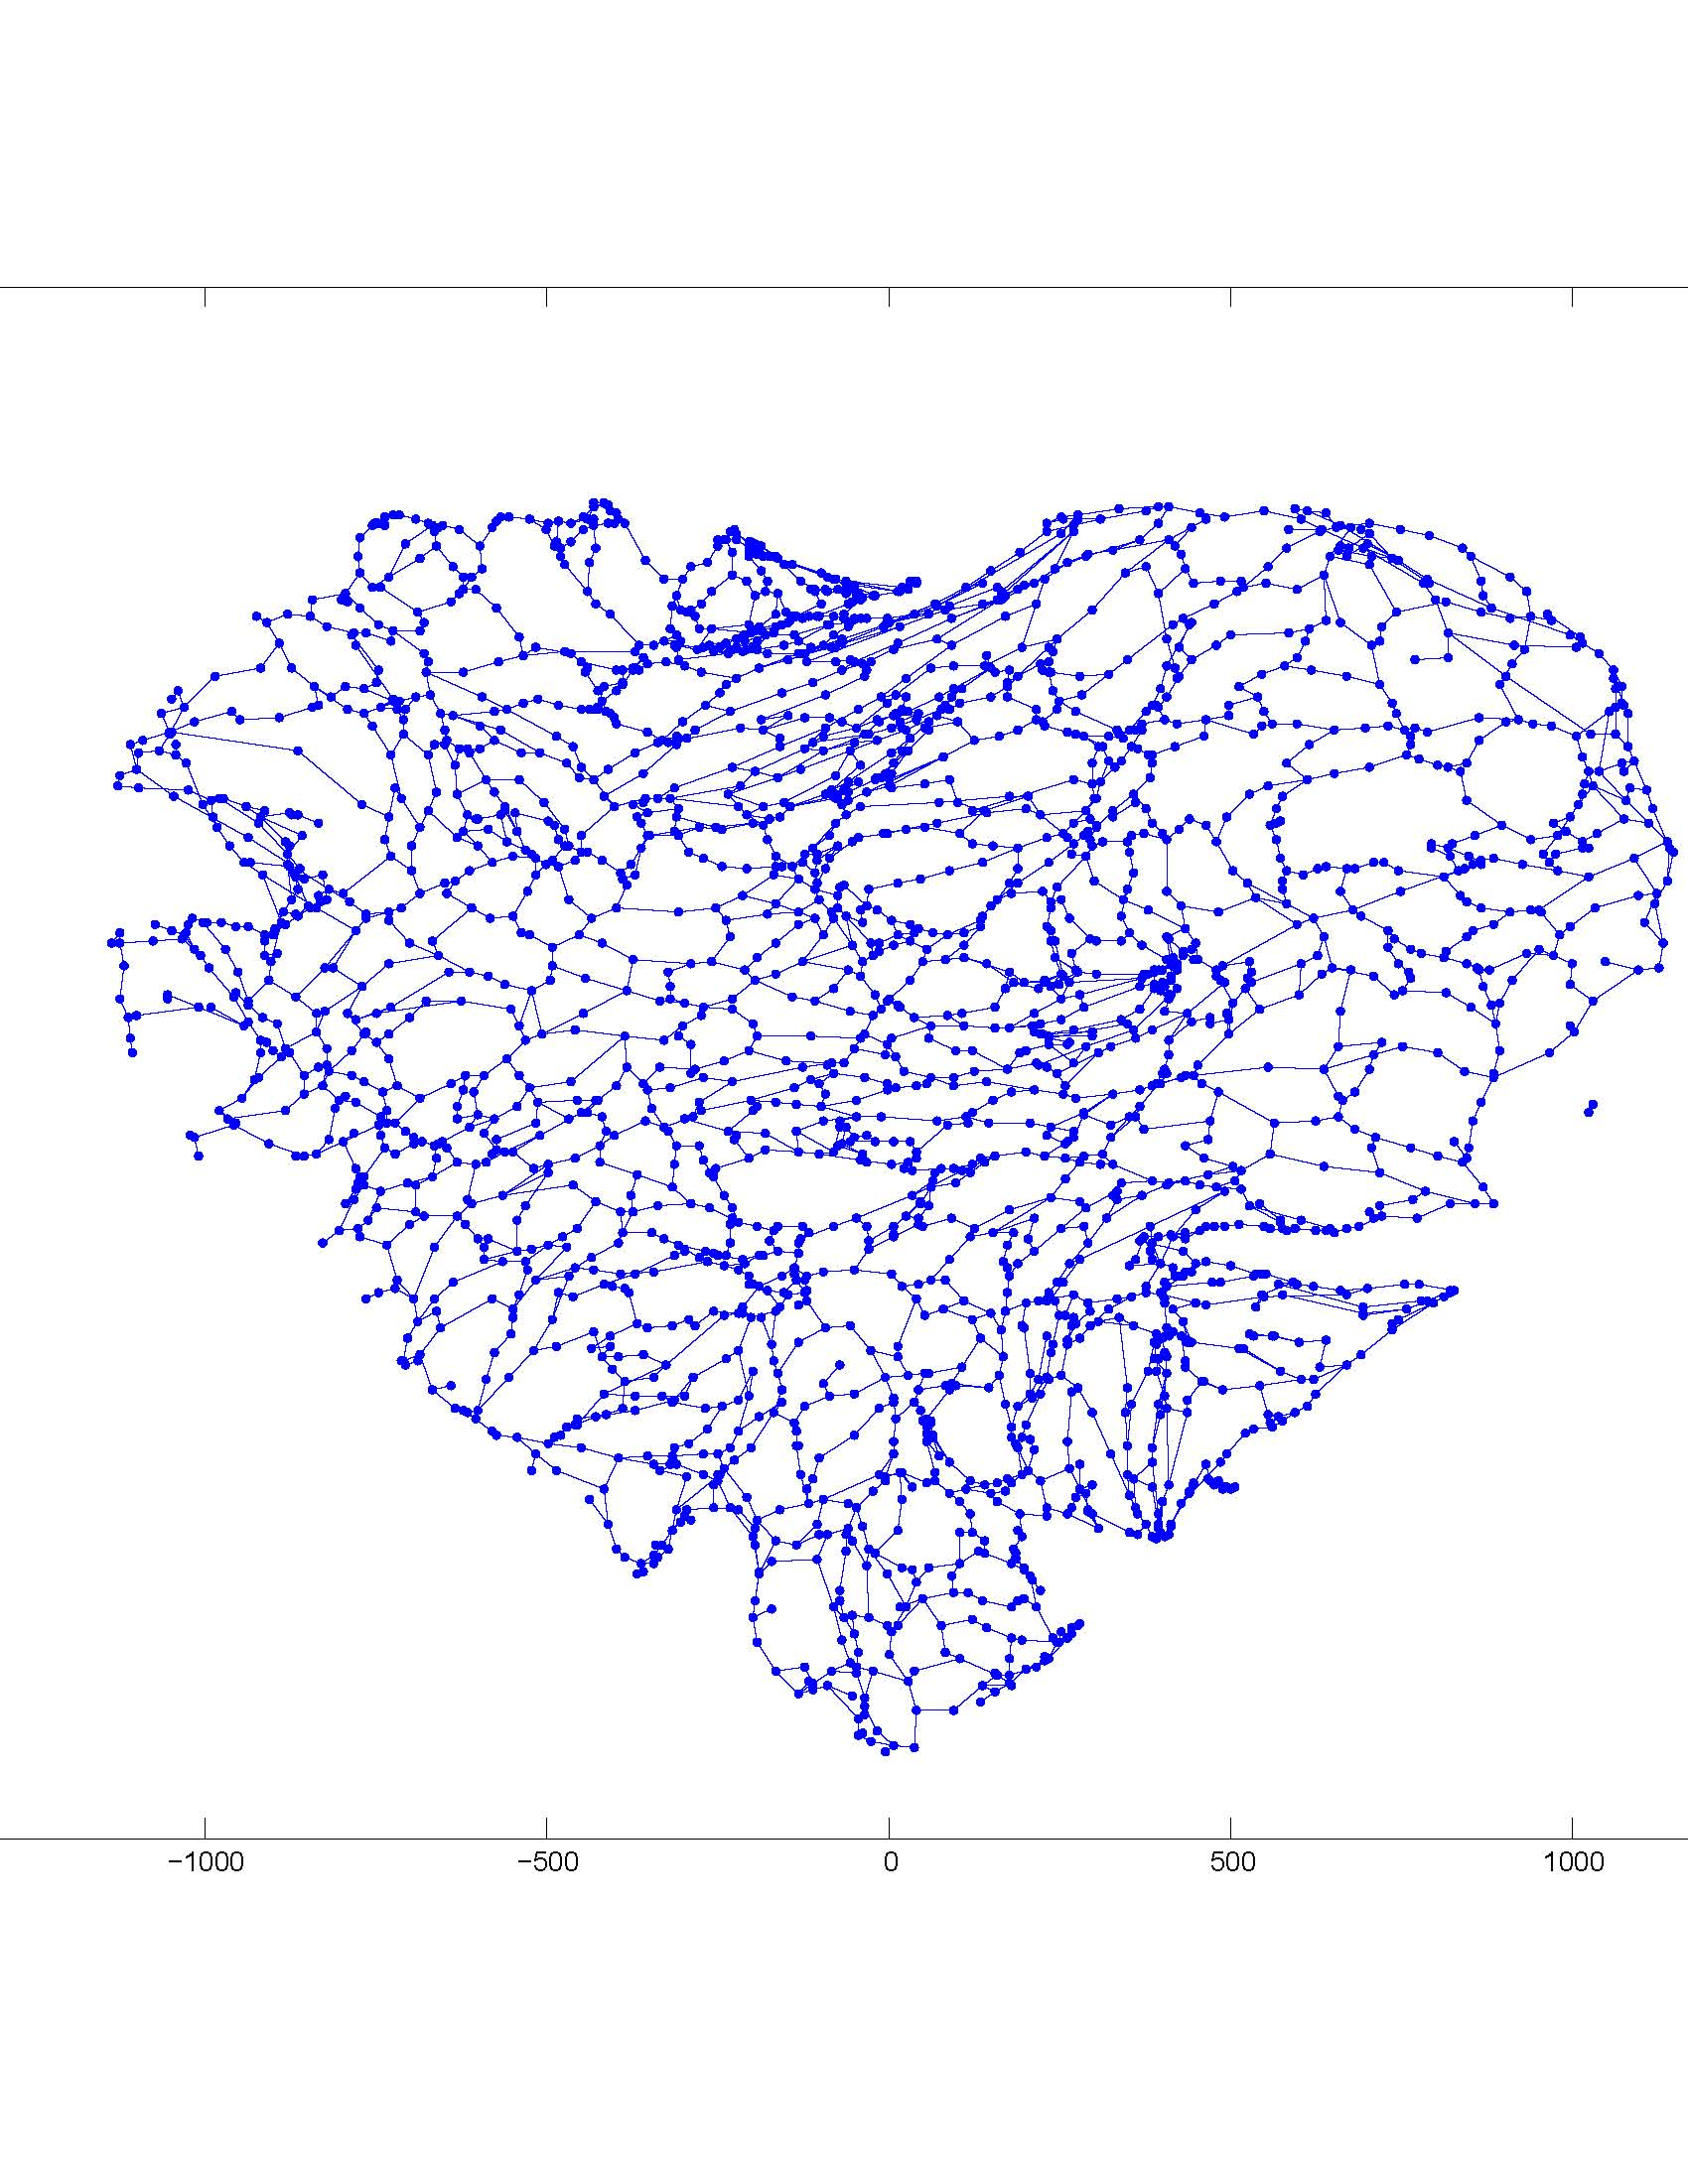
\includegraphics[width=5.0cm,height=5.0cm]{images/GursoyAtunScaleFreeAB.jpg} &
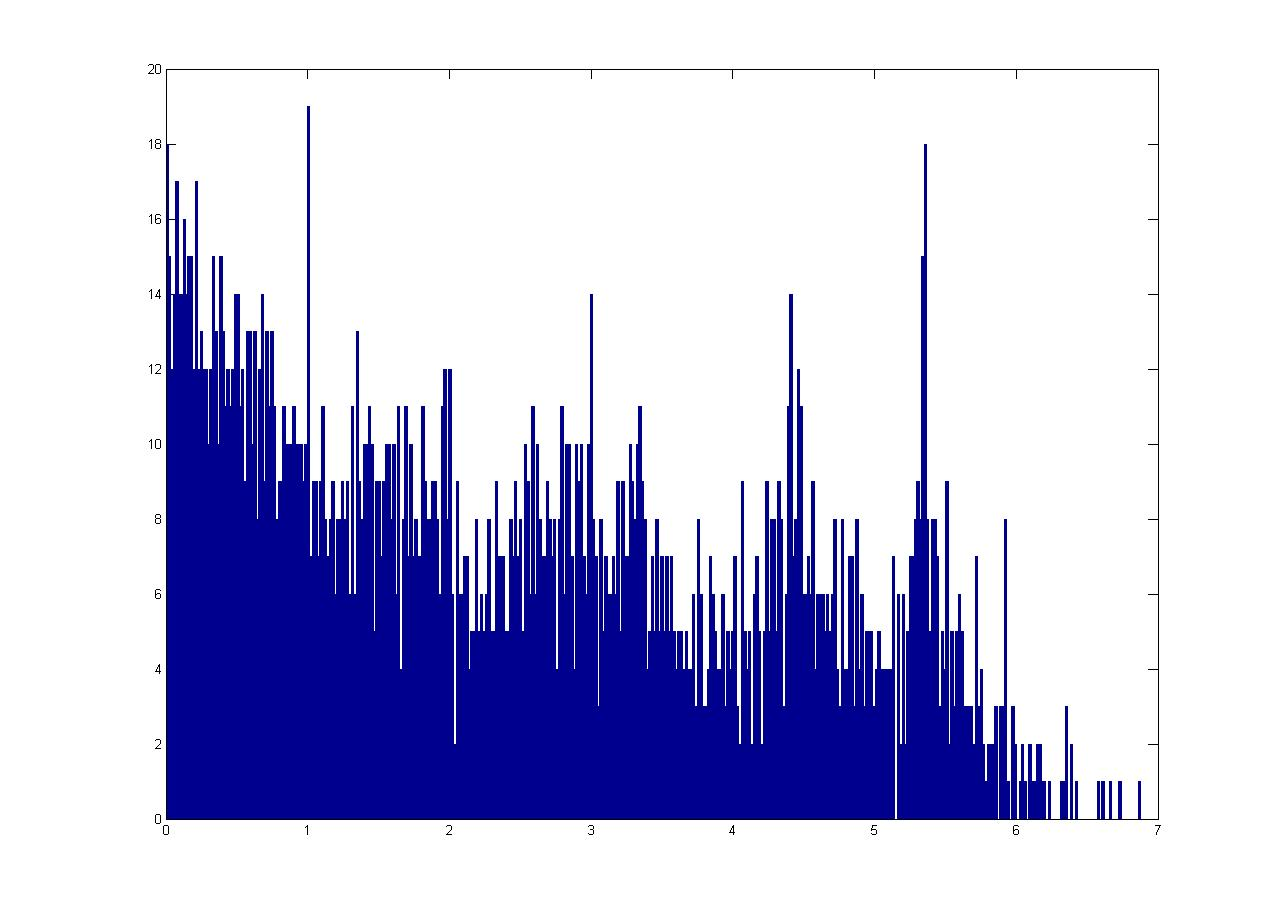
\includegraphics[width=5.0cm,height=5.0cm]{images/spectra_minnesotaRoad_network.jpg}
\end{tabular}




\subsection{Cell Segmentation \& Automated Pathology}
%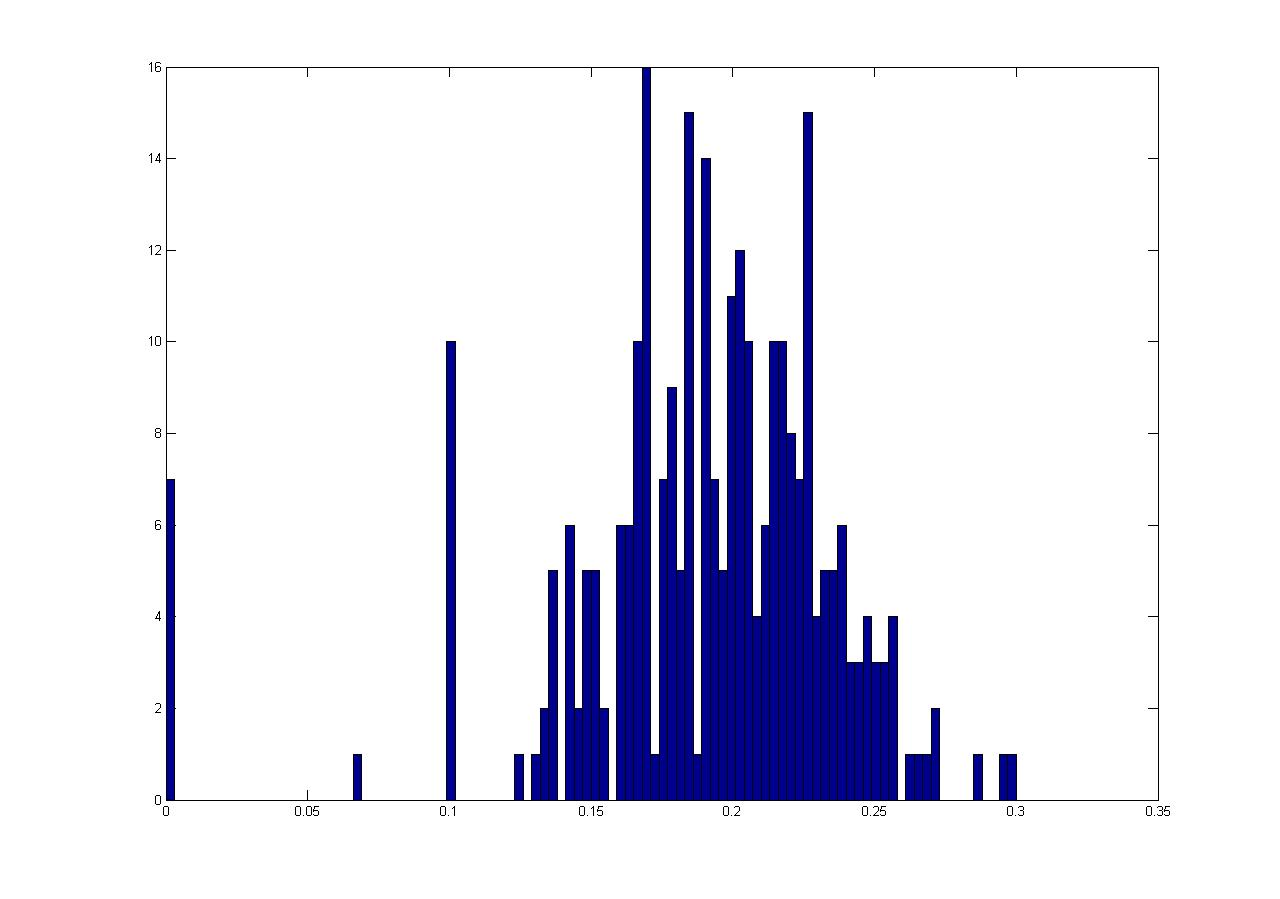
\includegraphics[width=5.0cm,height=5.0cm]{images/GraphTheory/ClusterCoeff_Hist_ScaleFree_with20ExtraNode_5maxE_mean_0_190053489673149.jpg}

\begin{tabular}{ |c|c|c| }
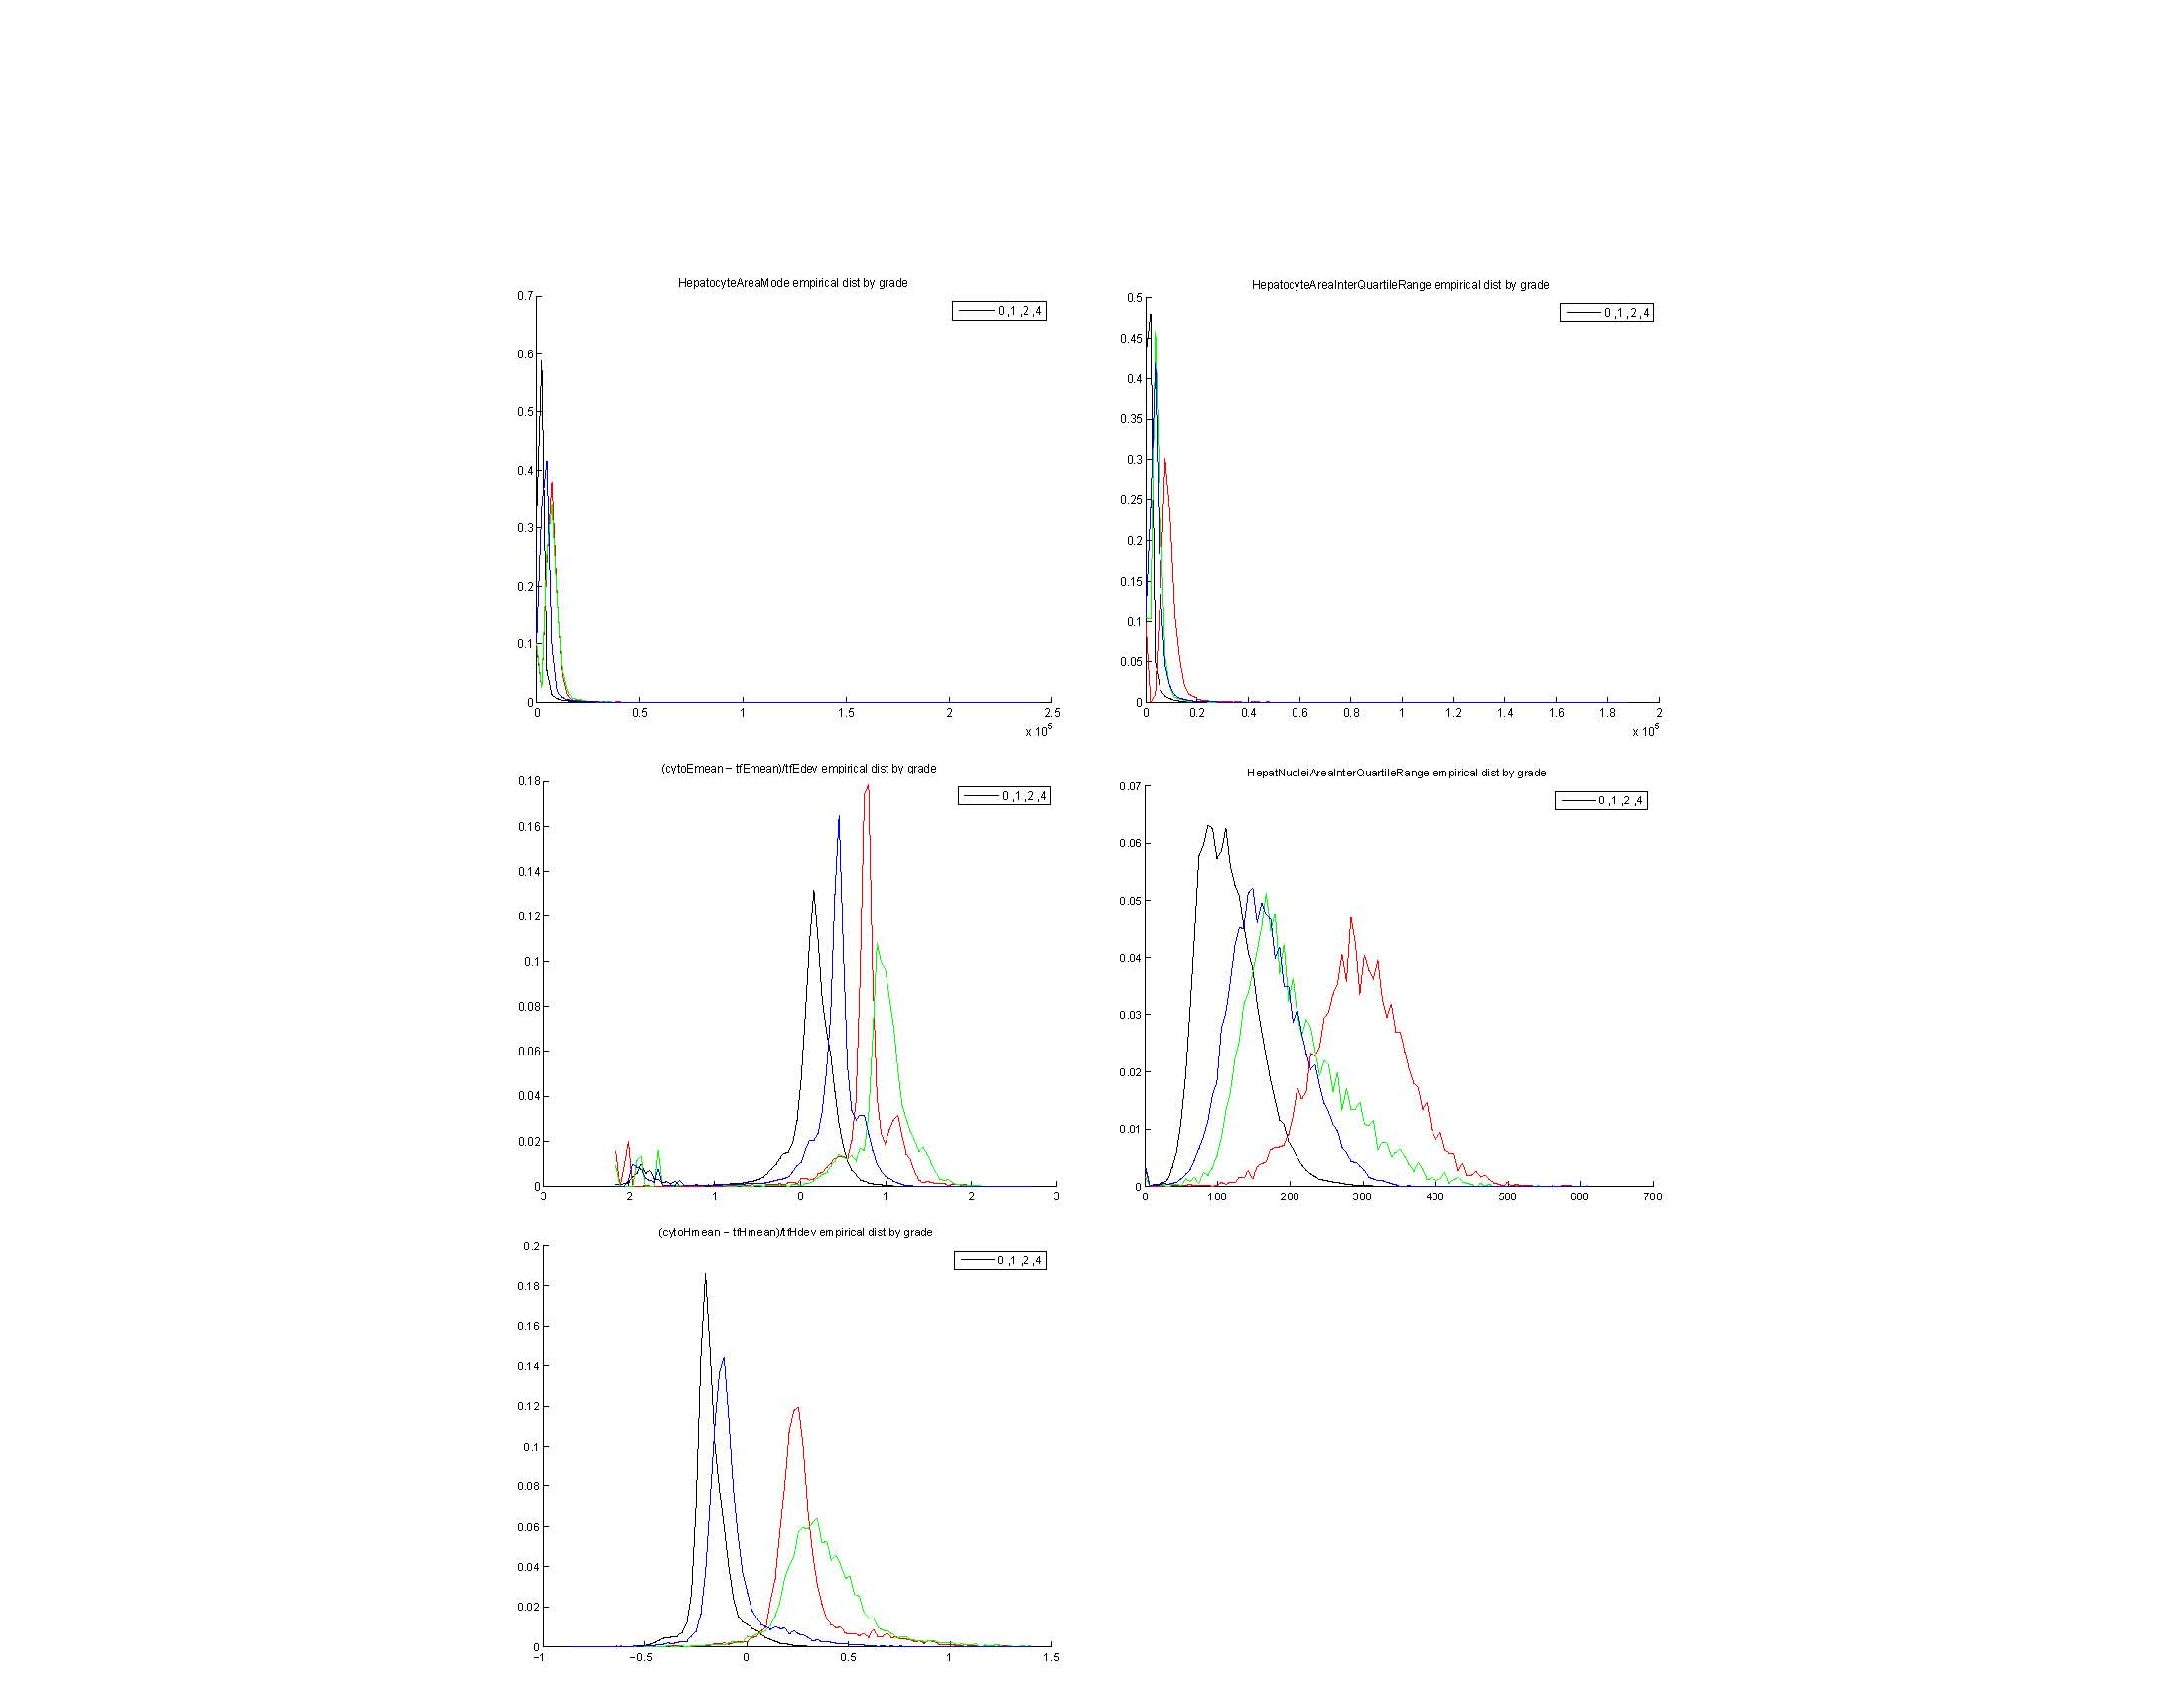
\includegraphics[width=5.0cm,height=5.0cm]{images/MachineVision/MachineVision_Pathology_ExampleSlides_Page_03.jpg} &
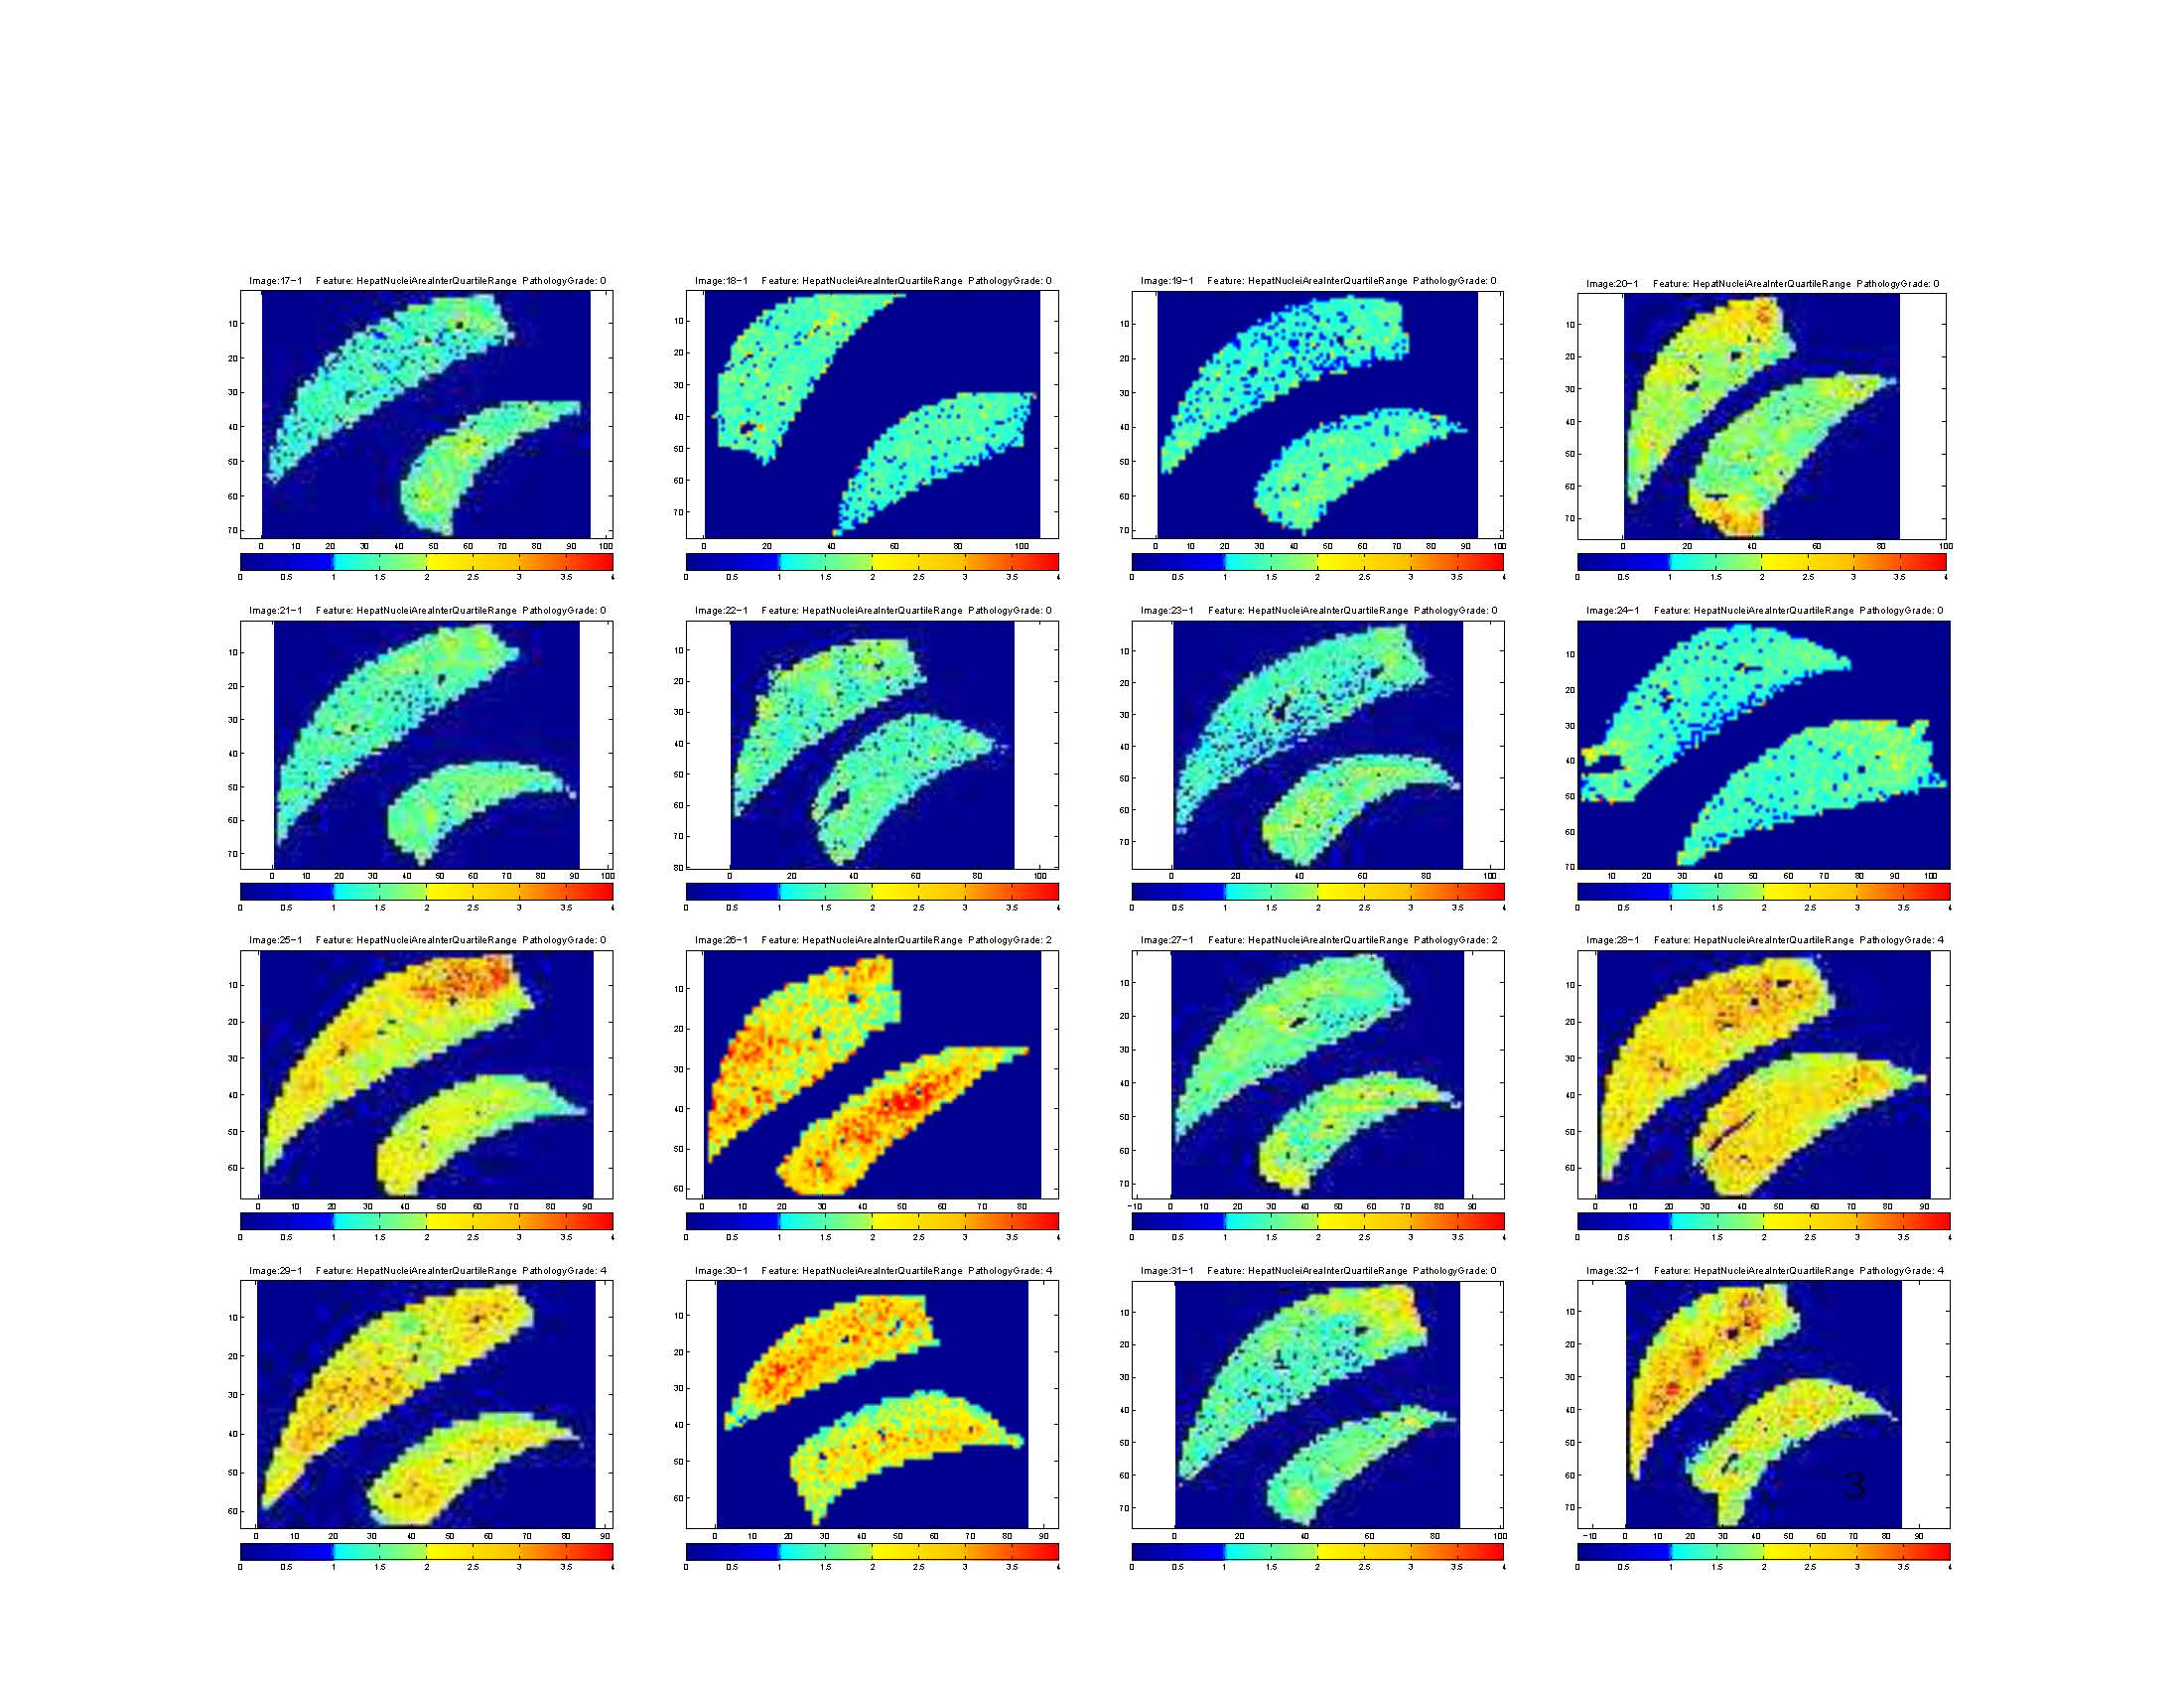
\includegraphics[width=5.0cm,height=5.0cm]{images/MachineVision/MachineVision_Pathology_ExampleSlides_Page_05.jpg} &
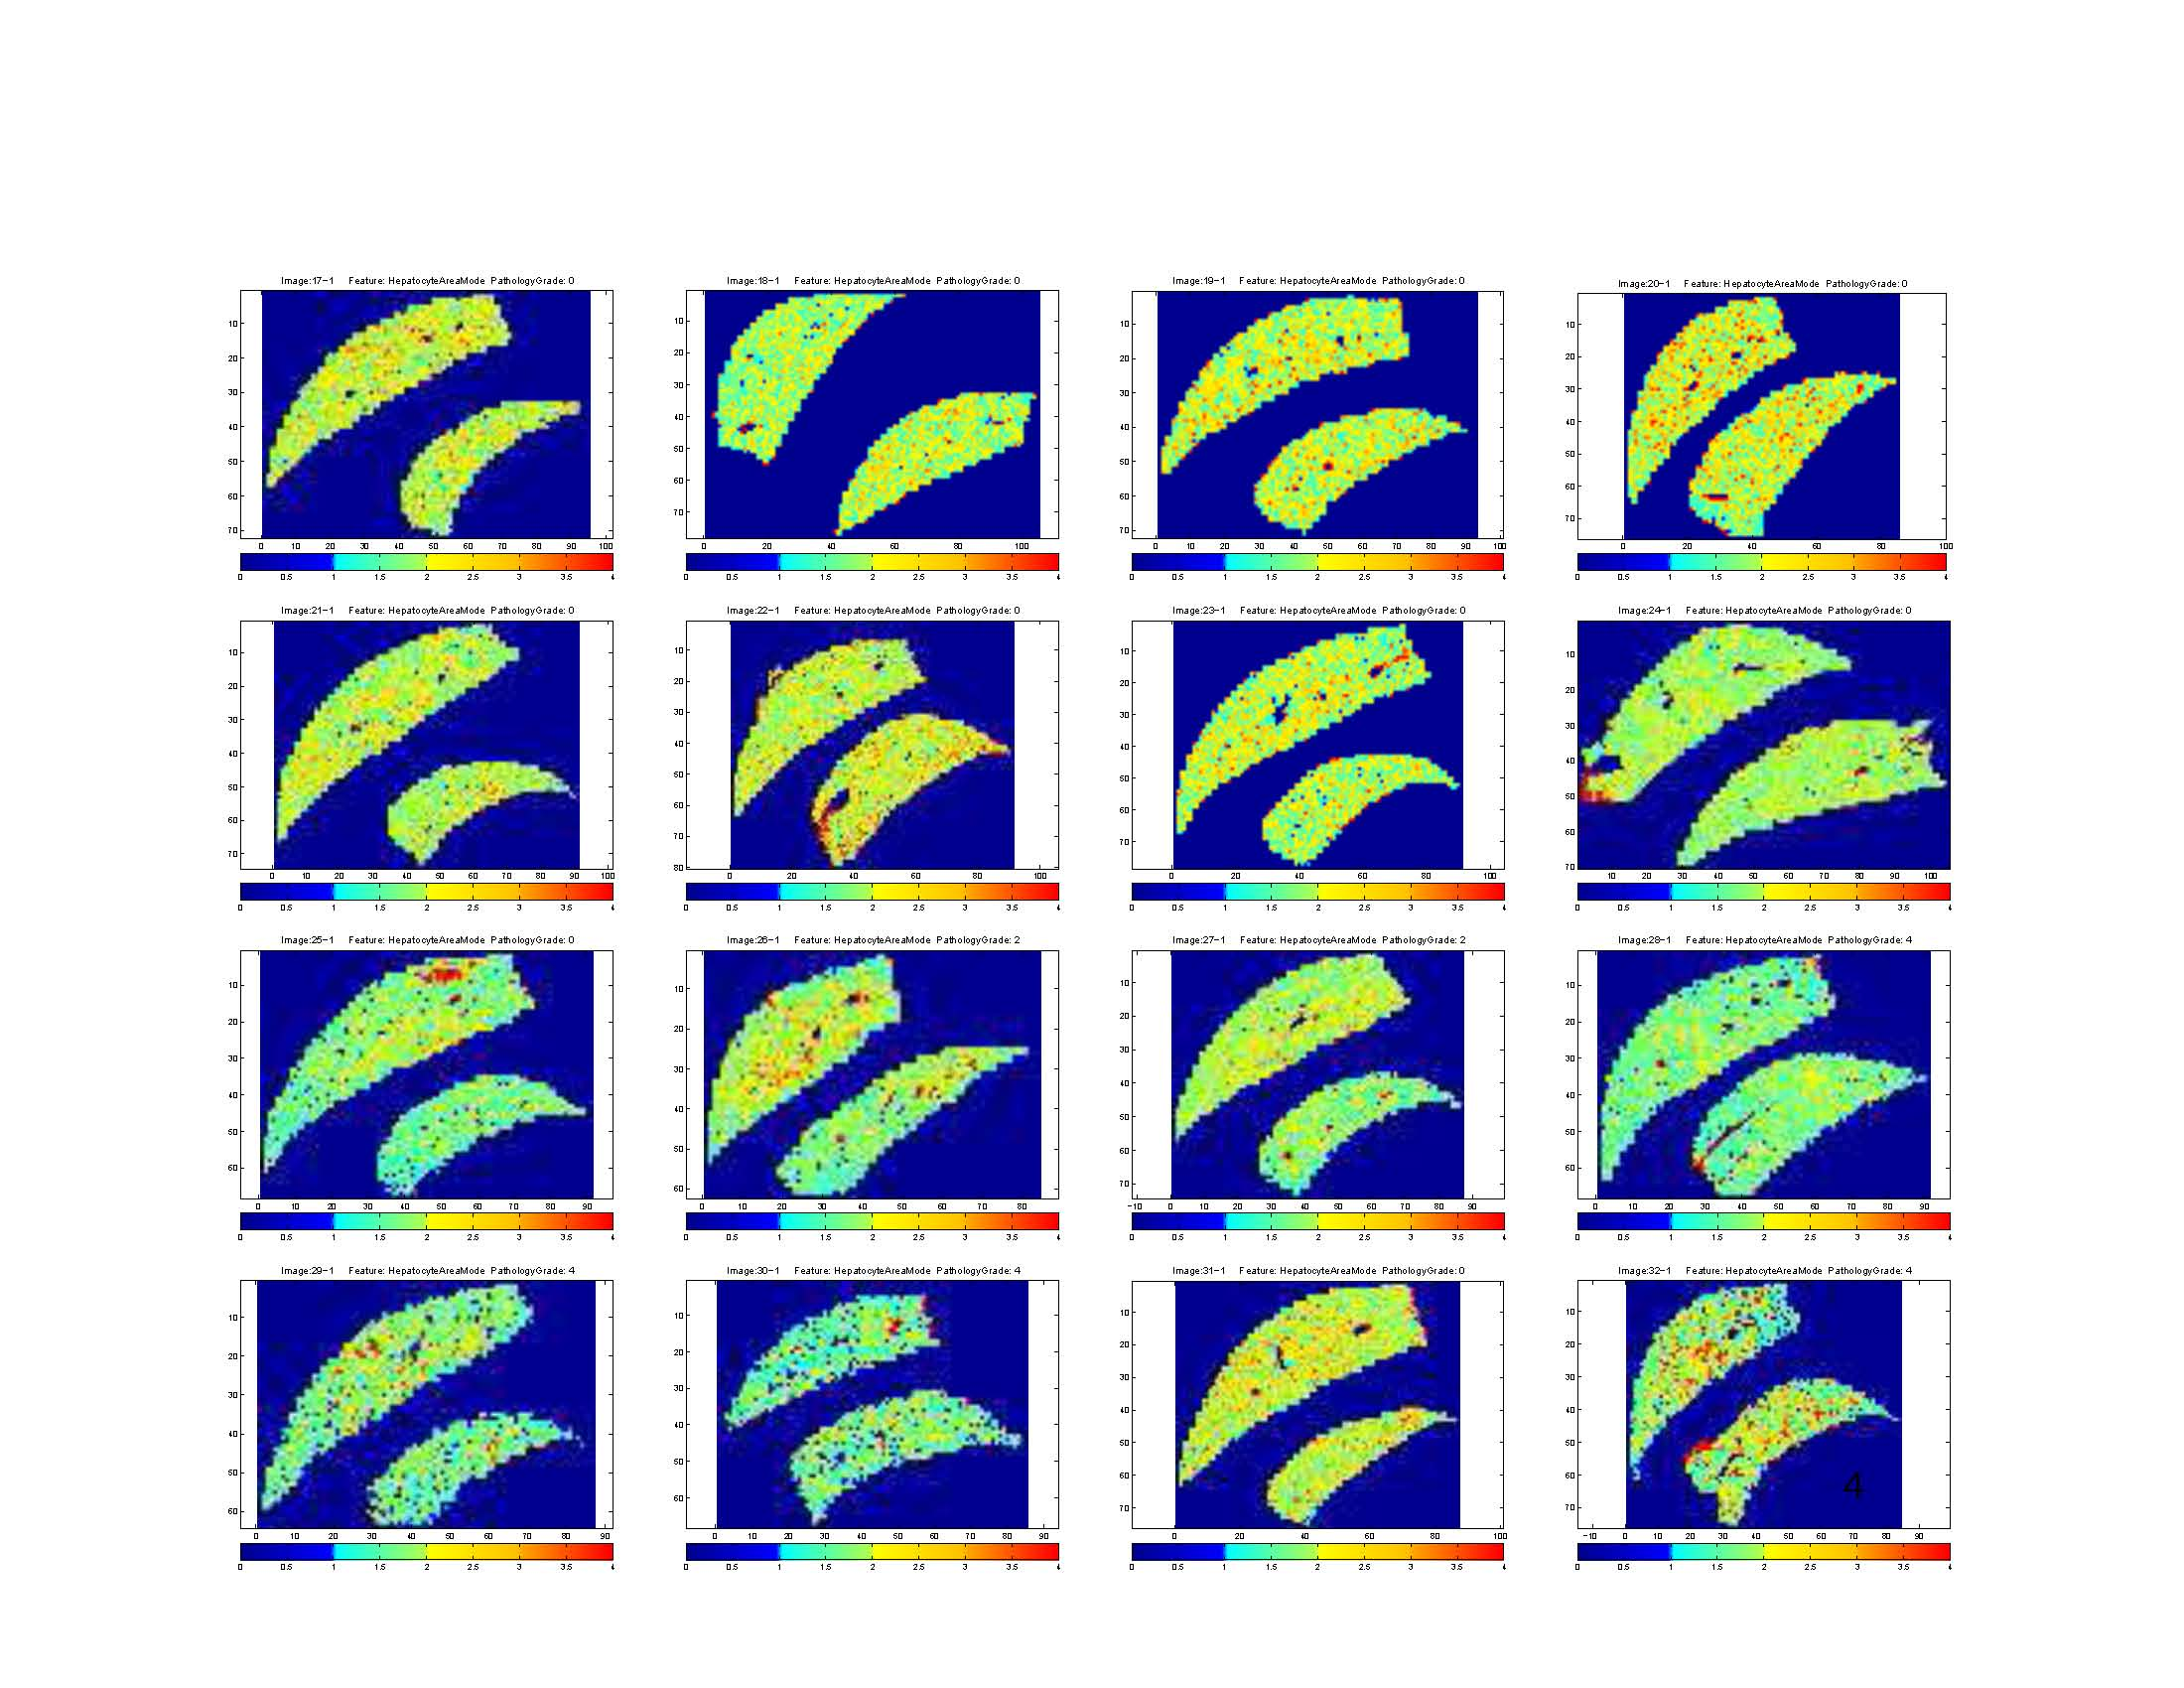
\includegraphics[width=5.0cm,height=5.0cm]{images/MachineVision/MachineVision_Pathology_ExampleSlides_Page_06.jpg} \\
\includegraphics[width=5.0cm,height=5.0cm]{images/MachineVision/MachineVision_Pathology_ExampleSlides_Page_07.jpg} &
\includegraphics[width=5.0cm,height=5.0cm]{images/MachineVision/MachineVision_Pathology_ExampleSlides_Page_08.jpg} &
\includegraphics[width=5.0cm,height=5.0cm]{images/MachineVision/MachineVision_Pathology_ExampleSlides_Page_09.jpg} \\
\includegraphics[width=5.0cm,height=5.0cm]{images/MachineVision/MachineVision_Pathology_ExampleSlides_Page_11.jpg} &
\includegraphics[width=5.0cm,height=5.0cm]{images/MachineVision/MachineVision_Pathology_ExampleSlides_Page_13.jpg} &
\includegraphics[width=5.0cm,height=5.0cm]{images/MachineVision/MachineVision_Pathology_ExampleSlides_Page_15.jpg} \\
\includegraphics[width=5.0cm,height=5.0cm]{images/MachineVision/MachineVision_Pathology_ExampleSlides_Page_16.jpg}
\end{tabular}


\begin{tabular}{ |c|c|c| }
\includegraphics[width=5.0cm,height=5.0cm]{images/Her2Fish/1_abConvexHull.jpg}  &
\includegraphics[width=5.0cm,height=5.0cm]{images/Her2Fish/1_Processedlabelimage.jpg}   &
\includegraphics[width=5.0cm,height=5.0cm]{images/Her2Fish/1_RGBMASK.jpg}  \\
\includegraphics[width=5.0cm,height=5.0cm]{images/Her2Fish/1_RGB_LabelImg.jpg}  &
\includegraphics[width=5.0cm,height=5.0cm]{images/Her2Fish/1_SampleChromas.jpg}  &
\includegraphics[width=5.0cm,height=5.0cm]{images/Her2Fish/2_abConvexHull.jpg}   \\
\includegraphics[width=5.0cm,height=5.0cm]{images/Her2Fish/2_Processedlabelimage.jpg}  &
\includegraphics[width=5.0cm,height=5.0cm]{images/Her2Fish/2_RGBMASK.jpg}           &
\includegraphics[width=5.0cm,height=5.0cm]{images/Her2Fish/2_RGB_LabelImg.jpg}   \\
\includegraphics[width=5.0cm,height=5.0cm]{images/Her2Fish/2_SampleChromas.jpg}   &
\includegraphics[width=5.0cm,height=5.0cm]{images/Her2Fish/3.jpg}
\end{tabular}


\begin{tabular}{ |c|c|c| }
\includegraphics[width=5.0cm,height=5.0cm]{images/Her2Fish/3_abConvexHull.jpg} \\
\includegraphics[width=5.0cm,height=5.0cm]{images/Her2Fish/3_BlueMaskOpen.jpg}   &
\includegraphics[width=5.0cm,height=5.0cm]{images/Her2Fish/3_RGB_LabelImg.jpg}    &
\includegraphics[width=5.0cm,height=5.0cm]{images/Her2Fish/3_SampleChromas.jpg}  \\
\includegraphics[width=5.0cm,height=5.0cm]{images/Her2Fish/4.jpg}               &
\includegraphics[width=5.0cm,height=5.0cm]{images/Her2Fish/4_RGB_LabelImg.jpg}  &
\includegraphics[width=5.0cm,height=5.0cm]{images/Her2Fish/B31-1677A108_ProcessedlabelimageWithSpotsEnhanced.jpg}  \\
\includegraphics[width=5.0cm,height=5.0cm]{images/Her2Fish/B31-1677A108_ProcessedlabelimageWithSpotsEnhanced2.jpg}  &
\includegraphics[width=5.0cm,height=5.0cm]{images/Her2Fish/B31-1677A108_ProcessedlabelimageWithSpotsEnhanced3.jpg}
\end{tabular}





\includegraphics[width=9.0cm,height=9.0cm]{images/GraphTheory/3Inhomog_Cluster_PreScaleFree.jpg}
\includegraphics[width=9.0cm,height=9.0cm]{images/GraphTheory/Clique_12_Members.jpg}
\includegraphics[width=9.0cm,height=9.0cm]{images/GraphTheory/Clique_3_Members.jpg}
\includegraphics[width=9.0cm,height=9.0cm]{images/GraphTheory/Clique_4_Members.jpg}
\includegraphics[width=9.0cm,height=9.0cm]{images/GraphTheory/Clique_5_Members.jpg}
\includegraphics[width=9.0cm,height=9.0cm]{images/GraphTheory/Clique_6_Members.jpg}
\includegraphics[width=9.0cm,height=9.0cm]{images/GraphTheory/Clique_9_Members.jpg}
\includegraphics[width=9.0cm,height=9.0cm]{images/GraphTheory/ClusterCoeff_Hist_ErdoReyani_Graph_SameVertexSet_mean0_421961099815438.jpg}
\includegraphics[width=9.0cm,height=9.0cm]{images/GraphTheory/ClusterCoeff_Hist_PreScaleFree_mean_0_205047904366710.jpg}
\includegraphics[width=9.0cm,height=9.0cm]{images/GraphTheory/ClusterCoeff_Hist_ScaleFree_with20ExtraNode_5maxE_mean_0_190053489673149.jpg}
\includegraphics[width=9.0cm,height=9.0cm]{images/GraphTheory/CVX_NNMF_A-YX_Where_Y_X_PSD.jpg}
\includegraphics[width=9.0cm,height=9.0cm]{images/GraphTheory/CVX_NNMF_A.jpg}
\includegraphics[width=9.0cm,height=9.0cm]{images/GraphTheory/CVX_NNMF_Residuals.jpg}
\includegraphics[width=9.0cm,height=9.0cm]{images/GraphTheory/Eigenvalues_of_Whshart_Follow_TracyWidom.jpg}
\includegraphics[width=9.0cm,height=9.0cm]{images/GraphTheory/ErdosReyni_G_LT_giant_thresh_.jpg}
\includegraphics[width=9.0cm,height=9.0cm]{images/GraphTheory/gursoy_atun_layou_topology_heart.jpg}
\includegraphics[width=9.0cm,height=9.0cm]{images/GraphTheory/hypercube_3_Dimension.jpg}
\includegraphics[width=9.0cm,height=9.0cm]{images/GraphTheory/hypercube_4_Dimension.jpg}
\includegraphics[width=9.0cm,height=9.0cm]{images/GraphTheory/hypercube_5_Dimension.jpg}
\includegraphics[width=9.0cm,height=9.0cm]{images/GraphTheory/hypercube_6_Dimension.jpg}
\includegraphics[width=9.0cm,height=9.0cm]{images/GraphTheory/hypercube_7_Dimension.jpg}
\includegraphics[width=9.0cm,height=9.0cm]{images/GraphTheory/hypercube_8_Dimension.jpg}
\includegraphics[width=9.0cm,height=9.0cm]{images/GraphTheory/RandomGraphAdjacencyMatrix_WithCut_jpg.jpg}
\includegraphics[width=9.0cm,height=9.0cm]{images/GraphTheory/RandomGraphOptimalEdgeInputGraph_AdjacencyMatrix.jpg}
\includegraphics[width=9.0cm,height=9.0cm]{images/GraphTheory/RandomGraphOptimalEdgeInputGraph_EdgeWeightHist_FMMC.jpg}
\includegraphics[width=9.0cm,height=9.0cm]{images/GraphTheory/RandomGraphOptimalEdgeInputGraph_IncidenceMatrix.jpg}
\includegraphics[width=9.0cm,height=9.0cm]{images/GraphTheory/RandomGraphOptimalEdgeWithedgeWeight_FastMixingMarkovChain.jpg}
\includegraphics[width=9.0cm,height=9.0cm]{images/GraphTheory/RandomGraphOptimalEdgeWithedgeWeight_PositiveTransitionProbs_FastMixingMarkovChain.jpg}
\includegraphics[width=9.0cm,height=9.0cm]{images/GraphTheory/RandomGraph_With3Cuts_.jpg}
\includegraphics[width=9.0cm,height=9.0cm]{images/GraphTheory/RandomGraph_With3Cuts_90_nodes_pii_25_pij_06.jpg}
\includegraphics[width=9.0cm,height=9.0cm]{images/GraphTheory/RandomGraph_With3Cuts_90_nodes_pii_25_pij_06_Adjacency_Matrix.jpg}
\includegraphics[width=9.0cm,height=9.0cm]{images/GraphTheory/RandomGraph_With3Cuts_90_nodes_pii_25_pij_06_Adjacency_Matrix_Minimized_PF.jpg}
\includegraphics[width=9.0cm,height=9.0cm]{images/GraphTheory/RandomGraph_With3Cuts_90_nodes_pii_25_pij_06_MinimizedAdjacency_PerronFrobenius.jpg}
\includegraphics[width=9.0cm,height=9.0cm]{images/GraphTheory/RandomGraph_WithCut_64Nodes.jpg}
\includegraphics[width=9.0cm,height=9.0cm]{images/GraphTheory/RandomGraph_WithCut_adjacencyMatrix_64Nodes.jpg}
\includegraphics[width=9.0cm,height=9.0cm]{images/GraphTheory/RandomGraph_WithCut_jpg.jpg}
\includegraphics[width=9.0cm,height=9.0cm]{images/GraphTheory/RandomWalk_30_Walkers_20000_steps.jpg}
\includegraphics[width=9.0cm,height=9.0cm]{images/GraphTheory/RandomWalk_50_Walkers.jpg}
\includegraphics[width=9.0cm,height=9.0cm]{images/GraphTheory/Raymond_AdvectiveNavierStokesdiffusion.jpg}
\includegraphics[width=9.0cm,height=9.0cm]{images/GraphTheory/Raymond_TensorField.jpg}
\includegraphics[width=9.0cm,height=9.0cm]{images/GraphTheory/RoadMap.jpg}
\includegraphics[width=9.0cm,height=9.0cm]{images/GraphTheory/WellConnectedWithRedBlackOrder_Bipatate.jpg}
\includegraphics[width=9.0cm,height=9.0cm]{images/GraphTheory/WellConnectedWithThreeClusters.jpg}
\includegraphics[width=9.0cm,height=9.0cm]{images/GraphTheory/WellConnectedWithThreeClusters2.jpg}
\includegraphics[width=9.0cm,height=9.0cm]{images/GraphTheory/WellConnectedWithThreeClusters3.jpg}
\includegraphics[width=9.0cm,height=9.0cm]{images/GraphTheory/WishartMatrixforMikey.jpg}
\includegraphics[width=9.0cm,height=9.0cm]{images/GraphTheory/_GtDout.jpg}

%\chapter{Natural Language Processing}

\includegraphics[width=5.0cm,height=5.0cm]{wordassociation.jpg} 
A word association graph using the based on the WordNet database. 

\section{Introduction}
This document is primarily meant to server as a brief tutorial to Natural Language Processing (NLP) as it applies to the problems of classification and prediction of text.  The statistical part comes from the use of corpora and probabilistic models in prediction and classification.  Computational linguistics is an interdisciplinary field dealing with the statistical and/or rule-based modeling of natural language from a computational perspective.  Computational linguistics is primarily concerned with developing algorithms and software for intelligently processing language data and is typically views as a subset of AI.  For our purposes we refer to classification as the process of estimating a categorical variable and prediction as the process of estimating a continuous variable.  For example , assigning a probability for the next word in a string of words is classification, while assigning a vulgarity index to a string of words is regarded as prediction.  A canonical open problem in Computational Linguistics is the automatic translation of one language into another, a task which requires understanding the morphological and syntactical structure of both languages. Other problems in this field include :
\begin{center}
\begin{itemize}
  \item Computational complexity of natural language
  \item Computational semantics
  \item Computer-aided corpus linguistics
  \item Development of parsers for natural languages
  \item Development of taggers to identify parts of speech
  \item Word Sense Disambiguation
\end{itemize}
\end{center}
Some specific problems this document is concerned with are:
\begin{itemize}
  \item Word Completion.  Given a sequence of letters, find the word that best completes the sequence.
  \item Word Prediction. Given a sequence of words, find the word that best completes the sequence.
  \item Document \& Text Classification.
\end{itemize}

While we are primarily interested in a statistical approach to natural language processing, a basic to understanding of syntax and semantics is required to handle the many 'outlier' cases one will encounter.  Modern English has many exceptional rules that must be dealt with.  This document contains two appendices with definitions that reader will want to be familiar with.  Two important tasks in NLP are the decoding of syntactic and semantic information.  These are discussed broadly below.

\subsection{Semantics}
Linguistic semantics refers to the meanings that language elements express.  It typically focuses on the relation between signifiers, such as words, phrases, signs and symbols, and what they stand for.  The term is used in ordinary language to denote a problem of understanding that comes down to word selection or connotation. In written language, such things as paragraph structure and punctuation have semantic content.  The basic unit of semantics is sense.  One word may have many different meanings.  Deriving the meaning from a context - called word sense disambiguation - is a key task in computational linguistics.

\subsection{Lexicography}Lexicography is divided into two related disciplines, practical and theoretical.  Practical lexicography is the art or craft of compiling, writing and editing dictionaries.  Theoretical lexicography is the scholarly discipline of analyzing and describing the semantic, syntagmatic and paradigmatic relationships within the lexicon (vocabulary) of a language, developing theories of dictionary components and structures linking the data in dictionaries, the needs for information by users in specific types of situation, and how users may best access the data incorporated in printed and electronic dictionaries.

\subsection{Corpus linguistics} Corpus linguistics is the study of language as expressed in samples (corpora) or "real world" text. This method represents a digestive approach to deriving a set of abstract rules by which a natural language is governed or else relates to another language. Originally done by hand, corpora are now largely derived by an automated process.


\section{A Quantification the Semantic Information in WordNet}
 WordNet \cite{WORDNET} is a lexical database for the English language. It groups English words into sets of synonyms called synsets, provides short, general definitions, and records the various semantic relations between these synonym sets.  We are interested analyze the statistics of the WordNet semantic graph with the aim to inject sematic information into statistical models.  A "semantic sweetenting" of sorts.

\section{N-gram Models}
N-grams are an important part of NLP tasks like tagging parts of speech, natural language generation [chatterbot engines], plagiarism identification, and character prediction in cell phone text input.  To get an idea of how an  n-gram model is built we will use example n-grams extracted from Anna Kerannina [AK].  The phrase \emph{"for the first time"}, a 4-gram, appears 27 times the body of the novel:
\begin{tiny}
\begin{itemize}
\item saw \emph{for the first} time that inner life of an old, noble,
\item and to make her an offer.  And only then \emph{for the first time} the
\item In Moscow he had \emph{for the first time} felt, after his luxurious and
\item \emph{for the first time} did Vronsky realize clearly the fact that
\item seeing her \emph{for the first time} with all her defects.
\item him \emph{for the first time}.  She was conscious herself that her
\item \emph{For the first time} the question presented itself to him of the
\item feeling.  \emph{For the first time} he pictured vividly to himself her
\item Levin put on his big boots, and, \emph{for the first time}, a cloth
\item And \emph{for the first time} the idea clearly presented itself that it
\item he was going.  He felt utterly wretched.  \emph{For the first time} in
\item mowing this summer \emph{for the first time}.
\item of the men who led this life; but today \emph{for the first time},
\item eagerness, recollecting her son's existence \emph{for the first time}
\item his nose, and \emph{for the first time} in his life he felt on the point
\item death.  Death, the inevitable end of all, \emph{for the first time}
\item moment.  And \emph{for the first time}, for an instant, she felt for
\item with him or separately, that \emph{for the first time} he clearly
\item Now \emph{for the first time} he heard her words with pleasure, and did
\item Vronsky \emph{for the first time} experienced a feeling of anger against
\item Vassenka Veslovsky, obviously \emph{for the first time} in his life
\item "And here we've met \emph{for the first time} since we met at your
\item Jew, or that \emph{for the first time} in his life he was not following
\item talk which he was hearing \emph{for the first time}.  The complexity of
\item it."  And now \emph{for the first time} Anna turned that glaring light
\item for a muslin garment, and going \emph{for the first time} into the frost
\item Then, \emph{for the first time}, grasping that for every man, and
\end{itemize}
\end{tiny}
There are 14200 unique words in the text and 368588 words total.  The frequencies of the unigrams are
{for 2636, the 16579, first 348, time 564}
The unigram \emph{for} appears 2636 times.
The bigram \emph{for the} appears 433 times.
The trigram \emph{for the first} appears 48 times.

We'll come back to these numbers in a moment. Frequencies of the n-grams are presented along with the text in the sequel.

First we need to discuss a subtlety in predicting text.  The two strings \emph{for the} and \emph{for the } are very different when it comes to predicting what comes next.  The bigrams that match the latter in our example text are
\emph{{for the 433, for them 36, for their 21,for these 6,for themselves 6,for they 3, for theirs 1}}
Where there is only one possible bigram matching the former string. Intra word  prediction requires unigram frequencies. The possible matches for continuing \emph{the} are {the 16576, they 998, there 965,them 841,their 689,then 410} We use these counts to define conditional probabilities of the form:
\begin{eqnarray*}
P("the" | "the ") =1 \\
P("the" | "the") = 16579/(16579+998+841+689+401) \\
P("they" | "the" = 998/(16579+998+841+689+401)
\end{eqnarray*}
We refer to the conditional $g$ in $P(w|g)$ as the context, $ g= (w_{1}, ...,w_{i},...,w_{n})$  Using the chain rule this is broken into a product of conditional probabilities,

\begin{eqnarray*}
P(w_{1}, ...,w_{i},...,w_{n}) = P(w_{n}|w_{1} ...,w_{i},...,w_{n-1}) * P(w_{1}, ...,w_{i},...,w_{n-1}) \\
 = P(w_{n}|w_{1} ...,w_{i},...,w_{n-1}) * P(w_{n-1}|w_{1} ...,w_{i},...,w_{n-2}) * P(w_{1}, ...,w_{i},...,w_{n-2})\\
\ldots \\
= P(w_{1}) * P(w_{2} | w_{1}) * P(w_{3} | w_{1} w_{2}) ... P(w_{n} | w_{2} ...w_{n-1})
\end{eqnarray*}
The conditional probabilities are computed using n-grams;
\begin{itemize}
\item unigram $P(w_{i} | g) = P(w_{i})$ \\
\item bigram  $P(w_{i} | g) = P(w_{i} | w_{i-1})$ \\
\item trigram $P(w_{i} | g) =  P(w_{i} | w_{i-1} w_{i-2})$
\end{itemize}
and so forth.  Estimates are obtained from n-gram frequency counts in a training corpus.
to compute the unigram conditional probabilities, $P(w) =  \frac{card(w) }{N}$ Where $N$ is the total number of tokens in the corpus. Bigram conditionals are computed likewise, except that we normalize by the total number of bigrams with the first word $P(w_{i} | w_{i-1}) =  \frac{card( (w_{i-1},w_{i}) ) }{\sum\limits_{w_{n} \in B} card( (w_{i-1},w_{n}))}$

We can calculate the conditionals with our test corpus.  We use $*$ as a wild card.

\[P(for, the, first, time) = P(for)  P(the | for)  P(first | for, the)  P(time | for, the, first)\]

\[P(for, the, first, time) =  \frac{the=16576}{words-368588}  \frac{for, the =433}{for, * = 2663} \frac{for, the, first =48}{for, the * = 433}  \frac{for, the, first, time  =31}{for, the, first, * = 48} \]

\[P(for, the, first, time) =  0.0005235149\]


$P(for the first time)$ as calculated above is bigger than the ratio of \emph{for the first time} to all quad-grams $31/342132 = .0000906083$


\section{Appendix : Syntax}
Syntax is the rule set for constructing sentences in natural languages.  The word is the smallest unit of syntactical structure and a related to each other through rules of grammar.  Traditionally, grammar and syntax dictate that every sentence has a subject and predicate that form the nuclear part of a sentence  The parts of a sentence decorating subject and predicate are termed extranuclear.
There are eight traditional parts of speech (POS) in the English language:
\begin{itemize}
  \item Verb : action or state \emph{Buddha \textbf{climbed} the wall.}
  \item Noun : thing or person \emph{jade}
  \item Adjective : describes a noun \emph{Nice jade Buddha}
  \item Adverb : describes a verb, adjective or adverb \emph{Buddha climbed slowly}
  \item Pronoun : replaces a noun
  \item Preposition : links a noun to another word
  \item Conjunction : joins clauses or sentences or words
  \item Interjection : short exclamation, sometimes inserted into a sentence
\end{itemize}

A more comprehensive POS list used in tagging, stemming, and inflecting text is presented below.
This is from the well known PENN database.  The Penn Treebank Project annotates naturally-occuring text for linguistic structure \cite{PENNTREEBANK}.
\begin{tiny}
\begin{tabular}{|c|c|}
  \hline
Coordinating conjunction	&	CC	\\
Cardinal number	&	CD	\\
Determiner	&	DT	\\
Existential there 	&	EX	\\
Foreign word	&	FW	\\
Preposition or subordinating conjunction	&	IN	 \\
Adjective	&	JJ	\\
Adjective, comparative	&	JJR	\\
Adjective, superlative	&	JJS	\\
List item marker	&	LS	\\
Modal	&	MD	\\
Noun, singular or mass	&	NN	\\
Noun, plural	&	NNS	\\
Proper noun, singular	&	NNP	\\
Proper noun, plural	&	NNPS	\\
Predeterminer	&	PDT	\\
Possessive ending	&	POS	\\
Personal pronoun	&	PRP	\\
Possessive pronoun	&	PRP\$	\\
Adverb	&	RB	\\
Adverb, comparative	&	RBR	\\
Adverb, superlative	&	RBS	\\
Particle	&	RP	\\
Symbol	&	SYM	\\
to	&	TO	\\
Interjection	&	UH	\\
Verb, base form	&	VB	\\
Verb, past tense	&	VBD	\\
Verb, gerund or present participle	&	VBG	\\
Verb, past participle	&	VBN	\\
Verb, non-3rd person singular present	&	VBP	\\
Verb, 3rd person singular present	&	VBZ	\\
Wh-determiner	&	WDT	\\
Wh-pronoun	&	WP	\\
Possessive wh-pronoun	&	WP\$	\\
Wh-adverb	&	WRB	\\
  \hline
\end{tabular}
\end{tiny}

One will generally encounter rule-sets to transform between parts of speech in stemming and inflection engines.


\begin{small}
\subsection{Grammatical Syntactic Definitions}
\subsubsection{adjective}
An adjective is a word whose main syntactic role is to modify a noun or pronoun, giving more information about the noun or pronoun's referent. The adjective order in English is:
\begin{center}
\begin{itemize}
  \item article or pronouns used as adjectives
  \item quality
  \item size
  \item age
  \item shape
  \item color
  \item proper adjective (often nationality or other place of origin)
  \item purpose or qualifier
\end{itemize}
\end{center}
One of the syntactic rules for English prescribes that adjectives describing size precede adjectives pertaining to age.  Another syntactic rule for adjective is that adjectives describing color come after shape. Thus the phrase \emph{"My poor fat old round *"} is a well formed phrase while \emph{"My old square red *"} is not.

\subsubsection{adjunct}
 Adjuncts are optionally omissible parts of a sentence that do not affect the remainder when removed. The sentence: \emph{I won the bike race in the park while it was raining last Saturday}.  Has adjuncts \emph{in the park}, \emph{ while it was raining}, and \emph{last Saturday}.

\subsubsection{adverb}
An adverb is a modifying part of speech describing verbs, other adverbs, adjectives, and phrases. They are used to describe how, where, when, how often, and why something happens.
Adverbs of manner:  \emph{carefully, correctly, eagerly, easily, fast, loudly, patiently,  quickly, quietly, and well}.

Adverbs of place: \emph{abroad, anywhere, downstairs, here, home, in, nowhere, out, outside, somewhere, there, underground, upstairs}.

Adverbs of purpose : \emph{so, so that, to, in order to, because, since, accidentally, intentionally, purposely}.

Adverbs of frequency: \emph{always, every ,never ,often, rarely ,seldom, sometimes, usually}.

Adverbs of time : \emph{after, already, during, finally, just, last, later, next, now, recently, soon}

Adverbs of manner are usually formed by adding \emph{ly} to adjectives. Softly comes from soft, usually come from usual.  The suffix \emph{wise} and \emph{ways} may be used to derive adverbs from nouns. Some adverbs are formed from nouns or adjectives by appending the prefix \emph{a}. There are a number of other suffixes in English that derive adverbs from other word classes, and there are also many adverbs that are not morphologically indicated at all.  Adverbs in English are inflected in terms of comparison like adjectives. The comparative and superlative forms of some single-syllable adverbs that do not end in \emph{ly} are generated by adding \emph{er} and \emph{es}t . Others, especially those ending \emph{ly}, are periphrastically compared by the use of more or most -- while some accept both forms, e.g. oftener and more often are both correct. Adverbs also take comparisons with as ... as, less, and least.  Not all adverbs are comparable; for example in the sentence \emph{He wore red yesterday} it does not make sense to speak of "\emph{more yesterday}" or "\emph{most yesterday}".

\subsubsection{appositive}Apposition is a grammatical construction in which two elements, normally noun phrases, are placed side by side, with one element serving to define or modify the other. When this device is used, the two elements are said to be in apposition. For example, in the phrase \emph{my friend Alice} the name \emph{Alice} is in apposition to \emph{my friend}.  Apposition is a figure of speech of the scheme type, and often results when the verbs (particularly verbs of being) in supporting clauses are eliminated to produce shorter descriptive phrases. This makes them often function as hyperbatons, or figures of disorder, because they can disrupt the flow of a sentence. For example, in the phrase: \emph{My dog, a Papillon with big ears,...}, it is necessary to pause before the parenthetical modification \emph{Papillon with big ears}.

\subsubsection{article}
An article is a word that combines with a noun to indicate the type of reference being made by the noun. Articles specify the grammatical definiteness of the noun, in some languages extending to volume or numerical scope. English articles are \emph{the, and, a, an}.  The word \emph{some} is used as a functional plural of \emph{a, an}.  Articles are considered a special category of adjectives.
Generally common nouns are expressed as definite or indefinite and singular or plural. Every noun must be accompanied by the article, if any, corresponding to its definiteness, and the lack of an article (considered a zero article) itself specifies a certain definiteness. This is in contrast with optional adjectives and determiners.  The compulsory nature of articles makes them the most frequently use words.

\subsubsection{aspect}
The grammatical aspect  of a verb is a grammatical category that defines the temporal flow, or lack thereof, in a given action, event, or state (in a given situation). Commonly the distinction is in how the speaker views the situation, either as unitary and bounded \emph{I ate} or as on-going and unbounded \emph{I was eating}. The distinction here is not in the situation itself, but in the speaker's portrayal of it. Other common aspectual distinctions include whether the situation is repetitive or habitual \emph{I used to eat} or has continuing relevance \emph{I have eaten}. Any one language will have at most a subset of the attested aspectual distinctions made in the world's languages.  Aspect can be a difficult concept to convey and understand intuitively. Because they both convey some sense of time, aspect is often confused with the closely-related concept of tense. While tense relates the time of a situation to some other time, commonly the time of speaking, aspect conveys other temporal information, such as duration, completion, or frequency, as it relates to the time of action. Thus tense refers to temporally when while aspect refers to temporally how. Aspect can be said to describe the texture of the time in which a situation occurs, such as a single point of time, a continuous range of time, a sequence of discrete points in time, etc, whereas tense indicates its location in time.  The concept of aspect is best illustrated by example. Consider the following sentences: \emph{I eat}, \emph{I am eating}, \emph{I have eaten}, and \emph{I have been eating}. All are to some degree in the present tense, as they describe the present situation, yet each conveys different information or points of view as to how the action pertains to the present. As such, they differ in aspect.

\subsubsection{auxiliary verb}
An auxiliary is a verb functioning to give further semantic or syntactic information about the main or full verb following it.  An auxiliary verb alters the basic form of the main verb to make it have one or more of the following functions: passive voice, progressive aspect, perfect aspect, modality, or dummy.
Every clause has a finite verb which consists of a full verb non-auxiliary and optionally one or more auxiliary verbs.
Examples of finite verbs include \emph{write} (no auxiliary verb), \emph{have written} (one auxiliary verb), and \emph{have been written} (two auxiliary verbs).  The primary auxiliary verbs in English are \emph{to be} and \emph{to have}; other major ones include \emph{shall}, \emph{will}, \emph{may} and \emph{can}.

\subsubsection{case}
The case of a noun or pronoun is a change in form that indicates its grammatical function in a phrase, clause, or sentence.  For example, a noun may play the role of subject \emph{I kicked the ball}, of direct object \emph{John kicked me}, or of possessor \emph{My ball}.  More formally, case has been defined as a system of marking dependent nouns for the type of relationship they bear to their heads.

\subsubsection{clause}
A clause is a pair or group of words that consists of a subject and a predicate, although in some languages and some types of clauses the subject may not appear explicitly as a noun phrase. It may instead be marked on the verb (this is especially common in null subject languages). The most basic kind of sentence consists of a single clause. More complicated sentences may contain multiple clauses, including clauses contained within clauses.  Clauses are often contrasted with phrases. Traditionally, a clause was said to have both a finite verb and its subject, whereas a phrase either contained a finite verb but not its subject (in which case it is a verb phrase) or did not contain a finite verb. Hence, in the sentence "I didn't know that the dog ran through the yard," "that the dog ran through the yard" is a clause, as is the sentence as a whole, while "the yard," "through the yard," "ran through the yard," and "the dog" are all phrases. However, modern linguists do not draw the same distinction, as they accept the idea of a non-finite clause, a clause that is organized around a non-finite verb.

\subsubsection{closed class word}
Closed class is a word class to which no new items can normally be added, and that usually contains a relatively small number of items. Typical closed classes found in many languages are adpositions (prepositions and postpositions), determiners, conjunctions, and pronouns.  Contrastingly, an open class offers possibilities for expansion. Typical open classes such as nouns and verbs can and do get new words often, through the usual means such as compounding, derivation, coining, borrowing, etc.  A closed class may get new items through these same processes, but the change takes much more time. The closed class is normally viewed as part of the core language and is not expected to change. Most readers can undoubtedly think of new nouns or verbs entering their lexicon, but it's very unlikely that they can recall any new prepositions or pronouns appearing in the same fashion

\subsubsection{comparative}The comparative is the form of an adjective or adverb which denotes the degree or grade by which a person, thing, or other entity has a property or quality greater or less in extent than that of another, and is used in this context with a subordinating conjunction, such as than, as...as, etc. If three or more items are being compared, the corresponding superlative needs to be used instead.
\subsubsection{complement}Complement is used with different meanings. The primary meaning is a word, phrase or clause which is necessary in a sentence to complete its meaning. We find complements which function as an argument (i.e. of equal status to subjects and objects) and complements which exist within arguments.  Both complements and modifiers add to the meaning of a sentence. However, a complement is necessary to complete a sentence; a modifier is not. For example, "Put the bread on the table" needs "on the table" to make it complete. In most dialects of English, you cannot merely put something; you need to put it somewhere. In this context, the phrase "on the table" is a complement. By contrast, "The bread on the table is fresh." does not require "on the table" to be complete, so here, the phrase "on the table" is a modifier. A modifier, unlike a complement, is an optional element of a sentence

\subsubsection{compound noun and adjective}
 A compound is a lexeme (less precisely, a word) that consists of more than one stem. Compounding or composition is the word formation that creates compound lexemes (the other word-formation process being derivation). Compounding or Word-compounding refers to the faculty and device of language to form new words by combining or putting together old words. In other words, compound, compounding or word-compounding occurs when a person attaches two or more words together to make them one word. The meanings of the words interrelate in such a way that a new meaning comes out which is very different from the meanings of the words in isolation.

\subsubsection{conjugation}Conjugation is the creation of derived forms of a verb from its principal parts by inflection (regular alteration according to rules of grammar). Conjugation may be affected by person, number, gender, tense, aspect, mood, voice, or other grammatical categories. All the different forms of the same verb constitute a lexeme and the form of the verb that is conventionally used to represent the canonical form of the verb (one as seen in dictionary entries) is a lemma. Inflection of nouns and adjectives is known as declension.  Conjugated forms of a verb are called finite forms. In many languages there are also one or more forms that remain unchanged with all or most of grammatical categories: the non-finite forms, such as the infinitive or the gerund. A table giving all the conjugated variants of a verb in a given language is called a conjugation table or a verb paradigm.  Although conjugation tables are a useful tool for the beginner in a foreign language, they fail in irregular verbs. This limitation is particularly prominent in Latin-derived languages like French and Italian. The availability of high power computers has made possible to replace the conjugation tables with conjugation algorithms, that can handle without difficulty the conjugation and the grammar analysis of any verb. However, these are much less useful in understanding the structure of the conjugation forms of a given language.  A regular verb has a set of conventions for conjugation (paradigm) that derives all forms from a few specific forms or principal parts (maybe only one, such as the infinitive in English), in spelling or pronunciation. A verb that has conjugations deviating from this convention is said to be an irregular verb. Typically the principal parts are the root and/or several modifications of it (stems).  Conjugation is also the traditional name of a group of verbs that share a similar conjugation pattern in a particular language (a verb class). This is the sense in which teachers say that Latin has four conjugations of verbs. This means that any regular Latin verb can be conjugated in any person, number, tense, mood, and voice by knowing which of the four conjugation groups it belongs to, and its principal parts

\subsubsection{conjunction}
A conjunction  is a part of speech that connects two words, phrases or clauses together. This definition may overlap with that of other parts of speech, so what constitutes a "conjunction" should be defined for each language. In general, a conjunction is an invariable grammatical particle, and it may or may not stand between the items it conjoins.

The definition can also be extended to idiomatic phrases that behave as a unit with the same function as a single-word conjunction (as well as, provided that, etc.).
1 Coordinating conjunctions
2 Correlative conjunctions
3 Subordinating conjunctions

Coordinating conjunctions, also called coordinators, are conjunctions that join two or more items of equal syntactic importance, such as words, main clauses, or sentences. In English the mnemonic acronym FANBOYS can be used to remember the coordinators \emph{for, and, nor, but, or, yet}, and \emph{so}. These are not the only coordinating conjunctions; various others are used, including \emph{and nor} (British), \emph{but nor} (British), \emph{or nor}(British), \emph{neither} as in \emph{They don't gamble; neither do they smoke}

\emph{for}: presents a reason \emph{He lost all his money, for he gambled too long}
\emph{and}: presents non-contrasting item(s) or idea(s)\emph{ They gamble, and they smoke.}
\emph{or}: presents an alternate item or idea \emph{Every day they gamble or they smoke.}
\emph{nor}: presents a non-contrasting negative idea \emph{They don't gamble, nor do they smoke.}
\emph{but}: presents a contrast or exception \emph{They gamble, but they don't smoke.}
\emph{yet}: presents a contrast or exception \emph{They gamble, yet they don't smoke.}
\emph{so}: presents a consequence \emph{He gambled too long, so he lost all his money.}
Correlative conjunctions are pairs of conjunctions that work together to coordinate two items. English examples include both and, [n]either [n]or, and not [only] but [also], whether... or.

Examples:
\emph{
Either do your work or prepare for a trip to the office.
Not only is he handsome but he is also brilliant.
Neither the basketball team nor the football team is doing well.
Both the cross country team and the swimming team are doing well.
}
\subsubsection{dangling modifier}
A dangling modifier, a specific case of which is the dangling participle, is an error in sentence structure whereby a grammatical modifier is associated with a word other than the one intended, or with no particular word at all. For example, a writer may have meant to modify the subject, but word order makes the modifier seem to modify an object instead. Such ambiguities can lead to unintentional humor or difficulty in understanding a sentence.  A typical example of a dangling modifier is illustrated in the sentence \emph{Turning the corner, a handsome school building appeared}. The modifying clause \emph{Turning the corner} is clearly supposed to describe the behavior of the narrator (or other observer), but grammatically it appears to apply to nothing in particular, or to the school building. Similarly, in the sentence \emph{At the age of eight, my family finally bought a dog}, the modifier \emph{At the age of eight} "dangles" in mid-air, attaching to no named person or thing.

\subsubsection{declension}
Declension is the inflection of nouns, pronouns, adjectives, and articles to indicate number (at least singular vs. plural), case (nominative or subjective, genitive or possessive, etc.), and gender.

\subsubsection{determiner}
A determiner is a noun-modifier that expresses the reference of a noun or noun-phrase in the context, rather than attributes expressed by adjectives. This function is usually performed by articles, demonstratives, possessive determiners, or quantifiers.
\emph{The} girl is \emph{a} student.
I've lost \emph{my} keys.
\emph{Some} folks get \emph{all} the luck.
\emph{Which} book is that?
I only had \emph{two} drinks.
I'll take \emph{that} one.
\emph{Both} windows were open.

\subsubsection{dual }
Dual is a grammatical number that some languages use in addition to singular and plural. When a noun or pronoun appears in dual form, it is interpreted as referring to precisely two of the entities (objects or persons) identified by the noun or pronoun. Verbs can also have dual agreement forms in these languages.
\subsubsection{expletive}
The word expletive is currently used in three senses: syntactic expletives, expletive attributives, and "bad language". Expletive is a term for a meaningless word filling a syntactic vacancy (syntactic expletives).  Sometimes an explicative refers to meaningless, filler, or bad language (expletive attributives), distinguishing this from meaningful use.

\subsubsection{Function word}
Function words (grammatical words or autosemantic words) are words that have little lexical meaning or have ambiguous meaning, but instead serve to express grammatical relationships with other words within a sentence, or specify the attitude or mood of the speaker. Words that are not function words are called content words (or open class words or lexical words): these include nouns, verbs, adjectives, and most adverbs, although some adverbs are function words (e.g., then and why). Dictionaries define the specific meanings of content words, but can only describe the general usages of function words. By contrast, grammars describe the use of function words in detail, but treat lexical words in general terms only.

Function words might be prepositions, pronouns, auxiliary verbs, conjunctions, grammatical articles or particles, all of which belong to the group of closed-class words. Interjections are sometimes considered function words but they belong to the group of open-class words. Function words might or might not be inflected or might have affixes.  Function words belong to the closed class of words in grammar in that it is very uncommon to have new function words created in the course of speech, whereas in the open class of words (that is, nouns, verbs, adjectives, or adverbs) new words may be added readily (such as slang words, technical terms, and adoptions and adaptations of foreign words). See neologism.  Each function word either gives some grammatical information on other words in a sentence or clause, and cannot be isolated from other words, or it may indicate the speaker's mental model as to what is being said.  Grammatical words, as a class, can have distinct phonological properties from content words. Grammatical words sometimes do not make full use of all the sounds in a language.  The following is a list of the kind of words considered to be function words:
\begin{itemize}
    \item articles : the and a.
    \item pronouns : inflected in English, as he - him, she - her, etc.
    \item adpositions : uninflected
    \item conjunctions : uninflected
    \item auxiliary verbs : forming part of the conjugation and are always inflected
    \item interjections  : uninflected
    \item particles : convey the attitude of the speaker and are uninflected, as if, then, well, however, thus, etc.
    \item expletives : take the place of sentences, among other functions.
    \item pro-sentences : yes, okay, etc.
\end{itemize}

\subsubsection{gender}
 Grammatical genders are classes of nouns reflected in the behavior of associated words; every noun must belong to one of the classes and there should be very few that belong to several classes at once.  Modern English is normally described as lacking grammatical gender.

\subsubsection{infinitive}
An infinitive is the name for certain verb forms that exist in many languages. In the usual (traditional) description of English, the infinitive of a verb is its basic form with or without the particle to: therefore, do and to do, be and to be, and so on are infinitives.  In most uses, infinitives are non-finite verbs.  They function as other lexical categories - usually nouns - within the clauses that contain them, for example by serving as the subject of another verb.  They do not represent any of the verb's arguments (as employer and employee do).  They are not inflected to agree with any subject.  They cannot serve as the only verb of a declarative sentence.  They do not have tense, aspect, moods, and/or voice, or they are limited in the range of tenses, aspects, moods, and/or voices that they can use. They are used with auxiliary verbs.

\subsubsection{modal particle}Modal particles are always uninflected words, and are a type of grammatical particle. Their function is that of reflecting the mood or attitude of the speaker or narrator, in that they are not reflexive but change the mood of the verb.

\subsubsection{modifier}
In grammar, a modifier (or qualifier) is an optional element in phrase structure or clause structure; the removal of the modifier typically doesn't affect the grammaticality of the construction. Modifiers can be a word, a phrase or an entire clause. Semantically, modifiers describe and provide more accurate definitional meaning for another element.  In English, adverbs and adjectives prototypically function as modifiers, but they also have other functions. Moreover, other constituents can function as modifiers as the following examples show:
//bbcrevisit this need reworking
adverb in verb phrase: \emph{Put it \textbf{quietly} in the box.}
adverb in adverb phrase : \emph{He put in down \textbf{very quietly}}.
adverb in adjective phrase :\emph{He was very \textbf{gentle}.}
adverb in determiner phrase :\emph{\textbf{Even more} people were there.}
adverb in prepositional phrase \emph{It ran \textbf{right up the tree}.}.
adjective in noun phrase : \emph{It was \textbf{a nice house}.}
noun in noun phrase: \emph{His desk was in \textbf{the faculty office}.}
verb phrase in noun: \emph{\textbf{The swiftly flowing waters} carried it away.}
clause in noun phrase: \emph{I saw the man whom we met yesterday]}.
clause in noun phrase)She's [the woman with the hat].
preposition phrase in noun phrase)It's not [that important]. determiner in adjective phrase) [A few more] workers are needed.
 determiner in determiner phrase)We've already [gone twelve miles]. noun phase in verb phrase
)She's [two inches taller than I].noun phrase in verb adjective phrase)

A premodifier is a modifier placed before the head (the modified component). A postmodifier is a modifier placed after the head, for example:
land mines (pre-modifier)
mines in wartime (post-modifier)
\subsubsection{mood}
Grammatical mood (also mode) is one of a set of morphologically distinctive forms that are used to signal modality.  It is distinct from grammatical tense or grammatical aspect, although these concepts are conflated to some degree in many languages, including English and most other modern Indo-European languages, insofar as the same word patterns are used to express more than one of these concepts at the same time (see Tense-aspect-mood).

Currently identified moods include conditional, imperative, indicative, injunctive, optative, potential, subjunctive, and more. Infinitive is a category apart from all these finite forms, and so are gerunds and participles.

\subsubsection{noun}
A noun is a member of a large, open lexical category whose members can occur as the main word in the subject of a clause, the object of a verb, or the object of a preposition.  A proper noun or proper name is a noun representing unique entities (such as London, Jupiter, or Toyota), as distinguished from common nouns which describe a class of entities (such as city, planet, person or car).  Count nouns are common nouns that can take a plural, can combine with numerals or quantifiers (e.g., one, two, several, every, most), and can take an indefinite article (a or an). Examples of count nouns are chair, nose, and occasion.
Mass nouns (or non-count nouns) differ from count nouns in precisely that respect: they can't take plural or combine with number words or quantifiers. Examples from English include laughter, cutlery, helium, and furniture. For example, it is not possible to refer to a furniture or three furnitures. This is true even though the pieces of furniture comprising furniture could be counted. Thus the distinction between mass and count nouns should not be made in terms of what sorts of things the nouns refer to, but rather in terms of how the nouns present these entities.  Collective nouns are nouns that refer to groups consisting of more than one individual or entity, even when they are inflected for the singular. Examples include committee, herd, and school (of fish). These nouns have slightly different grammatical properties than other nouns. For example, the noun phrases that they head can serve as the subject of a collective predicate, even when they are inflected for the singular.  Concrete nouns refer to physical entities that can, in principle at least, be observed by at least one of the senses (for instance, chair, apple, Janet or atom). Abstract nouns, on the other hand, refer to abstract objects; that is, ideas or concepts (such as justice or hatred). While this distinction is sometimes exclusive, some nouns have multiple senses, including both concrete and abstract ones; consider, for example, the noun art, which usually refers to a concept (e.g., Art is an important element of human culture) but which can refer to a specific artwork in certain contexts (e.g., I put my daughter's art up on the fridge).

Some abstract nouns developed etymologically by figurative extension from literal roots. These include drawback, fraction, holdout, and uptake. Similarly, some nouns have both abstract and concrete senses, with the latter having developed by figurative extension from the former. These include view, filter, structure, and key.  In English, many abstract nouns are formed by adding noun-forming suffixes (-ness, -ity, -tion) to adjectives or verbs. Examples are happiness (from the adjective happy), circulation (from the verb circulate) and serenity (from the adjective serene).

Nouns and noun phrases can typically be replaced by pronouns, such as he, it, which, and those, in order to avoid repetition or explicit identification, or for other reasons. For example, in the sentence \emph{Janet thought that he was weird}, the word \emph{he} is a pronoun standing in place of the name of the person in question. The English word one can replace parts of noun phrases, and it sometimes stands in for a noun. \emph{John's car is newer than the one that Bill has.}  But one can also stand in for bigger subparts of a noun phrase. For example, in the following example, \emph{one} can stand in for new car.  \emph{This new car is cheaper than that one.}


\begin{itemize}
  \item number
  \item object
  \item open class word
  \item part of speech
  \item particle
  \item person
  \item phrase
  \item phrasal verb
  \item plural
  \item predicate (also verb phrase)
  \item predicative (adjectival or nominal)
  \item preposition
  \item personal pronoun
  \item pronoun
  \item Restrictiveness
  \item sentence (linguistics)
  \item singular
  \item subject
  \item superlative
  \item tense
  \item uninflected word
  \item verb
  \item voice
  \item wh-movement
  \item word order
  \item
  \item
\end{itemize}
\end{small}

\subsection{Grammar}
A formal grammar (sometimes simply called a grammar) is a set of rules of a specific kind, for forming strings in a formal language. The rules describe how to form strings from the language's alphabet that are valid according to the language's syntax. A grammar does not describe the meaning of the strings or what can be done with them in whatever context,only their form.
Formal language theory, the discipline which studies formal grammars and languages, is a branch of applied mathematics. Its applications are found in theoretical computer science, theoretical linguistics, formal semantics, mathematical logic, and other areas.
A formal grammar is a set of rules for rewriting strings, along with a "start symbol" from which rewriting must start. Therefore, a grammar is usually thought of as a language generator. However, it can also sometimes be used as the basis for a "recognizer"-a function in computing that determines whether a given string belongs to the language or is grammatically incorrect. To describe such recognizers, formal language theory uses separate formalisms, known as automata theory. One of the interesting results of automata theory is that it is not possible to design a recognizer for certain formal languages.

\subsection{Parsing}
Parsing is the process of recognizing an utterance (a string in natural languages) by breaking it down to a set of symbols and analyzing each one against the grammar of the language. Most languages have the meanings of their utterances structured according to their syntax-a practice known as compositional semantics. As a result, the first step to describing the meaning of an utterance in language is to break it down part by part and look at its analyzed form (known as its parse tree in computer science, and as its deep structure in generative grammar).

\subsection{Generative Grammar}
The hypothesis of generative grammar is that language is a structure of the human mind. The goal of generative grammar is to make a complete model of this inner language (known as i-language). This model could be used to describe all human language and to predict the grammaticality of any given utterance (that is, to predict whether the utterance would sound correct to native speakers of the language). This approach to language was pioneered by Noam Chomsky. Most generative theories (although not all of them) assume that syntax is based upon the constituent structure of sentences. Generative grammars are among the theories that focus primarily on the form of a sentence, rather than its communicative function.

Among the many generative theories of linguistics, the Chomskyan theories are:
\begin{itemize}
  \item Transformational Grammar (TG) (Original theory of generative syntax laid out by Chomsky in Syntactic Structures in 1957)
  \item Government and binding theory (GB) (revised theory in the tradition of TG developed mainly by Chomsky in the 1970s and 1980's).
  \item Minimalist program (MP) (a reworking of the theory out of the GB framework published by Chomsky in 1995)
\end{itemize}



\subsection{Collocation} Within the area of corpus linguistics, collocation defines a sequence of words or terms that co-occur more often than would be expected by chance. The term is often used in the same sense as linguistic government.

Collocation defines restrictions on how words can be used together, for example, which prepositions are used with ("governed by") particular verbs, or which verbs and nouns are typically used together. An example of this (from Michael Halliday) is the collocation strong tea. While the same meaning could be conveyed through the roughly equivalent powerful tea, the fact is that tea is thought of being strong rather than powerful. A similar observation holds for powerful computers, which is preferred over strong computers.

Collocations are examples of lexical units. Collocations should not be confused with idioms although both are similar in that there is a degree of meaning present in the collocation or idiom that is not entirely compositional. With idioms, the meaning is completely non-compositional whereas collocations are mostly compositional.

Collocation extraction is a task that extracts collocations automatically from a corpus, using computational linguistics.

\subsection{Semantic prosody} Semantic prosody, also discourse prosody, describes the way in which certain seemingly neutral words can be perceived with positive or negative associations through frequent occurrences with particular collocations.

An example given by John Sinclair is the combination, set in, which has a negative prosody: rot is a prime example for what is going to set in. Other well-known examples are cause, which is also used mostly in a negative context (accident, catastrophe, etc.), though one can also say that something "caused happiness".

In recent years, linguists have found many hidden associations affecting the neutrality of language, through the use of corpus linguistics and concordancing software. The software is used to arrange Key Words in Context from a corpus of several million words of naturally-occurring text. The collocates can then be arranged alphabetically according to first or second word to the right or to the left. Using such a method, Elena Tognini-Bonelli found that the word largely occurred more frequently with negative words or expressions, while broadly appeared more frequently with positive ones. Lexicographers have often failed to allow for semantic prosody when defining a word, although with the recent development and increasing use of computers, the field of corpus linguistics is now being combined with that of lexicography.

Prosody has also been used to analyze discourse structure. Discourse is not a mere concatenation of utterances; talk is organized in sections through relations between discourse segments, topicality, or other ways. Prosody has been found to correlate with these structures of discourse, notably via key (the pitch of a first prominent syllable in an utterance).

\subsection{Root}
The root is the primary lexical unit of a word, which carries the most significant aspects of semantic content and cannot be reduced into smaller constituents. Content words in nearly all languages contain, and may consist only of, root morphemes. However,sometimes the term "root" is also used to describe the word minus its inflectional endings, but with its lexical endings in place. For example, chatters has the inflectional root or lemma chatter, but the lexical root chat. Inflectional roots are often called stems, and a root in the stricter sense may be thought of as a monomorphemic stem.  The traditional definition allows roots to be either free morphemes or bound morphemes. Root morphemes are essential for affixation and compounds.

The root of a word is a unit of meaning (morpheme) and, as such, it is an abstraction, though it can usually be represented in writing as a word would be. For example, it can be said that the root of the English verb form running is run, or the root of the Spanish superlative adjective amplisimo is ampl-, since those words are clearly derived from the root forms by simple suffixes that do not alter the roots in any way. In particular, English has very little inflection, and hence a tendency to have words that are identical to their roots. But more complicated inflection, as well as other processes, can obscure the root; for example, the root of mice is mouse (still a valid word), and the root of interrupt is, arguably, rupt, which is not a word in English and only appears in derivational forms (such as disrupt, corrupt, rupture, etc.). The root rupt is written as if it were a word, but it's not.

\subsection{Stem}
A stem is a part of a word. The term is used with slightly different meanings.
In one usage, a stem is a form to which affixes can be attached. Thus, in this usage, the English word friendships contains the stem friend, to which the derivational suffix -ship is attached to form a new stem friendship, to which the inflectional suffix -s is attached. In a variant of this usage, the root of the word (in the example, friend) is not counted as a stem.
In a slightly different usage, which is adopted in the remainder of this article, a word has a single stem, namely the part of the word that is common to all its inflected variants. Thus, in this usage, all derivational affixes are part of the stem. For example, the stem of friendships is friendship, to which the inflectional suffix -s is attached.
Stems may be roots, e.g. run, or they may be morphologically complex, as in compound words (cf. the compound nouns meat ball or bottle opener) or words with derivational morphemes (cf. the derived verbs black-en or standard-ize). Thus, the stem of the complex English noun photographer is photo -graph - er, but not photo. For another example, the root of the English verb form destabilized is stabil-, a form of stable that does not occur alone; the stem is de-stabil-ize, which includes the derivational affixes de- and -ize, but not the inflectional past tense suffix -(e)d. That is, a stem is that part of a word that inflectional affixes attach to.

\subsection{Morpheme}
A morpheme is the smallest component of word, or other linguistic unit, that has semantic meaning. The term is used as part of the branch of linguistics known as morpheme-based morphology. A morpheme is composed by phoneme(s) (the smallest linguistically distinctive units of sound) in spoken language, and by grapheme(s) (the smallest units of written language) in written language.  The concept of word and morpheme are different, a morpheme may or may not stand alone. One or several morphemes compose a word. A morpheme is free if it can stand alone (ex: "one", "possible"), or bound if it is used exclusively alongside a free morpheme (ex: "im" in impossible). Its actual phonetic representation is the morph, with the different morphs ("in-", "im-") representing the same morpheme being grouped as its allomorphs.
\subsection{Lexeme}
A lexeme  is an abstract unit of morphological analysis in linguistics, that roughly corresponds to a set of forms taken by a single word. For example, in the English language, run, runs, ran and running are forms of the same lexeme, conventionally written as RUN. A related concept is the lemma (or citation form), which is a particular form of a lexeme that is chosen by convention to represent a canonical form of a lexeme. Lemmas are used in dictionaries as the headwords, and other forms of a lexeme are often listed later in the entry if they are not common conjugations of that word.
A lexeme belongs to a particular syntactic category, has a certain meaning (semantic value), and in inflecting languages, has a corresponding inflectional paradigm; that is, a lexeme in many languages will have many different forms. For example, the lexeme RUN has a present third person singular form runs, a present non-third-person singular form run (which also functions as the past participle and non-finite form), a past form ran, and a present participle running. (It does not include runner, runners, runnable, etc.) The use of the forms of a lexeme is governed by rules of grammar; in the case of English verbs such as RUN, these include subject-verb agreement and compound tense rules, which determine which form of a verb can be used in a given sentence.

\subsection{Word Structure : affix,prefix, suffix}
An affix is a morpheme that is attached to a word stem to form a new word. Affixes may be derivational, like English \emph{ness} and \emph{pre}, or inflectional, like English plural \emph{s} and past tense \emph{ed}. They are bound morphemes by definition; prefixes and suffixes may be separable affixes. Affixation is, thus, the linguistic process speakers use to form new words (neologisms) by adding morphemes (affixes) at the beginning (prefixation), the middle (infixation) or the end (suffixation) of words.

A prefix is an affix which is placed before the stem of a word. Particularly in the study of Semitic languages, a prefix is called a preformative, because it alters the form of the words to which it is affixed.
\begin{itemize}
  \item unhappy : un is a negative or antonymic prefix.
  \item prefix, preview : pre is a prefix, with the sense of before
  \item redo, review : re is a prefix meaning again
\end{itemize}

A suffix is an affix which is placed after the stem of a word. Examples are case endings, which indicate the grammatical case of nouns or adjectives, and verb endings, which form the conjugation of verbs.
Suffixes can carry grammatical information (inflectional suffixes) or lexical information (derivational suffixes). An inflectional suffix is sometimes called a desinence.
\begin{itemize}
  \item \emph{Girls} where the suffix \emph{s} marks the plural.
  \item \emph{He makes} where suffix \emph{s} marks the third person singular present tense.
  \item \emph{It closed} where the suffix \emph{ed} marks the past tense
\end{itemize}
Inflection changes grammatical properties of a word within its syntactic category.
\emph{The weather forecaster said it would clear today, but it hasn't cleared at all.}
the suffix \emph{ed} inflects the root-word \emph{clear} to indicate past tense.

Inflectional English suffixes:

\emph{s} third person singular present
\emph{ed} past tense
\emph{ing} progressive/continuous
\emph{en} past participle
\emph{s} plural
\emph{en} plural (irregular)
\emph{er} comparative
\emph{est} superlative
\emph{n't} negative

In the sentence \emph{The weather forecaster said it would be clear today, but I can't see clearly at all}
the suffix \emph{ly} modifies the root-word clear from an adjective into an adverb.

Derivation can also form a semantically distinct word within the same syntactic category.  \emph{The weather forecaster said it would be a clear day today, but I think it's more like clearish!}
The suffix \emph{ish} modifies the root-word clear, changing its meaning to "clear, but not very clear".

English derivational suffixes :
\emph{ian}
\emph{ize/ise}
\emph{fy}
\emph{ly}
\emph{ful}
\emph{able/ible}
\emph{hood}
\emph{ness}
\emph{less}
\emph{ism}
\emph{ment}
\emph{ist}
\emph{al}
\emph{ish}

\subsection{Lemma}
In linguistics a lemma (plural lemmas or lemmata) is either of two things:
\begin{itemize}
  \item Morphology, lexicography: the canonical form, dictionary form, or citation form of a set of words (headword); e.g., in English, run, runs, ran and running are forms of the same lexeme, with run as the lemma.
  \item Psycholinguistics: abstract conceptual form that has been mentally selected for utterance in the early stages of speech production, but before any sounds are attached to it.
A lemma in morphology is the canonical form of a lexeme. Lexeme, in this context, refers to the set of all the forms that have the same meaning, and lemma refers to the particular form that is chosen by convention to represent the lexeme. In lexicography, this unit is usually also the citation form or headword by which it is indexed. Lemmas have special significance in highly inflected languages such as Czech. The process of determining the lemma for a given word is called lemmatisation.
\end{itemize}
The psycholinguistics interpretation refers to one of the more widely accepted psycholinguistic models of speech production, referring to an early stage in the mental preparation for an utterance. Here, lemma is the abstract form of a word that arises after the word has been selected mentally, but before any information has been accessed about the sounds in it (and thus before the word can be pronounced). It therefore contains information concerning only meaning and the relation of this word to others in the sentence.

\subsection{Differences Between a Stem and a Lemma}
A stem is the part of the word that never changes even when morphologically inflected, whilst a lemma is the base form of the verb. For example, from "produced", the lemma is "produce", but the stem is "produc-." This is because there are words such as production. In linguistic analysis, the stem is defined more generally as the analyzed base form from which all inflected forms can be formed. When phonology is taken into account, the definition of the unchangeable part of the word is not useful, as can be seen in the phonological forms of the words in the preceding example: "produced", "production".  Some lexemes have several stems but one lemma. For instance "to go" (the lemma) has the stems "go" and "wend". (The past tense is based on a different verb, "to wend". The "-t" suffix may be considered as equivalent to "-ed".)

\subsection{Lexicon}
The lexicon of a language is its vocabulary, including its words and expressions. More formally, it is a language's inventory of lexemes. The lexicon includes the lexemes used to actualize words. Lexemes are formed according to morpho-syntactic rules and express sememes. In this sense, a lexicon organizes the mental vocabulary in a speaker's mind: First, it organizes the vocabulary of a language according to certain principles (for instance, all verbs of motion may be linked in a lexical network) and second, it contains a generative device producing (new) simple and complex words according to certain lexical rules. For example, the suffix \emph{able} can be added to transitive verbs only, so that we get \emph{readable} but not \emph{cryable}.  Usually a lexicon is a container for words belonging to the same language.
\subsection{Morphology}
Morphology is the identification, analysis and description of the structure of morphemes and other units of meaning in a language like words, affixes, and parts of speech and intonation/stress, implied context (words in a lexicon are the subject matter of lexicology). Morphological typology represents a way of classifying languages according to the ways by which morphemes are used in a language from the analytic that use only isolated morphemes, through the agglutinative ("stuck-together") and fusional languages that use bound morphemes (affixes), up to the polysynthetic, which compress lots of separate morphemes into single words.

Words are generally accepted as being the smallest units of syntax,and are related to other words by rules of grammar. For example, English speakers recognize that the words dog and dogs are closely related - differentiated only by the plurality morpheme "-s," which is only found bound to nouns, and is never separate. Speakers of English (a fusional language) recognize these relations from their tacit knowledge of the rules of word formation in English. They infer intuitively that dog is to dogs as cat is to cats; similarly, dog is to dog catcher as dish is to dishwasher (in one sense). The rules understood by the speaker reflect specific patterns (or regularities) in the way words are formed from smaller units and how those smaller units interact in speech. In this way, morphology is the branch of linguistics that studies patterns of word formation within and across languages, and attempts to formulate rules that model the knowledge of the speakers of those languages. A morpheme is the smallest component of word, or other linguistic unit, that has semantic meaning. The term is used as part of the branch of linguistics known as morpheme-based morphology. A morpheme is composed by phoneme(s) (the smallest linguistically distinctive units of sound) in spoken language, and by grapheme(s) (the smallest units of written language) in written language.

The concept of word and morpheme are different, a morpheme may or may not stand alone. One or several morphemes compose a word. A morpheme is free if it can stand alone (ex: "one", "possible"), or bound if it is used exclusively alongside a free morpheme (ex: "im" in impossible). Its actual phonetic representation is the morph, with the different morphs ("in-", "im-") representing the same morpheme being grouped as its allomorphs.   The word "unbreakable" has three morphemes: "un-", a bound morpheme; "break", a free morpheme; and "-able", a free morpheme. "un-" is also a prefix, "-able" is a suffix. Both "un-" and "-able" are affixes.  In morphology, a bound morpheme is a morpheme that cannot stand alone as an independent word. A free morpheme is one which can stand alone.  Most English language affixes (prefixes and suffixes) are bound morphemes, e.g., -ment in "shipment", or pre- in "prefix".  Many roots are free morphemes, e.g., ship- in "shipment", while others are bound. The morpheme ten- in "tenant" may seem free, since there is an English word "ten". However, its lexical meaning is derived from the Latin word tenere, "to hold", and this or related meaning is not among the meanings of the English word "ten", hence ten- is a bound morpheme in the word "tenant".

There are some distinguished types of bound morphemes.  A  unique morpheme is one with extremely limited distribution so that it occurs in only one word. A popular example is cran- in cranberry" (hence the term "cranberry morpheme"), although this example is something of a technicality given that it is an alteration or contraction of the free morpheme "crane".  Unique morphemes are examples of the linguistic notion of fossilization: loss of productivity or usage of grammar units: words, phrases, parts of words. Besides fossilized root morphemes, there are also fossilized affixes (suffixes and prefixes).

\subsection{Inflection}
In grammar, inflection or inflexion is the modification of a word to express different grammatical categories such as tense, mood, voice, aspect, person, number, gender and case. Conjugation is the inflection of verbs; declension is the inflection of nouns, adjectives and pronouns.

Inflection can be overt or covert within the same language. An overt inflection expresses grammatical category with an explicitly stated suffix. In English, the word "lead" is not marked for either person or number, and is only marked for tense in opposition to "led" (i.e. is not specifically future tense). The whole clause, however, achieves all the grammatical categories by the inclusion of extra words. This is covert inflection (or periphrasis).  The process typically distinguishes lexical items (such as lexemes) from functional ones (such as affixes, clitics, particles and morphemes in general) and has functional items acting as markers on lexical ones.

Lexical items that do not respond to overt inflection are invariant or uninflected; for example, "must" is an invariant item: it never takes a suffix or changes form to signify a different grammatical category. Its category can only be determined by its context. Uninflected words do not need to be lemmatized in linguistic descriptions or in language computing. On the other hand, inflectional paradigms, or lists of inflected forms of typical words (such as sing, sang, sung, sings, singing, singer, singers, song, songs, songstress, songstresses in English) need to be analyzed according to criteria for uncovering the underlying lexical stem (here s*ng-); that is, the accompanying functional items (-i-, -a-, -u-, -s, -ing, -er, -o-, -stress, -es) and the functional categories of which they are markers need to be distinguished to adequately describe the language.

Constraining the cross-referencing of inflection in a sentence is known as concord or agreement. For example, in "the choir sings", "choir" and "sings" are constrained to the singular number; if one is singular, they both must be.

Languages that have some degree of overt inflection are inflected languages. The latter can be highly inflected, such as Latin (overtly), or weakly inflected, such as English (covertly), depending on the presence or absence of overt inflection. And, historically, English was traditionally described as a non-inflected Indo-European language.

\subsection{Derivation}
Derivation is  the process by which new words, as with \emph{happiness} and \emph{unhappy} from \emph{happy}, or \emph{determination} from \emph{determine}. A contrast is intended with the process of inflection, which uses another kind of affix in order to form variants of the same word, as with \emph{determine/determine-s/determin-ing/determin-ed}.  A derivational suffix usually applies to words of one syntactic category and changes them into words of another syntactic category. For example, the English derivational suffix \emph{ly} changes adjectives into adverbs

\subsection{Inflection Versus Derivation}
Inflection is the process of adding inflectional morphemes (smallest units of meaning) to a word, which indicate grammatical information (for example, case, number, person, gender or word class, mood, tense, or aspect). Derivation is the process of adding derivational morphemes, which create a new word from existing words, sometimes by simply changing grammatical category (for example, changing a noun to a verb).  Words generally are not listed in dictionaries (in which case they would be lexical items) on the basis of their inflectional morphemes. But they often are listed on the basis of their derivational morphemes. For instance, English dictionaries list readable and readability, words with derivational suffixes, along with their root read. However, no traditional English dictionary lists book as one entry and books as a separate entry nor do they list jump and jumped as two different entries.

\subsection{Inflectional Morphology}
Languages that add inflectional morphemes to words are sometimes called inflectional languages, which is a synonym for inflected languages. Morphemes may be added in several different ways:
\begin{itemize}
  \item Affixation, or simply adding morphemes onto the word without changing the root
\item Reduplication, doubling all or part of a word to change its meaning
\item Alternation, exchanging one sound for another in the root
\end{itemize}
Suprasegmental variations, such as of stress, pitch or tone, where no sounds are added or changed but the intonation and relative strength of each sound is altered regularly. For an example, see Initial-stress-derived noun.

Affixing includes prefixing (adding before the base), and suffixing (adding after the base), as well as the much less common infixing (inside) and circumfixing (a combination of prefix and suffix).Inflection is most typically realized by adding an inflectional morpheme (that is, affixation) to the base form (either the root or a stem).
\subsection{Fossilization}
In linguistic morphology, fossilization refers to two close notions. One is preserving of ancient linguistic features which have lost their grammatical functions in language. Another is loss of productivity of a grammatical paradigm (e.g., of an affix), which still remains in use in some words.
Examples of fossilization include fossilized morphemes and fossil words.  A fossil word is an obsolete word which remains in currency because it is contained within an idiom still in use.  It can also occur for phrases, such as in point ('relevant'), which is retained in the larger phrases case in point and in point of fact, but is not otherwise used outside of a legal context.

\begin{center}
English language examples:
Ulterior, as in 'ulterior motives'
Ilk, as in 'of that ilk'
Fro, as in 'to and fro'
Sleight, as in 'sleight of hand'
Yore, as in 'days of yore'
Coign, as in 'coign of vantage'
Deserts, as in 'just deserts'
Craw, as in 'sticks in one's craw'
Fettle, as in 'in fine fettle'
Kith, as in 'kith and kin'
Spick, as in 'spick and span'
Loggerheads as in 'at loggerheads'
Offing, as in 'in the offing'
Shrift, as in 'short shrift'
Amok, as in 'run amok'
\end{center}

\subsection{Stemming}
Stemming is the process for reducing inflected (or sometimes derived) words to their stem, base or root form - generally a written word form. The stem need not be identical to the morphological root of the word; it is usually sufficient that related words map to the same stem, even if this stem is not in itself a valid root. The algorithm has been a long-standing problem in computer science; the first paper on the subject was published in 1968. The process of stemming, often called conflation, is useful in search engines for query expansion or indexing and other natural language processing problems.  Stemming programs are commonly referred to as stemming algorithms or stemmers.

\subsubsection{Brute Force Stemming}
Brute force stemmers employ a lookup table which contains relations between root forms and inflected forms. To stem a word, the table is queried to find a matching inflection. If a matching inflection is found, the associated root form is returned. Brute force approaches are criticized for their general lack of elegance in that no algorithm is applied that would more quickly converge on a solution. In other words, there are more operations performed during the search than should be necessary. Brute force searches consume immense amounts of storage to host the list of relations (relative to the task). The algorithm is only accurate to the extent that the inflected form already exists in the table. Given the number of words in a given language, like English, it is unrealistic to expect that all word forms can be captured and manually recorded by human action alone. Manual training of the algorithm is overly time-intensive and the ratio between the effort and the increase in accuracy is marginal at best.

\subsubsection{Production Stemming}
Some programs attempt to automatically generate the table of root and inflected forms. A production algorithm attempts to infer the probable inflections for a given word. For example, if the word is "run", then the algorithm might automatically generate the forms "running" and "runs". In the traditional sense of the concept of stemming, this algorithm is its reverse process. Rather than try and remove suffixes, the goal of a production algorithm is to generate suffixes. Later, a brute force algorithm can simply query the automatically generated table of word relations to find the root form of a word.
There are many types of heuristic, experimental techniques for identifying inflected forms of words. Some algorithms work phonetically, looking at the final syllables in a word. Some are rather brute force, using rules that seem a lot like normalization rules, by inspecting the last few characters. Others are similar to the process of lemmatisation, which takes advantage of the additional knowledge about the part of speech of the given word to limit what types of suffixes are considered when generating inflections for the word.

\subsubsection{Suffix Stripping}
Suffix stripping algorithms do not rely on a lookup table that consists of inflected forms and root form relations. Instead, a typically smaller list of "rules" are stored which provide a path for the algorithm, given an input word form, to find its root form. Some examples of the rules include:
"	if the word ends in 'ed', remove the 'ed'
"	if the word ends in 'ing', remove the 'ing'
"	if the word ends in 'ly', remove the 'ly'
Suffix stripping approaches enjoy the benefit of being much simpler to maintain than brute force algorithms, assuming the maintainer is sufficiently knowledgeable in the challenges of linguistics and morphology and encoding suffix stripping rules. Suffix stripping algorithms are sometimes regarded as crude given the poor performance when dealing with exceptional relations (like 'ran' and 'run'). The solutions produced by suffix stripping algorithms are limited to those lexical categories which have well known suffixes with few exceptions. This, however, is a problem, as not all parts of speech have such a well formulated set of rules. Lemmatisation attempts to improve upon this challenge.

\subsubsection{Stochastic Stemming and Lemmatization Algorithms}
Stochastic algorithms involve using probability to identify the root form of a word. Stochastic algorithms are trained (they "learn") on a table of root form to inflected form relations to develop a probabilistic model. This model is typically expressed in the form of complex linguistic rules, similar in nature to those in suffix stripping or lemmatisation. Stemming is performed by inputting an inflected form to the trained model and having the model produce the root form according to its internal ruleset, which again is similar to suffix stripping and lemmatisation, except that the decisions involved in applying the most appropriate rule, or whether or not to stem the word and just return the same word, or whether to apply two different rules sequentially, are applied on the grounds that the output word will have the highest probability of being correct (which is to say, the smallest probability of being incorrect, which is how it is typically measured).
Some lemmatisation algorithms are stochastic in that, given a word which may belong to multiple parts of speech, a probability is assigned to each possible part. This may take into account the surrounding words, called the context, or not. Context-free grammars do not take into account any additional information. In either case, after assigning the probabilities to each possible part of speech, the most likely part of speech is chosen, and from there the appropriate normalization rules are applied to the input word to produce the normalized (root) form.

\subsubsection{Stochastic N-Gram Stemming}
To further explain, consider the well known technique of n-gram analysis. Here the term gram is a unit of measurement of text that may refer to a single character, a single syllable, or a single word. Which one applies is dependent upon which author or programmer is describing the algorithm (and their background, as a linguist is more likely to be referring to syllables, but a computer scientist characters and a software company words). The prefix n is, as usual in computer science jargon, representing 'any number of', or a 'variable number of'. There are frequently used subsets of n-grams, such as bigrams (a.k.a digrams, bi-grams, di-grams), representing a sequence of two grams (two characters or two words or two syllables in a row, consecutively in the text). Trigrams (three units) are also popular.
In language modeling, one could write a software program that stores a large table of all word bigrams found in a large body of text (called a corpus). The algorithm would scan word by word, like a sliding window, across the text from the beginning, storing two word sequences as it moves along until the last word of the last document is reached. On the output, one has what is called a bigrams table. Each row in the table may be called a tuple, storing the first word, and then the second word. Additional characteristics may be stored about each bigram, such as its frequency (the total count of the times the whole bigram was discovered) in whatever body of texts was used to generate the table. The table may also store the frequency of each individual word. For example, this sentence contains bigrams like "for example" and "this sentence".
From the table an algorithm can garner the probability of the second word following the first word by assessing each word's frequency and the frequency of the bigrams and perhaps other criteria like the total number of bigrams or the total number of bigrams where the first word is the same. For example, one would be able to state conclusions like: the presence of the word post indicates a probability of the following word being office of 50\%, because the sequence occurred this way 50\% of the time in the text (where post occurred with and without office following it).  In the bi-gram relationship, the first word can be understood as the context that describes the second word. It qualifies the second word, providing additional insight into its meaning. Humans use the technique of examining the context of words to determine the meaning of written words quite frequently. Words can have multiple meanings, called senses. The bigram-provided context provides a way to distinguish which sense of the word is used (well, most of the time, as literary puns and the like are the obvious exception). As mentioned elsewhere, the stemming algorithm can use this context as additional information to assist in determining the outcome of the algorithm (whether or not the current word is stemmed, which of one or more possible stems is appropriate, whether to use substitution or stripping, whether the word is a verb or noun or some other lexical category, etc). Because the algorithm used probabilities in determining the outcome, it is a stochastic algorithm.
Entering into the realm of stochastic algorithms may greatly complicate the stemming algorithm, making it much harder to develop, distribute and maintain. There is considerable debate over its benefits. If a simple suffix stripper can get to about 80\% accuracy from a few days or weeks of programming, then how much more valuable is it that a context-driven n-gram stemmer can achieve 90\% accuracy given several months of work? There are also many problems with stochastic stemmers. What if the body of text used to derive the probabilities of the bigrams is not a representative sample of all documents ever written in a given language (and it is likely not)? What if the algorithm's bigram table 'becomes corrupted', by learning from 'bad text'? Reconfiguring a brute force algorithm that employs a lookup table is as simple as going in and removing a row from the table. But how does one reconfigure a probabilistic network (this is analogous to some of the problems behind neural networks)?

\section{Appendix : Semantics}
Words can be related by various attributes such as similarity, membership, or by lexical relations through morphological constructs.  Morphological categorization into different grammatical categories such as tense, mood, voice, aspect, person, number, gender and case is generally accomplished through the rules of inflection.  We use WordNet as a source for semantic relationships, and discuss the concepts of semantics within the framework of the WordNet model.

\subsection{Word Relationships in the WordNet database }
 WordNet \cite{WORDNET} is a lexical database for the English language. It groups English words into sets of synonyms called synsets, provides short, general definitions, and records the various semantic relations between these synonym sets.  Synonymy is a lexical relation between word forms. It is assigned a central role in WordNet. Semantic relations are indicated by pointers to other words. WordNet is organized by semantic relations. A semantic relation is a relation between meanings and since meanings can be represented by synsets.  It is natural to think of semantic relations as pointers between synsets. It is characteristic of semantic relations that they are reciprocated: if there is a semantic relation R between meaning {x, x0, . . .} and meaning {y, y0, . . .}, then there is also a relation R~ between {y, y0, . . .} and {x, x0, . . .}.

Semantic Relations Found In WordNet:

\textbf{Nouns}
\begin{itemize}
  \item hypernyms: Y is a hypernym of X if every X is a (kind of) Y (canine is a hypernym of dog, because every dog is a member of the larger category of canines)

  \item hyponyms: Y is a hyponym of X if every Y is a (kind of) X (dog is a hyponym of canine)

  \item coordinate terms: Y is a coordinate term of X if X and Y share a hypernym (wolf is a coordinate term of dog, and dog is a coordinate term of wolf)
   \item   holonym: Y is a holonym of X if X is a part of Y (building is a holonym of window)
    \item meronym: Y is a meronym of X if Y is a part of X (window is a meronym of building)

\end{itemize}


\textbf{Verbs}
\begin{itemize}
\item hypernym: the verb Y is a hypernym of the verb X if the activity X is a (kind of) Y (to perceive is an hypernym of to listen)
\item troponym: the verb Y is a troponym of the verb X if the activity Y is doing X in some manner (to lisp is a troponym of to talk)
\item entailment: the verb Y is entailed by X if by doing X you must be doing Y (to sleep is entailed by to snore)
\item coordinate terms: those verbs sharing a common hypernym (to lisp and to yell)
\end{itemize}

\textbf{Adjectives}
\begin{itemize}
\item elated nouns
\item similar to
\item participle of verb
\item Adverbs
\item root adjectives
\end{itemize}

Nouns are organized from a set of base classes in WordNet - so called 'Primes'
{act, action, activity}
{natural object}
{animal, fauna}
{natural phenomenon}
{artifact}
{person, human being}
{attribute, property}
{plant, flora}
{body, corpus}
{possession}
{cognition, knowledge}
{process}
{communication}
{quantity, amount}
{event, happening}
{relation}
{feeling, emotion}
{shape}
{food}
{state, condition}
{group, collection}
{substance}
{location, place}
{time}
{motive}


\subsubsection{Antonym}
The antonym of a word x is sometimes not-x, but not always. For example, rich
and poor are antonyms, but to say that someone is not rich does not imply that they mustbe poor; many people consider themselves neither rich nor poor. Antonymy, which seems to be a simple symmetric relation, is actually quite complex, yet speakers of English have little difficulty recognizing antonyms when they see them. Antonymy is a lexical relation between word forms, not a semantic relation between word meanings. For example, the meanings {rise, ascend} and {fall, descend} may be conceptual opposites, but they are not antonyms; [rise/fall] are antonyms and so are [ascend/descend], but most people hesitate and look thoughtful when asked if rise and descend, or ascend and fall, are antonyms. Such facts make apparent the need to distinguish between semantic relations between word forms and semantic relations between word meanings. Antonymy provides a central organizing principle for the adjectives and adverbs in WordNet, and the complications that arise from the fact that antonymy is a semantic relation between words are better discussed in that context.
\subsubsection{Hyponym}
hyponymy/hypernymy is a semantic relation between word meanings: e.g., {maple} is a hyponym of {tree}, and {tree} is a hyponym of {plant}. Much attention has been devoted to hyponymy/hypernymy (variously called subordination/superordination, subset/superset, or the \emph{ISA} relation).

\begin{itemize}
\item member holynym
\item substance holonym
\item part holonym
\end{itemize}

%\subsubsection{instance hyponym}


\subsubsection{Meronym}
The part-whole (or HASA) relation, known to lexical semanticists as meronymy/holonymy.   The meronymic relation is transitive (with qualifications) and asymmetrical, and can be used to construct a part hierarchy (with some reservations, since a meronym can have many holonyms).
\begin{itemize}
\item member meronym
\item substance meronym
\item part meonym
\end{itemize}


\subsubsection{Entailment}
In logic, entailment, or strict implication, is properly defined for propositions; a proposition P entails a proposition Q if and only if there is no conceivable state of affairs that could make P true and Q false. Entailment is a semantic relation because it involves reference to the states of affairs that P and Q represent. The term will be generalized here to refer to the relation between two verbs V1 and V2 that holds when the sentence Someone V1 logically entails the sentence Someone V2; this use of entailment can be called lexical entailment. Thus, for example, snore lexically entails sleep because the sentence He is snoring entails He is sleeping; the second sentence necessarily holds if the the first one does. Lexical entailment is a unilateral relation: if a verb V1 entails another verb V2, then it cannot be that case that V2 entails V1. The exception is that where two verbs can be said to be mutually entailing, they must also be synonyms, that is, they must have the same sense. For example, one might say both that The Germans beat the Argentinians entails The Germans defeated the Argentinians, and that The Germans defeated the Argentinians entails The Germans beat the Argentinians. However, we find such statements rather unnatural. Negation reverses the direction of entailment: not sleeping entails not snoring, but not snoring does not entail not sleeping. The converse of entailment is contradiction: If the sentence He is snoring entails He is sleeping, then He is snoring also contradicts the sentence He is not sleeping. The entailment relation between verbs resembles meronymy between nouns, but meronymy is better suited to nouns than to verbs. To begin with, in order for sentences based on the formula An x is a part of a y to be acceptable, both x and y must be nouns. It might seem that using the nominalizing gerundive form of the verbs would convert them into nouns, and as nouns the HASA relation should apply.

\subsubsection{Other WordNet Relation Types}
\begin{itemize}
\item cause
\item also see
\item derived from
\item attribute
\item relational adj
\item similar to
\item verb group
\item participle
\item attribute
\item derivationally related
\item domain topic
\item member topic
\item domain region
\item member region
\item domain usage
\item member usage
\item pertainym
\item same
\item equivalent
\item subsuming
\item instance
\item antiequivalent
\item antisubsuming
\item antiinstance
\end{itemize}


\footnotesize
\begin{thebibliography}{99}

\bibitem{SBAR} http://www.cs.sunysb.edu/~algorith {\em The Stony Brook Algorithm Repository}
\bibitem{NISTDADS} http://xw2k.nist.gov/dads {\em NIST Dictionary of Algorithms and Data Structures}
\bibitem{PENNTREEBANK} http://www.cis.upenn.edu/~treebank/ {\em The Penn Treebank Project}
\bibitem{WORDNET} http://wordnet.princeton.edu/ {\em WordNet - a large lexical database of English}
\bibitem{WIKI} http://www.wikipedia.org/
\end{thebibliography}




%\chapter{Image Processing}


\section{Definitions and Concepts}
Color Science concerns itself with the characterization of perception of color stimuli, the synthesis of stimuli from perception, and the processing of color information.  Characterization of perceptions from stimuli involves measurement and descriptive processes.  Color reproduction and processing form the basis of most digital applications of color science with the aim to provide a stimulus giving rise to a target perception.  Tristimulus colorimetry is based on three color matching functions which define the primary colors which are mixed to produce a range of stimuli.  The perception of an isolated stimulus is matched to an additive mixture of three light sources called primaries $R, G, B$.  The perception induced by a stimulus is characterized by three values $X, Y, Z$ related to the luminance of the primaries.  Linearly independent light sources are used to create a color measurement system where the tristimulus values encode the amount of each primary required to reproduce a color stimuli.  To calculate a tristimulus value we integrate the spectral distribution of the light source $\phi(\lambda)$ multiplied by the color matching function

\begin{eqnarray*}
\nonumber
  X &=& \int R(\lambda) \phi(\lambda) d\lambda  \\
  Y &=& \int G(\lambda) \phi(\lambda) d\lambda \\
  Z &=& \int B(\lambda) \phi(\lambda) d\lambda
\end{eqnarray*}

\begin{figure}
  \caption{Spectra of CIE Daylight and Fluorescent Illuminants}
  \begin{center}
\includegraphics[width=12.0cm]{ColorPaper/daylight_Flourcescent.jpg}
  \end{center}
\end{figure}

\begin{figure}
  \caption{Color Matching Functions for CIE Standard Observer}
  \begin{center}
\includegraphics[width=12.0cm]{ColorPaper/XYZ_CMF.jpg}
  \end{center}
\end{figure}
Tristimulus values relate the radiance from a stimulus to the color matching functions.  For color reproduction a set of primaries are fixed and the  tristimulus vector in that color space provides luminances of the primaries required to generate the stimuli.  Color processing is any modification of the color content of a digital image. In order to make the processing task intuitive it has to be done in a representation correlated with the perceptual dimensions of color.  $X, Y, Z$ tristimulus values are not uniform when describing differences in colors.  The CIE Lab color space is a non-linear transform of tristimulus values to a perceptually uniform color space. The transform from tristimulus values to Lab was designed to reproduce the response of the human eye. CIE Lab describes all the colors visible to the human visual system and serves as a device independent color model.  Uniform changes in the Lab color space correspond to uniform changes in color perception.

Chromaticity is an specification of the quality of a color regardless of its luminance. In the Lab color space this is an easy projection on to the ab-plane. The white point of an illuminant is a neutral reference point in the ab-plane.

An absolute color space is one in which which the perceptual difference between colors relates to distances between colors as represented by points in the color space.  Another common definition of an absolute color space is one in which the colors characterized without having to specify an illuminant.
CIEXYZ and sRGB are absolute color spaces. CIE Lab is absolute if one specifies the white point.
There are no simple formulas for conversion between raw RGB values and Lab without the use of an ICC profile or specification of the spectral properties of the primaries and the illuminant.
Converting between non-absolute color spaces or between absolute and non-absolute color spaces has no visual meaning.

An absolute color space can be reversibly converted into another absolute color space but gamut limitations may prevent all of the colors from making the round trip.  Gamut mapping algorithms are typically tuned to preserve application sensitive colors or to minimize overall error.

\subsection{Reflective and Transmissive Models of Color Perception}
The spectral reflectance values obtained from a Macbeth Color chart.

\begin{tabular}{  c c c c }
\includegraphics[width=3.0cm,height=3.0cm]{ColorPaper/ch1.jpg}
&
\includegraphics[width=3.0cm,height=3.0cm]{ColorPaper/ch2.jpg}
&
\includegraphics[width=3.0cm,height=3.0cm]{ColorPaper/ch3.jpg}
&
\includegraphics[width=3.0cm,height=3.0cm]{ColorPaper/ch4.jpg}
\\

\includegraphics[width=3.0cm,height=3.0cm]{ColorPaper/ch5.jpg}
&
\includegraphics[width=3.0cm,height=3.0cm]{ColorPaper/ch6.jpg}
&
\includegraphics[width=3.0cm,height=3.0cm]{ColorPaper/ch7.jpg}
&
\includegraphics[width=3.0cm,height=3.0cm]{ColorPaper/ch8.jpg}
\\

\includegraphics[width=3.0cm,height=3.0cm]{ColorPaper/ch9.jpg}
&
\includegraphics[width=3.0cm,height=3.0cm]{ColorPaper/ch10.jpg}
&
\includegraphics[width=3.0cm,height=3.0cm]{ColorPaper/ch11.jpg}
&
\includegraphics[width=3.0cm,height=3.0cm]{ColorPaper/ch12.jpg}
\\

\includegraphics[width=3.0cm,height=3.0cm]{ColorPaper/ch13.jpg}
&
\includegraphics[width=3.0cm,height=3.0cm]{ColorPaper/ch14.jpg}
&
\includegraphics[width=3.0cm,height=3.0cm]{ColorPaper/ch15.jpg}
&
\includegraphics[width=3.0cm,height=3.0cm]{ColorPaper/ch16.jpg}
\\

\includegraphics[width=3.0cm,height=3.0cm]{ColorPaper/ch17.jpg}
&
\includegraphics[width=3.0cm,height=3.0cm]{ColorPaper/ch18.jpg}
&
\includegraphics[width=3.0cm,height=3.0cm]{ColorPaper/ch19.jpg}
&
\includegraphics[width=3.0cm,height=3.0cm]{ColorPaper/ch20.jpg}
\\

\includegraphics[width=3.0cm,height=3.0cm]{ColorPaper/ch21.jpg}
&
\includegraphics[width=3.0cm,height=3.0cm]{ColorPaper/ch22.jpg}
&
\includegraphics[width=3.0cm,height=3.0cm]{ColorPaper/ch23.jpg}
&
\includegraphics[width=3.0cm,height=3.0cm]{ColorPaper/ch24.jpg}
\end{tabular}

\subsection{Additive and Subtractive Color Models}

\subsection{Gamut Mapping}
Definition definitions used by the CIE TC 8-03 on gamut mapping are given below.

Image: two-dimensional stimulus containing pictorial or graphical information whereby the original image is the image to which its reproductions are compared in terms of some characteristics.

Color reproduction medium: a medium for displaying or capturing color information, e.g. a CRT
monitor, a digital camera or a scanner. Note that in the case of slide scanning, the color reproduction medium is not the scanner but the combination of scanner, stains and glass substrate.

Color gamut: a range of colors achievable on a given color reproduction medium under a given set of viewing conditions.

Color gamut boundary: a surface determined by color gamut extreme values.

Gamut boundary descriptor: an overall way of approximately describing a gamut boundary.
Line gamut boundary: the points of intersections between a gamut boundary and a given line along which mapping is to be carried out.

Color gamut mapping: a method for assigning colors from the reproduction medium to colors from the
original medium or image.

Color reproduction intent: the desired relationship between color information in original and
reproduction media. As a number of solutions to cross-media reproduction intents can be pursued by
gamut mapping. The most generic of these are accuracy and pleasantness but it is also possible to
define others for specific application (e.g. to provide an accurate reproduction of corporate
identity colors while giving pleasant results for others). Note that reproduction intents are also
referred to as rendering intents.

Accurate reproduction intent: aims to maximize the degree of similarity between the original image
and a reproduction of it as far as possible, given the constraints of the color reproduction media
involved. Note that the characteristic of accurate reproduction is intrinsically relative (i.e.
reproduction versus original).

Pleasant reproduction intent: aims to maximize the reproduction�s correspondence with preconceived
ideas of given image should look according to an individual whereby this criterion encompasses
contrast, lack of artifacts, sharpness, etc. Note that unlike accuracy, pleasantness is absolute � at
least as far as given observer understands it at a given moment.

The images below display various perspectives of the gamut of a scanner device [solid] and the sRGB color space [wire].

\includegraphics[width=5.0cm]{ColorPaper/aperio_sRGB_v1.jpg}

\includegraphics[width=5.0cm]{ColorPaper/aperio_sRGB_v2.jpg}

\includegraphics[width=5.0cm]{ColorPaper/aperio_sRGB_v3.jpg}

\includegraphics[width=5.0cm]{ColorPaper/aperio_sRGB_v4.jpg}

\subsection{Rendering Intents}
There are 4 rendering intents defined by the International Color Consortium (ICC), which are
specifically defined for the purposes of cross media reproduction using color management
systems. The intents are related to the gamut mapping techniques.

Perceptual intent: the full gamut is compressed to fill the gamut of the destination
device. Gray balance is preserved, the relationship between the colors is not altered
but colorimetric accuracy might not be preserved, as all the colors are moved.
Saturation intent: it converts the saturated colors in the source gamut to the saturated
colors in the destination gamut. This transformation is done at the expense of
accuracy in hue and lightness.

Relative colorimetric intent: only the colors that are outside the destination gamut are
clipped to the destination gamut boundaries. It may result that two different colors of
the source gamut are mapped into the same color in the destination profile. The
relative colorimetric intent takes into account the fact that our eyes always adapt to the white of a medium. The white on the output is the white of the medium and not the
white of the source profile.

Absolute colorimetric intent: it is similar to the relative colorimetric intent except that
the white point of the source and destination are the same. This mode is used for
proofing, where we want to simulate the output of one printer to another device.

\subsection{Affine Transforms of RAW RGB values}
There are a number of non-absolute color transformations that are used in image processing for convenience.  Compression rates in the encoding of JPEG and JPEG 2000 are increased when the RGB values are converted to YCbCr by an affine transform of the RGB values that places most of the color information in the second two components.
These types of transforms are reversible except for floating point roundoff errors.
%\begin{figure}
%  \caption{RGB Cube Transformed to YCbCr}
%  \begin{center}
\includegraphics[width=12.0cm]{ColorPaper/RGB_TO_YCBCR.jpg}
%  \end{center}
%\end{figure}

\subsection{Non-Linear Transforms of RAW RGB values}
Color transforms that combine a gamma correction with a rotation of color values are faster that a full gamut mapping transform. The goal of a gamma correction is to obtain an accurate tone scale reproduction.  The associated rotation is usually performed to move luminance data to one channel so that a the non-linear operation takes place in 1 dimension.


\section{Digital Color Management Q and A}

\begin{enumerate}
\item Light sources are characterized by their spectral power
distributions.  The spectral power distribution $\rho(\lambda)$ is
the fraction of the total power emitted from a source at
wavelength $\lambda$. \item Daylight is a mixture of direct
sunlight, and light that is scattered and diffracted by the
atmosphere (skylight).  The power distribution of daylight changes
according to weather, time of day, and atmospheric contamination.
\item For the purposes of color measurement, objects are
characterized by their spectral reflectance $R(\lambda)$ which is
the the fraction of incident light at wavelength $\lambda$ that is
reflected from a point on the object. \item A green object will
not always appear to be green.  This can happen under the
following circumstances;
\begin{itemize} \item if the spectral power distribution
of the light source has low power in the same are of the spectrum
where the spectral reflectance is high, then the object will
appear to be different from green. \item if the object is
fluorescent and is exposed to a light source that excites the
particular wavelength that causes a shift in the reflectance
distribution away from green.  \item colorblind observer will not
detect a green object to be green.\end{itemize} \item A color
stimulus is a color of light to detected by some observational
means.  The color stimulus is characterized by conditions of the
light and the objects being observed.  The stimulus at wavelength
$\lambda$ is the product of the spectral power distribution of the
light source and the spectral reflectance of the object;
$S=\rho(\lambda)*R(\lambda)$ \item The human audio and visual
systems are fundamentally different in terms of frequency domain
processing and the spatial resolution capability. Spatial location
of a stimulus is much better with the visual system.  The audio
system is capable of decoding and resolving any waveform with
frequency components less than about 26kHz using a single
detector.  The human visual system uses three different receptors
for light. These detectors have some overlap in their
sensitivities - the overlap in the sensitivity gives some degree
of freedom to the resolving process. It's underdetermined, so
there are multiple inverse solutions to a particular measurement
of a stimulus - $M(S)$ - to the human visual system. This property
is called metamerism.  An imaging system may be able to resolve
stimuli that the human visual system can distinguish, this can
complicate output if not handled. Metamerism simplifies imaging
systems because it reduces the number of colors that must be
faithfully reproduced.  Some imaging systems get by with 256
colors - down from the 11 million that can be detected by the
human visual system.  Think of this as a lossy
compression/decompression. \item Objects may not appear the same
under differing light sources because of metamerism.  The stimuli
might be the same for both under one light source even though the
reflectance differs. Changing the light source changes
$\rho(\lambda)$ which may elicit different stimulus responses
$S$for the two objects. \item Colorimetry is the process of
encoding and measuring colors for retrieval and display in imaging
systems.

\item  True or false: The spectral responses of the CIE standard
observer are identical to the cone responses of the average human
observer. "   Why, or why not? \par  False.  The CIE trichromatic
color matching functions are a linear combination of any average
cone response functions.

\item What information is needed to compute CIE tristimulus
values? \par The spectral power distribution of the light source
\(S(\lambda)\), the spectral reflectance of the
object,\(R(\lambda)\), the CIE color matching functions;
\begin{math}\overline{x}(\lambda),\overline{y}(\lambda),\overline{z}(\lambda)
\end{math}, and a normalizing constant are integrated over \(
\lambda \) in \( [380,780] \).
\begin{eqnarray}
 \nonumber X = \int R(\lambda) S(\lambda) \overline{x}(\lambda) d\lambda \\
 \nonumber Y = \int R(\lambda) S(\lambda) \overline{y}(\lambda)
d\lambda \\ \nonumber Z = \int R(\lambda) S(\lambda)
\overline{z}(\lambda) d\lambda
\end{eqnarray}

\item Would it be possible to build an output device, such as a
video projector, using the primaries defined in the CIE XYZ
system? " Why, or why not? \par No.  The primaries in the CIE XYZ
system were chosen to give the color matching function
non-negative values.  This requires the primaries to have negative
power in some region of the spectrum, which can't really be
realized in a light source.

\item What does a CIE x, y chromaticity diagram show? "   What
does it not show? \par If the $X, Y, X$  tristimulus values are
normalized , the plot of $X/(X+Y+Z), Y/(X+Y+Z)$ gives the
qualities of a color stimulus with the luminance normalized out.

\item True or false: The appearance of a color can be described by
a set of CIE X, Y, Z tristimulus values.\par False.  The CIE
coordinate system is useful for describing color differences for
small differences in stimuli, but not for describing the
appearance of a color.

\item True or false: The appearance of a color can be described by
transforming its CIE X, Y, Z tristimulus values to CIELAB or
CIELUV color space.
\par  False.   The appearance of a color is dependent on the
viewing conditions.  CIELAB and CIELUV color spaces are good for
measuring differences in color.

\item  Describe an appropriate use for a Status A densitometer.
Describe an inappropriate use for a Status A densitometer.
\par  An appropriate use of a Status A densiometer would be to measure or to monitor
the optical density of the output of a three channel imaging
system.  An inappropriate use would be to do colrimetry
calculations base on desiometer readings.  The Status A
densiometer response functions are tuned to the narrow bandwidth
supported by dyes.  Also using the Status A readings to compare
output from different imaging systems is not advised.  The Status
A readings from different systems may agree, but that does not
imply the systems generate images with the same appearance.

\item What are the three basic functions required in all imaging
systems?
 · Define each of these functions.
\par Capture, signal processing, and image formation.  Capture is
the process of detecting light stimuli from a scene.  Signal
processing is modifies the captured image for output.  Image
formation takes the processed signal and uses it to control the
color forming elements of the output device.

\item Why is color separation trichromatic in most color-imaging
systems?
 · Describe an application in which color separation other than trichromatic might be required.
 \par Most color imaging systems are trichromatic because the
 human visual system is.  X-ray capture is monochromatic, and some landsat imaging imaging systems
 may have more than three bands of capture.

\item How can color separation be accomplished in an electronic
camera?
\par Color separation in an electronic camera may be achieved by
capturing image data on a CCD mosaic of RGB sensors.  Light can
also be optically separated into three bands and then sent to
three different CCD sensors - one for each band.

\item How is color separation accomplished in photographic films?
\par Color separation in photographic film is done through three
or more light sensitive layers and filters.

\item What is meant by exposure factor?
 · How can exposure-factor values be calculated?
\par The exposure is calculated by integrating the spectral
responsivity with the light spectrum and the spectral reflectance
or transmittance of the object being imaged.

\item What is the basic function of color signal processing?
 · Describe some of the transformations typically included in color signal processing.
\par The basic function of color signal processing is to make an
image suitable for viewing.  Typical functions are signal
amplification, non-linear modification of the neutral signal, and
color matrix calculations, sharpening and noise reduction, and
possibly compression.

\item What are the two basic types of color image formation? · Are
other types of color image formation possible? · If so, describe
at least one.
\par The two basic types of color image formation are additive
color mixing and subtractive color mixing.  Other types are
possible.

\item In an additive system, what color is formed by: · Red and
blue? · Blue and green? · Red and green? · Red plus green and
blue?
\par In an additive color forming system, red and blue make
magenta, blue and green make cyan, red and green make yellow, and
red plus blue plus green make white.

\item In a subtractive system, what color is formed by: · Cyan and
yellow? · Yellow and magenta? · Magenta and cyan? · Cyan plus
magenta and yellow?
\par In a subtractive color forming system, cyan and yellow make
green, yellow and magenta make red, magenta and cyan make blue,
and cyan plus magenta plus yellow make black.

\item Define a complete color-imaging system.
 · Is a digital camera a complete color-imaging system? Why, or why not?
 · Is a photographic slide film a complete color-imaging system? Why, or why not?
 \par A complete color imaging system is one that can perform
 capture, signal processing, and image formation.  A digital
 camera is such a system.  Capture and signal processing take
 place in the camera, and image formation takes place on the LCD
 screen on the back.  Photographic slide film is a complete color
 imaging systems well.  Capture takes place in the camera,
 signal processing and image formation takes place in the lab.

\item Describe an application in which an instrument, such as a
colorimeter, would be preferred for assessing color quality.
\par A colorimeter would be used to compare an original scene to a
reproduction produced by a color imaging system.

\item Describe an application in which a human observer would be
preferred for assessing color quality.
\par Taking a picture with photographic film, and then viewing the
reproduction later.

\item What aspect of the human visual system corresponds to:
 · image capture
 · signal processing
 · image formation
\par Image capture takes place in the rods and cones of the eye,
signal processing and image formation both take place in the
brain.

\item What is psychological signal processing?
\par Psychological signal processing is the component which
accounts for color memory, and color preference.

 \item What is psychophysical signal processing?
\par Psychophysical signal processing is the component of image
processing in the human brain which takes into account effects
like chromatic adaptation, lateral brightness adaptation, and the
relative nature of luminance detection.

\item. Define each of the following:
 · general-brightness adaptation
 · lateral-brightness adaptation
 · chromatic adaptation
 \par Brightness adaptation is how the eye responds to varying
 levels of illumination.  Lateral brighness adaptation is how the
 eye has different sensitivities in different parts of the eye.
 Chromatic adaptation is how the eye responds to an average chromatic
 stimulus of a scene.

\item For each adaptation effect listed in question 6, give an
example of how the effect might be encountered in a practical
imaging situation.
\par Brightness adaptation would be encountered when viweing
conditions change from low to high light illumination.  Lateral
brightness adaptation would be encountered when focusing on
different objects - closer objects are captured with the fovea.
Chromatic adaptation occurs in incandecent illumination induces an
increase in short wavelenght sensitivity.

\item Describe the relationship of CIE colorimetry to human color
vision.
 · What aspects of color vision are predicted well by standard CIE colorimetry?
 · What aspects are not predicted well? Why not?
\par CIE colorimetry can be used to predict if two stimuli will
visually match under identical viewing conditions.  CIE
colorimetry can not be used to emulate signal processing of color
formation functions.

\item For the purposes of color characterization, what
characteristics of a color monitor must be measured or otherwise
determined?

\par The CIE x,y chromaticity coordinates of the monitor red, green, and
blue primaries must be determined experimentally, or be given by
the manufacturer.  The location of the chromaticity coordinates
determines the gamut of colors the monitor can produce by adding
varying intensities of the red, green, and blue primaries. The
color matching functions of the CIE standard observer can be
obtained from the x,y chromaticity coordinates of the primaries.

\item What does “monitor white point” mean?

\par The monitor white point is the chromaticity coordinates
of the stimulus obtained by mixing the red, green, and blue
primaries at full intensity - $ (R,G,B)=(255,255,255) $ for an 8
bit monitor.

\item What does “monitor grayscale tracking” mean?
 · Why is such tracking important?
 \par Monitor greyscale tracking is the ability to emit light of
 constant chromaticity but varying luminance when $R=G=B$.

\item Monitor and hardcopy images are said to be “highly
metameric”.
 · What does this mean?
 · Describe a practical consequence of a high degree of metamerism.
 · Describe a method for dealing with that consequence.
\par For a monitor to reproduce a color stimulus with a monitor we add light
from three sources.    Metamerism is when the spectral power
distribution of the light source produced by the monitor is very
different from the spectral power distribution of the stimulus -
even though the CIE tristimulus values of the two stimuli are the
same.  The spectral power distribution of the three sources
determine the amount of each light source needed to produce a
particular stimulus.  For hard copy the spectral reflection
density of the dye set used for the print is what determines the
amount of each dye to use for a given stimulus.

Because of the differences among individual responsivities differ
from the CIE standard observer, two individuals observing a color
on the monitor may disagree whether the stimulus matches a
reference one.  Color matching experiments can be done for each
observe to correct for this.

\item Why should (or should not) logarithmic units be used in
characterizing the grayscales of monitors?

\par Taking the log of monitor luminance gives a better measure of differences at the low end of the luminance scale.
The CIE L-a-b luminance is defined as  $L^{*}=116
(\frac{Y}{Y_n})^{\frac{1}{3}} -16 $.  Conveniently, the ...


\item What grayscale characteristic must a video camera have for
the entire system to have a grayscale that is one-to-one with that
of the original scene?

\par The greyscale characteristic of the camera needs to be the inverse
of the greyscale characteristic of the monitor.

\item  In addition to an appropriate grayscale characteristic,
what further characteristic must a video camera have for the
entire system to have colorimetric color reproduction that is
one-to-one with that of the original scene?
\newline
\par The chromaticities of the non-neutral scene colors must match
the output device chromaticities.
\newline
\item Describe the appearance of such colorimetric color
reproduction.
\newline
\par When the chromaticities of the input match those of the output
device, the result is something the viewer would report as being
less saturated than the original scene. This is because using the
CIE standard observer color matching functions as camera
sensitivities leads to chromatic errors. Since the CIE Standard
Observer color matching functions are a linear transform of any
other color matching functions, we can remove these errors by
transforming the camera color matching function from the ones
representing the monitor primaries to another set that accurately
reproduces the color stimuli.
\newline

 \item  What additional factors must be taken into
account in order to produce pleasing reproductions of original
scenes?
\newline
\par In addition to accurate colorimetric reproduction,
psychophysical effects of the human visual system must be taken
into account in order to produce visually pleasing results.
\newline

\item  How can video signal processing be used to account for
these factors?
\newline
\par The greyscale characteristic can be modified to account for
viewing flare.  Also, the reproduction device is of a lower
overall luminance than the original scene - which leads to a
reduction in the perceived saturation.  Boosting the greyscale
characteristic accounts for this effect as well.
\newline

\item Describe the principal components of an ideal video system.
 · How do practical systems correspond to this ideal?
 · Why will the color gamut of any real CRT be limited?
\newline
\par An ideal video system would have camera spectral
sensitivities with all positive color matching functions so that
all color could be realized by the monitor.  There should be a
color matrix transformation that converts the camera color
matching functions to ones that correspond to the monitors.  The
gamut of a monitor will be limited because the transform from the
CIE standard observe to monitor color matching functions will give
colors with negative amounts of monitor RGB primaries.  The CIE
standard observer color matching functions were all positive, and
all colors could be reproduced because the primaries were
imaginary.  The monitor primaries are not imaginary - this is the
reason why the color matching functions of the monitor must have
negative values.
\newline

\item Describe three possible methods for encoding video signals.
\newline
\par We could just do the colorimetric matching.  We could do the
color matching and then let Ed tweak the signal processing so the
results are pleasing.  Lastly we could reverse engineer any
imaging system to produce pleasing results - get data on the
output, and taylor the signal processing to produce the
characteristics the viewers have reported as pleasing.  This last
suggestion works for any given imaging system, but we would not be
able to design the signal processing of an input or output device
in isolation this way.

\item  What general characteristics are shared by virtually all
reflection media?
\newline
\par  Most reflection-print media consist of three or more
subtractive dyes used to form an image on some type of reflective
support material.
\newline
\item  What happens when a ray of light strikes the surface of a
simple reflection medium?
\newline
\par Some incident light will be reflected on the surface of the media,
the rest will be refracted through the colorant layer and
scattered off the reflective support. Some light scattered off the
support will be reflected off the surface coating back to the
colorant.
\newline

 \item  A neutral object is
photographed under a first illuminant. A reproduction is made and
viewed under a second illuminant. For the reproduction of the
object to appear neutral, should its chromaticity match that of
the first illuminant or that of the second illuminant? Why?
\newline
\par
The chromaticity of the reproduction neutral should be the the
chromaticity of the illuminant the reproduction is viewed in.  The
observer will be chromatically adapted to the second illuminant
when viewing the reproduction.  If the chromaticity of neutral
objects are reproduced with the chromaticity of the first
illuminant, the observer will perceive the difference.
\newline

\item  What is meant by “viewing illuminant sensitivity”? Why it
is important in imaging applications?
\newline
\par Viewing illuminant sensitivity is a measure of how much image dye components must be modified to produce a
metamer when reproducing neutrals to be viewed under different
illuminants.   This is important in imaging systems because the
same reproduction could be viewed under different illuminants, and
the observer may perceive a difference under the two illuminants
if the viewing illuminant sensitivity is high.
\newline

\item Why would the grayscale characteristic of a reflection-print
system not be one-to-one with the original scene?
\newline
\par If the viewing conditions of the scene are different from the viewing
conditions of the reproduction, the grayscale would need to be
modified.  The contrast is boosted for the midrange and rolled off
at the ends of the density range.  This is done to accommodate for
viewing flare and differences in the absolute luminance of the
scene and the viewing environment of the reproduction.

\item  System A has a higher maximum density and a lower minimum
density than System B. Which system will require a higher
mid-scale gamma?
\newline
\par The dynamic range of system A is greater than system B.  The
midscale gamma of system B will need to be higher to produce dark
and light tones at acceptable density.

\item  If the taking illuminant and viewing illuminant of a
reflection-print system differ in chromaticity, what is required
in order to make a meaningful evaluation of reproduced
chromaticity values?
\newline
\par The observes state of chromatic adaptation in the viewing environment must be taken into
account.
\newline

\item  Why might the reproduced colorimetry of a reflection-print
system differ from that of an original scene?
\newline
\par To accommodate for a difference viewing
illuminant and scene illuminant, the chromaticities could linearly
transformed to produce a visual match for the tristimulus values
of the original color stimulus.
\newline

\item  Is there a single best color-reproduction position that all
reflection-print systems should attempt to realize? Why, or why
not?
\newline
\par  The color reproduction of reflection print systems is
dependent on differences in scene and viewing conditions and the
adaptive state of the observer.  There is no common method to
account for all the different possibilities for scene and
reproduction viewing environment.

\item What properties make photographic transparencies popular for
use as input to color-imaging systems?
\newline \par High dynamic range, and narrow spectral
sensitivities make slide films popular inputs to high performance
imaging systems.  Photographic transparencies are popular in the
graphics arts and advertising industries since the image can be
viewed directly on the media.
\newline

\item  How do the relative red, green, and blue speeds of a
tungsten-balanced photographic transparency film compare to those
of a daylight-balanced photographic transparency film? Why?
\newline \par Tungston light sources have more long wavelength
power than $D_{55}$.  To compensate for this, the spectral
sensitivities of the tungsten balanced films have lower
sensitivity in the long wavelengths and higher sensitivity in the
short wavelengths.  The bandwidths of the three channels are the
same for tungsten and $D_{55}$ balanced film.
\newline

\item  What does it mean to say that one dye is purer than
another?
\newline \par If the bandwidth - or area of the spectrum a dye is
sensitive to - of one dye is narrower than another, we say that
dye is more pure.
\newline

\item   If the same magenta dye is coated on a reflective and a
transmissive support, how will the spectral properties of the
resulting coatings differ? Describe one consequence of this effect
in practical imaging applications.
\newline \par On a reflective media, the light passes through each dye layer at least twice
before reaching the viewer.  This allows for more absorption of
light.  The effective density of the magenta dye on the reflective
support will be higher than the density on the transmissive media.
On the reflective support, there will be more absorption of light
at the boundary of the band the dye is sensitive to.  This leads
to a change in the chromaticity of the reproduced colors since the
magenta dye on the reflective support will absorb more blue and
red light than the same dye on a transmissive media.  More color
processing is required for the reflective media to correct for
this shift.
\newline

\item   Why is viewing-illuminant sensitivity of lesser importance
for transmission media than it is for reflection media?
\newline \par Transmissive media are designed for both scene and
viewing illuminants.  Slide films and photographic transparancies
are designed to be viewed under a known illumination - tungston
for slide film and $D{55}$. Since the viewing illuminant is known
ahead of time, the dyes can be tuned in ways that reflection media
can't. More pure dyes which give a larger gamut of reproduced
colors can be used.  Note this does make transmissive more
illuminant sensitive than reflection media - we could expect more
color shifts in viewing transparant media with the wrong light
source.
\newline

\item   Why are 35mm slide films balanced cyan-blue, according to
instrument measurements?
\newline \par To compensate for the incomplete chromatic adaptaion
to the viewing illiminant that takes place when viewing slide
images in a darkened room.  The viewer does not completely adapt
to the tungsten light source, so a colroimetric neutral would
appear to have extra red light.  To compensate for this extra cyan
dye is added to absorb the unwanted red light.
\newline

\item  Name two other ways in which the grayscale characteristic
of a photographic transparency film differs from that of
reflection-print system. Why do these differences exist?
\newline \par The dynamic range ($D_{max}/D_{min}$) of
transparency film is higher than reflection media and the gamma is
higher.  The dynamic range is higher because of the more pure
dyeset used in transmissive media.  The gamma is higher to account
for lateral brighness adaptation in the viewing environment.  The
dark surround of the slide image causes a perceived drop in
contrast which is accounted for by increasing the gamma.
\newline

\item  Why are the spectral sensitivities of photographic
transparency films significantly different from any set of
color-matching functions?
\newline \par Since the chemistry of the transparancy system is
relatively fixed, the non-linear signal processing is built into
the spectral sensitivities of the dyes used.
\newline

\item   Why are image overall density and color balance somewhat
less critical for photographic transparency films compared to
reflection-print systems? How does this affect the color encoding
of these films?
\newline \par Density and color balance are less important for
transparancy film because the image is driving the viewers state
of adaption. This allows the brain to do signal processing that
has to be built into reflection media.
\newline

\item   Describe at least three other complications of color
encoding of photographic transparency films.
\newline \par The relationship between colorimetry and color
perception is sensitive to viweing illmuninant.  When scanning
transparancies, the illuminant of the scanner determines the
colors reproduced.  If the scanner illuminant is different from
that designed into the transparancy, the image will need to be
color corrected.

\item  What properties make photographic negatives well suited for
use as input to color-imaging systems?
\newline \par The large dynamic range and low gamma of
photographic negatives give scanners the ability to capture images
covering a wide range of exposures with lower sensitivity sensors.
\newline
\item What is the major complication in using photographic
negatives as input to color-imaging systems?
\newline \par Color negatives are not designed for human viewing
so any imaging application that requires previewing images prior
to output will require additional processing to present the images
in human viewable form.  Until recently scanning of negatives was
slow and costly so previewing negatives required the viewer to be
able to interpret negative images, or a set of positive images
printed from the negatives.
\newline
\item  What is the fundamental difference between a
photographic negative system and photographic transparency system?
\newline \par Maximum image dye is formed at minimum exposure for
a negative and maximum exposure for a transparency.
\newline
\item  What does “printing density” mean?
\newline \par Printing density is the negative log of the
R,G,B exposures for the photographic media used to record a
negative image.
\newline
\item  Why is it important in the measurement of photographic
negatives?
\newline \par Greyscale and color reproduction of photographic
negatives are designed around the reflectances of the printing
dyes used.
\newline
\item  How can printing density
values be determined, using an ISO Status M densitometer for
measurement?
\newline \par Apply a color matrix to the signal.
\newline
\item  What is “printing
density metamerism”?
\newline \par Print density metamerism occurs when two negative signals have different spetral
transmission responses but produce the same optical printing
densities.
 \newline
\item  Why are the
red, green, and blue printing-density gammas matched for
photographic negative films? What would happen if the were not
matched?
\newline \par R,G,B print densities are parallel so netural
tonescales are accurately reproduced when the negatives are
printed.
\newline
\item  What is the optimum gamma
for a photographic negative film?
\newline \par It depends on the application, indoor portrate film
has a lower gamma than consumer film.
\newline
\item What is the most difficult problem encountered in color
encoding images from photographic negatives?
\newline \par Print density metamerism.

\item List some reasons why matrix correction may be required in a
color imaging system.
\newline \par Transform color signal to a new color space.
\newline
\item What is “printing density cross talk”? How can such cross
talk be corrected in optical-printing systems? How can cross talk
be corrected in digital-printing systems?
\newline \par When two dyes have overlapping spectral
sensitivities.
\newline
\item Predict the effect that increasing right-way blue-onto-green
color correction will have on these colors: neutrals, reds,
greens, blues, cyans, magentas, yellows, and skin tones.
\end{enumerate} 
%\chapter{Computer Vision}

%
%\section{Cell Segmentation}
%The image below is a microscopy image of genetic markers
%obtained by  fluorescence in situ hybridization (FISH). A
%prototype computer vision algorithms was
%
%\includegraphics[width=6.0cm,height=6.0cm]{images/Her2Fish/her21.jpg}
%
%By projecting out the luminance information, an initial
%segmentation can be obtained by clustering in chromaticity
%space.
%
%\includegraphics[width=6.0cm,height=6.0cm]{images/Her2Fish/1_SampleChromas.jpg}
%
%
%Using 6 seed points, a k-means segmentation was produced.
%
%\includegraphics[width=6.0cm,height=6.0cm]{images/Her2Fish/1_RGB_LabelImg.jpg}
%
%Notice not all of the cells are well separated. A watershed
%transform uses spatial clustering to segment overlapping cells.
%
%\includegraphics[width=6.0cm,height=6.0cm]{images/Her2Fish/1_RGBMASK.jpg}
%

\section{Machine Vision Techniques in Automated Pathology}

%MachineVision_Pathology_ExampleSlides_Page_03.jpg
%MachineVision_Pathology_ExampleSlides_Page_05.jpg
%MachineVision_Pathology_ExampleSlides_Page_06.jpg
%MachineVision_Pathology_ExampleSlides_Page_07.jpg
%MachineVision_Pathology_ExampleSlides_Page_08.jpg
%MachineVision_Pathology_ExampleSlides_Page_09.jpg
%MachineVision_Pathology_ExampleSlides_Page_11.jpg
%MachineVision_Pathology_ExampleSlides_Page_13.jpg
%MachineVision_Pathology_ExampleSlides_Page_15.jpg
%MachineVision_Pathology_ExampleSlides_Page_16.jpg
A small subset of features and samples from development efforts to automatically detect
hepatic hypertrophy in rat. This is an example of quantitative tissue analysis on 2GB H\&E rat
liver images scanned at 0.5 micon. Each pixel on the heat map corresponds to a 1024x1024
image tile. Each tile was segmented into several thousand objects in one or more of 10
biologically meaningful classes. Models for scoring tiles were fit to overall path grades and
to an intergrade ordinal model based on expert comparative vision experiments. This study
consisted of 5TB of highly variable image data. A magnification of 200% is recommended
for viewing the heat maps
\begin{tabular}{ |c|c| }
\includegraphics[width=4.0cm,height=4.0cm]{images/MachineVision/MachineVision_Pathology_ExampleSlides_Page_03.jpg} &
\includegraphics[width=4.0cm,height=4.0cm]{images/MachineVision/MachineVision_Pathology_ExampleSlides_Page_05.jpg} \\
\includegraphics[width=4.0cm,height=4.0cm]{images/MachineVision/MachineVision_Pathology_ExampleSlides_Page_06.jpg} &
\includegraphics[width=4.0cm,height=4.0cm]{images/MachineVision/MachineVision_Pathology_ExampleSlides_Page_07.jpg} \\
\includegraphics[width=4.0cm,height=4.0cm]{images/MachineVision/MachineVision_Pathology_ExampleSlides_Page_08.jpg} &
\includegraphics[width=4.0cm,height=4.0cm]{images/MachineVision/MachineVision_Pathology_ExampleSlides_Page_09.jpg} \\
\includegraphics[width=4.0cm,height=4.0cm]{images/MachineVision/MachineVision_Pathology_ExampleSlides_Page_11.jpg} &
\includegraphics[width=4.0cm,height=4.0cm]{images/MachineVision/MachineVision_Pathology_ExampleSlides_Page_13.jpg} \\
\includegraphics[width=4.0cm,height=4.0cm]{images/MachineVision/MachineVision_Pathology_ExampleSlides_Page_15.jpg} &
\includegraphics[width=4.0cm,height=4.0cm]{images/MachineVision/MachineVision_Pathology_ExampleSlides_Page_16.jpg} \end{tabular}

\section{Her2 FISH}
Her2 assessment in breast cancer provides important predictive and clinical management information. Biologic mechanisms underlying Her2 involvement in breast cancer is currently evaluated in the clinical setting via fluorescence in situ hybridization (FISH) for gene amplification and immunohistochemistry (IHC) for protein over-expression. IHC is a relatively inexpensive test and can be done in most clinical pathology labs, but grading is qualitative and subject to inter-observer variation that may have clinical implications. FISH analysis shows good concordance with high grade IHC results and can resolve inconclusive IHC results, but is expensive to implement and more laborious for the pathologist to score. This document makes the case that machine vision software can be developed to reduce the labor burden in grading Her2 FISH samples. Recent advances in slide scanning, vision software, and computer hardware bring analytical capabilities to the clinical researcher that were previously out of reach.
\subsection{The importance and challenges of accurate assessment of Her2 over-expression / amplification in metastatic breast cancer}
In 20-30\% of breast cancer cases the human epidermal growth factor receptor type 2 gene (HER-2) is over-expressed. The over-expression of Her-2 is a result of gene ampli?cation where multiple copies of the gene are present. HER2 status is predictive of disease free status post chemotherapy, and is used to identify patients most likely to benefit from Herceptin therapy. Current best practice in assessing HER2 status in metastatic breast cancer is to test for amplification using IHC and to con?rm ambiguous (2+) cases with FISH. IHC scores of 0 and 1 are assumed to be FISH negative and IHC scores of 3 are assumed to be FISH positive. There is good statistical concordance between the 0,1, and 3 IHC and FISH scores, but it is not 100\%. The subjective nature of IHC grading allows for the possibility that some IHC grade 0 and 1 cases would be HER2 positive by FISH. For background information and statistical results see  \cite{HER2FISH1} \cite{HER2FISH3} \cite{HER2FISH4} \cite{HER2FISH5} \cite{HER2FISH6} \cite{HER2FISH7} \cite{HER2FISH8}.
\subsection{ Automated \& Semi Automated Pathology}
Digital pathology is defned as the software and hardware systems designed to aid in the capture, storage, visualization, and annotation of pathology images. Automated pathology is defined as digital pathology with machine vision capabilities and is further characterized as:
\begin{itemize}
  \item semi-automated systems which assist the pathologist with functionality to improve the ability to grade via color segmentation, measurement, and counting algorithms
  \item fully automated with the ability produce whole slide grades based on statistical models built upon machine vision object classification results Challenges in developing fully automated scoring systems include
  \item The visual complexity and high degree of variation in biological images which is a challenge to developing accurate tissue segmentation software
      \item The difficulty and expense in obtaining sufficient training and test data for developing grading software.
  \item Accommodating the color and morphometric variation due to operator/equipment induced variations in staining, tissue preparation, and image capture.
  \item The subjective nature of some tests make it impossible to obtain ground truth data to benchmark performance.
\end{itemize}


It has been demonstrated that whole slide digital scanning and display does not affect the ability to make reliable clinical decisions \cite{HER2FISH2} \cite{HER2FISH3} \cite{HER2FISH4} \cite{HER2FISH5} \cite{HER2FISH6} \cite{HER2FISH7} \cite{HER2FISH8}. There is an element of luck in being able to migrate a clinical test from digital pathology to automated pathology. The stain,tissue morphology and psychophysics involved in scoring must be amenable to the capture hardware, imaging software and statistical tools at hand. The functional components of an automated pathology system:
\begin{itemize}
\item 	scan / capture, annotate, store
\item color and morphological based object segmentation
\item	pixel classification - object classification
\item	image tile classification
\end{itemize}
 whole slide classification based on object statistics An ordinal scoring model based on expert data maps the object data onto a whole slide path score. Applications involving simple visual measurements such as vacuolation or thickening of a membrane are easier for machine vision scoring models. Tasks such as low grade necrosis or in?ammation that require subtle discrimination of color or texture are harder. Tasks like detecting mitosis in H\&E tissue images or micro-calcifications in mammograms are very hard for machine vision applications since they require finding few bad object among many good objects.

PathVysion (Vysis Inc.) and Inform (Ventana Medical Systems) are two commercially available tests to evaluate HER2 status. Inform is a single probe system counterstained with DAPI or PI. The PathVysion test is a two probe HER-2/CEP17 test counterstained with DAPI. Scoring of the PathVysion test is done by locating 60 tumor cells and determining the HER-2/CEP17 signal ratio. A ratio C 2.0 is the cutoff for ampli?cation. For some window around the cutoff (�? .2), an additional 60 nuclei are scored. The variability in a positive expression is large. The range and distribution of 2,502 HER-2/CEP17 ratios in [3] shows that the there are a lot of spots to count for an accurate assessment of an amplified sample. Some researchers bin the upper end of the ratio and grade a ratio over 2.E [bbcrevisit] as a 3.

An automated spot counting system could provide more accurate measurement of high HER-2/CEP17 ratios by estimating spots from signal intensity.  Scoring of HER2 FISH samples is an ideal candidate for semi-automated pathology. The HER-2/CEP17 ratio is a quantitative score, so some of the difficulties outlined above are alleviated. Once tumor cells are located, scoring becomes a moderate machine vision task. If an H\&E reference slide is available it can be digitally registered with the FISH image, and a pathologist selected region of interest (ROI) on an H\&E area containing tumor cells is easily mapped onto the FISH image. The expression of 3-5 signals per nucleus is a threshold of clinical importance. A computer vision system that scans whole slide FISH images and counts all admissible cells will help resolve that threshold.
Variance in sample preparation via staining and tissue thickness will often result variances in luminance that can make machine vision applications more challenging. By removing the luminance information and separating colors in a perceptual color space, a more robust segmentation can be achieved. FISH images are good candidates for segmenting in chromaticity space, because the colors are determined by the markers and optical ?lters -which tend to be stable colorimetrically.
Cell segmentation is accomplished on FISH image using common imaging tools if the cells are reasonably spaced apart. Once cells are segmented, they must be classi?ed as tumor cell or not. Classification can be accomplished two ways;
\begin{itemize}
\item	morphologically with characteristics provided by the test manufacturer
\item	via labeled cells obtained from the pathologist and a generic feature set tuned for cellular identification
\end{itemize}
Labeled data has the advantage of providing a ground truth for machine vision results.

\subsection{The results of a morphological cell segmentation and signal boosting of HER2 markers}

This algorithm was written in Matlab and evaluated on a small set of Her2 FISH images. The output would form the basis of cell classification and spot counting algorithms. A color transform can be applied in the direction of the cell stain color to obtain a quantitative measure of the cell stain that the pathologist sees. Curva-ture information on the boundary of the cells can be used to further discriminate cells that are not overlapping, but are touching each other. Overlapping cells could still provide valuable statistical information if modeled correctly.
Below is an example of a crowded image and a level set image of the DAPI stain that would form the basis of an overlapping ellipse model for cell segmentation. The edges of cells (generally) contain more DAPI stain than the center, this information can be used to better segment the cells.

With a mask of cancer cells a model for generating the HER-2/CEP17 ratio can be made. This again can be done with labeled pathologist data, or by modeling based on specifications from the FISH application. As the HER-2/CEP17 ratio rises the spots start to coalesce. Compounding this di?culty is that some FISH signals can be ghosts of real ones and must be eliminated from the count. Ghosts can be tractable for moderate amplification in that they will be an affine transform away from the real signal. Frequency based filtering methods can be used to detect ghosts. A robust statistical approach can be used to estimate the HER-2/CEP17 ratio from the spatial signal strength of the amplification.

\begin{tabular}{ |c|c|c| }
\includegraphics[width=5.0cm,height=5.0cm]{images/Her2Fish/1_abConvexHull.jpg}  &
\includegraphics[width=5.0cm,height=5.0cm]{images/Her2Fish/1_Processedlabelimage.jpg}   &
\includegraphics[width=5.0cm,height=5.0cm]{images/Her2Fish/1_RGBMASK.jpg}  \\
\includegraphics[width=5.0cm,height=5.0cm]{images/Her2Fish/1_RGB_LabelImg.jpg}  &
\includegraphics[width=5.0cm,height=5.0cm]{images/Her2Fish/1_SampleChromas.jpg}  &
\includegraphics[width=5.0cm,height=5.0cm]{images/Her2Fish/2_abConvexHull.jpg}   \\
\includegraphics[width=5.0cm,height=5.0cm]{images/Her2Fish/2_Processedlabelimage.jpg}  &
\includegraphics[width=5.0cm,height=5.0cm]{images/Her2Fish/2_RGBMASK.jpg}           &
\includegraphics[width=5.0cm,height=5.0cm]{images/Her2Fish/2_RGB_LabelImg.jpg}   \\
\includegraphics[width=5.0cm,height=5.0cm]{images/Her2Fish/2_SampleChromas.jpg}   &
\includegraphics[width=5.0cm,height=5.0cm]{images/Her2Fish/3.jpg}
\end{tabular}


\begin{tabular}{ |c|c|c| }
\includegraphics[width=5.0cm,height=5.0cm]{images/Her2Fish/3_abConvexHull.jpg} \\
\includegraphics[width=5.0cm,height=5.0cm]{images/Her2Fish/3_BlueMaskOpen.jpg}   &
\includegraphics[width=5.0cm,height=5.0cm]{images/Her2Fish/3_RGB_LabelImg.jpg}    &
\includegraphics[width=5.0cm,height=5.0cm]{images/Her2Fish/3_SampleChromas.jpg}  \\
\includegraphics[width=5.0cm,height=5.0cm]{images/Her2Fish/4.jpg}               &
\includegraphics[width=5.0cm,height=5.0cm]{images/Her2Fish/4_RGB_LabelImg.jpg}  &
\includegraphics[width=5.0cm,height=5.0cm]{images/Her2Fish/B31-1677A108_ProcessedlabelimageWithSpotsEnhanced.jpg}  \\
\includegraphics[width=5.0cm,height=5.0cm]{images/Her2Fish/B31-1677A108_ProcessedlabelimageWithSpotsEnhanced2.jpg}  &
\includegraphics[width=5.0cm,height=5.0cm]{images/Her2Fish/B31-1677A108_ProcessedlabelimageWithSpotsEnhanced3.jpg}
\end{tabular}

\subsection{Development of a commercial system for automated HER-2/CEP17 FISH analysis}
A cost benefit study of Her2 assessment at the McGill University Health Center reports\cite{HER2FISH1}:
\emph{"If all women with newly diagnosed breast cancer were screened with fluorescence in situ hybridization, the cost of testing would be increased by about \$303 000 for every 1000 women screened (compared with Strategy 1); however, the percentage of accurate diagnoses would be expected to be 100\%"}
There is considerable benefit to be obtained by bringing the cost of Her2 FISH analysis down. A commercial machine vision system for analysis would help accomplish that. An initial milestone would be a research quality software implementation to demonstrate the feasibility of a commercial implementation.
Our initial results indicate that a research quality implementation is possible with a modest amount of effort. The cost will involve machine vision development time and pathologist time for the capture of classifier training data and evaluating system performance. Image capture is not considered at this time. Some options are available:
\begin{itemize}	
\item A microscope based CCD microscopy camera coupled with servo controlled stages.
\item 	Modify the optics of a whole slide scanner to capture the images under the correct illumination for FISH analysis.
\end{itemize}

\section{Segmenting HES Skin}
\includegraphics[width=8.0cm,height=8.0cm]{images/MachineVision/MachineVision_Pathology_ExampleSlides_Page_11.jpg}

\section{Segmenting in Lab chromaticity or PCA space using k-means clustering}
Automatic segmentation using the convex hull of chromaticity space to seed k-means. This or a PCA on optical density space form the basis of object feature development. PCA is more appropriate when the stain is known. Following are dermis images from http://tray.dermatology.uiowa.edu.

\includegraphics[width=8.0cm,height=8.0cm]{images/MachineVision/MachineVision_Pathology_ExampleSlides_Page_13.jpg}

\bibliographystyle{amsplain}
%
%\bibliography{MVbib}
%\end{document}
% -------------

%\end{document}
% ----------------------------------------------------------------



%\chapter{GIS}
A rank of ranks study was done on 16 poverty and 16 development
features from AFDB/OCED 2007 data on 53 African Nations.  Taking
missing values into account - countries scores were calculated by
ranking across all features.  The resulting data set was imported
to ESRI ArcMap software to produce the poverty and development
heat maps.  The obvious spatial correlation is demonstrated in
Moran Scatterplots of the heat map data.

Ranking countries is a old and open problem.  See \footn{Munda G.,
Nardo M. (2005), "Non-compensatory composite indicators for
ranking countries: a defensible setting," EUR 21833 EN, European
Commission.} for a good background discussion.  Poverty and
development country ranks were calculated by ranking the
unweighted sum of the feature ranks \footn{Tools for Composite
Indicators Building. Nardo M., Saisana M., Saltelli A. and
Tarantola S. (2005) European Commission, EUR 21682 EN, Institute
for the Protection and Security of the Citizen, JRC Ispra,
Italy.}. The tables below list the
features used.\\\\

\begin{tabular}{|c c|}
  \hline
  % after \\: \hline or \cline{col1-col2} \cline{col3-col4} ...
  Development Features & \\
  \hline
GDP based on PPP valuation &     GDP per Capita   \\
  Annual real GDP Growth & FDI Inflow 2005 (\$ million) \\
Share of Consumption Lowest 10\%  &   Telcom Main Line (Per
100)2005 \\  com Mobile Lines (Per 100) 2005 & Water supply coverage Total  2004 \\
Water supply coverage Urban 2004 & Water supply coverage Rural
2004 \\ Sanitation coverage Total  2004 &   Sanitation coverage Urban 2004 \\
 Sanitation coverage Rural 2004 & Number of Products Accounting for $>$ 75\%
 Exports
 \\ GNI per capita, Atlas method (current US\$) &  2006 Softening of
 Regime \\
\hline
\end{tabular}
\\\\\\

\begin{tabular}{|c c|}
  \hline
  % after \\: \hline or \cline{col1-col2} \cline{col3-col4} ...
   Poverty Features & \\
  \hline
Population growth \% 2000-2005 & PopulationGrowth Rate 2005-2010\\
Infant Mortality /1000 & Mortality Under Age 5\\
Gini Coefficient & Share of Consumption Highest 10\% \\
Estimated adult illiteracy rate (\%) & AIDS Prevalence \\
Corruption Index (0-1) & Inflation 2005 \\
Inflation 2006(e) & Inflation 2007(p) \\
Inflation 2008(p) & 2005 Change in Political Troubles \\
2006 Change In Political Troubles & 2006 Hardening of Regime\\
\hline
\end{tabular}

The two heat maps below show the rankings of 53 African nations in
a larger data set.\footn{AfDB/OECD 2007 Statistical Annex} Note
missing values (dark blue) for many of the absolute poverty
measures these were left out of the rank study.  Missing values
were handled by exclusion instead of imputation.  Missing values
bias rank algorithms towards a higher false negative rate.
Spatially interpolating feature values from neighboring countries
works when the feature can be spatially modelled, say AIDS rate.

\includegraphics[width=5in]{Images/GIS/PositivePovertyIndicatorHeatMap.pdf}

\includegraphics[width=5in]{Images/GIS/NegativePovertyIndicatorHeatMap.pdf}

\newpage


\newpage
African poverty heat map.

\includegraphics[width=6in]{Images/GIS/PovertyFeatureMapV0.pdf}

\newpage

African development heat map.

\includegraphics[width=6in]{Images/GIS/PovertyFeatureMapV1Development.pdf}
\newpage

Adding Habitat to the poverty heat map.

\includegraphics[width=6in]{Images/GIS/PovertyFeatureMapV3_Poverty_Habitat.pdf}

\newpage

Overlap of high poverty rank and low development rank.

\includegraphics[width=6in]{Images/GIS/PovertyFeatureMapV2DevelopmentPovertyFloodFill.pdf}

\newpage

Poverty and Development ranks with State Population

\includegraphics[width=5in]{Images/GIS/PovertyFeatureMapV4_PovertyDevelopment_StatePopulation.pdf}

\newpage

Another view of Poverty and Development ranks with State
Population

\includegraphics[width=5in]{Images/GIS/PovertyFeatureMapV9_PovertyDev_StatePop.pdf}

\newpage

Poverty, Habitat, and State Population (2000) - $>$ 200\% zoom
recommended.

\includegraphics[width=5in]{Images/GIS/PovertyFeatureMapV5_Poverty_Habitat_StatePopulation.pdf}

\newpage

Older ESRI data showing similar spatial pattern using infant
mortality and exports.

\includegraphics[width=5in]{Images/GIS/InfantMortality_X_Habitat_X_Exports_V9.pdf}

\newpage





%
%
%The Moran scatter plot provides a visual exploration of spatial
%autocorrelation (Anselin 1995, 1996, 2002). It is produced when
%you perform a univariate or bivariate local Moran analysis.
%Anselin (2002) describes this as "the spatial lag of the variable
%on the vertical axis and the original variable on the horizontal
%axis" (spatial lag being the values of its neighbors).
%
%You can obtain two different kinds of Moran scatter plots:
%
%Univariate (the same variable is plotted for the objects and their
%neighbors).
%
%Bivariate (one variable is plotted for the objects while another
%is plotted for neighbors).
%
%The Moran scatter plot displays standardized variables, not the
%raw data. Standardization is denoted by a (Z) after the variable
%name for z-score. While the strength of Moran�s I lies in its
%simplicity, its major limitations is that it tends to average
%local variations in the strength of spatial autocorrelation. This
%has prompted statisticians to develop local indices of spatial
%association. This category of tools examines the local level of
%spatial autocorrelation in order to identify areas where values of
%the variable are both extreme and geographically homogeneous. This
%approach is most useful when, in addition to global trends in the
%entire sample of observations, there exist also pockets of
%localities exhibiting homogeneous values that do not follow the
%global trend. This leads to identification of so-called hot spots
%-regions where the considered phenomenon is extremely pronounced
%across localities- as well of spatial outliers. The index fast
%becoming the standard tool to examine local autocorrelation is Luc
%Anselin�s LISA (local indicator of spatial association), which can
%be seen as the local equivalent of Moran�s I. the sum of all local
%indices is proportional to the (global) value of Moran�s
%statistic. The local value of a LISA is computed as:

%For each location, LISA values allow for the computation of
%its similarity with its neighbours and also to test its
%significance. Five scenarios may emerge: .. Locations with high
%values with similar neighbours: high-high. Also known as � hot
%spots �. .. Locations with low values with similar neighbours:
%low-low. Also known as � cold spots �. .. Locations with high
%values with low-value neighbours: high-low. Potential �spatial
%outliers�. .. Locations with low values with high-value
%neighbours: low-high. Potential �spatial outliers�. .. Locations
%with no significant local autocorrelation. These specific
%configurations can be first identified from a scatterplot showing
%observed values against the averaged value of their neighbours.
%This so-called Moran scatterplot is a useful exploratory tool.
%Once a significance level is set, values can also be plotted on a
%map to display the specific locations of hot spots and potential
%outliers.
%The four quadrants represent the four types of spatial association
%that exist: Quadrant I - high values of y surrounded by similarly
%high values; Quadrant II - low values of y surrounded by
%dissimilarly high values; Quadrant III � low values of y
%surrounded by similarly low values; Quadrant IV � high values of y
%surrounded by dissimilarly low values.
%Influential observations
%can be identified for their contributions, or leverage, by means
%of the two-sigma rule, or those observations falling more than two
%standard deviations from the origin



%The Moran scatter plot provides a visual exploration of spatial
%autocorrelation (Anselin 1995, 1996, 2002). It is produced when
%you perform a univariate or bivariate local Moran analysis.
%Anselin (2002) describes this as "the spatial lag of the variable
%on the vertical axis and the original variable on the horizontal
%axis" (spatial lag being the values of its neighbors).
%
%The four quadrants represent the four types of spatial association
%that exist: Quadrant I - high values of y surrounded by similarly
%high values; Quadrant II - low values of y surrounded by
%dissimilarly high values; Quadrant III � low values of y
%surrounded by similarly low values; Quadrant IV � high values of y
%surrounded by dissimilarly low values.

The following plots were generated in Matlab using Arc Mat ESRI
reader and The Spatial Econometrics Toolbox \footn{Arc Mat, a
Matlab toolbox for using ArcView Shape files for spatial
econometrics and statistics James P. LeSage, R. Kelley Pace}.  The
Moran Scatter plot provides a visual representation of spatial
autocorrelation. The corresponding map shows the groupings.  The
plot relates the variable to the spatial z-score.
\\\\

\begin{center}

 Linear Association \newline

 \begin{tabular}{|c|c|}
  \hline
  % after \\: \hline or \cline{col1-col2} \cline{col3-col4} ...
  - + (Green) &  + + (Red)\\
  \hline
  - - (Cyan) &  + - (Blue) \\
  \hline
\end{tabular}
\end{center}

\newpage

Moran autocorrelation maps for poverty rank data.  Red here is
poor near poor.

\begin{tabular}{ c}
\hline
\includegraphics[width=4in]{Images/GIS/MoranMapForPovertyAggregateRanks.pdf}\\
\includegraphics[width=4in]{Images/GIS/MoranScatterPlotForPovertyAggregateRanks.pdf}
\end{tabular}
\newpage

Moran autocorrelation maps for development rank data.  Red here is
a development hot spot.

\begin{tabular}{ c}
  % after \\: \hline or \cline{col1-col2} \cline{col3-col4} ...
   \includegraphics[width=4in]{Images/GIS/MoranMapForDevelopmentAggregateRanks.pdf}\\
  \includegraphics[width=4in]{Images/GIS/MoranScatterPlotForDevelopmentAggregateRanks.pdf}
\end{tabular}

%\def\baselinestretch{1}
 \chapter{Financial Engineering}


\section{Modeling High Dimensional Financial Instruments in Real
Time. How to build a TV for RUT \& SPX} In statistical
thermodynamics, infinite systems exhibit scaling behavior that
may break down in a finite setting.  A power law correlation at
a critical point is limited in a finite system while the
mathematics of the infinite system give a singularity at the
critical point.  The long range dependence in real systems
breaks down across regime change.  Essentially, investors
forget. Annealing and hysteresis models from solid state
physics could be employed to explain bubble behavior and market
memory.  Of particular interest are models of random systems
exhibiting long range interactions, critical phenomena, and
frustration. Frustration is an important concept in social
systems. Many competing interests with differing utility
functions making decisions under uncertainty in a complex
environment can lead to bubbles, crashes, and hysteresis. An
example, consider a basket of equities $B =\{S_i\}$ weighted by
$\omega=\{\omega_i\}$. Suppose options are traded on $B$ and
its components, and that we have a set of exogenous driving
factors for the price evolution of the basket $\{\eta_j\}$.

The images below were obtained by fitting high frequency
historical pricing data to a generalized multivariate
elliptical model for returns.  Models were fit for daily, five
minute, and tic interval.

\begin{tabular}[IWM Correlation Matrix and corresponding eigenvalue
distribution.]{ |c|c| }
\includegraphics[width=3in,height=3in]{images/RealTimeFinancialTSMining/iwm_day_pca_eigen_var_desc.jpg} &
\includegraphics[width=3in,height=3in]{images/RealTimeFinancialTSMining/iwm_day_price_corr.jpg}
\end{tabular}


\includegraphics[width=3in,height=3in]{images/RealTimeFinancialTSMining/spy_day_price_corr.jpg}
\includegraphics[width=3in,height=3in]{images/RealTimeFinancialTSMining/spy_wk_price_corr.jpg}

\includegraphics[width=3in,height=3in]{images/RealTimeFinancialTSMining/spy_industrycodes_corr.jpg}

\includegraphics[width=3in,height=3in]{images/RealTimeFinancialTSMining/tics072007_time.jpg}





\section{Time Series Analysis}
$X_{t}$ is a stochastic random process.  If $E [X_{t} ] = \mu$
and $COV[ X_{t}, X_{t+k}] = \gamma_{k}$ are independent of $t$,
then the process is second order stationary.  Define The
autoccorrelation function (ACF) $\rho_{k}=
\frac{\gamma_{k}}{\gamma_{0}}$.  The fourier transform of the
autocovariance ${\gamma_{k} }$ gives the distribution of
variance over the frequency range $[0, \omega_{Nyquist}]$



\section{Long Range Dependence, Rescaled Range,  and the Hurst
Exponent} Three important methods exist to model the long range
dependence in $X(t)$; autocorrelation analysis, state space
methods relying on embedding fractional differences (bbcsvc
verify), and scaling laws.  To form the rescaled range
statistic, for a series of partial sums of scaled variances.
$\widehat{\mu}(N,t_o) = \frac{1}{N} \sum
\limits_{t=t_o+1}^{t=t_o+N} X(t) \widehat{\sigma}^{2}(N,t_o)=
\frac{1}{N} \sum\limits_{t=t_o+1}^{t=t_o+N} ( X(t) -
\widehat{\mu}(N,t_o))^{2} $ now define the range for the scale
$\tau$ by forming the partial sums of the deviations from the
mean at time $t_o$ resolution at scale $N$
% (bbcrevisit replace notation for N, N is not a good scale variable,
%use something consistent with wavelet notation.
$Y(N,t_o,\tau)=\sum \limits_{t=t_o+1}^{t=t_o+\tau}
X(t)-\widehat{\mu}(N,t_o) \fall t \in [1,N]$ Compute the range
from $max_{\tau}Y(N,t_o,\tau)-min_{\tau} Y(N,t_o,\tau)$ The
$RS$ statistic at $t$ is obtained by rescaling the range of the
process at a scale $N$ by the variance  at that scale and time;
\begin{equation}\label{0.1}  RS(N) =  \frac{\sum
\limits_{t=t_o+1}^{t=t_o+N}R(N,t_o)}{\sum
\limits_{t=t_o+1}^{t=t_o+N} \widehat{\sigma^{2}}(N,t_o)}
\end{equation}. Assuming a scaling law exists, $RS(N)\approx
(aN)^{H}$  This is the same type of law defined for phase
transitions in solid state statistical physics.  Refer to the
sections on simulated annealing.  When $H=\frac{1}{2}$ we have
standard Brownian motion, $H \in [0, \frac{1}{2})$ implies a
mean reverting process, and $ H \in (\frac{1}{2},1]$ means a
long range dependence exists in the data.

Long Range Dependence (LRD) can be defined for non-Gaussian
stable processes $X(t)= Y(t) + \varepsilon_t$ where
$\varepsilon$ is the noise.  The process $X(t)$ is LRD if
$\rho_{t,s})=Corr(\varepsilon_t, \varepsilon_s) \sim |t-s|^{-H}
(t-s) \rightarrow \infty$.  Alternatively LRD can be defined if
the characteristic function $ \cal{F}(\varepsilon)(\omega) =
\int \limits_{- \infty}^{\infty} p(x) e^{-2 \pi \omega x} dx$
has a pole at zero in $\field(C)$  The characteristic function
plays an important role in proving limit theorems and deriving
estimators for LRD processes.

The approach outlined above has  similarities with methods of
solid state physics. In physics at the critical point for an
infinite system, there exists discontinuities in the
correlation function | long range correlations ] and to get
convergence in the calculations (bbcrevisit which) ] a
renormalizing transform is applied to bbcrevisit.

If $Y_i, \hdots , Y_n$ iid $N(\mu,\sigma)$ and $R= max_i Y_i -
min_i Y_i$, $S^2=\widehat{\sigma}^2$.  $S_i, Y_i$ are
independent and we can forma new random variable called the
Studentized Range, $Q_{n,\nu}=\frac{R}{S}$  It can be used in a
multiple comparison settings.  When $H=frac{1}{2}$ above,

A probability space $ (\Omega, F, P)$


Refs: Dacorgna, Muller GARCH, HARCH IEMA

For FBM we have no Ito calculus.  Care has to be taken when
defining stochastic integrals. Many approaches exist, and no
consensus yet exists on how to properly define such integral.
The difficulties arise in the range $H \in [0, \frac{1}{2})$
where the sample path properties are more irregular than
standard Brownian motion.  By care, we mean deep results form
measure theory and analysis need to be applied.  Ref Embrechts
Selfsimilar Processes.
%(bbcsvc revisit define mean reverting above ),


\section{Copula's }
A copula is a multivariate cumulative distribution function on
$[0, 1]^n$ such that the marginals are uniform on $[0, 1]$.
Sklar's theorem provides

%
%. For any bivariate distribution function H(x, y), let F(x) = H(x,
%8) and G(y) = H(8, y) be the univariate marginal probability
%distribution functions. Then there exists a copula C such that
%(where we have identified the distribution C with its cumulative
%distribution function). The copula contains all of the information
%on the nature of the dependence between the two random variables
%that can be given without the marginal distributions, but gives no
%information on the marginal distributions. In effect the
%information on the marginals and the information on the dependence
%are neatly separated from each other %%

%Of course everyone would expect these formulas to yield corrmax =
%1 and corrmin = .1. The news is that this is not true in general.
%Of course, that is what we are used to expect in  a world of
%normal returns. The result would also hold in the more general
%case of elliptic distributions, but not for other arbitrary
%choices. Looking at the problem from a different viewpoint,
%correlation is an effective way to represent comovements between
%variables if they are linked by linear relationships, but it may
%be severely flawed in the presence of nonlinear links. Readers may
%check this in the simple case of a variable z normally distributed
%and z2 which is obviously perfectly correlated with the first one,
%but has a chi-squared distribution. So, using linear correlation
%to measure the comovements of markets in the presence of
%non-linear relationships may be misleading because it may not
%cover the whole range from .1 to +1 even though two markets are
%moved by the same factor, and so are perfectly dependent. The
%alternative offered by statistics to this shortcoming is the use
%of non-parametric dependence measures, such as Spearman�s $\rho$
%and Kendall�s $\tau$ . The non-parametric feature of these
%measures means that they do not depend on the marginal probability
%distributions. It does not come as a surprise, then, that these
%measures are directly linked to the copula function. In
%particular, it may be proved that the following relationships hold
%
%Sklar's Theorem Let  be a two-dimensional distribution function
%with marginal distribution functions  and . Then there exists a
%copula  such that  Conversely, for any univariate distribution
%functions  and  and any copula , the function  is a
%two-dimensional distribution function with marginals  and .
%Furthermore, if  and  are continuous, then  is unique. %%%%%%%%%%%
%

\section{ Risk}
Risk is classified generally as credit, market, liquidity, and
operational.  Credit risk measures the potential loss due to
the inability of a counterparty to meet obligations.  Credit
risk is classified as that due to credit exposure, the
provability of counterparty default, and the losses given
counterparty default. Liquidity risk is caused by an unexpected
large and stressful negative cash flow over a short period.
Liquidity risk is assumed by individual firms and market
participants.  Firm or market participant in possession of
illiquid assets may have to sell at a discount to meet cash
flow of margin requirements.  Market risk relates to the
uncertainty of future earnings due to market conditions.

VaR is not coherent unless the underlying price process is
normal.  The expected shortfall ES is a more robust risk
measure since it takes into account the information in the tail
of the price process.  VaR calculation requires marking to
market, estimation of the distribution of return process, and
finding a risk measure to calculate the actual risk.  VaR in
practice is typically calculated explicitly via assumptions
such as that specified in the Basil accord, via Monte Carlo
Simulation of future returns, or with historical market data.
The models of \cite{Heston (1993)} and \cite{Merton (1976} are
combined to form the affine jump diffusion framework of Duffie,
Pan, and Singleton (2000).

\subsection{Iterated Exponential Filtering of high frequency TS data}
\begin{tabular}{ |c|c|c|c| }
\includegraphics[width=4.0cm,height=4.0cm]{images/RealTimeFinancialTSMining/klTimeSeries/OIHB.pdf}  &
\includegraphics[width=4.0cm,height=4.0cm]{images/RealTimeFinancialTSMining/klTimeSeries/OIHBCorr.pdf} &
\includegraphics[width=4.0cm,height=4.0cm]{images/RealTimeFinancialTSMining/klTimeSeries/BHIFilteredPriceSeries.pdf} &
\includegraphics[width=4.0cm,height=4.0cm]{images/RealTimeFinancialTSMining/klTimeSeries/BJSFilteredPriceSeries.pdf}  \\
\includegraphics[width=4.0cm,height=4.0cm]{images/RealTimeFinancialTSMining/klTimeSeries/CAMFilteredPriceSeries.pdf}   &
\includegraphics[width=4.0cm,height=4.0cm]{images/RealTimeFinancialTSMining/klTimeSeries/DOFilteredPriceSeries.pdf}  &
\includegraphics[width=4.0cm,height=4.0cm]{images/RealTimeFinancialTSMining/klTimeSeries/ESVFilteredPriceSeries.pdf}  &
\includegraphics[width=4.0cm,height=4.0cm]{images/RealTimeFinancialTSMining/klTimeSeries/GRPFilteredPriceSeries.pdf}   \\
\includegraphics[width=4.0cm,height=4.0cm]{images/RealTimeFinancialTSMining/klTimeSeries/GSFFilteredPriceSeries.pdf}  &
\includegraphics[width=4.0cm,height=4.0cm]{images/RealTimeFinancialTSMining/klTimeSeries/HALFilteredPriceSeries.pdf}  &
\includegraphics[width=4.0cm,height=4.0cm]{images/RealTimeFinancialTSMining/klTimeSeries/HCFilteredPriceSeries.pdf}   &
\includegraphics[width=4.0cm,height=4.0cm]{images/RealTimeFinancialTSMining/klTimeSeries/NBRFilteredPriceSeries.pdf}  \\
\includegraphics[width=4.0cm,height=4.0cm]{images/RealTimeFinancialTSMining/klTimeSeries/NEFilteredPriceSeries.pdf}    &
\includegraphics[width=4.0cm,height=4.0cm]{images/RealTimeFinancialTSMining/klTimeSeries/NOVFilteredPriceSeries.pdf}   &
\includegraphics[width=4.0cm,height=4.0cm]{images/RealTimeFinancialTSMining/klTimeSeries/OIHFilteredPriceSeries.pdf}   &
\includegraphics[width=4.0cm,height=4.0cm]{images/RealTimeFinancialTSMining/klTimeSeries/RDCFilteredPriceSeries.pdf}   \\
\includegraphics[width=4.0cm,height=4.0cm]{images/RealTimeFinancialTSMining/klTimeSeries/RIGFilteredPriceSeries.pdf}   &
\includegraphics[width=4.0cm,height=4.0cm]{images/RealTimeFinancialTSMining/klTimeSeries/SIIFilteredPriceSeries.pdf}   &
\includegraphics[width=4.0cm,height=4.0cm]{images/RealTimeFinancialTSMining/klTimeSeries/SLBFilteredPriceSeries.pdf}   &
\includegraphics[width=4.0cm,height=4.0cm]{images/RealTimeFinancialTSMining/klTimeSeries/TDWFilteredPriceSeries.pdf}
\end{tabular}

\chapter{Copy Text From Literature}

\section{Big Data }
We live in an era of "Big Data": science, engineering and technology are producing increasingly large data streams, with petabyte and exabyte scales becoming increasingly common. In scientific fields such data arise in part because tests of standard theories increasingly focus on extreme physical conditions (cf., particle physics) and in part because science has become increasingly exploratory (cf., astronomy and genomics). In commerce, massive data arise because so much of human activity is now online, and because business models aim to provide services that are increasingly personalized.

The Big Data phenomenon presents opportunities and perils. On the optimistic side of the coin, massive data may amplify the inferential power of algorithms that have been shown to be successful on modest-sized data sets. The challenge is to develop the theoretical principles needed to scale inference and learning algorithms to massive, even arbitrary, scale. On the pessimistic side of the coin, massive data may amplify the error rates that are part and parcel of any inferential algorithm. The challenge is to control such errors even in the face of the heterogeneity and uncontrolled sampling processes underlying many massive data sets. Another major issue is that Big Data problems often come with time constraints, where a high-quality answer that is obtained slowly can be less useful than a medium-quality answer that is obtained quickly. Overall we have a problem in which the classical resources of the theory of computation—e.g., time, space and energy—trade off in complex ways with the data resource.

Various aspects of this general problem are being faced in the theory of computation, statistics and related disciplines—where topics such as dimension reduction, distributed optimization, Monte Carlo sampling, compressed sampling, low-rank matrix factorization, streaming and hardness of approximation are of clear relevance—but the general problem remains untackled. This program will bring together experts from these areas with the aim of laying the theoretical foundations of the emerging field of Big Data.

\subsection{Parallel Optimization}
Parallel and Distributed Algorithms for Inference and Optimization

Michael Mahoney (Stanford University; chair), Guy Blelloch (Carnegie Mellon University), John Gilbert (UC Santa Barbara), Chris Ré (Stanford University), Martin Wainwright (UC Berkeley).

Recent years have seen dramatic changes in the architectures underlying both large-scale and small-scale data analysis environments. For example, distributed data centers consisting of clusters of a large number of commodity machines, so-called cloud-computing platforms, and parallel multi-core architectures are all increasingly common. This, coupled with the computations that are often of interest in large-scale analytics applications, presents fundamental challenges to the way we think about efficient and meaningful computation in the era of large-scale data. For example, when data are stored in a distributed manner, computation is often relatively-inexpensive, and communication, i.e., actually moving the data, is often the most precious computational resource. Alternatively, suboptimal solutions to optimization problems often lead to better behavior in downstream applications than optimal solutions. This workshop will address the state-of-the-art as well as novel future directions in parallel and distributed algorithms for large-scale data analysis applications. In addition to focusing on algorithmic questions, e.g., whether and how particular computations can be parallelized, the workshop will take a coordinated approach to exploring the many ties between large-scale learning and distributed optimization.


\section{Nystr\"{o}m Method}
Matrix Coherence and the Nystrom Method Ameet Talwalkar
The Nystrom method is an efficient technique used to speed up large-scale learning applications by generating low-rank approximations. Crucial to the performance of this technique is the assumption that a matrix can be well approximated by working exclusively with a subset of its columns. In this work we relate this assumption to the concept of matrix coherence, connecting coherence to the performance of the Nystrom method. Making use of related work in the compressed sensing and the matrix completion literature, we derive novel coherence-based bounds for the     Nystrom method in the low-rank setting. We then present empirical results that corroborate these theoretical bounds. Finally, we present more general empirical results for the full-rank setting that convincingly demonstrate the ability of matrix coherence to measure the degree to which information can be extracted from a subset of columns. Modern problems in computer vision, natural language processing, computational biology and other areas often involve datasets containing millions of training instances. However, several standard methods in machine learning, such as spectral clustering (Ng et al., 2001), manifold learning techniques (de Silva and Tenenbaum, 2003; Sch¨olkopf et al., 1998), kernel ridge regression (Saunders et al., 1998) or other kernel-based algorithms do not scale to such orders of magnitude. In fact, even storage of the matrices associated with these datasets can be problematic since they are often not sparse and hence the number of entries is extremely large. As shown by Williams and Seeger (2000), the Nystr¨om method provides an attractive solution when working with large-scale datasets by operating on only a small part of the original matrix to generate a lowrank approximation. The Nystr¨om method has been shown to work well in practice for various applications ranging from manifold learning to image segmentation (Fowlkes et al., 2004; Platt, 2004; Talwalkar et al., 2008; Zhang et al., 2008). The effectiveness of the Nystr¨om method hinges on two key assumptions on the input matrix, G. First, we assume that a low-rank approximation to G can be effective for the task at hand. This assumption is often true empirically as evidenced by the widespread use of singular value decomposition (SVD) and principal component analysis (PCA) in practical applications.  As expected, the Nystr¨om method is not appropriate in cases where this assumption does not hold, which explains its poor performance in the experimental results of Fergus et al. (2009). Previous work analyzing the performance of the Nystr¨om method incorporates this low-rank assumption into theoretical guarantees by comparing the Nystr¨om approximation to the ‘best’ low-rank approximation, i.e., the approximation constructed from the top singular values and singular vectors of G (see Section 2 for further discussion) (Drineas and Mahoney, 2005; Kumar et al., 2009a). The second crucial assumption of the Nystr¨om method involves the sampling-based nature of the algorithm, namely that an accurate low-rank approximation can be generated exclusively from information extracted from a small subset of l « n columns of G. This assumption is not generally true for all matrices.  Michael Mahoney - videolectures.net Statistical Leverage Given an m x n matrix A and a rank parameter k, define the leverage of the i-th row of A to be the i-th diagonal element of the projection matrix onto the span of the top k left singular vectors of A. In this case, "high leverage" rows have a disproportionately large amount of the "mass" in the top singular vectors. Historically, this statistical concept (and generalizations of it) has found extensive applications in diagnostic regression analysis. Recently, this concept has also been central in the development of improved randomized algorithms for several fundamental matrix problems that have broad applications in machine learning and data analysis. Two examples of the use of statistical leverage for improved worst-case analysis of matrix algorithms will be described. The first problem is the least squares approximation problem, in which there are n constraints and d variables. Classical algorithms, dating back to Gauss and Legendre, use O(nd2) time. We describe a randomized algorithm that uses only O(n d log d) time to compute a relative-error, i.e., 1+/-epsilon, approximation. The second problem is the problem of selecting a "good" set of exactly k columns from an m x n matrix, and the algorithm of Gu and Eisenstat provides the best previously existing result. We describe a two-stage algorithm that improves on their result. Recent applications of statistical leverage ideas in modern large-scale machine learning and data analysis will also be briefly described. This concept has proven to be particularly fruitful in large data applications where modeling decisions regarding what computations to perform are made for computational reasons, as opposed to having any realistic hope that the statistical assumptions implicit in those computations are satisfied by the data. 
\def\baselinestretch{1}

\chapter{Appendix Numerical Linear Algebra}
$M_{m,n}(\field{F})$ denotes the vector space of matrices over
the field $\field{F}$.

\[A \in M_{n,n}(\dblf) \; b \in \dblf^n,  \exts x  \ni \; Ax=b \,
\;\texttt{iff}\; det(A)=0\]

$\mathbf{X} \in M_{mn}(\field{R})$ is positive definite if $
v^{t} X v > 0 \fall v \in \field{R}^n$.  We can construct
positive definite symmetric matrices by by forming
$\mathbf{X}^{t} \mathbf{X}$ where $\mathbf{X}$ is an orthogonal
(full rank) matrix.

Horner's rule is a method for evaluating a polynomial at a
point in $O(n)$ time. Straightforward evaluation of a n degree
polynomial is done in $O(n^{2})$ time. Simply rewrite the
function $f(x)= \sum\limits_{i=0}^{n-1} {a}_i x^{i}$ as
$f(x)=(\ldots (a_{n-1}x + a_{n-2} )x +  \ldots + a_1)x+a_0$

\section{The min max characterization of eigenvalues}
This is a variational characterization of the eigenvalues of compact operators on a Hilbert space. Let $H \st H=H^\dag$ The Rayleigh quotient is defined by $R(x) =  \frac{<Hx,x>}{\norm{x}^2}$ Let $\sigma(H) ={\lambda_i}$, then $\forall S_k \in \dblr^n$ we have
\begin{equation*}
  \underset{x \in S_k \norm{x}=1}{max} <Hx,x> \geq \lambda_k
\end{equation*}
which implies
\begin{equation*}
\underset{S_k}{inf}  \underset{x \in S_k \norm{x}=1}{max} <Hx,x> \geq \lambda_k
\end{equation*}
Equality above is achieved when $S_k = spn{\mu_k}$ where $\mu_k$ is the kth eigenvector of $H$.

The min max theorem is that
\begin{equation*}
\lambda_1 \leq R(x) \leq \lambda_n
\end{equation*}




\section{The Discrete Fourier Transform on $\ell^2(\dblz_{N_1})$} Let $z \in \dblz_{N_1} ,\!
z=(z(0),z(1),\ldots,z(N_1-1))$.  We index from 0 instead of 1
for convenience of presenting the FFT. Define
\begin{equation*}
\widehat{z(m)}=\sum\limits_{k=0}^{N_1-1} z(k)e^{ \frac{-2 \pi
\imath k m}{N_1}}
\end{equation*}
The map $\hat \!: \ell^2(\dblz_{N_1}) \rightarrow
\ell^2(\dblz_{N_1})$ is the Fourier Transform. The vectors
\begin{equation*}
E_0,E_1, \ldots,E_{N_1 -1}  :\!  E_m(n)=\frac{e^\frac{-2 \pi
\imath m n}{N_1}}{\sqrt{N_1}}
\end{equation*}
form an orthonormal basis for $\ell^2(\dblz_{N_1})$. The
vectors $ \frac{E_0}{N_1},\frac{E_1}{N_1}, \ldots,\frac{E_{N_1
-1}}{N_1}$ form an orthogonal basis called the Fourier Basis.

Extend the indices over $\dblz_{N_1}$ to $\dblz$ by considering
$\dblz_{N_1}$ to be the algebraic group $\dblz mod N_1$.  Then
we can define the translation operator
\begin{equation*}
(R_l z)(n)=z(n-l).
\end{equation*}
We can also define the convolution operator with this extended
notion of $\dblz_{N_1}$;
\begin{equation*}
z * w = \sum \limits_{k=0}^{N_1-1} z(m-n)W(n)
\end{equation*}
The Fourier Multiplier Operator $T_{(m)}$ where $m \in
\ell_2{\dblz_{N_1}}$ is given by
\begin{equation*}
T_{(m)}=(m\hat z)\check{}
\end{equation*}

Fourier Inversion Formula:
\begin{equation*}
z(m)=\frac {1}{N_1}\sum\limits_{k=0}^{N_1-1} \hat{z(k)} e^{
\frac{2 \pi \imath k m}{N_1}}
\end{equation*}

Parsevall's Relation:
\begin{equation*}
<z,w>=\frac{1}{N_1}<\hat z,\hat w>
\end{equation*}

Plancherel's Formula: Parsevall's relation with $w=z$.

Representation in the Fourier Basis:
\begin{equation*}
z=\sum \limits_{k=0}^{N_1-1} \hat{z(k)} F_k
\end{equation*}

The effect of the translation operator is to rotate the phase
of the Fourier Transform:
\begin{equation*}
(R_l z)\hat(k)=e^{ \frac{2 \pi \imath k l}{N_1}}\widehat{z(k)}
\end{equation*}

The effect of conjugation is to reflect the Fourier Transform:
\begin{equation*}
(\overline{z})\hat(k)=\overline{\hat z(-k)}
\end{equation*}


The Convolution Operator is equivalent to a Fourier Multiplier
Operator:
\begin{equation*}
b * z=(m \hat z )\check{} \! : m=\hat b
\end{equation*}

\section{Multiresolution analysis} Basis functions of a linear
subspace $V_j \subset L^2(\Omega)$ are
defined by a scaling function $\phi$ 

%bbcrevisit - insert the class of admissable scaling fn's for prefect reconstruction, then address frames
via the following procedure;
\begin{gather*}
\phi_{ij}(x) = \phi(2^{-j} x-i)  \\
V_j = span \{ \phi_{ij} \} \\
W_{j+1}= V_j \ V_{j+1}^\bot \\
\hdots V_{j+1} \subset V_j \subset \hdots \subset V_0 \subset \hdots V_{-j}  \subset \hdots \\
V_j=V_{j+1} \oplus W_{j+1} x \in W_{j+1} \Rightarrow \exts
{a_l} \;\; x=\sum_l \{a_l\} \phi_{jl}
\end{gather*}
A basis for $W_{ij}$ is constructed from a mother wavelet
$\psi$.

\section{Voroni Tesselations}
A centroidal Voronoi tessellation is a Voronoi tessellation where the
generating points are the centroids of the corresponding regions.
Applications Voronoi tessellations can be found in image compression,
clustering, quadrature, and finite difference methods. distribution of
resources.  The dual of the Voroni tessellation in $\dblr^2$ is the Delaunay
triangulation.

The example below is a simulated example of resource allocation in $\dblr^2$
A partition of a Random walk in $\dblr^2$ obtained by calculating the Voroni
tessellation and associated Delaunay triangulation on the k-means centroids.

\includegraphics[width=8.0cm,height=8.0cm]{Figures/ClusteringRW/rw_1000000_delauney_kmens_convex_hull_voroni_onKM.jpg}


\section{The Matrix Exponential}
The matrix exponential of a matrix $\mat{A}$ is defined as
\begin{align*}
  e^{\mat{A}}
  &= \mat{I} + \mat{A} + \frac{\mat{A}^2}{2!} + \dots \\
  &= \sum_{k = 0}^\infty \frac{\mat{A}^k}{k!}.
\end{align*}

The Pade approximation to
$e^{\mat{A}}$ is
\begin{displaymath}
  e^{\mat{A}} \approx R(\mat{A}),
\end{displaymath}
with
\begin{align*}
  R_{pq} (\mat{A})
  &= (D_{pq}(\mat{A}))^{-1} N_{pq}(\mat{A}) \\
  \intertext{where}
  D_{pq}(\mat{A})
  &= \sum_{j=1}^p \frac{(p+q-j)! p!}{ (p+q)!j!(p-j)!}\, \mat{A}^j \\
  \intertext{and}
  N_{pq}(\mat{A})
  &= \sum_{j=1}^q \frac{(p+q-j)! q!}{ (p+q)!j!(q-j)!}\, \mat{A}^j.
\end{align*}
See \cite{Moler78nineteendubious} for a detailed accounting of this and other matters regarding the calculation of the matrix exponential.
%\citet{Moler78nineteendubious} \citep*{Moler78nineteendubious} \citep{Moler78nineteendubious} \citet*{Moler78nineteendubious}


\chapter{Software}

Computers are getting more powerful over time but size of the problems we're solving scales with the increased performance. Tools for acquiring and storing data are improving at an even faster pace than processors.  It turns out the communication is the real bottleneck to scaling many algorithms. The capacity of fast memory close to the computing resource (cache) grows very slowly in time.


\section{BLAS }

\section{Atlas}

\section{MKL}

\section{fftw}

\section{Graphviz - Graph Visualization Software}
Graphviz ( http://www.graphviz.org ) is open source graph visualization software. Graph visualization is a way of representing structural information as diagrams of abstract graphs and networks. It has important applications in networking, bioinformatics,  software engineering, database and web design, machine learning, and in visual interfaces for other technical domains.

Graphviz is used to generate collaboration, inheritance, and call diagrams the KL documentation. There is an API that is used in the KL framework to facilitate graph visualization.

\section{ARPACK}
ARPACK++ is an object-oriented version of the Fortran ARPACK package. ARPACK is designed to compute a few eigenvalues and eigenvectors of large scale sparse matrices and pencils via the Arnoldi process for finding eigenvalues called. These methods utilize Krylov Subspace Projections for iterative solution that avoids matrix multiplication.  ARPACK implements the implicit restarted Arnoldi method which reduces the storage requirements of the traditional Lanczos iteration for Hermitian matrices and Arnoldi iteration for general matrices.  The key to the Krylov method is to calculate the linear subspace of $\Real^{(n,n)}$ induced by span of the first m powers of the image of $b$ under a linear operator $A$, $\kappa_m(A,b) | A \in \mathbb R^{(n,n)}
b\ in \mathbb R^n = \{b, Ab (A)^2b, \ldots (A)^mb \}$.  This avoids direct matrix matrix operations when finding the first few eigenvector, eigenvalue pairs in a large system of linear
equations.

\section{ATLAS}
Automatically Tuned Linear Algebra software.

\section{METIS}
METIS is a software library for finite element analysis and graph partitions.  It also can be used to reduce the fill order of
sparse matrices.


\section{SDPA}
SDPA is a software library for solving SDPs using on the Mehrotra-type predictor-corrector infeasible primal-dual interior-point method. It is implemented C++ language and utilizes the machine dependent BLAS such as Intel MKL, ATLAS. LAPACK routines are used for matrix computations.  Efficient methods to compute the search directions exploiting the sparsity of the data matrices are implemented. Sparse or dense Cholesky factorization for the Schur complemetn matrix is automatically selected. The calculation of the Schur complement
matrix is implemented in reentrant code. A sparse version of SDPA is available that uses METIS and SPOOLES libraries for finding a proper sparse structure of the problem.

\section{SPOOLS}
SPOOLES is a library for solving sparse real and complex linear systems of equations. SPOOLES can factor and solve square linear systems of equations with symmetric structure, and it can compute multiple minimum degree, generalized nested dissection and multisection orderings of matrices with symmetric structure.  SPOOLES utilizes a variety of Krylov iterative methods. The preconditioner is a drop tolerance factorization.

\section{SuperLU}
SuperLU ( http://crd-legacy.lbl.gov/~xiaoye/SuperLU/) is a general purpose library for the direct solution of large, sparse, nonsymmetric systems of linear equations on high performance machines. The library is written in C and is callable from either C or Fortran. The library routines will perform an LU decomposition with partial pivoting and triangular system solves through forward and back substitution. The LU factorization routines can handle non-square matrices but the triangular solves are performed only for square matrices. The matrix columns may be preordered (before factorization) either through library or user supplied routines. This pre-ordering for sparsity is completely separate from the factorization. Working precision iterative refinement subroutines are provided for improved backward stability. Routines are also provided to equilibrate the system, estimate the condition number, calculate the relative backward error, and estimate error bounds for the refined solutions.

\section{SuiteSparse}
Tim Davis' ( http://www.cise.ufl.edu/~davis/welcome.html) collection of sparse matrix software.  Tim is also the curator of The University of Florida Sparse Matrix Collection (http://www.cise.ufl.edu/research/sparse/matrices/) a must see for anyone interested in sparse
matrices and visualization.

AMD: symmetric approximate minimum degree
BTF: permutation to block triangular form
CAMD: symmetric approximate minimum degree
CCOLAMD: constrained column approximate minimum degree
COLAMD: column approximate minimum degree
CHOLMOD: sparse supernodal Cholesky factorization and update/downdate
CSparse: a concise sparse matrix package
CXSparse: an extended version of CSparse
KLU: sparse$ LU$ factorization, for circuit simulation
LDL: a simple $LDL^T$ factorization
UMFPACK: sparse multifrontal $LU$ factorization
RBio: MATLAB toolbox for reading/writing sparse matrices
UFconfig: common configuration for all but CSparse
SuiteSparseQR: multifrontal sparse $QR$

\subsection{AMD}
AMD is a set of routines for pre-ordering a sparse matrix prior to numerical factorization. It uses an approximate minimum degree ordering algorithm to find a permutation matrix P so that the Cholesky factorization $PAP^\dag =LL^\dag$ has fewer (often much fewer) nonzero entries than the Cholesky factorization of A. The algorithm is typically much faster than other ordering methods and minimum degree ordering algorithms that compute an exact degree . Some methods, such as approximate deficiency [Rothberg and Eisenstat 1998] and graph-partitioning based methods [Hendrickson and Rothberg 1999; Karypis and Kumar 1998; Pellegrini et al. 2000; Schulze 2001] can produce better orderings, depending on the matrix. The algorithm starts with an undirected graph representation of a symmetric sparse matrix . Node $i$ in the graph corresponds to row and column i of the matrix, and there is an edge $(i,j)$ in the graph if $a_{ij}$ is nonzero. The degree of a node is initialized to the number of off diagonal non-zeros in row $i$, which is the size of the set of nodes adjacent to $i$ in the graph.

\subsection{UMFPACK}
UMFPACK is a set of routines for solving systems of linear equations, $Ax = b$, when $A$ is sparse and unsymmetric. It is based on the Unsymmetric-pattern MultiFrontal method. UMFPACK factorizes $PAQ$, $PRAQ$ and $PR^{-1}AQ$, into the product $LU$, where $L$ and $U$ are lower and upper triangular, respectively, $P$ and $Q$ are permutation matrices, and $R$ is a diagonal matrix of row scaling factors (or $R = I$ if row-scaling is not used). Both $P$ and $Q$ are chosen to reduce fill-in (new nonzeros in $L$ and $U$ that are not present in $A$). The permutation $P$ has the dual role of reducing fill-in and maintaining numerical accuracy (via relaxed partial pivoting and row interchanges). The sparse matrix $A$ can be square or rectangular, singular or non-singular, and real or complex (or any combination). Only square matrices $A$ can be used to solve $Ax = b$ or related systems. Rectangular matrices can only be factorize 
\chapter{Appendix Statistics}

\section{Concepts from Mathematical Statistics}The sampling distribution of an estimator is the probability distribution of the estimator under repeated sampling.  The standard error of a measurement is essentially the standard deviation of the process by which the measurement was generated.  When the underlying probability distribution of the generating process is known the standard error can be used to calculate confidence intervals.  Otherwise Chebyshev's inequality can be used. The standard error of a sample from a population is the standard deviation of the sampling distribution and may be estimated as $\frac{\sigma}{\sqrt{n}}$

Completeness is the ability of a statistical estimator to ensures that the parameters of the underlying probability distribution representing the model can be estimated from the statistic

Consider a family of probability distributions for a random variable $X$ parameterized by a parameter $\theta$. A quantity $T(X)$ that depends on the random variable $X$ but not on the parameter $\theta$ is called a statistic.  A statistic that captures all of the information in X that is relevant to the estimation of $\theta$ is called a sufficient statistic. Since the conditional distribution of $X$ given $T(X)$ does not depend on $\theta$, neither does the conditional expected value of $g(X)$ given $T(X)$. The conditional expected value is itself a statistic and so is available for use in estimation. If $g(X)$ is anestimator of $\theta$, then typically the conditional expectation of $g(X)$ given $T(X)$ is a better estimator of $\theta$. The Rao-Blackwell theorem makes this precise.


\section{L-Estimators \& M-Estimators}Order statistics of a sample ${X_i}$ can be used to estimate quantiles. An L statistic is a linear combination of an order statistic.  L statistics are used in Box plots.  An M-Estimator is the minima of sums of functions of the sample data.  Maximum Likelihood and Least Squares are examples of M-Estimators.


\section{Testing for normality and other distributions } Powerful inference methods can be employed when data is generated by a Gaussian process. This section describes techniques for testing the normality of a sample and comparing two samples.  Kolmogorov-Smirnov test uses the fact that the empirical cumulative distribution function is normal in the limit. It is a non-parametric and distribution free test. Given the empirical distribution
 \[F_n(x) = \frac{1}{n} \sum\limits_{n}^{i=1} \biggl\{\begin{array}{c}1 :x_i\leq x \\0 : x_i>x\\ \end{array}\]
 , and a test CDF\[ F(x)\] the K-S test statistics are $D_n^+ = max(F_n(x)-F(x) ) $ and $D_n^- = min(F_n(x)-F(x) )$ The generality of this test comes at a loss in precision near the tails of a distribution.  The K-S statistics are more sensitive near points close to the median, and are only valid for continuous distributions.  The Kuipers test uses the statistic $D_n^+ + D_n^- $ and is useful for detecting changes in time series since the statistic is invariant in ???? transformation of the dependent variable $ F_n$.  The Anderson-Darling test is based on the K-S test and uses the specific distribution to specify the ????critical values??? of the test.  The chi-squared is based on the sample histogram and allows comparison against a discrete distribution, but has the potential drawback of being sensitive to how the histogram is binned and requires more samples to be valid.  The Shapiro-Wilk test uses the expected values of the order statistics of $F(x)$ to calculate the test statistic.  It is sensitive to data that are very close together, and numerical implementations may suffer from a loss of accuracy for large sample sizes.

 K-S [Chakravarti, Laha, and Roy, (1967). Handbook of Methods of Applied Statistics, Volume I, John Wiley and Sons, pp. 392-394].  Shapiro-Wilk [Shapiro, S. S. and Wilk, M. B. (1965). "An analysis of variance test for normality (complete samples)", Biometrika, 52, 3 and 4, pages 591-611.]


\section{Regression Methods}Standard least squares regression consists in fitting a line through the data points (training points in learning theory) that minimizes the sum of square residuals.  The underlying assumption is that the data and the response can be modeled by a linear relationship.  In the event that the model accurately captures the functional dependence of the response generated by the data, and under the assumptions that the data is corrupted by Gaussian noise, precise statistical inferences can be made on the model parameters.  Modifications to this standard model include nonlinear mapping of the input data, local fitting, biased estimators, subset selection, coefficient shrinking, weighted least squares, and basis expansion transformations.

The multiple regression model in matrix notation can be expressed
as
(BBCREVISIT)

These equations hold for the univariate and the multivariate case.

$\textbf{Y} = \textbf{X}{\beta} + \textbf{e}$.

where $\textbf{e} =_d N(\mathbf{\mu},mathbf{\Sigma})$

$E \textbf{Y} = mathbf{\mu} X mathbf{\beta}$

$var \textbf{Y} = \sigma^2 \textbf{I}$

Maximum Likelihood and Least Squares give same estimator;

$\widehat{mathbf{\beta}}=(X^TX)^{-1} X^T Y$

$\hat{\sigma}^2 = frac{1}{n} || Y- \hat{\mu} ||^2$

Multivariate regression is the extension to $YM = Xb + e$

Here $Y, X, b$, and $e$ are as described for the multivariate regression model and $M$ is an $m x s$ matrix of coefficients defining linear transformation of the dependent variables. The normal equations are $X'Xb = X'YM$ and a solution for the normal equations is given by $b = (X'X)-X'YM$. Here the inverse of $X'X$ is a generalized inverse if $X'X$ contains
redundant columns.




\section{Generalized Linear Models}Suppose we have $n$ observations of $k$ dimensional data denoted $\{x_i\}_{i=1}^{k}$ and for each observation we have a response $y_i$. We wish to fit the observations to the responses. Generalized Linear Regression is a modeling technique that allows for non normal distributions and models non-linear relationships in the training data. M-estimators are used to fit a generalized linear model Ref Huber (1964).
A linear model $ Y =\Lambda(X)=X\beta + \epsilon$ fits a linear relationship between the dependent variables $Y_i$ and the predictor variables $X_i$ \begin{equation}Y_i=\Lambda(X_i)=b_o + b \circ X_i.\end{equation}
A generalized linear model $Y= g(\Lambda(X) ) + \epsilon $ fits the data to $ Y = g (X \circ W)$. Fitting the model consists of minimizing the objective function $\sum\limits_{i=1}^{n} g(e_i)=\sum\limits_{i=1}^{n} g(y_i- x_i \beta)$
, where $e_i$ are the residuals $y_i-x_i \beta$. We see that for ordinary least squares $g(e_i)=e_i^2$, and the usual matrix equations fall out by differentiating with respect to $\beta$. Carrying this out for general $g$ \begin{equation} \sum\limits_{i=1}^{n} \frac{\partial  g(y_i-x_i \beta)}{\partial \beta}=0 \end{equation} gives the system of $k+1$ equations to solve for estimating the coefficients $b_i$.  If we set$\alpha(x)=\frac{g'(x)}{x}$ and calculate the derivative above, we have to solve \begin{equation} \sum\limits_{i=1}^{n} \omega(e_i) (y_i-x_i \beta) x_i = 0 \end{equation}. Which gives rise to a weighted least squares where the weights depend on the residuals - which depend on the coefficients - which depend on the weights.  This suggests an iterative algorithm; \begin{equation} \beta^\tau = ( X^{t} W^{(\tau-1)} X )^{-1} X^{t} W^{\tau-1} y \end{equation} where $W_{ij}^{(\tau-1)}=\alpha(e_{i}^{(\tau-1})$.  Several parameterizations are popular for the exponential family. The most general form of the distribution \[ p(x,\theta) = f(x,\theta)e^{g(x,\theta)} \in C^2(\dblr \otimes \dblr ) \otimes C^2(\dblr \otimes \dblr )\].  The estimators derived below assume that $f$ and $g$ are separable, \[ p(x,\theta) = f(x) h(\theta) e^{\alpha(x) \beta(\theta)} \in C^2(\dblr) \otimes C^2(\dblr ) \otimes C^2(\dblr ) \otimes C^2(\dblr ) \].  From \[ \int\limits_{x=-\infty}^{x=+\infty} p(x,\theta) dx \: =1\] we get \[ \fderiv{\theta}{p(x,\theta)} = 0 = \sderiv{\theta}{p(x,\theta)}d \] Since the parametrization we have chosen for the exponential family allows, in the sequel we drop the notation for dependent variable and denote the derivative with a prime. \[ \fderiv{\theta}{p(x,\theta)} = \fderiv{\theta}{f h e^{\alpha \beta}} = h' f e^{\alpha \beta} + f h \alpha \beta' e^{\alpha \beta} = \bigl( \frac{h'}{h} + \alpha \beta' \bigr) p(x,\theta) \] which gives \[\int \fderiv{\theta}{p(x,\theta)} dx = \int \bigl( \frac{h'}{h} + \alpha \beta' \bigr) p(x,\theta) dx= \frac{h'}{h} \int p(x,\theta) dx \:+\: \beta' \int \alpha(x) p(x,\theta) dx = \frac{h'}{h}+\beta' E[\alpha(x)] \] so that \[E[\alpha(x)]=-\frac{h'}{h \beta'}\]. Continuing along this vein,\begin{gather*} 0 =\int \sderiv{\theta}{p(x,\theta)} dx = \int \fderiv{\theta}{\bigl( \frac{h'}{h} + \alpha \beta' \bigr) p(x,\theta) } dx =\\  \int \bigr(\frac{h''}{h}-\frac{(h')^2}{h^2}+\alpha \beta'' \bigl ) p(x,\theta) + (\frac{h'}{h}+\alpha \beta') \fderiv{\theta}{p(x,\theta)} \: dx = \\ \int \bigr(\frac{h''}{h}-\frac{(h')^2}{h^2}+\alpha \beta'' \bigl ) p(x,\theta) + (\frac{h'}{h}+\alpha \beta')^2 p(x,\theta) \: dx = \\ \int \bigr(\frac{h''}{h}-\frac{(h')^2}{h^2}+\alpha \beta'' \bigl ) p(x,\theta) + (\frac{h'}{h}+\alpha \beta')^2 p(x,\theta) \: dx = \\ \int \bigr(\frac{h''}{h}-\frac{(h')^2}{h^2}+\alpha \beta'' \bigl ) p(x,\theta) + (\alpha \beta'- E[\alpha(x)]\beta')^2 p(x,\theta) \: dx \end{gather*}  Keeping in mind that  \[ Var[a x ]= E[ (ax-E(ax)^2 ] = a^2 E [ (x-E[x])^2] =a^2 Var[x]  \]  we get the variance via\[ \bigr(\frac{h''}{h}-\frac{(h')^2}{h^2}+E[\alpha(x)] \beta'' \bigl )+ Var[\alpha(x) \beta'(\theta)] = \bigr(\frac{h''}{h}-\frac{(h')^2}{h^2}+E[\alpha(x)] \beta'' \bigl )+ (\beta')^2 Var[\alpha(x)] = 0 \]  The score $U(x)$ is given by \[ U(x)=\pfderiv{\theta}{L(\theta,x)} = \pfderiv{\theta}{\log \: p(x,\theta)}=\pfderiv{\theta}{\bigr( \log h(\theta) + \log f(x) + \alpha(x) \beta(\theta)\bigl) } = \frac{h'}{h} + \alpha \beta'\] so \[E[U(x)]=\beta'E[\alpha(x)] + \frac{h'}{h} =0 \].  The Fisher Information $\mathcal{F}$ is defined \[\mathcal{F}=Var[U(x)] =Var[ \alpha \beta' + \frac{h'}{h}]= Var[ \alpha \beta'] \] So from above we have \[Var[U(x)]= Var[ \alpha \beta'] =\bigr(-\frac{h''}{h}+\frac{(h')^2}{h^2}-E[\alpha(x)] \beta'' \bigl )\].  Now differentiating,  \[ \fderiv{\theta}{U(\theta,x)} = \frac{h''}{h} - \frac{(h')^2}{h^2} + \alpha \beta''\] \[E[U'(\theta,x)]=\frac{h''}{h} - \frac{(h')^2}{h^2} + E[\alpha] \beta'' =  \frac{h''}{h} - \frac{(h')^2}{h^2} -\frac{ \beta'' h'}{\beta'}= - Var[U(x)] \].  Note that if we write the parametrization of the separable exponential family as \[ p(x,\theta) =  e^{\alpha(x) \beta(\theta)+\log(f(x))+\log(h(\theta))}\] then, \[\sderiv{\theta}{\log(h(\theta))}=\fderiv{\theta}{\frac{h'}{h}}=\frac{h''}{h}-\frac{(h')^2}{h^2}\].     (BBCREVISIT - this duplicates and has notation clash with material above).

A general form of the exponential distribution \begin{equation} \rho(x;\theta) = exp( \frac{x \theta - \xi(\theta) }{\sigma} ) \nu ( x) \end{equation} has a log likelihood for a random sample $\{ X_i  \}_{i=1 \hdots N}$ given functionally by \begin{equation} \mathcal{L} (\theta) =  \sum\limits_{i=1}^{N} [ X_i  \theta  - \xi (\theta) + log   ( \nu ( X_i ) ) ] \end{equation} The scale parameter $\sigma$ and $\theta$ are orthogonal parameters in that E [ ] The Generalized Linear model can  $\rho'$ is referred to as a link function in the statistical literature.  If $\rho'(x)= x\field(1)$ and $\epsilon=(\epsilon_1, \hdots ,\epsilon_n)$ are iid $N(\mu,\sigma)$ we have multiple linear regression.  In classification problems or binomial models the logit $\rho'(x)=log(x/(1-x))$ link function is used. The logit is extended to the $k$ category case by \begin{equation}\rho'( x_i | x_j j \neq i)= log ( \frac{x_i}{1- \sum\limits_{j \neq i} x_j})\end{equation}. The posterior probability densities ${p_i(?)}$ bbcrevisit (or $p_i$ the probability of observing class $i$)  of k classes are modeled by linear functions of the input variables $x_i$.



\section{Fitting the GLM}Iteratively re-weighted least squares (IRLS) is used to for fitting generalized linear models and in finding M-estimators.  The objective function

\begin{equation}
J(\beta^{i+1}) = arg min \sum w_i ( \beta) | y_i - f_i (\beta) |
\end{equation}

is solved iteratively using a Gauss-Newton or Levenberg-Marquardt (LM) algorithm. LM is an iterative technique that finds a local minimum of a function that is expressed as the sum of squares of nonlinear functions. It is a combination of steepest descent and the Gauss-Newton method. When the current solution is far from the minimum the next iterate is in the direction of steepest descent. When the current solution is close to the minimum the next iterate is a Gauss-Newton step.

Linear least-squares estimates can behave badly when the error is not normal.  Outliers can be removed, or accounted for by employing a robust regression that is less sensitive to outliers than least squares.  M-Estimators introduced by Huber generalize maximum likelihood estimation and are less biased and more efficient.  Instead of trying to minimize the log likelihood

\begin{equation}
L(\theta) = \sum - log ( p(x_i, \theta)
\end{equation}

Huber proposed minimizing

\begin{equation}
M(\theta) = \sum  \rho(x_i, \theta)
\end{equation}

where $\rho$ reduces the effect of outliers. Common loss function are the Huber, and Tukey Bisquare.  For $\rho(x) = x^2$ we have the familiar least squares loss.

M estimators arise from the desire to apply Maximum Likelihood Estimators to noisy normal data, and to model more general distributions. They provide a regression that is robust against outliers in the training set, and allow for modeling of non-Gaussian processes. When $\rho$ above is a probability distribution, we are preforming a maximum likelihood estimation.

The Huber function which is a hybrid $L^2$ $L^1$ norm
\begin{equation}
\rho_\eta(e_i)=\biggl\{\begin{array}{cc}
\frac{e_i^2}{2} & |e_i| \leq \eta \\
  \eta |e_i| - \frac{\eta^2}{2} & |e_i| > \eta \\
\end{array}
\end{equation}
The  Tukey Bisquare estimator is given by
\begin{equation}
g_\eta(e_i)=\biggl\{ \begin{array}{cc} \frac{\eta^2}{6} (
1-[1-\frac{e_i}{\eta}_2]^3) & |e_i| \leq \eta \\
\frac{\eta^2}{6} & |e_i| > \eta \\
\end{array}
\end{equation}

Numerical procedures for doing this calculation are the Newton-Raphson method [see the section on root finding below ], and Fisher-Scoring method [ replace $ \frac{\partial^2 \mathcal{L}(\mathbf{\theta})}{\partial \mathbf{\theta} \partial \mathbf{\theta}^{t} }$ with $E[ \frac{\partial^2 \mathcal{L}(\mathbf{\theta})}{\partial \mathbf{\theta} \partial \mathbf{\theta}^{t} }  ]$. For high dimensional data, many models may be fit in an attempt to find the simplest one that can explain the data.  In the language of statistical learning theory, the choice of a norm $\rho$ is tantamount to choosing a loss function. Restricting the admissible functions to the one parameter family of exponential probability distributions defines the capacity via a functional form of the law of large numbers. \cite{Scholkopf B. (2002)}



\section{Feature Subset Selection (FSS)}The goal of feature selection techniques to to improve the model building process by eliminating features that do not have discriminative power. Algorithms for feature selection either rank features or create subsets of increasing optimality.  FSS should be contrasted with feature extraction techniques such as PCA, LLE, or Laplacian eigenmaps.  The goal of feature extraction is to transform data from a high dimensional space to a low dimensional one while preserving the relevant information.

The statistical approach to feature selection most commonly used is stepwise regression.  Common optimality criteria are FSS schemes the Kolmogorov-Smirnov Test ,the t-test, the f-test, the Wilks Lambda Test and Wilcoxon Rank Sum Test.

It's important to distinguish the FSS process from a data dimension reduction process such as PCA which requires all the original measurements to compute the projection. The better FSS algorithms are recursive

Construct a $p x M$ basis matrix $H^{T}$ and transform feature vector $x' = H^{T} x$.


Generalize to $L^{2}$ with smoothing splines

Smoothing spline $RSS(f,\lambda)= \sum\limits_{i=1}^{N} (y_{i} -f(x_{i}) )^{2} + \lambda \int f''(t)^{2} dt$. where $f \in C^{2}(\field{R} )$ This is minimized in $L^{2}$ the first term measuring closeness of fit, and the second term penalizes curvature. $\lambda \rightarrow 0$ gives any function interpolating the data points ${x_i}_{i  \in {1, ... N} } $ an $\lambda \rightarrow \infty$ constrains $f$ to be linear.

\section{Longitudinal Data Analysis} Longitudinal data analysis is the observation of multiple subjects over repeated intervals. Binary repeated responses are typically modelled with a marginal or random effects model, which will be made precise below. Marginal Models are a generalization of the GLM presented above for correlated data.  Here, the correlation is inter subject across time.  Statistical analysis of longitudinal data must take into account that serial observations of a subject are likely to be correlated, time may be an explanatory variable, and that missing response data my induce a bias in the results.  Let ${X_{ij}}$ be time varying or fixed covariates for the binary response ${Y_{ij}}$ of subject $i \in {1,...n}$ at time intervals $j \in {t_1,...t_m}$. By convention $X_{ij} \in \field{R} x \field{R^p}$ where the first dimension is the intercept. The marginal model is; $logit (E(Y_{ij} | X_{ij}) ) = X_{ij}^{\dagger} \beta$ and enforces the assumption that the relationship between the covariates and the response is the same for all subjects. Recall that for a binary response, $E(Y_{ij} | X_{ij}) = P(Y_{ij}=1 | X_{ij})$.  The random effects model takes into account that the relationship between the covariates and response varies between subjects; $logit (P(Y_{ij}=1 | X_{ij}) ) = X_{ij}^{\dagger} \beta_i$ If it is know that only a subset of the covariates are involved in the inter-subject variability, we can set $\beta_i= \beta + \beta_i$ and write $logit (P(Y_{ij}=1 | X_{ij}, \beta_i) ) = X_{ij}^{\dagger} \beta + O X_{ij} \beta_i$ Where the kernel of $O : \dblr^n \rightarrow \dblr^{n'}$ is the span of the covariates that do not change between subjects.  If $\lambda_i =_d N(0,\sigma)$ then the difference in the parameter vectors $\beta$ in the two models differ according to $\sigma$.

The GEE method of fitting the marginal model is described in: \cite{Liang, K-Y and Zeger, S. L.(1986)}  The Survival Analysis is a form of longitudinal analysis that takes into consideration the amount of time an observation is made on a subject.  GLM's can be used to fit discrete longitudinal hazard models derived from survival analysis, see  \cite{Prentice and Gloeckler (1978)}.   \cite{Meyer, B.D. (1990)} generalized that approach to account for an unobserved subject heterogeneity.  \cite{Holmen, M (2005)} applied the hazard model of \cite{Prentice, R. and L. Gloeckler (1978)} to the takeover hazard of large firms.  A negative relationship between dual class ownership and value is empirically known, and that relationship can be explained by the lower takeover probability of the dual class firms.  Dual class entities had a higher risk for takeover, but the hazard is lower since these firms use the dual class structure to change the capital structure in a way that allows the controlling shareholders to remain in control by reducing firm value.  The proportional hazards model can be discretized, but it is important to identify whether the process is truly a discrete process.  In that case the link function should be the logit as the Marginal Model above specifies, rather than the log-log function of the discretized proportional model.  The difference is the modelling of a probability transition in the former case versus a rate for the latter case.  Variable selection techniques for longitudinal data are relatively limited and most seem to rely on Wald type tests. Wald tests to include a variable are based on already computed maximum likelihood values. The Rao score test is used to include a covariate in the model building process.  The Wald test calculates \[z^2=\frac{\widehat{\beta}}{stderr}=_d  \chi^2\]  The likelihood ratio statistic for comparing two models $L_0 \in L_1$ \[-2 \frac{L_0}{L_1} =_d \chi^2\] is useful for backward stepwise variable subset selection. The degrees of freedom of the of the statistic is equal to the difference in dimension of the two models.


\section{Discretization \& Sheppard's Correction}W. Sheppard (1898) Derived an approximate relationship between the moments of a continuous distribution and it's discrete approximation. This provides a transformation to statistical estimators that correct for the binning of continuous data.  As the scale at which datum are collected is increased, the variance of an estimate can become biased.  It is important to assess  bias caused by grouping and to correct it if necessary. The  bias of the approximate maximum likelihood estimator where observations are approximated by interval midpoints $O(w^2)$, where $w$ is the bin width. A Sheppards correction can be used to reduce the bias to order $O(w^3)$,  Signal processing engineers often have to deal with such a quantization effect when designing finite precision systems, image processing being a particularly relevant example. The engineering community typically models the quantization noise $Q=[X]-X$, where $[X]$ is the quantized realization of $X$. One might be tempted to apply a Sheppard's correction to the moments of the quantized data, thinking that $Var(X)<Var([X])$ but it is possible to construct examples where $Q$ and $[X]$ are independent, or where $Cov(X,Q)$ is such that $Var(X)>Var([X])$.  Shepard's correction is limited in that is doesn't apply to the first moment, and the frequencies of the first and last bins need to be low.  Expand $p(x;\theta)$ in a Taylor series and substitute in the Maximum Likelihood equations. \cite{Lindley, D. V. (1950)}  Suppose we have n realizations of iid RV's ${X_1, \hdots , X_n}$ and the data is collected on a discrete grid on the range of $X$ $Ran(X)=\{[y_i-d_i/2,y_i+d_i/2]\}_{i=1}^{i=m}$ where the intervals are centered on the location where a measurement. The realized values ${y_1, \hdots , y_m}$ have probabilities $p_i=\int\limits_{y_i - d_i /2}^{y_i+d_i /2} p(x;\theta) \;\; dx$ Expanding $p(x;\theta)$ in a Taylor series about $y$, $p(x;\theta)= \sum\limits_{i=0}^{\infty} \frac{p^{(i)}(y) }{i!} (x-y)^i$.


\section{Multidimensional Scaling}Multidimensional scaling (MDS) is an alternative to factor analysis. The aim of MDS and factor analysis is to detect meaningful underlying dimensions that explain similarities or dissimilarities data points. In factor analysis, the similarities between points are expressed via the correlation matrix. With MDS any kind of similarity or dissimilarity matrix may be used.  Given $n$ observations ${x_i}_{i=1}^{n} \in \dblr^k$ and $n^2$ distances $d_{ij}$ between them, MDS looks for $n$ points ${\xi_i}_{i=1}^{n}$ in $dblr^l : l<k$ that preserve the distance relations. When a metric $\rho()$ exists for the similarity measure, gradient descent is used to minimize the MDS functional $S(\xi_1, \ldots , \xi_l)=\biggl( \sum_{i \neq j} d_{ij}-||\xi_i-\xi_j||_{\rho}\biggr)^\frac{1}{2}$.


\section{Principal Components} For a data set $\textbf{X} \in
M_{(N,m)}(\mathbb{R}) = { x_1, x_2, \ldots x_N | x_i \in
\mathbb{R}^m } $, the first k principal components provided the
best k dimensional linear approximation to that data set.
Formally, we model the data via $f(\theta) = \mu + \textbf{V}_k
\theta | \mu \in \mathbb{R}^m, V_k \in O_{m,k}(\mathbb{R}),
\theta \in \mathbb{R}^k$ so $f(\theta)$ is an affine hyperplane
in $\mathbb{R}^m$


\section{Evaluating classifier performance} Multi-class problems can be treated simultaneously or broken in to a sequence of two class problems.  Cross validation is used both for classifier parameter tuning and for feature subset selection.  Student-t and ANOVA can be used to evaluate the performance of classifiers against one another.  The Student-t test compares two classifiers, while the ANOVA test can compare multiple classifiers against one another.  Confusion matrices and ROC graphs are commonly employed visualization tools for assessing classifier performance. The rows of a confusion matrix add to the total population for each class, and the columns represent the predicted class.  An ROC curve plots the TP rate against the FP rate. Often a curve in ROC space is drawn using classifier parameters for tuning purposes.

\begin{table}[h]
\begin{tabular}{|c|c|}
  \hline
  % after \\: \hline or \cline{col1-col2} \cline{col3-col4} ...
  TN &  FP \\
  \hline
  FN & TP \\
  \hline
\end{tabular}
\caption{Two class confusion matrix where the proportions are
specified}
\end{table}

Common performance metrics for the two class problem are sensitivity (TP), specificity (TN), precision (the proportion of predicted cases within a class that were correct), and accuracy (the overall proportion of correct predictions). These metric can be extended to more than two classes by defining $A=tr ( C ) / || C ||_{L^\infty}$ where $C$ is the confusion matrix. TP, FN, FP, TN are proportions defined for the two class problem.


\section{Covariance Matrix Estimation } For numerical stability in regression algorithms, the covariance matrix needs to be positive definite.  An well conditioned estimator for the covariance matrix of a process can be obtained by mixing the sample covariance with the identity matrix.  This is a linear shrinkage estimator based on a modified Frobenius norm for $A \in M_{mn}$  \begin{equation} ||\mathbf{A}||_{\cal{F}}= \sqrt{ \frac{tr (A A^t)}{n}} \end{equation}  Without loss of generality, set $\mu =0$ and let $\widehat{\Sigma} = \alpha \mathbb{I} + \beta \mathbf{S}$ where $\mbf{S}=\frac{\mbf{X}^T \mbf{X}}{n}$ is the sample covariance.  We seek to minimize $E( ||\widehat{\Sigma} - \Sigma||^2)$, but since we don't know the true population covariance matrix, we have to form an approximation.

Many applications in statistics and machine learning require an estimate of the covariance matrix or it's inverse. Generally we avoid taking inverses of matrices in practice for stability reasons. The sample covariance matrix usually performs poorly as a proxy for the underlying covariance matrix.  There is a large literature on this subject; particularly fomr the finance industry where this is an important part of portfolio theory.two major challenges in covariance estimation are the positive-defniteness constraint and the high-dimensionality where the number of parameters grows quadratically in the dimension.

\section{Testing For Normality}In this section we will use the term $EPDF_X$ to mean the empirical probability density function. There are a variety of univariate tests to help determine which parametric distribution your data belongs to. These fall under the category of Goodness of Fit testing. For a parametric family the null hypothesis $H_o : X=_d p(x| \theta)$ is tested against the alternative that $X$ does not belong to the family $p(x|\theta)$ There are also family of test to determine whether two $EPDF$'s come from the same distribution.  Keep in mind that there are many transformations ( polynomial, logarithmic, \& rational )  to transform data to look more Normal.  The presence of tails and skew will be the most problematic to deal with.

The Anderson-Darling test determines whether a sample comes from a specified distribution. The sample data can is transformed to a uniform distribution and then a uniformity test is then done on the transformed data. The test statistic is compared against pre-computed values for the assumed probability distribution.

The Kolmogorov-Smirnov is non-parametric a form of minimum distance estimation.  It can be used to test a sample against a reference or to compare two samples against each other.  In the one sided case the KS statistic calculates the distance between the $EPDF$ of a sample and a reference.  In the two sided case the distance between the $EPDS$'f of the two samples are calculated.  The KS test is robust to location and shape, making it  Omnibus tests evaluate whether the explained variance in a set of data is significantly greater than the unexplained variance. For example is the F-test in ANOVA. Omnibus tests of normality based on the likelihood ratio outperform the Anderson-Darling test statistic.


\chapter{Appendix Probability}

Let $\mu$ be a non-negative countably additive set function over a sigma algebra $\Omega$ of sets from a sample space $S$. In probability theory, $\Omega$ is the set of possible events $E$. Sets of measure zero denote impossible outcomes. An important feature of measures $\nu$ and $\mu$ that agree on sets of measure zero is the ability to define a derivative $\frac{d \nu}{d \mu}$, the Radon-Nikodym derivative.  When $\nu (E)=0 \fall E \in \Omega \;| \; \mu(e)=0$  Alternatively, given a measure $\mu$ and a nonnegative measurable function $f$, a new measure can be defined by $ \nu(E) = \int\limits{E \in \Omega}{} f d \mu$. A random variable is a real valued function on a sample space into a metric space, $X : S \rightarrow \dblr^{1} $. Associated with a random variable is it's probability density function $f_{X}(x)=P(\{s \in S | X(s) = x\})$ operating on an algebra of sets generated by the sample space $S$. By definition, $f_{X}(x)$ is the sum of probabilities of the events in $S$ that get mapped to $x \in \dblr$ by $X$.  Let $\script{B}(S)$ be the Borel sets on $S$, then $X$ has density $f$ if $P(X \in A) = \int_{A \in \script{B}(S)} f(x) dx $ and distribution function $F(x) = P(X<x)=\int\limits_{-\infty}^x f(y) dy$ so $F'(x)=f(x) \;\; a.e.$.  $E(X)=\int x f(x) dx$ is the expectation of $X$.  The characteristic function $\phi(x) = E(e^{itX} )$ determines the distribution and is used in the proof of the CLT theorem, testing for symmetry, and conditional independence.  We denote samples with lower case in this section.  $x_1 \ldots x_n$ is a random sample of size $n$  In $\dblr^n$ the random variate $X$ has distribution function $F(x_i, \ldots , x_n) = P(X_1<x_1, \ldots , X_n<x_n )$ and density $f(x_1, \ldots , x_n )$.

For parametric distributions, one is interested in the question of what value of a parameter best describes the data at hand.  This obviously requires the assumption that the data derives from a family of distributions parameterized by one or more variables $\theta_k$.  If $x_1 \ldots x_n$ is a random sample from $X$ with a distribution given by $p(x;\theta_1 \ldots \theta_k)$, we can think of the joint pdf of of the sample $L(x_i, \ldots,x_n) = \prod\limits_{i=1}^{n} p(x_i;\theta_1 \ldots \theta_k)$ as being explained by the parameters.  $L$ is the likelihood of the data given the parameters.  The maximum likelihood estimate is obtained by solving the set of equations;
\begin{eqnarray} \nonumber
  \frac{\partial L(\theta_1 \ldots \theta_k)}{\partial
  \theta_1}=0 \\ \nonumber
  \vdots \\ \nonumber
   \frac{\partial L(\theta_1 \ldots \theta_k)}{\partial
   \theta_k}=0 \\ \nonumber
\end{eqnarray}

%$ P(X), P(X|Y), P(X,Y) p(x) p_i x_i \mathbf{X} \mathbf{\beta}$

The statistical moments of a random variable $X$ are defined $\mu_n = E [ X^n] = \int_\Omega X^n P(X)dX$.  The characteristic function is the fourier transform of $P(X)$ \[\Phi(\omega)=\digamma \mathcal{F} [P(X)] (\omega) = \int\limits_{\infty}^{\infty} e^{i \omega X} P(X) dX.\]  Taking the logarithm and expanding in a MacLauren series, we can relate the statistical moments to the coefficients. Statistical moments are central or raw.

Common sample descriptive statistics relating to location, scale, tail size,  and peakedness;
\[ mean = \hat{\mu_1} = \frac{1}{n}\sum x_i  \]
\[ variance = sdd^2 =  \hat{\mu_2} = \frac{1}{n-1} \sum (x_i- \hat{\mu_1}\]
\[ skewness = \frac{ \hat{\mu_3}}{\hat{\mu_2}^{3/2}} \]
\[ kurtosis = \frac{\hat{\mu_4}}{\hat{\mu_2}^2} \]
The linear association between $X_i$ and $X_j$ is measured by the covariance \[ Cov_{ij} = \sigma_{ij} = \frac{1}{n-1} \sum_k (x_ki - \hat{\mu_1}_i)(x_{kj} - \hat{\mu_1}_j). \]  For a measure without dependence on units the scaled covariance is the correlation \[C_{ij} =\frac{\sigma_{ij}}{\sqrt{\sigma_{ii}}\sqrt{\sigma_{jj}}}\]

%

%sample and population central moments are related

%Joint

%Conditional

%Marginal
%Marginal -relating to or being a function of a random variable
%that is obtained from a function of several random variables by
%integrating or summing over all possible values of the other
%variables <a marginal probability function>

%Bias Variance Tradeoff of an estimator

The sampling distribution of an estimator is the probability distribution of the estimator under repeated sampling.  The standard error of a measurement is essentially the standard deviation of the process by which the measurement was generated.  When the underlying probability distribution of the generating process is known the standard error can be used to calculate confidence intervals.  Otherwise Chebyshev's inequality can be used. The standard error of a sample from a population is the standard deviation of the sampling distribution and may be estimated as $\frac{\sigma}{\sqrt{n}}$


%Sufficient
%In statistics, one often considers a family of probability
%distributions for a random variable X (and X is often a vector
%whose components are scalar-valued random variables, frequently
%independent) parameterized by a scalar- or vector-valued
%parameter, which let us call \theta. A quantity T(X) that depends
%on the (observable) random variable X but not on the
%(unobservable) parameter \theta is called a statistic. Sir Ronald
%Fisher tried to make precise the intuitive idea that a statistic
%may capture all of the information in X that is relevant to the
%estimation of \theta. A statistic that does that is called a
%sufficient statistic
%Since the conditional distribution of X given T(X) does not depend
%on \theta, neither does the conditional expected value of g(X) given
%T(X), where g is any function well-behaved enough for the
%conditional expectation to exist. Consequently that conditional
%expected value is actually a statistic, and so is available for
%use in estimation. If g(X) is any kind of estimator of \theta, then
%typically the conditional expectation of g(X) given T(X) is a
%better estimator of \theta ; one way of making that statement precise
%is called the Rao-Blackwell theorem. Sometimes one can very easily
%construct a very crude estimator g(X), and then evaluate that
%conditional expected value to get an estimator that is in various
%senses optimal

%Idempotence of the Rao–Blackwell process In case the sufficient
%statistic is also a complete statistic, i.e., one which "admits no
%unbiased estimator of zero", the Rao–Blackwell process is
%idempotent, i.e., using it to improve the already improved
%estimator does not do so, but merely returns as its output the
%same improved estimator. When is the Rao–Blackwell estimator the
%best possible? If the improved estimator is both unbiased and
%complete, then the Lehmann-Scheffé theorem implies that it is the
%unique "best unbiased estimator

%Completeness
%Completness One reason for the importance of the concept is the
%Lehmann-Scheffé theorem, which states that a statistic that is
%complete, sufficient, and unbiased is the best unbiased estimator,
%i.e., the one that has a smaller mean squared error than any other
%unbiased estimator, or, more generally, a smaller expected loss,
%for any convex loss function

%Biased

%Joint

%Conditional

%Infinite Divisibility
%To say that a probability distribution F on the real line is
%infinitely divisible means that if X is any random variable whose
%distribution is F, then for every positive integer n there exist n
%independent identically distributed random variables X1, ..., Xn
%whose sum is X (those n other random variables do not usually have
%the same probability distribution that X has (but do sometimes, as
%in the case of the Cauchy distribution)).
%
%The Poisson distributions, the normal distributions, and the gamma
%distributions are infinitely divisible probability distributions.
%
%Every infinitely divisible probability distribution corresponds in
%a natural way to a Lévy process, i.e., a stochastic process { Xt :
%t = 0 } with stationary independent increments (stationary means
%that for s < t, the probability distribution of Xt - Xs depends
%only on t - s; independent increments means that that difference
%is independent of the corresponding difference on any interval not
%overlapping with [s, t], and similarly for any finite number of
%intervals).
%
%This concept of infinite divisibility of probability distributions
%was introduced in 1929 by Bruno de Finetti


\section{Univariate Probability Distributions}
This section covers the properties of common univariate
probability distributions.

\subsection{Uniform,  $U(\alpha,\beta)$}
$X=_d U(\alpha,\beta)$ if $p(x; \alpha, \beta)=
\frac{\chi_{[\alpha,\beta]}}{\beta-\alpha}.$

\subsection{Exponential Class of Distributions}
The exponential class of distributions are characterized by the
functional for of the pdf; \[ p(x;\theta) =
exp(\alpha(x)\beta(\theta)+\gamma(\theta)+\delta(x) ) \].  This
class of distributions form the basis of Generalized Linear
Model Theory that is discussed below.

There is an alternate parametrization of the exponential family
that explicitly includes a dispersion parameter $\phi$.  This
is useful for count data where $E[X]=E[X^2]=\theta$  In general
if $E[X^2]>E[X]$ we say the process  or data is over dispersed.
The parameter $\phi$ is usually fixed in practice.  If we write
\[ p(x; \theta, \phi)=exp(\frac{x \theta-
\beta(\theta)}{\alpha(\phi)}+\gamma(x,\phi))\], the dispersion
parameter $\phi$ for some common distributions;
\[
\begin{array}{cc}
p(x;\theta, \phi) & \phi \\ \hline
N(\mu,\sigma) & \sigma^2 \\
IG(\mu,\sigma) & \sigma^2 \\
Gamma(\theta,\phi) & \frac{1}{\phi} \\
Poisson(\theta) & 1 \\
Binomial(\theta) & 1 \\
Negative Binomial(\theta,r) & r \\
\end{array}
\]

\subsubsection{Normal/Gaussian, $N(\mu,\sigma)$}
$X=_d N(\mu,\sigma)$ if \[p(x; \mu, \sigma) = \frac{1}{\sqrt{2
\pi \sigma^2}} exp ( \frac{(x-\mu)^2}{2 \sigma^2}\].  This can
be re-written in exponential form \[ p(x;\theta) = exp( \frac{x
\theta}{2 \sigma^2} - \frac{\theta^2}{2 \sigma^2 }-
\frac{1}{2}log(2 \pi \sigma^2) - \frac{x^2}{2 \sigma^2 } ) \]

\subsubsection{Binomial}
Setting \[\alpha(x)=x \;\;,
\beta(\theta)=log(\frac{\theta}{1-\theta}) \;\;,
\gamma(\theta)=n log(1-\theta) \;\;, \delta(x)=log ( \biggl(
\begin{array}{c}  n \\  y \\ \end{array}  \biggr) )
\] gives us the binomial distribution $p(x;\theta) = \binomial{n}{x} \theta^x
(1-\theta)^{(n-x)}$

\subsubsection{Negative Binomial}
\[p(x;\theta,r)=\binomial{x+r-1}{r-1} \theta^r (1-\theta)^x\]

\subsubsection{Poisson}
$X$ is Poisson distributed if $p(x;\theta)=\frac{\theta^x
e^{-\theta}}{x!}$  Setting $\beta(\theta)=log(\theta) \;\;,
\gamma(\theta)=-\theta \;\;, \delta(x)=-log(x!)$ we get the
exponential form of the Poisson distribution,
\[p(x;\theta)= exp(x log(\theta) - \theta- log(x!))\]

The expected value and the variance of a Poisson distributed random variable is equal to $\theta$. The higher moments of the Poisson distribution are the Touchard polynomials in $\theta$.  There is a combinatorial interpretation.  When $E[X]=1$ for a Poisson random variate then the i-th moment of $X$ is equal to the number of partitions of a set of size n $\frac{1}{e} \sum\limits_{n=0}^{\infty} \frac{n^i}{n!}$ via Dobinski.  The normal distribution with mean $\theta$ and variance $\theta$ is a good approximation to the Poisson distribution for large $\theta$.


\subsubsection{Pareto}
$X$ is Pareto distributed if \[p(x;\theta)=\theta
x^{-\theta}.\]

\subsubsection{Gamma}
$X$ is Gamma distributed if \[p(x;\theta,
\phi)=\frac{x^{\phi^{-1}}\theta^\phi e^{-x \theta}} {
\Gamma(\phi)}.\]

\subsubsection{Weibull}
$X$ follows the Weibull distribution if \[p(x; \theta , \lambda
) = \frac{\lambda x^{\lambda-1}}{\theta^\lambda}
e^{(\frac{x}{\theta} )^\lambda}.\]

\subsubsection{Inverse Gaussian/ Wald Distribution}
$X$ follows the Inverse Gaussian distribution if
\[p(x;\theta)= \sqrt{\frac{\theta}{2 \pi x^3 \sigma}}exp(-
\frac{\lambda(x-\theta)^2}{2 x \theta^2 \sigma}) \]

\subsection{Generalized Extreme Value Distribution $GEV(\theta,\phi,\xi)$}
This class of distributions includes the three limiting extreme
value distributions of \cite{Fisher Tippet (1928)} and
\cite{Gnedenko (1943)}.  $X =_d GEV(\theta,\phi,\xi)$ if
\[p(x;\theta,\phi,\xi)= exp( -  max\biggl(\bigl(1 + \xi
\frac{x-\theta}{\phi} \bigr)^{- \frac{1}{\xi} }, \;\; 0 \biggr)
\]. Where


\subsection{Multinomial}%bbcrevisit explanation
Let \[\Omega=\mathcal{B}(\prod\limits_{i=0}^{i=\infty}
\dblz(K))\] be the Borel Algebra generated by $\prod {1, 2,
\hdots , K}$. This is the sample space of all realizations of
experiments with $K$ categorical outcomes. Equip $\dblz(K)= {i
\in {1, \hdots, K}}$ with a measure $P(i)=\theta_i$. Let
${X_i}$ be n iid copies of $X =_d p(i ; \pi_1, \hdots ,
\pi_K)$.  Now map $\mbf{X}=(X_1, \hdots, X_n) \in \Omega
\rightarrow \mbf{Y} \in \dbln^K$  Then $Y_i$ are counts of the
number of elements of category $i$ in the experiment with n
observations.  The multinomial distribution is given by
\[p(\mbf{Y};n)=\frac{n!}{y_1! \hdots y_K!} (\theta_1)^{y_1} \hdots
(\theta_K)^{y_K} \].  This in not a member of the exponential
family, but we can show that the multinomial distribution is
the joint distribution of ${Y_i =_d Poission(\theta'_i)}_{i=1,
\hdots K}$ random variables conditional to their sum.
\[p(\mbf{Y}; \theta'_1, \hdots , \theta'_K) =
\prod\limits_{i=1}^{K} \frac{ (\theta'_i)^{y_i} \;
e^{-\theta'_i}}{y_i!}\], set $n=Y_1 + \hdots + Y_K$. Writing
$p(\mbf{Y} | n) =p(\mbf{Y}; \theta'_1, \hdots ,
\theta'_K) / p(n)$ and noting that $n=_d Poisson(\sum\limits_{i=1}^{K} \theta'_i)$, %bbcrevisit this is an exercise
we recover the multinomial distribution by simplifying and
setting $\theta_i=\frac{\theta'_i}{\sum\limits_{i=1}^{K}
\theta'_i}$

\subsection{$\chi^2(n)$}
If ${X_i}$ iid $N(0,1)$ and $Y_i=X_i^2$ then
$Y=\sum\limits_{i=1}^{n} Y_i =_d \chi^2(n).$  $E[Y]=n$ and
$Var(Y)=E[(Y-\mu_Y)^2]=E[(Y-E[Y])^2]=2n$. More generally, if
$Y_i=X_i+\mu_i$ then \[Y=\sum\limits_{i=1}^{n} (Y_i)^2 =
\sum\limits_{i=1}^{n} X_i^2 + 2 \sum\limits_{i=1}^{n} X_i \mu_i
+ \sum\limits_{i=1}^{n} \mu_i^2 =_d \chi^2(n,\lambda)\].  Where
$\lambda=\sum\limits_{i=1}^{n} \mu_i$ is non-centrality
parameter.

See the section on multivariate probability distributions for
further information, but it is worth noting that if $X =_d
N(\mu,\sigma)$ is multivariate and the variance covariance
matrix $s\sigma$ is non-singular, then $(y-\mu)^T  \sigma^{-1}
(y-\mu) =_d \chi^2(n)$ and setting $\lambda= \mu^T \sigma^{-1}
\mu$ we have $ y^T \sigma^{-1} y =_d \chi^s(n,\lambda)$

\subsection{Student-t $t(\nu)$}
$X =_d \frac{\Gamma(\frac{\nu+1}{2})}{\sqrt{\pi} \Gamma(\nu
/2)}(1+x^2)^{- \frac{\nu+1}{2}}$

%\cite{C. C. Heyde and N. N. Leonenko 2005}

\subsection{Generalized Inverse Gaussian $GIG(\lambda,\alpha,\beta )$}
The GIG distributions are characterized by\[p(x; \lambda,
\theta,\sigma)=\bigl(\frac{\theta}{\sigma}\bigr)^{\frac{\lambda}{2}}
x^{\lambda-1}\: \frac{1}{2 K_\lambda (\sqrt{\theta \sigma})} \:
exp(-\frac{1}{2} ( \theta x^{-1} + \sigma x) \].

Note,  $GIG(-1/2,\theta,\sigma)=IG(\theta,\sigma)$

The GIG family members arise as first passage time
distributions of ordinary Brownian diffusions to a constant
boundary.

\subsection{ Normalized Inverse Gaussian $NIG(\mu,\alpha,\beta,\delta)$}
$X =_d NIG(\mu,\alpha,\beta,\delta)$ if \[p(x;\mu,
\beta,\alpha,\delta)= \frac{\delta \alpha}{\pi} exp \bigl(
\delta \sqrt{\alpha^2 - \beta^2}+\beta(x-\mu) \bigr)
\frac{K_1(\alpha \; s_\delta(x-\mu))}{s_\delta(x-\mu)}\]

where $x \in \dblr \;\; \mu \in \dblr \;\; \delta>0 \;\; 0 \leq
|\beta| \leq \alpha$ and $s_\delta(x)=\sqrt{\delta^2+x^2}$ and
$K_1(x)=\frac{x}{4} \int\limits_{0}^{\infty} exp - \bigl (
y+\frac{x^2}{4 y} \bigr ) y^{-2} \;dy$ is the modified Bessel
function of the third kind.  This family of distributions is
infinitely divisible, $\exts \;\; X_t$, a Levy process, $ X_{t+
\Delta t} - X_t =_d X_{\Delta t} =_d
NIG(\mu,\alpha,\beta,\delta)$. $X_t$ is a pure jump process,
and
\[p(t; \alpha,\beta,\delta)= \biggl( \frac{\delta \alpha}{\pi |t|}
\biggr) e^{\beta t} K_1(\alpha  |t|)\]. See Eberlein and Keller
(1995) and  Barndorff-Nielsen (1998)


\subsection{Generalized Hyperbolic $GH(\lambda,\alpha,\beta,\delta,\mu)$}
The parameters $\lambda,\alpha,\beta,\delta,\mu$ have the
respective interpretation of tail heaviness, kurtosis,
skewness, and scale, and location.  The distribution includes
the important classes GIG, NIG, IG, and can be characterized as
a Normal variance-mean mixture NVMM parameterized by a GIG
distribution. Formally set $U=_d GIG()$, then $X=_d NVMM( )$ if
$P(X|U=u) =_d N(\mu+ \beta, u \Delta)$.  This gives a
stochastic representation $X= \mu+\beta Z + \sqrt{Z} Y$ where
$Y =_d N(0,1)$ and $Z =_d GIG( )$.

\section{Limit Theorems}
Limit Theorems use the notion of a basin of attraction for pdf's in some functional space $\mathcal{H}$. In $L^2(\Omega)$, we have $N(\mu,\sigma) \subset L^2(\Omega, \nu)$ is the basin of attraction for all pdf's satisfying the conditions of the CLT.

The CLT says that the series $\frac{\sum\limits_{i=1}^{n} X_i}{n}$ converges in in probability to the mean of $x_i$. Cramer's theorem gives a bound on the probability of large deviation away from the mean in the series $\frac{\sum\limits_{i=1}^{n} X_i}{n}$.  The probability decays exponentially with a rate given by the Legendre transform of the cumulant generating function for $X_i$
\begin{thm}[Cramer's Theorem]
Let $X_1, X_2, \hdots $ be iid $E(X_i)=0$, $E(X_i^2)= \sigma^2$, and $F_n(x) = P(\frac{1}{\sigma n^{\frac{1}{2}}}  \sum\limits_{i=1}^{n} X_i < x)$, then if $x>1$ and $x=O(\sqrt{n})$ as  $n \rightarrow \infty$
we have
\begin{eqnarray*}
  \frac{1-F_n(x)}{1-\Phi(x)} = exp ( \frac{x^3}{\sqrt{n}} \lambda( \frac{x}{\sqrt{n}} )  ) [ 1 + O(\frac{x}{\sqrt{n}}) ]
\end{eqnarray*}

$\lambda(x) = \sum\limits_{i=0}^{\infty} c_i x_i$   where the $c_i$ depend on the moments of $X_i$.
$\Phi(x)$ is the distribution\ function of $N(0,1)$.
\end{thm}

\begin{thm}[Law of Large Numbers]
\end{thm}

The CLT tells us that the pdf of the scaled mean of a sample approaches the normal distribution and the Berry–Esseen theorem specifies the rate at which that happens.  The CLT requires $X_i$ to be iid, and with finite second moment and the Berry-Esseen theorem additionally requires a finite third moment.
\begin{thm}[Berry–Esseen]
Let ${X_i}$ be iid, $E(X_i^2)=\sigma$, $E(X_i^3)=\rho$, $Y_n = \frac{X_1 + \ldots + X_n}{n}$, and $F_n = \int \frac{Y_n \sqrt{n} }{\sigma}$ and $\Phi$ the CDF of $N(0,1)$, then
\begin{equation}
\abs{F_n(x) - \Phi(x)} \leq \frac{C \rho}{ \sigma^3 \sqrt{n} }
\end{equation}

\end{thm}

\section{Multivariate Probability Distributions}

Let $S_n$ be the unit sphere in $\dblr^n$ A random variate $X$
is uniformly distributed on $S_n$ when $X$ is radially
symmetric and $||X||_{L^2} = 1 a.s.$  The pdf of a radially
symmetric random variable is necessarily of the form
$f(x_1,...,x_n)=g(||x||)$ for some $g \in [0,\infty) \ni
\int\limits_{0}^{\infty} n V_n r^{n-1} g(r) dr =1$ where
$V_n=\frac{\pi^{\frac{d}{2}}}{\Gamma(\frac{d}{2}+1) }$ is the
volume of $S_n$. If $X$ is radially symmetric , then
$\frac{X}{|||X||}$ is uniformly distributed on $S_n$.  If $X$
is uniformly distributed on $S_n$ then $(X_1^2, \ldots ,
X_{n}^{2}) =_{dist} (\frac{Y_1}{\kappa} , \ldots ,
\frac{Y_n}{\kappa} )$ where $Y_i$ iid $\Gamma(\frac{1}{2})$
with sum $\kappa$.  If $N_1, \ldots , N_n$ iid normal, then
$(N_1, \ldots , N_n)$ is radially symmetric with density $g(r)
= \frac{1}{(2 \pi)^{\frac{n}{2} } } e^{\frac{ - r^2}{2}}$  This
leads us to an algorithm for generating pseudo random variants
on uniformly distributed on $S_n$ ;
\begin{itemize}
    \item Generate $n$ iid $N(0,1)$
    \item Compute $ \kappa = ( \sum\limits_i=1^n N_i^2
        )^\frac{1}{2}$
    \item Return $(\frac{N_1}{\kappa} , \ldots ,
        \frac{N_n}{\kappa} )$
\end{itemize}
\cite{Devorye}

With a little linear algebra, the above can be generalized to a
generator for $N(\mu, \Sigma ) \in \dblr^n$.  Consider $f(x)
=\frac{1}{(2 \pi)^{\frac{n}{2} } } e^{ - \frac{1}{2} x^T \dot x
} x \in \dblr_n$, $f$ has density of $n$ iid $N(0,1)$ rv if

\subsection{Multivariate Normal $N(\mbf{\mu},\mbf{\Sigma})$ }
$N(\mbf{\mu},\mbf{\Sigma})$ is arguably the most important and tractable multivariate probability distribution. The Gaussian distribution is separable via rotation.  Precisely the rotation induced by PCA.

\subsection{Wishart Distribution}
The Wishart distribution $W(n)$ is the multivariate generalization of the $\chi^2(n)$ distribution.  If $X_{(i)} \sim N(\mbf{\mu},\mbf{\Sigma})$, then
$X X^t =S \sim W(N)$.

\subsection{Elliptic $E(\mbf{\mu},\mbf{\Sigma})$}
Elliptical distributions $E(\mbf{\mu},\mbf{\Sigma})$ extend the multivariate normal $N(\mbf{\mu},\mbf{\Sigma})$.  They can be characterized as affine maps of spherical distributions. The density functions
are defined by $p(x) = c g(  (x-\mu)' \Sigma^{-1} (x-\mu) )$  Where $g : \dblr^{+} \longrightarrow \dblr^{+}$ and $ \Sigma \succ 0$ is positive definite.
Many of the properties of the multivariate normal distribution
are shared by the elliptical distributions. Linear combinations, marginal distributions and conditional distributions of elliptical random variables can largely be determined by linear algebra using knowledge of covariance
matrix, mean and generator.

\section{Statistical Dependence}
Linear correlation is a natural dependence measure for
multivariate normally and elliptically distributed random variables.  Other dependence concepts include rank correlation, comonotonicity, and Brownian covariance.


\section{Distance measures for probability distribution functions.}
A number of distance measures for probability distance
functions exist.  Kullbak Lieber divergence:\[ J_D  =
\int\limits_{\text{x}} {[p({\text{x}}\mid\omega_1 ) -
p({\text{x}}\mid\omega_2 )]}
     \log \frac{{p(x\mid\omega_1 )}} {{p(x\mid\omega_2 )}}{\text{dx}}\]
which simplifies to:\[ J_D  = \tfrac{1} {2}\left( {\mu _2  -
\mu _1 } \right)^T  \left( {\Sigma _1^{^{ - 1} }  + \Sigma
_2^{^{ - 1} } } \right)\left( {\mu _2  - \mu _1 } \right) +
\tfrac{1} {2}{\text{tr}}\left\{ {\Sigma _1^{^{ - 1} } \Sigma _2
+ \Sigma _2^{^{ - 1} } \Sigma _1  - 2I} \right\}\] when \[X_1
=_d N(\mu_1,\Sigma_1) \;\; , \;\; X_2 =_d N(\mu_2,\Sigma_2).\]

The Bhattacharyya distance :
\[J_B  =  - \log \int {\left[ {p(\xi \left| {\omega _1 }
\right.)p(\xi \left| {\omega _2 } \right.)} \right]} ^{{1/2}}
{\text{d}}\xi
\] which simplifies to: \[
J_B  = \tfrac{1} {8}\left( {\mu _2  - \mu _1 } \right)^T \left(
{\frac{{\Sigma _1  + \Sigma _2 }} {2}} \right)^{ - 1} \left(
{\mu _2  - \mu _1 } \right) + \tfrac{1}
{2}{\text{log}}\frac{{\left| {\tfrac{1} {2}(\Sigma _1  + \Sigma
_2 )} \right|}} {{( {\left| {\Sigma _1 } \right|\left| {\Sigma
_2 } \right|} )^{1/2} }}
\] when \[X_1 =_d  N(\mu_1,\Sigma_1) \;\; , \;\; X_2 =_d
N(\mu_2,\Sigma_2).\]

The Matusita distance:
\[J_T  = \left\{ {\int {\left[ {\sqrt {p(\xi \left| {\omega _1 }
\right.)}  - \sqrt {p(\xi \left| {\omega _2 } \right.)} } \right]}
^2 {\text{d}}\xi } \right\}^{{1 / 2}} \] which simplifies to: \[
J_T = \left\{ {2\left[ {1 - \exp ( - J_B )} \right]}
\right\}^{{1/2 }} \] where $J_B$ is the Bhattacharyya distance,
when \[X_1 =_d  N(\mu_1,\Sigma_1) \;\; , \;\; X_2 =_d
N(\mu_2,\Sigma_2).\]

The Patrick-Fisher distance:
\[J_P  = \left\{ {\int {\left[ {p(\xi \left| {\omega _1 }
\right.)P_1  - p(\xi \left| {\omega _2 } \right.)P_2 } \right]} ^2
{\text{d}}\xi } \right\}^{{1/2}}\] which simplifies to:\[J_P =
\begin{array}{cc} {(2\pi )^d \left| {2\Sigma _1 } \right|} )^{ -
{1/2}} + ( {(2\pi )^d \left| {2\Sigma _2 } \right|} )^{ - {1/2}} -
\\ 2( {(2\pi )^d \left| {\Sigma _1  + \Sigma _2 } \right|}
)^{-{1/2}} \exp \left\{ { - \tfrac{1} {2}(\mu _2  - \mu _1
)^T(\Sigma _1  + \Sigma _2 )^{ - 1} (\mu _2  - \mu _1 )}
\right\}\end{array}\] when \[X_1 =_d N(\mu_1,\Sigma_1) \;\;  ,
\;\; X_2 =_d N(\mu_2,\Sigma_2).\]
 Reference: pp257, et sqq., Devijver, P.A.
\& Kittler, J (1982) "Pattern Recognition: A Statistical
Approach", Prentice Hall International, Englewood Cliffs, NJ.

\section{$S_\alpha(\sigma,\beta,\mu)$ Stable Random Variates}

A Levy process is a stochastic process with a drift, a diffusion, and a jump component.
The Lévy–Khinchine representation of a Levy process $X_t$ with parameters $(a,\sigma^2,W)$
is given by

The Levy-Ito decompositon of a Levy process $X_t$ is a decomposition of $X_t$ into
singular, absolutely continuous, and discrete processes
\begin{eqnarray*}
 X_{ac} : X_{ac} \ll X \\
 X_s : X_s \perp X \\
 X_d : card (supp X_d) = \aleph_0
\end{eqnarray*}
via Lebesgue's decomposition theorem.


\subsection{4 definitions of stable}
\begin{itemize}
    \item If \[\exts C, D \fall A,B s.t. A X_1+BX_2=_dCX+D
        \fall X_1,X_2\] independent copies of $X$, then $X
        \in S_\alpha(\sigma,\beta,\mu)$. Furthermore $\exts
        \alpha \in (0,2] s.t. C$ satisfies
        $C^\alpha=A^\alpha+B^\alpha$, for any stable RV and
        $\fall A,B$
    \item Stable RV's satisfy a general CLT. If \[\fall n
        \geq 2 \exts C_n>0 D_n \in \dblr s.s. X_i+X_@
        \hdots X_n=_D C_n X+D_n\] where ${X_i}$ iid, then
        $X \in S_\alpha(\sigma,\beta,\mu)$
    \item If $\exts \; iid \; RV \;{Y_i}$ and \[{d_n},
        {a_n} \in BBCREVISIT^n \dblr^n s.t
        \frac{\sum\limits_{1}^{n} Y_i}{d_n}+a_n=_d X\] then
        $X \in S_\alpha(\sigma,\beta,\mu)$.
    \item If $\exts \alpha \in (0,2], \; \sigma \geq0 \;
        \beta \in [-1,1], \; \mu \in \dblr$ such that
    \[ E[e^{i \theta X}]=\int_\Omega e^{i \theta X} dX = exp\bigr(
    -\sigma^\alpha |\theta|^\alpha (1-i \beta \;sgn(\theta)\; tan
    \bigl(\frac{\pi \alpha}{2} \bigr) + i \mu \theta)\bigl) \] when $\alpha \neq 1$
    and when $\alpha =1$ we have \[E[e^{i \theta X}]=exp (
    -\sigma |\theta|(1+i \frac{2}{\pi} \beta \; sgn(\theta)
    \; ln|\theta| + i \mu \theta) )\]
\end{itemize}



\subsection{Variance Gamma Process}
$X_{VG}(t;\sigma,\nu,\theta)\theta  \gamma(t;\nu)+\sigma
W_{Y(t;\nu)}$ where $\gamma(t;\nu)$is a $\Gamma$ process.
\[P_{\gamma(t;\nu)}(x)=\frac{  x^{\frac{t}{\nu-1}} e^-\frac{x}{\nu}
} {\nu^{t/ \nu} \Gamma( t/ \nu)}\]  \[\Phi_{VG}(\omega)=E(e^{i
\omega X_{VG}}) = \frac{1}{(1-i \omega \nu \theta + \sigma^2
\nu \mu^2 / 2)^{t / \nu}}\]  We can show that the Variance
Gamma process is the difference of two independent Gamma
processes $ X_{VG}=\gamma_p - \gamma_n$ to obtain a new pdf
\[P_{\gamma(t;\nu)} =\biggl\{\begin{array}{cc} \frac{1}{\nu |x|} e^{-|x| / \eta_p} \;\;\;  x<0 \\
\frac{1}{\nu |x|} e^{-|x| / \eta_n} \;\;\;  x>0
\end{array} \].
%
%\section{Martingales}
%Martingales are sequences of random variables $\{X_i\}$where
%the conditional expectation of $X_i$ given all the previous
%values is $X_{i-1}$.  \[ E( X_i | X_{i-1} \ldots X_0) = X_{i-1}
%\]  An ergodic stochastic process $X_t$is one where the sample
%moments $m_r = \frac{1}{N} \sum\limits_{i=1}^{N}(x_i- m)^r$
%converge to the population moments $E[X_t^r] = \int X_t^r dP$

\section{Maximum Entropy}
Entropy in the context of information theory is expressed in
units of bits, the amount of uncertainty in a yes or no
question. Formally, for a sequence $ \{X_i\} \ni p_i  $ is a
priori/posteriori probability of observing $X_i$ we define $H=-
\sum\limits_{i} p_i log_2( p_i) $.  We can define the entropy
of a probability distribution by
$H=\int\limits_{\-infty}^{\infty} p(x) log( p(x) ) dx $.  We
see the uniform distribution maximizes the entropy; if
$p_i=\alpha \fall i$ then $\frac{\partial H}{\partial } = log p
+1/p=0 $


In this section we will use the term $EPDF_X$ to mean the
empirical probability density function. There are a variety of
univariate tests to help determine which parametric
distribution your data belongs to. These fall under the
category of Goodness of Fit testing. For a parametric family
the null hypothesis $H_o : X=_d p(x| \theta)$ is tested against
the alternative that $X$ does not belong to the family
$p(x|\theta)$ There are also family of test to determine
whether two $EPDF$'s come from the same distribution.

Below we present a table of test and results from the KL
libraries via a CDH port from the original Fortran Statlib
libray.
%\newcommand{\footn}[1]{\footnote{\hspace{0.1cm}\parbox[t]{13.25cm}{#1}}}
\footn{ I don't know who did the port. The following is a
comment from the GRASS GIS tutorial on goodness of fit:
\emph{"The cdhc library was inspired by Johnson's STATLIB
collection of FORTRAN routines for testing distribution
assumptions. Some functions in cdhc are loosely based on
Johnson's work (they have been completely rewritten, reducing
memory requirements and number of computations and fixing a few
bugs). Others are based on algorithms found in Applied
Statistics, Technometrics, and other related journals." }}

\begin{tabular}{|c|}
  \hline
Omnibus Moments Test for Normality    \\

Geary's Test of Normality     \\

Calculate Extreme Normal Deviates    \\

D'Agostino's $D$-Statistic Test of Normality    \\

Kuiper V-Statistic Modified to Test Normality    \\

Watson $U^2$-Statistic Modified to Test Normality    \\

Durbin's Exact Test (Normal Distribution    \\

Anderson-Darling Statistic Modified to Test Normality    \\

Cramer-Von Mises $W^2$-Statistic to Test Normality    \\

Kolmogorov-Smirnov $D$-Statistic to Test Normality    \\

Kolmogorov-Smirnov $D$-Statistic (Lilliefors Critical Values)    \\

Chi-Square Test of Normality (Equal Probability Classes)    \\

Shapiro-Wilk $W$ Test of Normality for Small Samples    \\

Shapiro-Francia $W'$ Test of Normality for Large Samples    \\

Shapiro-Wilk $W$ Test of Exponentiality    \\

Cramer-Von Mises $W^2$-Statistic to Test Exponentiality    \\

Kolmogorov-Smirnov $D$-Statistic to Test Exponentiality    \\

Kuiper $V$-Statistic Modified to Test Exponentiality    \\

Watson $U^2$-Statistic Modified to Test Exponentiality    \\

Anderson-Darling Statistic Modified to Test Exponentiality    \\

Chi-Square Test for Exponentiality(with E.P.C.)    \\

Kotz Separate-Families Test for Lognormality vs. Normality    \\
  \hline
\end{tabular}

We only discuss the Anderson Darling and Kolmogorov-Smirnov
tests.

The Anderson-Darling test determines whether a sample comes
from a specified distribution. The sample data can is
transformed to a uniform distribution and then a uniformity
test is then done on the transformed data. The test statistic
is compared against pre-computed values for the assumed
probability distribution.

The Kolmogorov-Smirnov is non-parametric a form of minimum
distance estimation.  It can be used to test a sample against a
reference or to compare two samples against each other.  In the
one sided case the KS statistic calculates the distance between
the $EPDF$ of a sample and a reference.  In the two sided case
the distance between the $EPDS$'f of the two samples are
calculated.  The KS test is robust to location and shape,
making it

Omnibus tests evaluate whether the explained variance in a set
of data is significantly greater than the unexplained variance.
For example is the F-test in ANOVA. Omnibus tests of normality
based on the likelihood ratio outperform the Anderson-Darling
test statistic.

\section{Simulation and modeling with the kl Software
Framework}

Class, interaction and collaboration diagrams are presented
below for a modeling framework implemented by the author. The
framework is implemented in C++.  The simulation of various
univariate and multivariate random number generators along with
the distribution tests from the CDHC library are included as
well.

Features of this framework include: \begin{itemize}
\item utilizing optimized BLAS libraries
\item the up to date methods for univariate random number
    generation
\item wrappers for Intel performance primitives and GSL
\item multiple memory management facilities
\end{itemize}

We will use the term $EPDF_X$ to mean the empirical probability
density function. There are a variety of univariate tests to
help determine which parametric distribution your data belongs
to. These fall under the category of Goodness of Fit testing.
For a parametric family the null hypothesis $H_o : X=_d p(x|
\theta)$ is tested against the alternative that $X$ does not
belong to the family $p(x|\theta)$ There are also family of
test to determine whether two $EPDF$'s come from the same
distribution.

\setlinespacing{1.0}
%\bibliographystyle{amsplain}
\bibliographystyle{plainnat}
\bibliography{thebibliography}

\end{document}
